\documentclass[11pt]{book}

\usepackage{cdtUsecases}
\usepackage{txfonts}
\usepackage{mathptmx}         % Cambia la fuente a Times New Roman o equivalente
\usepackage[utf8]{inputenc}   % Permite caracteres especiales
\usepackage[T1]{fontenc}      % Mejora el manejo de caracteres (como acentos)
\usepackage{setspace}         % Controla el espaciado (opcional)
\bibliographystyle{ieeetr} % Estilo ieeetr


\title{Entregable C2-EP2\bigskip\\Nombre del Proyecto}
\subtitle{Componente 2 Iteración 2 Especificación del proyecto}
\author{Nombre del equipo o consultoría}
\organization{Escuela Superior de Cómputo, IPN}
\showInstrucciones
\date{\color{red}Borrador del 21 de febrero del 2017\\(para revisión)}
%\date{\color{green}Version 1.0}

%%%%%%%%%%%%%%%%%%%%%%%%%%%%%%%%%%%%%%%%%%%%%%%%%%%%%%%%%%%%%%%%
\begin{document}

%\ThisLRCornerWallPaper{1}{theme/bannerAzul} 
\maketitle
\thispagestyle{empty}


\frontmatter
\tableofcontents
\listoffigures 
\listoftables

% 
%=========================================================
%\chapter{Project Charter}

\newcommand{\ESCOMPchSec}[1]{\rowcolor{colorAgua}\multicolumn{4}{|c|}{\bf #1}\\\hline}
\newcommand{\ESCOMPchItem}[2]{{\bf {#1}} & \multicolumn{3}{p{.66\textwidth}|}{#2}\\\hline}
\newcommand{\ESCOMPchSubItem}[3]{{\bf {#1}} & {#2} & \multicolumn{2}{p{.44\textwidth}|}{#3}\\\hline}
\newcommand{\ESCOMPchSubSubItem}[4]{{\bf {#1}} & {#2} & {#3}& {#4}\\\hline}

\cleardoublepage
{\centering{\Huge Project Charter}\bigskip\\}
\begin{table}[hptb!] 
%\renewcommand\thetable{i}
\begin{tabular}{|p{.22\textwidth} |p{.22\textwidth} |p{.22\textwidth} |p{.22\textwidth} |}
	\hline
	\ESCOMPchItem{Proyecto:}{CVE, Nombre proyecto.}
	\ESCOMPchItem{Responsable:}{Empresa, Nombre del responsable, cargo, Firma.}
	\ESCOMPchItem{Autoriza:}{Empresa, Nombre del responsable, cargo, Firma.}
	\ESCOMPchItem{Background/Contexto:}{Descripción breve del contexto, no mas de 3 líneas.}
	\ESCOMPchItem{Beneficios esperados:}{Principales beneficios al término del proyecto.}
	\ESCOMPchItem{Costo estimado:}{\$ 2,350,700.00 $\pm$ 13\% (por ejemplo.)}
	\ESCOMPchSubSubItem{Fecha de inicio:}{Fecha}{\bf Fecha de término:}{Fecha.}
	\ESCOMPchItem{Objetivo:}{Objetivo general del proyecto.}
	\ESCOMPchSec{Entregables Principales}
	\ESCOMPchSubItem{}{Clave-Nombre}{descripción del entregable}
	\ESCOMPchSubItem{}{Clave-Nombre}{descripción del entregable}
	\ESCOMPchSubItem{}{...}{}
	\ESCOMPchSec{Alcance del proyecto}
	\ESCOMPchItem{Incluye:}{
		\begin{Titemize}
			\Titem Elemento 1 del alcance que incluye.
			\Titem ...
		\end{Titemize}
	}
	\ESCOMPchItem{Excluye:}{
		\begin{Titemize}
			\Titem Elemento 1 del alcance que incluye.
			\Titem ...
		\end{Titemize}
	}
	\ESCOMPchItem{Criterio de éxito:}{Indicador clave de término del proyecto}
	\ESCOMPchItem{Metodología:}{Metodología o metodologías que se utilizan (dos renglones o lista de no mas de 7)}
	\ESCOMPchSec{Datos de contacto}
	\ESCOMPchItem{Project Manager:}{Nombre, Tel, correo, etc.}
	\ESCOMPchItem{Project owner:}{Nombre, Tel, correo, etc.}
	\ESCOMPchItem{...}{}
	\ESCOMPchItem{Riesgos y peligros:}{
		\begin{Titemize}
			\Titem Riesgo o peligro identificado.
			\Titem ...
		\end{Titemize}
	}
	\ESCOMPchItem{Supuestos:}{
		\begin{Titemize}
			\Titem Suposiciones hechas de las que depende el éxito del proyecto.
			\Titem ...
		\end{Titemize}
	}
	\ESCOMPchItem{Restricciones y dependencias:}{
		\begin{Titemize}
			\Titem Restricciones del proyecto.
			\Titem ...
		\end{Titemize}
	}
	\ESCOMPchSec{Supervisión}
	\ESCOMPchSubItem{Juntas:}{(Nombre de la(s) persona(s)),}{ reporta a (Nombre de la(s) persona(s))}
	\ESCOMPchSubItem{Dudas:}{(Nombre de la(s) persona(s)),}{ reporta a (Nombre de la(s) persona(s))}
	\ESCOMPchSubItem{Avances:}{(Nombre de la(s) persona(s)),}{ reporta a (Nombre de la(s) persona(s))}
	\ESCOMPchSubItem{...}{}{}
\end{tabular}
	\caption{Resumen del proyecto}
	\label{tbl:projectCharter}
\end{table}


\mainmatter 
%\LRCornerWallPaper{1}{theme/plecaAyD} 

%%%%%%%%%%%%%%%%%%%%%%%%%%%%%%%%%%%%%%%%%%%%%%%%%%%%%%%%%%%%%%%%

%=========================================================
    %%=========================================================
\chapter{Introducción}


\cdtInstrucciones{
	Presentar el documento, indicando su contenido, a quien va dirigido, quien lo realizó, por que razón, dónde y cuando. \\
}
	Este documento contiene la Especificacion del ptoyecto ``{\em Nombre del proyecto}'' correspondiente al trabajo realizado en el semestre 2016-2017-2 para la materia de Análisis y diseño orientado a objetos en el grupo 2CV9 por el equipo {\em Nombre del equipo}.

%---------------------------------------------------------
\section{Presentación}


\cdtInstrucciones{
	Indique el propósito del documento y las distintas formas en que puede ser utilizado.\\
}
	Este documento contiene la especificación de los requerimientos del usuario y del sistema del sistema a desarrollar. Tiene como objetivo establecer la naturaleza y funciones del sistema para su evaluación al final del semestre. Este documento debe ser aprobado por los principales responsables del proyecto.
	
	Este documento es el C2-EP1 del proyecto ``{\em Nombre del proyecto}''.
	
%---------------------------------------------------------
\section{Organización del contenido}

	En el capítulo \ref{cap:reqUsr} ...
	
	En el capítulo \ref{cap:reqSist} ...

%---------------------------------------------------------
\section{Notación, símbolos y convenciones utilizadas}

	Los requerimientos funcionales utilizan una clave RFX, donde:
	
\begin{description}
	\item[X] Es un número consecutivo: 1, 2, 3, ...
	\item[RF] Es la clave para todos los {\bf R}equerimientos {\bf F}uncionales.
\end{description}

	Los requerimientos del usuario utilizan una clave RUX, donde:
	
\begin{description}
	\item[X] Es un número consecutivo: 1, 2, 3, ...
	\item[RU] Es la clave para todos los {\bf R}equerimientos del {\bf U}suario.
\end{description}

	Además, para los requerimeitnos funcionales se usan las abreviaciones que se muestran en la tabla~\ref{tbl:leyendaRF}.
\begin{table}[hbtp!]
	\begin{center}
    \begin{tabular}{|r l|}
	    \hline
    	{\footnotesize Id} & {\footnotesize\em Identificador del requerimiento.}\\
    	{\footnotesize Pri.} & {\footnotesize\em Prioridad}\\
    	{\footnotesize Ref.} & {\footnotesize\em Referencia a los Requerimientos de usuario.}\\
    	{\footnotesize MA} & {\footnotesize\em Prioridad Muy Alta.}\\
    	{\footnotesize A} & {\footnotesize\em Prioridad Alta.}\\
    	{\footnotesize M} & {\footnotesize\em Prioridad Media.}\\
    	{\footnotesize B} & {\footnotesize\em Prioridad Baja.}\\
    	{\footnotesize MB} & {\footnotesize\em Prioridad Muy Baja.}\\
		\hline
    \end{tabular} 
    \caption{Leyenda para los requerimientos funcionales.}
    \label{tbl:leyendaRF}
	\end{center}
\end{table}

%=========================================================
\chapter{Introducción}
\label{cap:reqUsr}

En este capítulo se describen los antecedentes y se delimita la problemática principal que guía el proyecto a realizar, así como los objetivos propuestos y la justificación de su desarrollo.


%---------------------------------------------------------
% !TeX root = ../ejemplo.tex

\section{Antecedentes}

En la actualidad, la Escuela Superior de Cómputo (ESCOM) cuenta con diversos mecanismos que permiten evaluar los conocimientos del alumnado, siguiendo un esquema de educación tradicional en el que los alumnos tienen que obtener un mínimo de calificación para acreditar una materia y, donde además, es necesario acreditar todas las materias que componen el plan de estudios de la carrera para poder egresar de esta \cite{L01}.\\

Estos mecanismos de evaluación difieren unos de otros dependiendo del momento en el que se aplican, del valor sobre la calificación final del alumno y de la situación académica de este. Algunos ejemplos incluyen las evaluaciones ordinarias parciales, la entrega de proyectos, evaluaciones extraordinarias, etc. \\

Sin embargo, la \textit{evaluación a título de suficiencia} también conocida como ETS, es un tipo de evaluación especial que se aplica en los planteles del Instituto Politécnico Nacional (IPN) y que permite a los alumnos acreditar materias que no hayan podido acreditar durante los periodos ordinarios y extraordinarios \cite{L02}. \\

A pesar de ser una evaluación que se realiza en todos los planteles del IPN, no existe medio alguno que permita obtener información clara y precisa sobre esta, ya que la poca información que se puede encontrar en la red se limita a instructivos de su inscripción de distintos planteles. \\

Es debido a esto, y a su importancia en el proceso académico de cada una de las instituciones que conforman al IPN que se propuso la realización de este proyecto. \\

 
%---------------------------------------------------------
% !TeX root = ../ejemplo.tex

\section{Planteamiento del problema}

Actualmente, la inseguridad es una de las principales problemáticas de nuestro país, lo que obliga a las instituciones educativas a destinar recursos significativos para reforzar los protocolos de seguridad, tanto dentro como fuera de sus instalaciones. Estos esfuerzos buscan garantizar la integridad física y emocional de la comunidad educativa y propiciar un entorno seguro donde los estudiantes puedan desarrollar plenamente sus capacidades creativas e intelectuales \cite{L03}.\\

Una de las principales preocupaciones de las instituciones educativas es el acceso no autorizado a sus instalaciones, ya que las brechas en los protocolos de control de acceso pueden derivar en situaciones que comprometen la seguridad de la comunidad escolar \cite{L04}. Según un estudio realizado en los planteles de Iztapalapa y Xochimilco de la Universidad Autónoma Metropolitana, los alumnos han sido víctimas de robos, tanto con violencia como sin ella, frecuentemente atribuidos al ingreso de personas ajenas a la institución. Por ejemplo, en el plantel de Iztapalapa, el 79.3 por ciento del alumnado considera que la inseguridad está relacionada con el acceso de personas externas \cite{L05}.\\

En el caso de la Escuela Superior de Cómputo (ESCOM), la creciente matrícula estudiantil ha presentado desafíos adicionales en materia de seguridad. Entre las problemáticas más frecuentes se encuentra la suplantación de identidad durante los Exámenes a Título de Suficiencia (ETS) y los Exámenes a Título de Suficiencia Especiales. Este problema ocurre cuando personas externas o incluso estudiantes de la institución presentan exámenes en lugar de los alumnos registrados, ya sea mediante credenciales falsificadas o acuerdos entre estudiantes. Estas prácticas no solo afectan la transparencia del proceso educativo, sino que también ponen en riesgo la seguridad de la comunidad escolar al permitir el ingreso de personas cuya intención puede ser desconocida. \\

La falta de un control de acceso eficiente contribuye a este problema, ya que protocolos débiles permiten que las personas ingresen sin una verificación adecuada de su identidad. Actualmente, el ingreso a las instalaciones y a los exámenes en la ESCOM depende de métodos tradicionales que pueden ser fácilmente manipulados. \\
%---------------------------------------------------------
% !TeX root = ../ejemplo.tex

\section{Propuesta de solución}

Tomando como punto de partida las tecnologías que se describen en capítulo... la propuesta de solución a la problemática de la suplantación de la identidad durante las  evaluaciones ETS en la ESCOM consta de dos partes. \\

En primer lugar se desarrollara una aplicación móvil con soporte para dispositivos Android que servirá como una herramienta tanto para el personal de seguridad como para los docentes para reforzar los protocolos de control de acceso a las instalaciones y verificación de la identidad de los alumnos respectivamente. \\

Al funcionar como una herramienta se pretende brindar la funcionalidad necesaria para identificar situaciones en las que los alumnos quieran acceder a las instalaciones aún cuando estos no tienen inscrito algún ETS, en las fechas de aplicación de este.
Por otro lado, también se busca que los docentes puedan tener los elementos necesarios para verificar la identidad de los estudiantes.
Estos dos enfoques de la aplicación móvil serán abordados mediante la implementación de un sistema de consulta de alumnos que se conectara a la base de datos escolar de la institución para verificar los accesos y asistencia a los ETS según sea el caso, en este se mostrara la información necesaria para que tanto el personal de seguridad como los docentes puedan tomar la decisión de permitir el acceso o presentar el examen a los alumnos, esto último también permitirá registrar la asistencia de los alumnos a las evaluaciones para su posterior consulta.\\

Además de esto, el módulo de reconocimiento facial se encuentra pensando para servir como una capa de seguridad adicional que permita a los docentes verificar la identidad de los estudiantes cuando la información que estos obtienen de las consultas al sistema no son suficientes para tomar una decisión.\\

De igual forma la propuesta de solución contará con un módulo de notificaciones e informativa relacionada a los ETS inscritos, asignados y horarios de aplicación.\\

Finalmente, para que la aplicación pueda simular un escenario real se pretende realizar un sistema web para la gestión de los usuarios que componen al sistema es decir, alumnos, docentes, personal de seguridad y de exámenes ETS.







%---------------------------------------------------------
% !TeX root = ../ejemplo.tex
\section{Objetivo general}

Desarrollar un sistema de autenticación y control de acceso de alumnos con el motivo de evitar posibles casos de suplantación de identidad durante la aplicación de Exámenes a Título de Suficiencia (ETS) en la Escuela Superior de Cómputo (ESCOM), mediante el uso de tecnologías de reconocimiento facial, dispositivos móviles y credenciales escolares.


\subsection{Objetivos específicos}

\begin{itemize}
	\item Explorar el estado del arte en cuanto a técnicas para el reconocimiento facial y recuperación de datos (rostros).
	\item Evaluar distintos algoritmos y técnicas de reconocimiento facial para determinar aquellas que se ajusten mejor a las necesidades y recursos del proyecto.
	\item Desarrollar una aplicación móvil para estudiantes y docentes que integre la tecnología de reconocimiento facial y proporcione un acceso seguro a los servicios relacionados con los exámenes (consulta de horarios), incluida la verificación de la identidad.
	\item Diseñar e implementar un módulo de reconocimiento facial capaz de verificar la identidad de los estudiantes durante las fechas de aplicación de los ETS, garantizando que solo los estudiantes inscritos puedan presentar el examen.
	\item Implementar una sección dentro de la aplicación móvil que permita reforzar el control de acceso a las instalaciones durante los días de aplicación de ETS con la ayuda de códigos QR.
	\item Desarrollar un sistema web básico para la gestión de ETS y que permita la integración de una API para simular escenarios reales con el fin de demostrar y evaluar la funcionalidad del sistema.
	\item Evaluar el desempeño del prototipo de sistema de control de acceso en cuanto a precisión, confiabilidad y seguridad.
	
\end{itemize}


%---------------------------------------------------------
\input{introduccion/justificación.tex}
%---------------------------------------------------------
\input{introduccion/organización.tex}
%---------------------------------------------------------s

\chapter{Estado del arte}

En las últimas décadas, el avance tecnológico ha sido el catalizador para la creación de nuevas áreas de estudio enfocadas en la gestión de la información. Esta evolución abarca desde el almacenamiento hasta el procesamiento y la transmisión de datos. Ante el volumen creciente de información generada globalmente cada día, es natural anticipar la emergencia de especializaciones dentro de la informática. Una de las más destacadas ha sido la Inteligencia Artificial (IA), que representa un campo interesante y en constante expansión.

Dentro de la IA, existen múltiples disciplinas que abordan diversos desafíos y aplicaciones. Para los fines de este análisis, nos concentraremos en tres áreas fundamentales: Aprendizaje Automático (Machine Learning), Aprendizaje Profundo (Deep Learning) y Visión por Computadora. Esta última adquiere una relevancia particular debido a su papel crucial en el desarrollo de soluciones completas que abordan problemas complejos. Entre las áreas de estudio más prominentes en Visión por Computadora se encuentran el reconocimiento facial, la detección de objetos en tiempo real y el análisis de comportamiento humano a través de patrones de actividad.

Actualmente, la Visión por Computadora se ha convertido en un punto de interés en materia de seguridad, ofreciendo herramientas avanzadas para la vigilancia y la prevención de delitos. Al explorar el estado de las tecnologías que fundamentan la Visión por Computadora, nos encontramos ante un panorama de innovaciones que transforman activamente la forma en que abordamos la seguridad y la interpretación de datos visuales. 


En esta ocasión solo nos centraremos en la seguridad perimetral y la seguridad interna puesto que ambas están fuertemente relacionadas entre sí y suponen una pieza clave en la problemática por venir, la suplantación de la identidad.

Por un lado la seguridad perimetral hace referencia al conjunto de mecanismos y sistemas relativos al control del acceso físico de personas a las instalaciones así como la detección y la prevención de intrusiones, por otra parte, la seguridad interna hace referencia a los protocolos de seguridad establecidos por cada institución en materia de prevención y gestión de situaciones de riesgo que podrían llegar a presentarse dentro de los planteles ~\cite{UNAMSE}, en algunas ocasiones una falla en la seguridad perimetral puede suponer una brecha en la seguridad interna. Es por esta razón que las escuelas destinan grandes presupuestos para garantizar una seguridad perimetral robusta a fin de evitar situaciones de riesgo dentro de las instalaciones.

La suplantación de la identidad es en pocas palabras, el delito de hacerse pasar por una persona diferente para obtener algún tipo de beneficio, esta puede darse de varias maneras y afecta a distintos sectores de la sociedad.


Una buena práctica que hoy en día se realiza en casi cualquier espacio público y privado que permite atacar de forma directa a la suplantación de identidad y en consecuencia restringe el acceso de personas ajenas a las instalaciones son los denominados sistemas de control de acceso. Estos sistemas no son nuevos y pueden variar mucho dependiendo de los recursos disponibles y del contexto sobre el que se ejecuten, sin embargo, en los últimos años el desarrollo de la tecnología ha permitido el surgimiento de sistemas de control de acceso basado en la biometría ~\cite{CALF}.

La biometría podemos definirla como la toma de medidas estandarizadas de los seres vivos para identificarlos, de aquí se desprende la autenticación biométrica ~\cite{CALF}, un campo de las tecnologías de la información que consiste en verificar la identidad de una persona haciendo uso de técnicas matemáticas y estadísticas para analizar sus rasgos físicos y de conducta. Algunos de los métodos más comunes de autenticación biométrica son los siguientes:

\begin{itemize}
    \item Huella dactilar
    \item Reconocimiento de iris
    \item Reconocimiento facial
    \item Reconocimiento de voz
\end{itemize}

La ventaja que este tipo de sistemas de control ofrece frente a los tradicionales basados completamente en el uso de contraseñas o credenciales es que los rasgos biométricos de una persona resultan irreemplazables ~\cite{CALF}, por lo general se toma una nueva muestra de los datos biométricos del individuo y son comparados con los patrones ya registrados lo que posibilita la escalabilidad del sistema y permite restringir el acceso de individuos no autorizados.

Dentro de los métodos empleados para la autenticación biométrica resalta el potencial del uso del reconocimiento facial en la implementación de sistemas de control de acceso inteligentes para instituciones públicas y, en especial para escuelas; esto se debe en gran medida al hecho de que en la actualidad la gran mayoría de estos espacios cuenta con algún tipo de Circuito Cerrado de Televisión (CCTV) ~\cite{FacialR}, este comprende la instalación de equipos conectados que generan un circuito de imágenes que solo puede ser visto por un grupo determinado de personas, por lo que evita el acceso de intrusos mientras que resultan un apoyo fundamental en la prevención y control de pérdida y riesgos.

Para entender un poco mejor las ventajas de la implementación de tecnologías de reconocimiento facial en los sistemas tradicionales de control de acceso y CCTV vale la pena echar un vistazo al estado actual y avances realizados en el área.


Entre los estudios que se han aproximado de manera más crítica al tema sobre detección de rostros, se destaca el trabajo realizado por ~\cite{D3}, quien propone un método para el reconocimiento de rostros y expresiones faciales. El método propuesto se encuentra dividido en dos etapas: la primera consiste en la extracción de características faciales por medio de la Transformada Wavelet Discreta (DWT), y la segunda, en la clasificación de patrones mediante la red neuronal Perceptrón Multicapa (MLP) a partir de los vectores característicos extraídos.

Otro método empleado en el reconocimiento de rostros es el basado en el Reconocimiento de Componentes Principales (PCA), técnica que permite reducir la dimensionalidad de un conjunto de datos ~\cite{D4}. El uso de esta técnica facilita la caracterización adecuada de la información contenida en la imagen de un rostro. Sin embargo, se ha comprobado que, debido a esta caracterización, PCA es sensible a factores de ruido como la iluminación y cambios en la escala. A pesar de ello, los resultados muestran que PCA tiene un alto desempeño frente a cambios en la expresión facial y cambios no radicales en la orientación del rostro. No obstante, ante factores de ruido como la iluminación, enfoque y escala, PCA muestra un bajo desempeño en eficiencia. 

Paul Ekman plantea en tu teoría la existencia de seis expresiones faciales universales que trascienden el idioma y las diferencias regionales, culturales y étnicas; a las que relaciona con seis emociones basales: enojo, asco, felicidad, miedo, tristeza y sorpresa. De acuerdo con el Sistema de codificación facial ~\cite{Website} desarrollado por Paul Ekman se realiza un set de imágenes tomadas desde cinco ángulos distintos [0°, 45°, 90°, 135° y 180°] y las imágenes frontales (90°) tomadas con el sujeto dirigiendo la mirada hacia 3 direcciones diferentes (izquierda, al frente y hacia la derecha]. Este set considera las 6 expresiones faciales universales definidas anteriormente y adiciona una séptima expresión catalogada como "neutral", el siguiente paso fue desarrollar un rutina que posibilite la extracción de las características necesarias de cada imagen del set. 
Posteriormente, etiquetar la emoción asociada al mismo Con base en esta se asoció un código numérico que consistió en un valor entre 1 y 8. De esta manera, se representó de forma univoca cada emoción. 

Como resultados obtenidos, podemos concluir que el sistema construido presentó un desempeño correcto tanto en las pruebas como imágenes del set de entrenamiento como con imágenes externas al mismo. Se podría mejorar el algoritmo con un número mayor de imágenes con modelos con mayor diversidad de características, o modificando el proceso de extracción de características, obteniendo por ejemplo, el grado de apertura de los ojos, boca, etc. 
Para futuras líneas el proyecto JS propuesto evaluará el rendimiento de otras técnicas de aprendizaje supervisado (tales como redes neuronales o máquina de soporte de vectores) en la tarea de detección de emociones. 

El algoritmo de Eigenfaces es un método usado en el reconocimiento de rostros. Los eigenfaces son un conjunto de vectores usados en el reconocimiento de rostros humanos a través de la visión por computadora. Específicamente, los eigenfaces son el componente principal de una distribución de rostros o equivalencias.

Los eigenfaces son normalmente empleados para:

\begin{itemize}
\item Extraer la información facial relevante, que puede o no estar directamente relacionada con la intuición humana de rasgos faciales como ojos, nariz y labios. Una manera de hacerlo es capturar la variación estadística entre imágenes de rostros.
\item Representar imágenes de rostros de manera eficiente. Para reducir la complejidad del cálculo y del espacio, cada imagen de rostro se puede representar utilizando una pequeña cantidad de dimensiones.
\end{itemize}

En este artículo ~\cite{tesis}, se resuelven los problemas de dimensionalidad para el reconocimiento facial. El enfoque que utiliza Eigenfaces y PCA es bastante sólido en el tratamiento de imágenes faciales con expresiones faciales variadas, así como en las distintas orientaciones. Sin embargo, este enfoque es sensible a imágenes con condiciones de iluminación no controladas.

Para la implementación del estudio, se utilizaron las caras propias para representar los vectores de características de los rostros humanos. Las características se extraen de la imagen original para representar una identidad única que se utiliza como entrada a la red neuronal para medir la similitud en la clasificación y el reconocimiento. Como resultado, se obtuvo que las caras propias han demostrado su capacidad para proporcionar características importantes y reducir el tamaño de entrada para la red neuronal, lo que, por lo tanto, aumenta la velocidad de la red para el reconocimiento.

Franklin Pazmiño en su tesis sobre reconocimiento facial~\cite{PUCE}, expone la problemática del secuestro infantil en Latinoamérica. 
En Perú, por ejemplo, se registraron 2551 denuncias de menores de edad desaparecidos por secuestro en 2016.
Para abordar esta problemática, se propone un sistema de reconocimiento facial para la escuela Ulpiano Navarro. Este sistema permitirá un mejor control de las personas que entran y salen de la institución, con el objetivo de prevenir posibles secuestros infantiles. 

Ellos usaron tecnologías web para el desarrollo de este sistema, usando entornos de trabajo como \textit{Lavarel} el cual es muy usado en aplicaciones web que utiliza el diseño de MVC (Modelo-Vista-Controlador). 
Así mismo, utiliza otro entorno de trabajo llamado \textit{Vue} el cual se basa en el lenguaje de programación \textit{JavaScript} el que nos servirá para desarrollar toda la parte de la interfaz y la interacción con el usuario dentro de la página web.

Para la parte del reconocimiento facial ellos usaron \textit{faceapi} el cual es una librería de JavaScript. A su vez, las técnicas para el procesamiento de las imágenes y detección de rostros que ello usaron, fueron las redes neuronales convolucionales, dividiendo el funcionamiento del proyecto en 3 fases, la primera en la que se presentará la detección del rostro de las personas, la segunda en donde se trazan los puntos de referencia de la cara a través de las redes convolucionales y por última, la tercera parte encargada del reconocimiento facial en donde también se hace uso de la distancia euclidiana para establecer un umbral de comparación sobre las distancias de cada parte crucial del rostro (como la distancia de nariz a boca, ojos a nariz, entre otros).

Por otra parte, para poder almacenar toda la información generada por el sistema ellos optaron por usar la base de datos MySQL. Esta base de datos se usa más que nada para guardar la información del personal administrativo que se encargará de manipular el sistema.\newline

% ¿Qué metodos se han ocupado para reconocimiento facial?

De acuerdo con el artículo escrito por Adrián Sáez de la Pascua ~\cite{D1}, el reconocimiento facial y reconocimiento de emociones también puede ser implementado mediante uso de técnicas de machine learning y deep learning, específicamente mediante el uso de redes neuronales convolucionales. 


Dado el estado actual de las tecnologías de reconocimiento facial y los últimos avances desarrollados en el área es posible analizar los beneficios de su implementación como medida preventiva en materia de seguridad perimetral para las instituciones educativas a fin de evitar el acceso de intrusos e identificar posibles casos de suplantación de la identidad.

En primer lugar y como ya se estableció con anterioridad, los sistemas de reconocimiento facial se encuentran fundamentados en la autenticación biométrica, una técnica superior que puede ayudar a reducir los delitos de suplantación de identidad y en consecuencia el acceso no autorizado a los planteles educativos, aunado a esto tenemos la presencia de sistemas de videovigilancia, lo que sugiere una sencilla implementación al no suponer grandes cambios en la infraestructura de los planteles ~\cite{FacialR}. Finalmente podemos destacar la naturaleza no invasiva de los sistemas de control de acceso basados en reconocimiento facial, en ocasiones los individuos pueden llegar a ser identificados sin la necesidad de que estos presten completa atención a ello, además, se evita cualquier tipo de contacto físico algo que no sucede por ejemplo en sistemas biométricos basados en huellas dactilares.


Hasta este momento se han explorado los avances en las tecnologías de reconocimiento facial y las ventajas de su implementación en el contexto de la seguridad escolar y perimetral para el control de acceso en planteles educativos, habiendo dicho esto resulta más que necesario explorar la situación actual de este tipo de soluciones en escuelas de todo el mundo a fin de encontrar posibles ventanas de mejora y las implicaciones que trae consigo la implementación de este tipo de tecnologías dentro de las escuelas.

A pesar de la presencia de sistemas de vigilancia por vídeo en espacios públicos son contados los casos por no decir nulos en los que se han implementado algún tipo de tecnología de reconocimiento facial, según establece ~\cite{FacialR} algunos de los países que han implementado este tipo de tecnologías especialmente en escuelas son Estados Unidos, Reino Unido y Australia.

Por otro lado, tenemos el caso de los Estados Unidos, quienes utilizan este tipo de tecnologías para reforzar la seguridad dentro de los campus escolares. Incidentes como los tiroteos escolares han orillado a las autoridades a gastar aproximadamente 2.7 billones de dolares anuales en productos y servicios de seguridad entre los cuales destacan los sistemas basados en reconocimiento facial para la detección y seguimiento de intrusos. La capacidad de conocer la ubicación de los alumnos y la comunidad escolar permite a las autoridades centrar su atención a posibles amenazas dentro de las instalaciones.

Por otra parte, las aplicaciones de este tipo de tecnologías en países como Reino Unido y Australia donde los tiroteos escolares y accesos no autorizados a las instalaciones no suponen un foco de atención a tener en cuenta, se centran en el monitoreo de asistencia del alumnado, gracias a esto es posible evitarlos errores humanos cometidos por los profesores al momento de llevar un control de asistencia al mismo tiempo que permite ahorrar tiempos, por ejemplo y como mencionan ~\cite{FacialR} en su documento el sistema Australiano de control automático de asistencia "Loop Learn" ha permitido ahorrar hasta 2.5 horas por semana a los profesores.

Finalmente se explora la utilidad del reconocimiento facial para atacar problemas como la asistencia fraudulenta y suplantación de identidad en países donde dichas prácticas son comunes como la India.

Dicho esto, podemos darnos cuenta de que aunque el problema de suplantación de identidad no es abordado de forma directa, este representa una gran amenaza para los espacios públicos como las escuelas ya que como se ha mencionado a lo largo del documento este puede desembocar en problemas de inseguridad dentro de los planteles.

Siguiendo el esquema de utilizar los últimos avances en este tipo de tecnologías es que se presentan los resultados obtenidos por ~\cite{RecFacPython} quienes utilizaron el reconocimiento facial para plantear un sistema de control de acceso a una empresa utilizando las bibliotecas OpenFace y OpenCV, aunado a esto fue necesario tomar imágenes de rostros a partir de una cámara de vídeo.

También se utilizó la biblioteca "Dlib" de Machine Learning con la que se entreno un modelo para predecir si los rostros de las fotografías coincidían con algún registro dentro de la base de datos. Finalmente, se hizo uso del concepto de distancia euclidiana para medir la similitud de los rostros a evaluar y los registrados por parte de la empresa para conceder o no el acceso al individuo en cuestión.

% Por otro lado, las otras técnicas biométricas no son menos importantes, incluso pueden resultar más eficientes en ciertos casos, y dependerá de nosotros en qué casos vamos a aplicar cada uno de estos tipos de datos biométricos.

% Existe un sistema presentado por ~\cite{PUCPSB} en donde el sistema que nos plantean es igualmente un sistema de control de acceso para la Pontifica Universidad Católica del Perú. En este caso usan también datos biométricos, específicamente el reconocimiento de huellas digitales.

% Este sistema constó de 3 pasos fundamentales, el primero fue la etapa del registro, en donde se presentaron documentos de identificación por parte de los individuos pertenecientes a esta institución con la finalidad de comprobar su identidad. Posteriormente a esto la persona realizaba el biométrico al dispositivo de lector de huellas digitales.

% La segunda etapa fue la de verificación. En esta etapa se verificó que los datos biométricos registrados anteriormente dieran resultados correctos al compararlos con los datos de las personas correspondientes a cada dato biométrico para ver si se trataba de la persona correcta, es decir, que los datos de las huellas digitales concordaran con las huellas digitales originales de la persona en cuestión. 

% Por último la etapa de identificación. En esta etapa, se daba el resultado en donde el sistema arrojaba el resultado en el que identificaba a la persona o no. Si el sistema arrojaba un resultado positivo, significa que la persona se logró identificar. En caso contrario, si la persona no fue identificada, quiere decir que esta persona no está registrada en la base de datos, lo que podría ser un motivo de alerta dentro de la institución.

% Aunque puede que este método pudiese resultar más efectivo, hay que considerar el presupuesto de cada elemento que se utilizará. En el caso de este proyecto, en su momento estaba en 780 pesos, sin embargo actualmente el precio subió a 1,600 pesos, siendo este el sistema de lector de huella digital más sencillo en el mercado.

% Para la implementación de este sistema se utilizó el lenguaje de programación Matlab para poder tratar y procesar todas las imágenes resultantes de este proceso.

% En cuanto al lector de huellas, se optó por el MorphoAccess MA 20, ya que sus características son las más eficientes para el entorno en el que se va a implementar el sistema. 

% Las características que llevaron a la selección de este modelo es que su sistema biométrico era el más rápido y preciso del mundo en ese momento, no requiere de códigos o tarjetas, únicamente identifica al trabajador y registra su hora de marcación, registra la fecha, hora y datos del trabajador para cada marcación, soporta los dedos en malas condiciones (ya sea que esté reseco, húmedo, tenga cicatricez, etc.), es tolerante a la mala posición del dedo en el lector, es fácil de integrar, puede diferenciar entre eventos de asistencia (entrada, salida, entrada intermedia y salida intermedia) y si identifica al usuario es capaz de concederle el acceso abriendo la puerta automáticamente.

Finalmente, para concluir vale la pena discutir sobre el valor de los sistemas biométricos basados en reconocimiento facial frente a otras técnicas biométricas, en primer lugar, tenemos el hecho de que es una tecnología no invasiva que permite identificar a varias personas a la vez, por otra parte tenemos el constante desarrollo tecnológico encaminado a desarrollar mejores sistemas de vídeo optimizando los recursos disponibles y la presencia de sistemas de vídeo vigilancia en la gran mayoría de instituciones públicas, por otra parte, gracias a un estudio comparativo realizado por ~\cite{FacialF} se puede concluir que a día de hoy esta técnica biométrica ofrece resultados muy similares en términos de precisión frente a otras técnicas como el uso de huellas dactilares o de iris.

A continuación, se presenta la siguiente tabla en la que se resumen los trabajos abordados en este capítulo a modo de comparación destacando la problemática que guío el desarrollo de cada uno de los proyectos, la metodología seguida y las tecnologías utilizadas.


% Tabla comparativa

\begin{longtable}{|m{3cm}|m{2.5cm}|m{2.5cm}|m{8.5cm}|}
\hline
Proyecto & Problema & Metodología & Tecnología \\
\hline
\endfirsthead
\hline
\endhead
\hline
\endfoot
Sistema Web de Reconocimiento Facial para la Escuela "Unidad Educativa Ulpiano Navarro" & Control de acceso a la escuela para evitar posibles actos delictivos o secuestro de niños & Metodología ágil de programación extrema la cuál se centra en la velocidad y la simplicidad con ciclos de desarrollo cortos. & 
\begin{itemize} 
     \item \textbf{Lavarel:} Basado en PHP el cual ayuda al desarrollo de sistemas web. 
     \item \textbf{Vue:} Lenguaje basado en JavaScript el cual sirve como soporte para el desarrollo de la vista del cliente y ciertas funciones para el mismo fin. 
     \item \textbf{faceapi:} Servirá para el procesamiento de imágenes y reconocimiento de objetos, en este específico caso servirá de apoyo para el reconocimiento facial. 
     \item \textbf{Redes Neuronales Convolucionales:} Servirá específicamente para el procesamiento de imágenes y el reconocimiento de rostros, en el que con la distancia euclidiana se hará la clasificación de las imágenes para determinar si la cara corresponde a la de un individuo en específico.  
\end{itemize} \\
\hline
Deep learning para el reconocimiento facial de emociones básicas &  Es un trabajo de investigación por lo que no tiene un problema per se sino que tiene un propósito el cual es la investigación de técnicas de aprendizaje profundo para el reconocimiento de emociones en imágenes faciales. & Metodología del aprendizaje automático (Machine learning) el cual es un enfoque sistemático para desarrollar modelos predictivos o descriptivos basados en datos. &

\begin{itemize}

\item \textbf{Machine Learning:}  Es un campo de la inteligencia artificial que se centra en el desarrollo de algoritmos y técnicas que permiten a las computadoras aprender patrones y tomar decisiones basadas en datos sin ser explícitamente programadas.

\item \textbf{Deep Learning:}  Es una subrama del aprendizaje automático que se basa en redes neuronales artificiales con múltiples capas intermedias entre la entrada y la salida.

\item \textbf{Redes Neuronales:}  Son modelos computacionales inspirados en la estructura y el funcionamiento del cerebro humano. Consisten en nodos interconectados, llamados neuronas artificiales, que procesan información y transmiten señales a lo largo de conexiones ponderadas. 

\item \textbf{Redes Neuronales Convolucionales:} Redes Neuronales Convolucionales: Son un tipo especializado de redes neuronales diseñadas específicamente para el procesamiento de datos de tipo malla, como imágenes o secuencias temporales.

\end{itemize} \\

\hline
Sistema de Reconocimiento de Rostros Utilizando Redes Neuronales Artificiales &  Alto grado de inseguridad en el control de acceso a las instalaciones, asi como, un inadecuado registro de asistencia debido a que el personal checa sus entradas y salidas sin que se tenga la certeza de que el empleado sea quien realizo dicha operación. & Redes Neuronales Artificiales específicamente la Red Perceptrón Multicapa.  &

\begin{itemize}

\item \textbf{Redes Neuronales Artificiales:} Son un subconjunto de Machine Learning y están en el eje de los algoritmos de Deep Learning, estan inspirados en el cerebro humano, imitando la forma en que las neuronas biológicas se transmiten entre sí.

\item \textbf{Perceptrón Multicapa:}  Es una red hacia adelante con aprendizaje supervisado, puede formar fronteras complejas de decisión arbitrariamente y representar cualquier funcion booleana. 
\end{itemize} \\


\hline
Tutorial: PCA en el Estudio de la Coordinación y la Variabilidad &  El objetivo es explicar el uso de análisis de componentes principales (PCA) en la detección de rostros. & Análisis de Componentes Principales  &

\begin{itemize}

\item \textbf{PCA:}  Técnica que permite reducir la dimensionalidad de un conjunto de datos, el uso de esta técnica permite caracterizar de manera adecuada la información contenida en la imagen de un rostro. Sin embargo, es sensible a factores de ruido como la iluminación y cambios en la escala.
\end{itemize} \\

\hline Reconocimiento de Rostros Usando Eigenfaces &  El objetivo es conocer el desarrollo de sistema que pueda reconocer imágenes estáticas a través de los eigenfaces y modificarlo para trabajar con imágenes dinámicas. & Eigenfaces &

\begin{itemize}

\item \textbf{Eigenfaces:}  Es un conjunto de vectores propios cuando se utiliza en el problema de visión artificial del reconocimiento de rostros humanos.

\item \textbf{PCA:} Es una de las técnicas de aprendizaje no supervisado, las cuales suelen aplicarse como parte del análisis exploratorio de los datos. 

\end{itemize} \\

\hline
\end{longtable}


\newpage


%=========================================================
\chapter{Marco Teórico}
\label{cap:reqUsr}

	Este capítulo está enfocado en detallar la información esencial para el entendimiento del Trabajo Terminal, además de explicar y establecer las tecnologías que se usarán para el desarrollo de este.
	Para comenzar
	
%---------------------------------------------------------
% !TeX root = ../ejemplo.tex

\section{Reconocimiento facial}

El reconocimiento facial es una técnica que permite a las computadoras predecir la identidad de una persona desde una imagen \cite{L14}.

Tiene múltiples aplicaciones en la industria como el desarrollo de sistemas de asistencia, en la salud, sistemas de seguridad, etc \cite{L15}. 

\subsection{Fundamentos del reconocimiento facial}

A menudo, los términos verificación de rostros e identificación de rostros se usan de forma indistinta, sin embargo, aunque ambos comparten el mismo dominio del problema, lo abordan de forma distinta \cite{L16}.

Para entender mejor la diferencia entre ambas tareas y su papel en el desarrollo de un sistema de reconocimiento facial, es que se presentan las técnicas más comunes que lo conforman \cite{L15}.

\subsubsection{Detección de rostros}

En este paso se incluyen algunas estrategias de preprocesamiento que permiten obtener imágenes de buena calidad para los métodos de extracción de características.
Aquí se localiza la región del rostro en una imagen o video y, dependiendo del contexto es posible aplicar técnicas de alineación o cortado de la imagen para aislar los elementos del fondo. Algoritmos como \textit{Viola-Jones} y modelos basados en \textit{Deep Learning}, como \textit{Multi-task Cascaded Convolutional Networks} (MTCNN), son ampliamente utilizados para esta tarea \cite{L16}. 

\subsubsection{Extracción de características}

Una vez que se tiene localizado el rostro se procede a extraer las características de este. En sistemas tradicionales, solían utilizarse descriptores como Histogramas de Gradientes Orientados (\textit{HOG}) o Escalas de Características Invariantes (\textit{SIFT}). Actualmente, los modelos basados en las redes neuronales profundas, especialmente, las redes neuronales convencionales (CNN), como \textit{FaceNet}, generan representaciones compactas conocidas como embeddings, que capturan la información más relevante del rostro \cite{L14}.

\subsubsection{Comparación y verificación}

Los embeddings faciales obtenidos se comparan con una base de datos utilizando medidas de similitud como la distancia coseno o euclidiana. Este paso permite determinar si dos rostros corresponden a la misma persona (verificación) o identificar a una persona entre múltiples registros (identificación) \cite{L14}.


\subsection{Identificación de rostros}

Como ya se mencionó, la identificación de rostros y la verificación de rostros son dos tareas distintas involucradas al momento de implementar un sistema de reconocimiento facial \cite{L14}.

La identificación facial se refiere a la tarea de identificar la identidad de una persona dada una imagen.La imagen se ingresa por un extractor de características para obtener una representación $f$. Luego, esta representación, entra a una red de clasificación para asignar la identidad asociada a la imagen de entrada \cite{L15}.

La identificación de rostros es una tarea de clasificación, por lo que los sistemas de reconocimiento facial basados en esta tarea son entrenados usando la función \textit{softmax} y la pérdida de entropía cruzada [4].

\subsection{Verificación de rostros}

Contrario a la identificación de rostros, la verificación de rostros busca verificar que dos imágenes pertenecen a la misma entidad \cite{L14}. Por lo tanto, en un sistema de reconocimiento facial basado en la verificación de rostros recibe como entrada una imagen $x$ y el identificador del rostro a ser identificado y la salida es una decisión binaria sobre si la imagen $x$ pertenece a la persona con el identificador dado \cite{L15}.

Este enfoque requiere de un proceso de extracción de características de los rostros de las personas que queremos que el sistema verifique y, por lo tanto, almacenar dichas representaciones en una base de datos \cite{L15}.

\subsection{Identificación mediante verificación}
En los sistemas tradicionales de identificación, se entrena un clasificador con $K$ clases para asignar a cada rostro de entrada una identidad específica de entre $K$ personas en la base de datos. Sin embargo, este enfoque presenta limitaciones de escalabilidad, ya que al agregar una nueva persona, es necesario reentrenar completamente el sistema con $K+1$ clases. Esto ocurre porque el clasificador inicial tiene $K$ neuronas, pero para incluir una nueva identidad, se requiere un clasificador con $K+1$ neuronas \cite{L15}.

\vspace{\baselineskip}

Para abordar este problema, un enfoque más eficiente y escalable es utilizar la comparación basada en similitud, propia de los algoritmos de verificación. En este caso, dado un rostro de entrada $x$, se ejecuta el algoritmo de verificación $K$ veces, una para cada rostro almacenado en la base de datos. La identidad del rostro de entrada se asigna a la correspondiente al ID para el cual el algoritmo de verificación indica una coincidencia \cite{L15}.

Por lo tanto, la ventaja de este tipo de enfoque híbrido radica en el hecho de que es posible agregar nuevas entidades al sistema sin la necesidad de re-entrenar los modelos de deep learning utilizados para la generación de los vectores de características de los rostros, más aún si se combina con algún tipo de mecanismo de almacenamiento de estos como las bases de datos vectoriales para acelerar el proceso de inferencia \cite{L17}.






%---------------------------------------------------------
% !TeX root = ../ejemplo.tex

\section{Redes neuronales artificiales}

Una red neuronal artificial es una técnica para la creación de programas de computación que son capaces de aprender de los datos. Se basa en el conocimiento actual sobre como funciona el cerebro humano. 
Consisten en un conjunto de nodos o neuronas interconectados entre sí que procesan y aprenden de los datos con los que cuentan, lo que permite llevar a cabo tareas como el reconocimiento de patrones y la toma de decisiones en el aprendizaje de máquina \cite{L10}.


\subsection{Estructura de una red neuronal artificial}
Toda red neuronal esta formada por capas de nodos, o neuronas artificiales, una capa de entrada, una o más capas ocultas y una capa de salida. Cada nodo se conecta a los demás y tiene un peso y un umbral determinado.
A continuación se describe el papel que cada una de estas capas en la arquitectura de una red neuronal común \cite{L11}.

\subsubsection{Capa de entrada}
La capa de entrada es responsable de recibir los datos iniciales en forma de vectores. Cada neurona en esta capa corresponde a una característica del conjunto de datos \cite{L12}.

\subsubsection{Capas ocultas}
Las capas ocultas son el núcleo de las RNA y donde ocurre el procesamiento de los datos. Estas capas aplican transformaciones no lineales mediante funciones de activación, como \textit{ReLU}, \textit{sigmoide}, o \textit{tangente hiperbólica}. El número y tamaño de las capas ocultas determinan la capacidad de la red para modelar patrones complejos \cite{L12}.

\subsubsection{Capa de salida}
La capa de salida genera los resultados finales del modelo. Para tareas de clasificación, por ejemplo, esta capa utiliza funciones como \textit{softmax} para proporcionar probabilidades asociadas a cada clase \cite{L12}.

\section{Proceso de aprendizaje}
Como ya se mencionó con anterioridad, una red neuronal es un sistema complejo que busca imitar la forma en la que el cerebro humano aprende \cite.
Este proceso de aprendizaje se realiza en dos fases conocidas como \textit{backpropagation} y \textit{forward propagation} \cite{L12}:


\subsection{Forward propagation}

\begin{itemize}
	\item \textbf{Capa de entrada:} La capa de entrada contiene nodos que representan cada característica del conjunto de datos inicial. Estos nodos reciben y procesan los datos de entrada.  
	\item \textbf{Pesos y conexiones:} Los pesos asignados a cada conexión entre neuronas determinan la influencia de una neurona sobre otra. Durante el entrenamiento, estos valores se actualizan constantemente para optimizar el rendimiento de la red.  
	\item \textbf{Capas ocultas:} Las neuronas en las capas ocultas combinan las entradas recibidas al multiplicarlas por sus respectivos pesos y sumarlas. Posteriormente, aplican una función de activación que introduce no linealidad, lo que permite identificar relaciones complejas en los datos.  
	\item \textbf{Capa de salida:} Este proceso se repite hasta llegar a la capa de salida, donde se genera el resultado final de la red neuronal.
\end{itemize}



\subsection{Backpropagation}

\begin{itemize}
	\item \textbf{Cálculo del error:} La salida generada por la red se compara con los valores esperados utilizando una función de pérdida. Para problemas de regresión, se emplea comúnmente el \textit{Error Cuadrático Medio} (\textit{Mean Squared Error, MSE}), que calcula la diferencia entre las predicciones y los valores reales:  
	$ {MSE} = \frac{1}{n} \sum_{i=1}^{n} (y_i - \hat{y}_i)^2 $
	
	\item \textbf{Optimización por descenso de gradiente:} Para reducir el error, la red emplea el algoritmo de descenso de gradiente. Este ajusta los pesos calculando la derivada de la función de pérdida con respecto a cada peso, guiando los ajustes necesarios para minimizar el error.  
	
	\item \textbf{Ajuste de pesos:} Este proceso de actualización de pesos se realiza en sentido inverso a través de toda la red, lo que permite optimizar las conexiones entre neuronas.  
	
	\item \textbf{Proceso iterativo de entrenamiento:} Durante el entrenamiento, los pasos de propagación hacia adelante, cálculo del error y retropropagación se repiten varias veces con diferentes muestras de datos, permitiendo que la red refine sus parámetros y aprenda patrones específicos.
\end{itemize}


\subsection{Funciones de activación}
Las funciones de activación son fundamentales para introducir no linealidad en el modelo. Ejemplos comunes incluyen la función \textit{ReLU} (Rectified Linear Unit) y la sigmoide. Estas funciones determinan si una neurona se activa, lo que depende del valor ponderado de sus entradas.


\section{Tipos de redes neuronales}

Las redes neuronales pueden clasificarse en distintos tipos, cada uno diseñado para cumplir propósitos específicos. Aunque no se trata de una lista exhaustiva, a continuación se describen algunas de las variantes más comunes y sus casos de uso principales \cite{L11}:


\subsection{Perceptrón} 
El perceptrón es la red neuronal más antigua, desarrollada por Frank Rosenblatt en 1958. Es el precursor de las redes neuronales modernas.  

\subsection{Perceptrón multicapa} 
También conocidas como \textit{feedforward neural networks}, estas redes están formadas por una capa de entrada, una o más capas ocultas y una capa de salida. Aunque frecuentemente se les llama MLPs, técnicamente están compuestas por neuronas sigmoides y no por perceptrones simples, ya que los problemas del mundo real suelen ser no lineales. Estas redes se entrenan alimentándolas con datos y son la base de aplicaciones como visión por computadora, procesamiento de lenguaje natural y otros modelos avanzados.

\subsection{Redes neuronales convolucionales} 
Las redes neuronales convolucionales (\textit{Convolutional Neural Networks}, CNNs) son una variante de las redes de avance directo que se utilizan principalmente en tareas como el reconocimiento de imágenes, el análisis de patrones y la visión por computadora. Estas redes aplican principios del álgebra lineal, en particular la multiplicación de matrices, para identificar patrones dentro de las imágenes.

\subsection{Redes neuronales recurrentes} 
Las redes neuronales recurrentes (\textit{Recurrent Neural Networks}, RNNs) se caracterizan por tener lazos de retroalimentación en su estructura. Estas redes son especialmente útiles para trabajar con datos temporales, donde las predicciones dependen de la información previa. Por ejemplo, se aplican en la predicción de mercados financieros y en la proyección de ventas.


\section{Limitaciones}
Las RNA tienen la capacidad de capturar patrones complejos en grandes volúmenes de datos. Sin embargo, también presentan desafíos como \cite{L13}:

\begin{itemize}
	\item \textbf{Necesidad de datos:} Requieren grandes cantidades de datos etiquetados para entrenarse adecuadamente.
	\item \textbf{Costo computacional:} Su entrenamiento puede ser intensivo en términos de tiempo y recursos computacionales.
	\item \textbf{Interpretabilidad:} Las predicciones de las RNA suelen ser difíciles de interpretar, lo que plantea retos en aplicaciones críticas.
\end{itemize} 


%---------------------------------------------------------
% !TeX root = ../ejemplo.tex

\section{Evaluaciones a Título de Suficiencia (ETS)}
En el Instituto Politécnico Nacional (IPN), incluyendo unidades académicas como la Escuela Superior de Cómputo (ESCOM), la acreditación de cada unidad de aprendizaje se realiza semestralmente a través de 3 evaluaciones ordinarias. Si un alumno no acredita alguna unidad de aprendizaje, tendrá la oportunidad de presentar una evaluación extraordinaria. Estos procedimientos están detallados en el programa de estudios y se encuentran especificados en el calendario académico.

El alumno que no logre acreditar una o más de las unidades de aprendizaje en la que se haya inscrito podrá optar por acreditarlas mediante Evaluación a Título de Suficiencia, de acuerdo con lo establecido en el Artículo 39 del Reglamento Interno del IPN, que señala: 

\begin{quote}
	``La evaluación del aprendizaje se llevará a cabo a través de exámenes ordinarios, extraordinarios y a título de suficiencia, cuyos requisitos y procedimientos de elaboración, presentación y exención, así como de otros mecanismos de evaluación continua, se realizarán en los términos que fijen los planes y programas de estudio, el presente Reglamento y los reglamentos respectivos.''
\end{quote}

Existen dos rondas de ETS:
\begin{itemize}
	\item ETS Ordinario: Esta es la primera oportunidad que tiene el alumno para acreditar la materia en la que no obtuvo una calificación aprobatoria. Los ETS ordinarios generalmente se aplican al finalizar el semestre, permitiendo al estudiante demostrar sus conocimientos sin necesidad de repetir el curso completo. 
	\item ETS Especiales: Si el alumno no acredita la materia en el ETS ordinario, puede optar por presentar un ETS Especial. Esta es la segunda oportunidad que tiene el alumno para pasar la materia. Esta evaluación adicional suele programarse el primer viernes del nuevo semestre, brindando al estudiante una opción rápida para regularizar sus situación académica y continuar avanzando en su plan de estudios. 
\end{itemize}

\subsection{Procedimiento para realizar un ETS}
\begin{itemize}
	\item Pagar en caja, verificar que estén correctos los siguientes datos: Nombre, Boleta, Carrera y Número de unidades de aprendizaje.
	\item Acudir a ventanilla de gestión escolar para generar créditos en el “SAES”.
	\item Una vez generados los créditos, inscribe las unidades de aprendizaje en la página del “SAES”.
	\item Entregar en ventanilla de gestión escolar, el comprobante de inscripción de ES generador por SAES, y el recibo de pago para dar fin a la inscripción al ETS. 
	\item  Acudir el día y la hora establecida en el calendario.
\end{itemize}
%---------------------------------------------------------
% !TeX root = ../ejemplo.tex

\section{Códigos QR}

Actualmente las credenciales del IPN incluyen un código QR que, al ser escaneado, proporcionan acceso a la información del alumno.
Este Código QR contiene datos esenciales como el nombre completo del estudiante, numero de boleta, la carrera en la que está inscrito y su fotografía. Además, en algunas unidades académicas del IPN, los códigos QR de las credenciales se utilizan como un medio de verificación de identidad para el acceso a las instalaciones mediante el uso de torniquetes electrónicos.

Para la elaboración de nuestro TT, el código QR desempeña un papel fundamental en la corroboración de la identidad de los estudiantes. Las credenciales escolares al contener un código QR se puede aprovechar la capacidad para almacenar y transmitir información de manera segura y rápida. Este enfoque nos permite verificar la información del estudiante mediante un simple escaneo, reduciendo el tiempo necesario para corroborar la identidad. Al escanear el código QR en la credencial. El sistema accede a los datos del alumno, lo cual permite verificar si coincide con la persona que se presenta al ETS.

Un código QR es un tipo de código de barras bidimensionales que solo se puede leer con teléfonos inteligentes u otros dispositivos dedicados a la lectura de estos códigos. Cuando se lee un código QR, los dispositivos se conectan directamente a mensajes de texto, correos electrónicos, sitios web, números de teléfono, etc \cite{CitaA01}.

\subsection{Anatomía de un código QR}
\title{Patrones de detección de posición}\\

\begin{figure}[htbp]
	\begin{center}
		\fbox{
\includegraphics[width=.24\textwidth]{images/img01}}
		\caption{Patrones de detección de posición \cite{CitaA01}.}
		\label{fig:Patrones de deteccion de posicion2}
	\end{center}
\end{figure}

Los patrones de detección de posición se encuentran en las tres esquinas del código. Gracias a ellos, el escáner puede reconocer y leer el código QR rápidamente. Estos marcadores indican la dirección en la que se imprimió el código QR y ayudan a su identificación y orientación. \\

\title{Patrones de alineación}

\begin{figure}[htbp]
	\begin{center}
		\fbox{
\includegraphics[width=.24\textwidth]{images/img02}}
		\caption{Patrones de alineación \cite{CitaA01}.}
		\label{fig:Patrones de alineacion1}
	\end{center}
\end{figure}

Usados para corregir la distorsión del código QR en superficies curvas. El tamaño y la cantidad de los patrones de alineación pueden variar según el volumen de la información almacenada en el código \cite{CitaA01}. \\

\title{Patrones de temporización}

\begin{figure}[htbp]
	\begin{center}
		\fbox{
\includegraphics[width=.24\textwidth]{images/img03}}
		\caption{Patrones de temporización \cite{CitaA01}.}
		\label{fig:temporizacion}
	\end{center}
\end{figure}

La alternancia de los módulos negros y blancos del código QR detrmina el sistema de información, también llamado cuadrícula de datos. Con estas líneas, el escáner reconoce la matriz de datos. 

\newpage

\title{Información sobre la versión}

\begin{figure}[htbp]
	\begin{center}
		\fbox{
\includegraphics[width=.24\textwidth]{images/img04}}
		\caption{Información sobre la versión \cite{CitaA01}.}
		\label{fig:version}
	\end{center}
\end{figure}

Estos marcadores indican cuál de las 40 versiones del código QR está siendo usada. Normalmente las versiones utilizadas son de 1 a 7. \cite{CitaA01}\\

\title{Información del formato}

\begin{figure}[htbp]
	\begin{center}
		\fbox{
\includegraphics[width=.24\textwidth]{images/img05}}
		\caption{Información del formato \cite{CitaA01}.}
		\label{fig:formato2}
	\end{center}
\end{figure}

Contiene información sobre la tolerancia a los errores y el patrón del enmascaramiento de datos. La información sobre el formato facilita el escaneo del código. \cite{CitaA01}\\

\newpage
\title{Código de corrección de datos y errores}

\begin{figure}[htbp]
	\begin{center}
		\fbox{
\includegraphics[width=.24\textwidth]{images/img06}}
		\caption{Código de corrección de datos y errores \cite{CitaA01}.}
		\label{fig:erroresDatos}
	\end{center}
\end{figure}

El sistema de corrección de errores del código QR almacena toda la información y comparte el espacio con los módulos de corrección de errores, que permiten reconstruir los datos perdidos\cite{CitaA01} . \\

\title{Márgenes}

\begin{figure}[htbp]
	\begin{center}
		\fbox{
\includegraphics[width=.24\textwidth]{images/img07}}
		\caption{Márgenes \cite{CitaA01}}
		\label{fig:margenes}
	\end{center}
\end{figure}

Los márgenes, o también llamado zona quieta, alrededor del código QR son similares al espacio blanco en un diseño, proporcionan estructura y una mejor comprensión. Pero, ¿cómo? Para que el software de escaneo identifique bien el límite del código QR de sus alrededores, los márgenes son vitales.

\subsection{Fiabilidad de los códigos QR}
Los códigos QR están diseñados para mantener la información legible, aunque estén oscuros o dañados. Esto se logra mediante la compensación de errores, es decir, insertando la información varias veces. Con un alto nivel de seguridad, los códigos QR pueden leerse incluso si un tercio de su información es ilegible. Esto hace que los códigos QR sean muy fiables a la hora de guardar información. \\


%---------------------------------------------------------
% !TeX root = ../ejemplo.tex

\section{Aplicación móvil}
Una aplicación móvil, es un tipo de aplicación diseñada para ejecutarse en un dispositivo móvil, que puede ser un teléfono inteligente. A  diferencia de las aplicaciones diseñadas para computadoras de escritorio, las aplicaciones móviles se alejan de los sistemas de software integrados. \\

Debido a los recursos de hardware limitados de los primeros dispositivos móviles, las aplicaciones móviles evitaban la multifuncionalidad. Sin embargo, incluso si los dispositivos que se utilizan hoy en día son mucho más sofisticados, las aplicaciones móviles siguen siendo funcionales. Así es como los propietarios de aplicaciones móviles permiten a los consumidores seleccionar exactamente las funciones que deben tener sus dispositivos \cite{IM1}. \\

Existen diferentes tipos de aplicaciones móviles que responden a las necesidades y preferencias de los usuarios, así como a las capacidades técnicas de los dispositivos. A continuación, se detallan cada uno:

\begin{figure}[htbp]
	\begin{center}
		\fbox{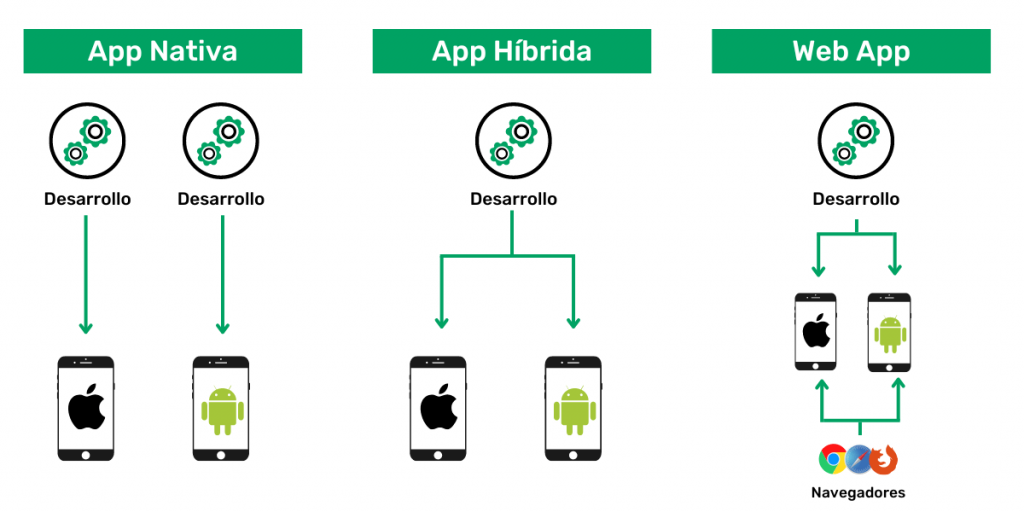
\includegraphics[width=.68\textwidth]{images/img08}}
		\caption{Tipo de aplicaciones moviles \cite{IM1}.}
		\label{fig:casosDeUso}
	\end{center}
\end{figure}

\subsection{Aplicaciones nativas}
Las aplicaciones nativas son apps desarrolladas para un sistema operativo móvil concreto (iOS o Android normalmente), en el lenguaje de programación específico de cada plataforma. Esto quiere decir que una app nativa creada para Android no puede ser utilizada en un dispositivo iOS y viceversa. \\

Es el tipo de aplicación móvil más conocida. Para que funcione, debemos descargarla desde los markets de apps, como App Store o Google Play e instalarla en nuestro teléfono \cite{CitaA02}.

\subsection*{Ventajas}
\begin{itemize}
	\item \textbf{Tienen el mejor rendimiento.} Las aplicaciones nativas son las más rápidas y tienen un rendimiento superior a otros tipos de apps, ya que han sido optimizadas específicamente para el hardware y el sistema operativo del dispositivo.
	\item \textbf{Acceso completo e integración con las funciones hardware del dispositivo.} Las apps nativas permiten aprovechar al máximo las funcionalidades móviles: cámara, micrófono, lector biométrico de huella, sensores y redes inalámbricas.
	\item \textbf{Pueden funcionar sin acceso a internet (funcionamiento offline)} si han sido diseñadas para ello.
\end{itemize}

\subsection*{Desventajas}
\begin{itemize}
	\item \textbf{Costes de desarrollo altos.} Si queremos tener nuestra app disponible para los dos sistemas, necesitaremos dos líneas de desarrollo diferentes, ya que el código utilizado para un sistema no es reutilizable para otro.
	\item \textbf{Complejidad de desarrollo.} Necesitamos equipos expertos en el lenguaje específico de cada sistema. Por ejemplo, en Kotlin para Android y en Swift para iOS.
	\item \textbf{Tiempo de desarrollo superior.} El desarrollo puede tomar entre 4 a 6 meses.
\end{itemize}

\subsection{Aplicaciones Web}

Las aplicaciones web realmente son webs especiales diseñadas para navegadores móviles. A diferencia de las apps nativas o híbridas, no necesitan ser descargadas, ya que se accede a ellas desde un navegador web.

Emplean las mismas tecnologías de desarrollo que una web, como HTML, CSS o JavaScript. Así, estaríamos hablando de una web con apariencia de app, por lo que presentaría sus mismas limitaciones. Sin embargo, con la llegada del HTML5, se han conseguido salvar algunas limitaciones, como el acceso a algunas funciones del móvil (geolocalización, cámaras) \cite{IM1}.

\subsection*{Ventajas}
\begin{itemize}
	\item \textbf{Carácter multiplataforma.} Con una sola línea de desarrollo.
	\item \textbf{Fácil desarrollo.} Se emplean tecnologías ampliamente conocidas.
	\item \textbf{Tiempo y coste de desarrollo bajo.}
\end{itemize}

\subsection*{Desventajas}
\begin{itemize}
	\item \textbf{Acceso limitado a las funciones del dispositivo.}
	\item \textbf{No se pueden subir a las tiendas de aplicaciones.}
	\item \textbf{Diferentes experiencias de usuario.} Estas dependen del navegador utilizado.
	\item \textbf{Necesidad de conexión a Internet.} Incluso si se cuenta con un modo pensado para ello, es necesario para acceder a las posibles actualizaciones o para entrar por primera vez.
\end{itemize}

\subsection{Aplicaciones Híbridas}

Las aplicaciones híbridas o multiplataforma combinan elementos de las aplicaciones nativas y las aplicaciones web. Estas aplicaciones se desarrollan utilizando tecnologías web como HTML, CSS y JavaScript, pero se empaquetan en un formato que puede ser instalado en un dispositivo móvil como cualquier otra aplicación nativa. Por tanto, podemos obtener una aplicación para varias plataformas con un único desarrollo \cite{IM1}.

\subsection*{Ventajas}
\begin{itemize}
	\item \textbf{Menor coste.} Gracias al uso de lenguajes de programación más conocidos, con una mayor disponibilidad de profesionales en el mercado.
	\item \textbf{Carácter multiplataforma.} Con una sola línea de desarrollo.
	\item \textbf{Acceso a algunas funcionalidades del móvil.}
	\item \textbf{Reducción de los tiempos de desarrollo.} Generalmente, el tiempo de desarrollo se reduce a 3 meses.
	\item \textbf{Disponibilidad en markets.} Se pueden subir a los markets de aplicaciones, como App Store y Google Play.
\end{itemize}

\subsection*{Desventajas}
\begin{itemize}
	\item \textbf{Rendimiento inferior.} Su rendimiento es inferior al de una app nativa, suelen tener un tamaño considerable y, además, ser más lentas.
	\item \textbf{Acceso limitado a las funciones del dispositivo.}
\end{itemize}

\subsection{Aplicaciones Progresivas Web Apps (PWA)}

Las aplicaciones progresivas son un reciente avance de las Web Apps. Al igual que las Web Apps, son webs diseñadas para móviles, pero esta vez, sí pueden ser descargadas en el móvil como una aplicación más, aunque no es necesario para que ofrezcan un comportamiento similar al de una app nativa a través del navegador. \\

Las PWA adoptan un comportamiento más propio de aplicaciones nativas que de web, como el funcionamiento sin Internet, un mayor rendimiento o su funcionamiento en segundo plano. Sin embargo, como desventaja, seguimos contando con la imposibilidad de subirlas a los markets de aplicaciones \cite{IM1}. \\

Para comprender mejor las diferencias entre los tipos de aplicaciones móviles, a continuación se presenta una tabla comparativa que destaca sus características clave:
\newpage

\begin{table}[h!]
	\centering
	\begin{tabular}{|p{4cm}|p{2cm}|p{2cm}|p{2cm}|}
		\hline
		\textbf{Tipos de app} & \textbf{Nativa} & \textbf{Híbrida} & \textbf{Web} \\ \hline
		\textbf{Interfaz} & Basada en web & Específica de la plataforma (iOS, Android) & Basada en web \\ \hline
		\textbf{Tiempo de desarrollo} & Alto & Medio & Bajo \\ \hline
		\textbf{Coste de desarrollo} & Alto & Medio & Bajo \\ \hline
		\textbf{Multiplataforma} & No & Sí & Sí \\ \hline
		\textbf{Rendimiento} & Alto & Medio & Bajo \\ \hline
		\textbf{Acceso a los sensores del dispositivo} & Completo & Alto o Completo & Limitado \\ \hline
		\textbf{Tiendas de aplicaciones} & Sí & Sí & No \\ \hline
	\end{tabular}
	\caption{Comparación tipos de aplicaciones móviles. Elaboración propia}
	\label{tab:tipos_apps}
\end{table}

Para el desarrollo de nuestro trabajo terminal, hemos decidido optar por una aplicación híbrida con el uso de Kotlin. Esta decisión se basa en varios factores relacionados con los recursos disponibles, las características de nuestro público objetivo y los plazos establecidos. \\

La aplicación móvil está dirigida para estudiantes, alumnos y personal de seguridad de la Escuela Superior de Cómputo, donde la mayoría utiliza dispositivos con sistema operativo Android. La elección de una aplicación híbrida nos permite optimizar  la experiencia en Android, que es la plataforma que predomina entre nuestros usuarios. \\

Aunque las aplicaciones híbridas suelen desarrollarse con tecnologías web (como React Native o Flutter), para nuestro proyecto hemos decidido incorporar Kotlin para desarrollar modelos donde se requiera un rendimiento nativo o un acceso más profundo a las funciones del sistema operativo Android.Además, las aplicaciones híbridas permiten un desarrollo más rápido en comparación con las aplicaciones completamente nativas, ya que gran parte del código puede compartirse entre plataformas, así mismo, es una buena opción económica que se adapta a nuestro presupuesto \cite{IM1}. 


%---------------------------------------------------------
% !TeX root = ../ejemplo.tex

\section{Sistema operativo}

%---------------------------------------------------------
% !TeX root = ../ejemplo.tex

\section{Lenguaje de programación}

%---------------------------------------------------------
% !TeX root = ../ejemplo.tex

\section{Framework}
\subsection{Jetpack compose}
Para la implementación de la aplicación móvil que forma parte de nuestro sistema de identificación y control de acceso, hemos decidido utilizar Jetpack Compose. La elección de la tecnología adecuada es importante para ofrecer una mejor experiencia de usuario y cumplir nuestros objetivos de diseño y funcional. 

\subsection*{¿Por que Jetpack compose?}
Jetpack compose es un framework (estructura o marco de trabajo que, bajo parámetros estandarizados, ejecutan tareas específicas en el desarrollo de un software) con la particularidad de ejecutar prácticas modernas en los desarrolladores de software a partir de la reutilización de componentes, así como también contando con la oportunidad de crear animaciones y temas oscuros. En este sentido, Jetpack Compose es el conjunto de herramientas ofrecidas por Android para el desarrollo de aplicaciones con un objetivo específico: simplificar y optimizar los códigos en la IU nativas \cite{CitaA01}. 


\subsection*{Ventajas}

\begin{itemize}
	\item \textbf{Menos código:} Simplifica el proceso de desarrollo haciendo menos código, todo se basa en funciones de modo que el código será simple y fácil de mantener.
	\item \textbf{Intuitiva:} Tan solo describe tu IU con un enfoque declarativo haciendo “qué hay que hacer” en vez de “cómo se debe hacer”.
	\item \textbf{Potente:} Tiene integrado Material Design con el cual puede crear apps atractivas al usuario con animaciones y mucho más.
	\item \textbf{Acelera el desarrollo:} Es compatible con proyectos existentes, puedes empezar a integrarlo por partes cuando quieras y donde quieras.
	\item \textbf{Kotlin:} Está escrito 100\% en Kotlin, lo cual nos permitirá usar sus herramientas potentes y API’s intuitivas.
\end{itemize}
%---------------------------------------------------------
% !TeX root = ../ejemplo.tex


\subsection{XML}
Para este proyecto utilizaremos XML debido a la múltiples ventajas que ofrece en el desarrollo de interfaces de usuario en aplicaciones web y Android\cite{CitaA03} .  

\subsection*{¿Por que XML?}

XML son siglas de \textit{Extensible Markup Language}, es un lenguaje de marcado que proporciona reglas para definir cualquier dato.

Por ejemplo, imaginemos un documento de texto con comentarios. Los comentarios pueden ofrecer sugerencias como las siguientes:
\begin{itemize}
	\item Ponga el título en negrita.
	\item Esta oración es un encabezado.
	\item Esta palabra es del autor.
\end{itemize}

Estos comentarios mejoran la usabilidad del documento sin repercutir en su contenido. Del mismo modo, XML utiliza símbolos de marcado para proporcionar más información sobre los datos.

\subsection*{Etiquetas XML}

Los s\'{\i}mbolos de marcado, denominados \textbf{etiquetas} en XML, se utilizan para definir los datos. Por ejemplo, para representar los datos de una librer\'{\i}a, se pueden crear etiquetas como:

\texttt{\textless libro\textgreater}, \texttt{\textless t\'{\i}tulo\textgreater} y \texttt{\textless autor\textgreater}

El documento XML de un solo libro tendr\'{\i}a el siguiente contenido:

\begin{lstlisting}
	<libro>
	<titulo>Introduccion a Amazon Web Services</titulo>
	<autor>Mark Wilkins</autor>
	</libro>
\end{lstlisting}


Las etiquetas ofrecen una sofisticada codificaci\'{o}n de datos para integrar los flujos de informaci\'{o}n en diferentes sistemas \cite{CitaA04}.

\subsection*{Ventajas de XML}

\begin{itemize}
	\item \textbf{Flexibilidad:} El formato XML es un lenguaje de marcas que se puede personalizar para diferentes prop\'{o}sitos.
	\item \textbf{Interoperabilidad:} El formato XML es compatible con una amplia gama de sistemas y aplicaciones, lo que significa que los datos se pueden intercambiar f\'{a}cilmente entre diferentes sistemas.
	\item \textbf{Legibilidad:} El formato XML es f\'{a}cil de leer y entender, lo que facilita la creaci\'{o}n y el mantenimiento de archivos XML.
	\item \textbf{Reutilizaci\'{o}n:} Los elementos y atributos de un archivo XML se pueden reutilizar en diferentes partes del archivo, lo que ahorra tiempo y reduce errores.
\end{itemize}


\chapter{Análisis}

%=========================================================
%=========================================================
\chapter{Modelo del Alcance}
\label{cap:reqUsr}

	En este capítulo se modela el alcance del sistema, se presentan  los requerimientos de usuario identificados y un diagrama de arquitectura de la solución propuesta junto con la especificación de plataforma correspondiente.

%---------------------------------------------------------

%---------------------------------------------------------


\section{Requerimientos de usuario}

En la siguiente tabla se enlistan los requerimientos de usuario identificados, estos corresponden a necesidades de los usuarios que harán uso del sistema. Se encuentran organizados por un Id único, el nombre del requerimiento, su descripción y su prioridad, que no es más que un análisis sobre su impacto en el desarrollo del sistema. 

\cdtInstrucciones{
	Identifique y describa los requerimientos funcionales del sistema señalando: id, nombre, descripción y prioridad.
}


\begin{requerimientosU}
	\FRitem{RU1}{Confirmar la asistencia a ETS}{Los alumnos quieren garantizar que su asistencia a la evaluación sea registrada.}{Alta}
	\FRitem{RU2}{Garantizar el acceso seguro y eficaz a las instalaciones.}{Los alumnos necesitan acceder a las instalaciones de forma rápida y segura, los días de aplicación a ETS.}{Alta}
	\FRitem{RU3}{Brindar alternativas para la identificación de alumnos.}{Los alumnos solicitan medios alternativos a los convencionales para autenticar su identidad.}{Media}
	\FRitem{RU4}{Confirmar la identidad de los alumnos presentes.}{Los docentes aplicadores quieren garantizar que los alumnos presentes estén inscritos al ETS}{Alta}
	\FRitem{RU5}{Reducir el tiempo del pase de lista.}{Los docentes aplicadores necesitan registrar la asistencia de los alumnos de manera rápida.}{Media}
	\FRitem{RU6}{Conocer los ETS inscritos.}{Los alumnos necesitan conocer los detalles de los ETS que van a presentar y el/la docente que lo impartirá.}{Media}
	\FRitem{RU7}{Conocer los ETS a impartir.}{Los docentes aplicadores necesitan conocer los detalles del ETS que supervisarán como el horario y lugar de aplicación.}{Media}
	\FRitem{RU8}{Conocer a los alumnos que presentaran ETS.}{Los docentes aplicadores necesitan conocer la información de los alumnos que están inscritos al ETS a aplicar.}{Media}
	\FRitem{RU9}{Conocer los horarios de aplicación de ETS.}{El personal de seguridad necesita conocer los horarios de aplicación de ETS para permitir o no la entrada de los estudiantes.}{Media}
	\FRitem{RU10}{Limitar el acceso a las instalaciones durante los ETS.}{El personal de seguridad necesita negar el acceso a la ESCOM a personas ajenas a la institución.}{Alta}
	\FRitem{RU11}{Registrar accesos a las instalaciones los días de aplicación de ETS}{El personal de seguridad necesita registrar los alumnos que acceden a las instalaciones para posterior consulta en caso de cualquier aclaración o imprevisto.}{Alta}
	\FRitem{RU12}{Comprobar los accesos a la institución en horarios oportunos.}{El personal de seguridad espera que los alumnos accedan en horarios congruentes con la aplicación de los ETS.}{Media}
	\FRitem{RU13}{Proteger la información personal.}{Los alumnos quieren mantener sus datos personales seguros.}{Alta}
	\FRitem{RU14}{Mantener separado las funciones y los datos de docentes y alumnos.}{Los docentes y alumnos esperan tener una ayuda personalizada para sus necesidades y no ver datos innecesarios.}{Media}
	\FRitem{RU15}{Mantener un recordatorio de eventos.}{Tanto los alumnos como docentes necesitan ser recordados sobre la información acerca de los ETS inscritos / asignados.}{Media}
	\FRitem{RU16}{Conocer las políticas de acceso a las instalaciones.}{Los alumnos quieren tener en claro cómo funciona el proceso de acceso a las instalaciones y qué documentos o pasos deben seguir para ingresar a las instalaciones los días de ETS.}{Media}
	\FRitem{RU17}{Minimizar los errores al verificar la identidad de los alumnos.}{Los docentes buscan minimizar la posibilidad de verificar de forma errónea la identidad de los alumnos.}{Alta}
	\FRitem{RU18}{Agilizar los procedimientos para la verificación de la identidad de los alumnos.}{Los docentes buscan minimizar los tiempos empleados en verificar la identidad de los alumnos presentes para la aplicación de los ETS.}{Alta}
	\FRitem{RU19}{Conocer fechas importantes del calendario escolar.}{Los alumnos, profesores y personal de seguridad necesitan conocer las fechas importantes del periodo escolar actual, incluyendo las relacionadas con los ETS.}{Baja}
	\FRitem{RU20}{Flexibilidad al aplicar ETS.}{Los profesores necesitan una alternativa que les permita delegar la responsabilidad de supervisar un ETS.}{Media}
	\FRitem{RU21}{Flexibilidad al aplicar ETS.}{Los profesores necesitan una alternativa que les permita delegar la responsabilidad de supervisar un ETS.}{Media}
	\FRitem{RU22}{Verificación de métodos de autenticación.}{Los alumnos requieren garantizar que los métodos de autenticación utilizados sean robustos y justos.}{Alta}
	\FRitem{RU23}{Control de ETS}{El personal de gestión escolar necesita gestionar la inscripción de los alumnos a los ETS.}{Media}
	\FRitem{RU24}{Control de trabajadores}{El personal de gestión escolar necesita gestionar los trabajadores adscritos al plantel educativo.}{Media}
	\FRitem{RU25}{Registro de alumnos.}{El personal de la DAE requiere dar de alta alumnos.}{Media}
	\FRitem{RU26}{Generación de credenciales de alumnos.}{El personal de la DAE requiere tomar fotografías de los alumnos para generar sus credenciales institucionales.}{Media}
	
	\caption{Requerimientos de usuario identificados.}
	{\footnotesize\em Para leer correctamente esta tabla vea la leyenda en la Tabla~\ref{tbl:leyendaRF} en la página~\pageref{tbl:leyendaRF}.}
	\label{tbl:reqFunc}	
	\end{requerimientosU}
	
   




%---------------------------------------------------------
\section{Especificación de plataforma}

A continuación se presenta la especificación de plataforma para aclarar el tipo de solución propuesta junto con un diagrama para establecer el patrón de arquitectura a utilizar.

\cdtInstrucciones{
	Coloque un diagrama y su descripción para aclarar el tipo de solución propuesta. \\
	
 En esta sección se debe aclarar:
	
\begin{description}
	\item[Tipo de sistema:] Aplicación híbrida, (aplicación móvil y sistema web para la gestión de estudiantes y exámenes)
	\item[Software requerido:] Python, SpringBoot, Java, Kotlin, bases de datos relacional PostgreSQL, base de datos vectorial (Pinecone).
	\item[Servicios:] De conexión, seguridad, firewall, respaldo de energía, redundancia, uso de raids, etc.
\end{description}
}

\begin{figure}[htbp!]
	\begin{center}
		\fbox{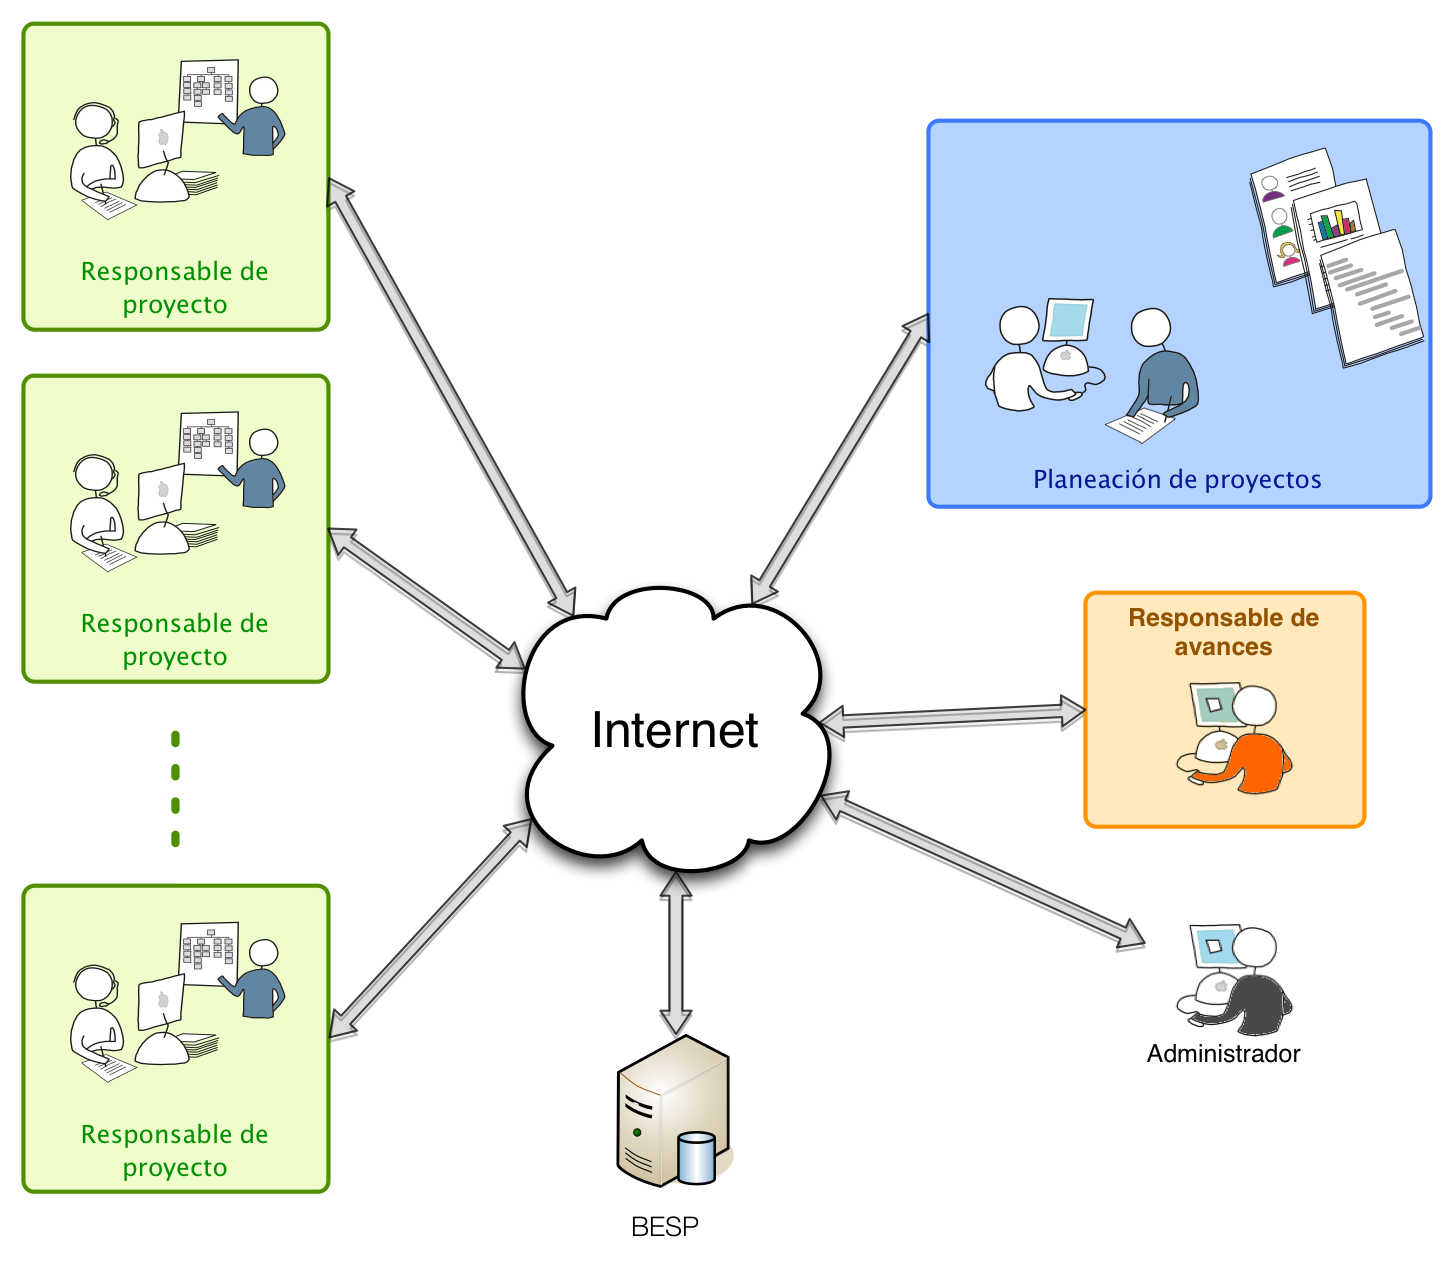
\includegraphics[width=.6\textwidth]{images/arquitectura}}
		\caption{Arquitectura del sistema.}
		\label{fig:arquitectura}
	\end{center}
\end{figure}

En la figura~\ref{fig:arquitectura} se describe la arquitectura general del sistema en la que se destaca el uso de un enfoque basado en micro-servicios, identificando los principales servicios que conforman la propuesta de solución y sus componentes principales.


%=========================================================
\section{Modelo del Negocio}	
\label{cap:reqSist}

	En está sección se modela la {\em Arquitectura del negocio} la cual está conformada por la Ontología del negocio ({\em Términos} y {\em Hechos del negocio}), Arquitectura de procesos y las {\em Reglas del negocio}. Primero se especifica brevemente el {\em Contexto} en el que los términos tienen significado.
		
	En las sección \ref{sec:terminosDeNegocio} se presentan los Términos del negocio a manera de Glosario y por último se presentan los Hechos del negocio a manera de relaciones entre términos del negocio.


%----------------------------------------------------------
\subsection{Contexto}

	\cdtInstrucciones{El contexto debe explicar bajo que ambiente los términos del negocio son aplicables y proporcionar información general para su comprensión inicial.\\}
	
	
%---------------------------------------------------------
\subsection{Términos del Negocio}
\label{sec:terminosDeNegocio}

\begin{description}
	% Ejemplo de un término literal.
	 \item[\hypertarget{tUnidadAcademica}{Unidad académica:}] Se refiere a la institución educativa en donde los usuarios se desenvuelven diariamente.
	
	\item[\hypertarget{tUnidadAprendizaje}{Unidad de aprendizaje:}] Son los elementos que componen un plan de estudios de alguna de las carreras ofertadas en la \hyperlink{tUnidadAcademica}{unidad académica}. Es necesario que los alumnos acrediten todas sus materias para continuar con su formación académica.
	
	\item[\hypertarget{tETS}{Exámen a Título de Suficiencia (ETS):}] Prueba final que permite a los alumnos acreditar una materia reprobada, y para la cual se requiere verificación de identidad.
	
	\item[\hypertarget{tAlumno}{Alumno:}] (es un tipo de Usuario) Se refiere a las personas inscritas dentro de algún plan de estudios ofertado en la \hyperlink{tUnidadAcademica}{unidad académica}.
	
	\item[\hypertarget{tDocenteAplicador}{Docente aplicador:}] (es un tipo de Usuario) Se refiere a las personas registradas como trabajadores que dan clases a los alumnos y supervisan los ETS asignados.
	
	\item[\hypertarget{tPersonalSeguridad}{Personal de seguridad:}] (es un tipo de Usuario) Se refiere a las personas registradas como trabajadores y que permiten o no el acceso a la \hyperlink{tUnidadAcademica}{unidad académica}.
	
	\item[\hypertarget{tCodigoQR}{Código QR:}] Código único generado por el sistema que permite resolver tareas de control de acceso a las instalaciones y a servicios de autenticación.
	
	\item[\hypertarget{tSistemaVerificacion}{Sistema de verificación de la identidad:}] Conjunto de procesos que permiten validar la identidad de los alumnos que buscan aplicar un ETS.
	
	\item[\hypertarget{tCredencialEscolar}{Credencial escolar:}] Documento con datos de identificación que pueden usarse junto a los registros de inscripción a ETS para permitir o no el acceso a la \hyperlink{tUnidadAcademica}{unidad académica}.
	
	\item[\hypertarget{tControlAcceso}{Control de acceso:}] Sistema implementado para verificar y autorizar el acceso a la \hyperlink{tUnidadAcademica}{unidad académica}.
	
	\item[\hypertarget{tRegistroAcceso}{Registro de acceso:}] Historial digital que documenta los accesos permitidos y denegados, incluyendo datos de cada intento de entrada para consulta posterior.
	
%	\brTermSensor{tVelocimetro}{Velocímetro:}{Velocidad de un Vehículo.}{Kilometros/hora.}{Constantemente siempre que el \cdtRef{tVehiculo}{vehículo} esté encendido.}
\end{description}
%---------------------------------------------------------


\subsection{Modelo del dominio del problema}
\label{sec:terminosDeNegocio}


\subsubsection{Modelo del dominio del problema}

El modelo del dominio del problema se muestra en la figura~\ref{fig:modeloDeDominio}, a continuación se describen cada una de las entidades y sus relaciones.

\newpage

\begin{figure}[htbp!]
	\begin{center}
		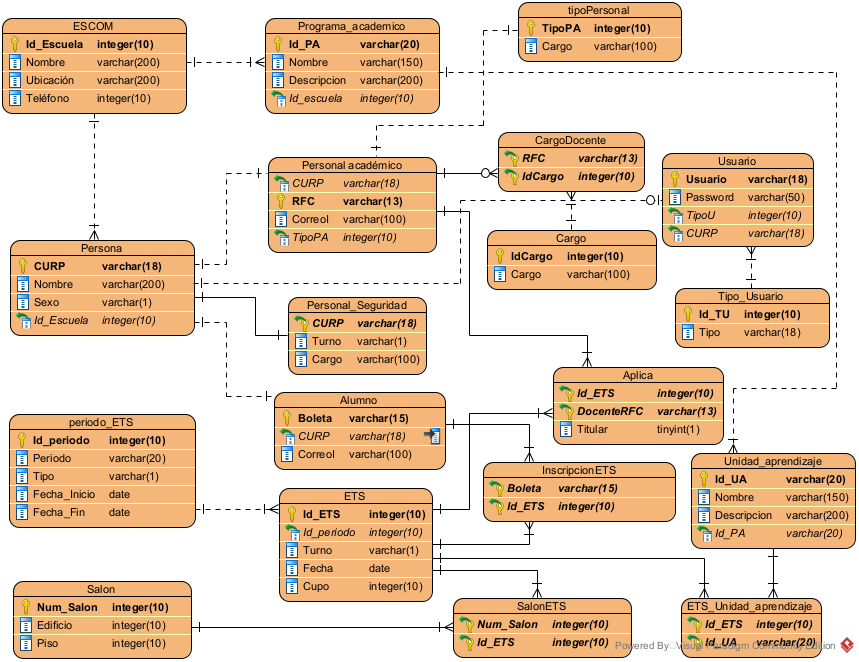
\includegraphics[angle=90,width=.85\textwidth]{images/DER}
		\caption{Modelo del dominio del problema}
		\label{fig:modeloDeDominio}
	\end{center}
\end{figure}

\newpage
%---------------------------------------------------------
\begin{cdtEntidad}{Unidad academica}{Unidad academica}
	\brAttr{Id\_escuela}{Id\_escuela}{Id}{Número de registro usado para identificar a la escuela.}{Sí}
	\brAttr{nombre}{Nombre}{Palabra}
	{Nombre de la escuela}{Sí}
%	\brAttr{ubicacion}{Ubicación}{Frase}
%	{Ubicación en la que se encuentra la escuela.}{Sí}
%	\brAttr{telefono}{Teléfono}{Teléfono}
%	{Teléfono para contactar a la escuela.}{Si}
%- - - - - - - - - - - - - - - - - - - - - - - - - - - - - 
	% \brRelComposition \brRelAgregation
%	\cdtEntityRelSection
%	\brRel{}{Programa\_académico}{ \hyperlink{Unidad academica}{Unidad académica} está compuesto por un \hyperlink{PA}{Programa académico}}	
%	\brRel{}{Persona}{Una \hyperlink{Persona}{Persona} pertenece a \hyperlink{Unidad academica}{Unidad academica}}	
\end{cdtEntidad}
%---------------------------------------------------------
\begin{cdtEntidad}{EscuelaPrograma}{Escuela\_Programa}
	\brAttr{Id\_Escuela}{Id\_Escuela}{Id}{Número de registro usado para identificar a la escuela.}{Sí}
	\brAttr{Id\_PA}{Id\_PA}{Id}
	{Identificación del programa académico que imparte la Unidad académica.}{Sí}
\end{cdtEntidad}
%---------------------------------------------------------
\begin{cdtEntidad}{PA}{Programa\_academico}
	\brAttr{Id\_PA}{Id\_PA}{Id}{Número de registro usado para identificar al programa académico.}{Sí}
	\brAttr{nombre}{Nombre}{Palabra}
	{Nombre del programa académico}{Sí}
	\brAttr{descripcion}{Descripción}{Frase}
	{Descripción que habla sobre el programa académico.}{Sí}
%- - - - - - - - - - - - - - - - - - - - - - - - - - - - -
%	\cdtEntityRelSection
%	\brRel{}{Unidad\_aprendizaje}{Un \hyperlink{PA}{Programa academico} está compuesto por una \hyperlink{UA}{Unidad de aprendizaje}}	
%	\brRel{}{Unidad academica}{Una \hyperlink{Unidad academica}{Unidad academica} está compuesta por un \hyperlink{PA}{Programa académico}}	
\end{cdtEntidad}
%---------------------------------------------------------
\begin{cdtEntidad}{Persona}{Persona}
	\brAttr{CURP}{CURP}{Id}{Código usado para identificar a las personas.}{Sí}
	\brAttr{nombre}{Nombre}{Frase corta}
	{Nombre(s) de la persona.}{Sí}
	\brAttr{ApellidoP}{Apellido\_P}{Frase corta}
	{Apellido paterno de la persona.}{Sí}
	\brAttr{ApellidoM}{Apellido\_M}{Frase corta}
	{Apellido materno de la persona.}{Sí}
	\brAttr{sexo}{Sexo}{Caracter}
	{Letra que servirá para identificar el sexo de un alumno ('M' para masculino, 'F' para femenino).}{Sí}
	\brAttr{Id\_escuela}{Id\_escuela}{Id}
	{Id de la escuela a la que pertenece la persona.}{Si}
	%- - - - - - - - - - - - - - - - - - - - - - - - - - - - -
%	\cdtEntityRelSection
%	\brRel{}{Unidad academica}{Una \hyperlink{Persona}{Persona} pertenece a una \hyperlink{Unidad academica}{Unidad academica}}	
%	\brRel{}{Docente}{Una \hyperlink{Persona}{Persona} es un \hyperlink{Docente}{Docente}}	
%	\brRel{}{Personal\_Seguridad}{Una \hyperlink{Persona}{Persona} es un \hyperlink{PS}{Personal de seguridad}}
%	\brRel{}{Alumno}{Una \hyperlink{Persona}{Persona} es un  \hyperlink{Alumno}{Alumno}}
%	\brRel{}{Usuario}{Una \hyperlink{Persona}{Persona} cuenta con un \hyperlink{Usuario}{Usuario}}
\end{cdtEntidad}
%---------------------------------------------------------
\begin{cdtEntidad}{PersonalAcademico}{Personal académico}
	\brAttr{CURP}{CURP}{Id}{Código usado para identificar a las personas.}{Sí}
	\brAttr{RFC}{RFC}{Id}
	{RFC que identifica al personal académico.}{Sí}
	\brAttr{CorreoI}{CorreoI}{Correo}
	{Correo institucional del personal académico.}{Sí}
	\brAttr{TipoPA}{TipoPA}{Id}{Número que identifica que tipo de personal académico es, ya sea, por ejemplo, un docente o personal de gestión escolar.}{Sí}
	%- - - - - - - - - - - - - - - - - - - - - - - - - - - - -
%	\cdtEntityRelSection
%	\brRel{}{CargoDocente}{Un \hyperlink{PersonalAcademico}{personal académico} puede ser un \hyperlink{CargoDocente}{Docente}}
%	\brRel{}{ETS}{Un \hyperlink{PersonalAcademico}{Docente} \hyperlink{Aplica}{Aplica} un \hyperlink{ETS}{ETS}}
%	\brRel{}{Persona}{Un \hyperlink{PersonalAcademico}{personal académico} es una \hyperlink{Persona}{Persona}}
%	\brRel{}{tipoPersonal}{Un \hyperlink{PersonalAcademico}{personal académico} tiene asignado un \hyperlink{Cargo}{Cargo}}
\end{cdtEntidad}
%---------------------------------------------------------
\begin{cdtEntidad}{tipoPA}{tipoPersonal}
	\brAttr{TipoPA}{TipoPA}{Id}
	{Número que identifica que tipo de personal académico es la persona.}{Sí}
	\brAttr{Cargo}{Cargo}{Frase corta}{Nombre del tipo de personal académico que tendrá la persona.}{Sí}
\end{cdtEntidad}
%---------------------------------------------------------
\begin{cdtEntidad}{CargoDocente}{CargoDocente}
	\brAttr{RFC}{RFC}{Id}
	{RFC que identifica al Docente.}{Sí}
	\brAttr{IdCargo}{IdCargo}{Id}{Código usado para identificar un cargo dentro de la escuela.}{Sí}
\end{cdtEntidad}
%---------------------------------------------------------
\begin{cdtEntidad}{Cargo}{Cargo}
	\brAttr{IdCargo}{IdCargo}{Id}{Código usado para identificar un cargo dentro de la escuela.}{Sí}
	\brAttr{Cargo}{Cargo}{Frase corta}
	{Nombre del cargo existente dentro de la institución escolar.}{Sí}
	%- - - - - - - - - - - - - - - - - - - - - - - - - - - - -
%	\cdtEntityRelSection
%	\brRel{}{CargoDocente}{Un \hyperlink{Cargo}{Cargo} es asignado a un \hyperlink{PersonalAcademico}{Docente}}
\end{cdtEntidad}
%---------------------------------------------------------
\begin{cdtEntidad}{PS}{Personal\_Seguridad}
	\brAttr{CURP}{CURP}{Id}{Código usado para identificar a las personas.}{Sí}
	\brAttr{Turno}{Turno}{Caracter}
	{Letra usada identificar el turno en el que se aplica el ETS ('M' para matutino, 'V' para vespertino).}{Sí}
	\brAttr{Cargo}{Cargo}{Frase corta}
	{Nombre del cargo del personal de seguridad.}{Sí}
	%- - - - - - - - - - - - - - - - - - - - - - - - - - - - -
	\cdtEntityRelSection
	\brRel{}{Persona}{Un \hyperlink{PS}{Personal de seguridad} es una \hyperlink{Persona}{Persona}}
\end{cdtEntidad}
%---------------------------------------------------------
\begin{cdtEntidad}{CargoPS}{CargoPS}
	\brAttr{Id\_Cargo}{Id\_Cargo}{Id}{Código usado para identificar el cargo que tiene el personal de seguridad.}{Sí}
	\brAttr{Nombre}{Nombre}{Frase corta}
	{Nombre del cargo del personal de seguridad.}{Sí}
	\brAttr{Cargo}{Cargo}{Frase corta}
	{Nombre del cargo del personal de seguridad.}{Sí}
\end{cdtEntidad}
%---------------------------------------------------------
\begin{cdtEntidad}{Alumno}{Alumno}
	\brAttr{Boleta}{Boleta}{Id}
	{Código usado para identificar al alumnado de la institución}{Sí}
	\brAttr{CURP}{CURP}{Id}{Código usado para identificar a las personas.}{Sí}
	\brAttr{CorreoI}{CorreoI}{Correo}
	{Correo institucional del alumno.}{Sí}
	\brAttr{Id\_PA}{Id\_PA}{Id}
	{Identificación del programa académico al que pertenece el alumno.}{Sí}
	%- - - - - - - - - - - - - - - - - - - - - - - - - - - - -
%	\cdtEntityRelSection
%	\brRel{}{Persona}{Un \hyperlink{Alumno}{Alumno} es una \hyperlink{Persona}{Persona}}
%	\brRel{}{ETS}{Un \hyperlink{Alumno}{Alumno} tiene una \hyperlink{InscripcionETS}{inscripción} a un \hyperlink{ETS}{ETS}}
\end{cdtEntidad}
%---------------------------------------------------------
\begin{cdtEntidad}{Usuario}{Usuario}
	\brAttr{Usuario}{Usuario}{Usuario}{Nombre de usuario asignado a una persona dentro del sistema.}{Sí}
	\brAttr{Password}{Password}{Contraseña}
	{Contraseña ligada al usuario de una persona registrada dentro del sistema.}{Sí}
	\brAttr{TipoU}{TipoU}{Id}
	{Número que identificará a los tipos de usuario registrados dentro del sistema.}{Sí}
	\brAttr{CURP}{CURP}{Id}
	{Código usado para identificar a las personas.}{Sí}
	%- - - - - - - - - - - - - - - - - - - - - - - - - - - - -
%	\cdtEntityRelSection
%	\brRel{}{Persona}{Un \hyperlink{Usuario}{Usuario} es asignado a una \hyperlink{Persona}{Persona}}
%	\brRel{}{Tipo\_Usuario}{Un \hyperlink{Usuario}{Usuario} tiene un \hyperlink{TU}{Tipo de usuario}}
\end{cdtEntidad}
%---------------------------------------------------------
\begin{cdtEntidad}{TU}{Tipo\_Usuario}
	\brAttr{Id\_TU}{Id\_TU}{Id}
	{RFC que identifica al personal académico.}{Sí}
	\brAttr{Tipo}{Tipo}{Frase corta}{Frase que definirá el tipo de usuario que tienen las personas.}{Sí}
\end{cdtEntidad}
%---------------------------------------------------------
\begin{cdtEntidad}{ETS}{ETS}
	\brAttr{Id\_ETS}{Id\_ETS}{Id}{Número usado para identificar los diferentes ETS registrados.}{Sí}
	\brAttr{Id\_periodo}{Id\_periodo}{Id}
	{Número usado para identificar el periodo en el que se realiza el ETS.}{Sí}
	\brAttr{Turno}{Turno}{Caracter}
	{Letra usada identificar el turno en el que se aplica el ETS ('M' para matutino, 'V' para vespertino).}{Sí}
	\brAttr{Fecha}{Fecha}{Fecha}
	{Fecha y hora en la que se realizará el ETS.}{Sí}
	\brAttr{Cupo}{Cupo}{Número}
	{Número de personas permitidas a realizar el ETS.}{Sí}
	\brAttr{Id\_UA}{Id\_UA}{Número}
	{Identificación de la Unidad de aprendizaje del ETS.}{Sí}
	\brAttr{Duracion}{Duracion}{Número}
	{Duración en horas del ETS.}{Sí}
	%- - - - - - - - - - - - - - - - - - - - - - - - - - - - -
%	\cdtEntityRelSection
%	\brRel{}{periodo\_ETS}{Un \hyperlink{ETS}{ETS} se realiza un en \hyperlink{PETS}{periodo}}
%	\brRel{}{Alumno}{En un \hyperlink{ETS}{ETS} está \hyperlink{InscripcionETS}{inscrito} un \hyperlink{Alumno}{Alumno}}
%	\brRel{}{Personal academico}{Un \hyperlink{ETS}{ETS} es \hyperlink{Aplica}{aplicado} por un \hyperlink{PersonalAcademico}{Docente}}
%	\brRel{}{Salon}{A un \hyperlink{ETS}{ETS} le \hyperlink{SalonETS}{corresponde} un \hyperlink{Salon}{Salón}}
%	\brRel{}{Unidad\_Aprendizaje}{Un \hyperlink{ETS}{ETS} \hyperlink{ETSUA}{es de} una \hyperlink{UA}{Unidad de Aprendizaje}.}
\end{cdtEntidad}
%---------------------------------------------------------
\begin{cdtEntidad}{PETS}{periodo\_ETS}
	\brAttr{Id\_periodo}{Id\_periodo}{Id}{Número usado para identificar el periodo en el que se realizarán los ETS registrados.}{Sí}
	\brAttr{Periodo}{Periodo}{Cadena de texto corta}
	{Periodo registrado en el que se realizarán los ETS.}{Sí}
	\brAttr{Tipo}{Tipo}{Caracter}
	{Letra usada identificar el tipo de los ETS que se aplicarán ('O' para ordinario, 'E' para especial).}{Sí}
	\brAttr{Fecha\_Inicio}{Fecha\_Inicio}{Fecha}
	{Fecha en la que iniciará el periodo de los ETS.}{Sí}
	\brAttr{Fecha\_Fin}{Fecha\_Fin}{Fecha}
	{Fecha en la que terminará el periodo de los ETS.}{Sí}
	%- - - - - - - - - - - - - - - - - - - - - - - - - - - - -
%	\cdtEntityRelSection
%	\brRel{}{ETS}{En un \hyperlink{PETS}{periodo de ETS} se realizan los \hyperlink{ETS}{ETS}.}
\end{cdtEntidad}
%---------------------------------------------------------
\begin{cdtEntidad}{Aplica}{Aplica}
	\brAttr{Id\_ETS}{Id\_ETS}{Id}{Número usado para identificar los diferentes ETS registrados.}{Sí}
	\brAttr{DocenteRFC}{DocenteRFC}{Id}
	{RFC que identifica al Docente.}{Sí}
	\brAttr{Titular}{Titular}{Booleano}
	{Booleano que identificará si el profesor que aplicará el ETS es el titular o es un ayudante.}{Sí}
\end{cdtEntidad}
%---------------------------------------------------------
\begin{cdtEntidad}{InscripcionETS}{InscripcionETS}
	\brAttr{Boleta}{Boleta}{Id}
	{Código usado para identificar al alumnado de la institución}{Sí}
	\brAttr{Id\_ETS}{Id\_ETS}{Id}{Número usado para identificar los diferentes ETS registrados.}{Sí}
\end{cdtEntidad}
%---------------------------------------------------------
\begin{cdtEntidad}{SalonETS}{SalonETS}
	\brAttr{Num\_Salon}{Num\_Salon}{Id}
	{Número usado para identificar al salón en el que se aplicará un ETS.}{Sí}
	\brAttr{Id\_ETS}{Id\_ETS}{Id}{Número usado para identificar los diferentes ETS registrados.}{Sí}
\end{cdtEntidad}
%---------------------------------------------------------
\begin{cdtEntidad}{Salon}{Salon}
	\brAttr{Num\_Salon}{Num\_Salon}{Id}
	{Número usado para identificar el salón en el que se aplicará un ETS.}{Sí}
	\brAttr{Edificio}{Edificio}{Número}
	{Número usado para identificar el edificio en el que se realizará el ETS.}{Sí}
	\brAttr{Piso}{Piso}{Número}
	{Número usado para identificar el piso del edificio en el que se realizará el ETS.}{Sí}
	\brAttr{TipoSalon}{TipoSalon}{Id}
	{Identificación del tipo de salón en el que se va a aplicar el ETS.}{Sí}
	%- - - - - - - - - - - - - - - - - - - - - - - - - - - - -
%	\cdtEntityRelSection
%	\brRel{}{ETS}{Un \hyperlink{Salon}{Salon} es \hyperlink{SalonETS}{ocupado} para llevar a cabo un \hyperlink{ETS}{ETS}.}
\end{cdtEntidad}
%---------------------------------------------------------
\begin{cdtEntidad}{TipoSalon}{TipoSalon}
	\brAttr{Num\_Salon}{Num\_Salon}{Id}
	{Número usado para identificar el salón en el que se aplicará un ETS.}{Sí}
	\brAttr{Tipo}{Tipo}{Frase corta}
	{Frase indicando el tipo de salón en el que se aplicará el ETS.}{Sí}
	%- - - - - - - - - - - - - - - - - - - - - - - - - - - - -
	%	\cdtEntityRelSection
	%	\brRel{}{ETS}{Un \hyperlink{Salon}{Salon} es \hyperlink{SalonETS}{ocupado} para llevar a cabo un \hyperlink{ETS}{ETS}.}
\end{cdtEntidad}
%---------------------------------------------------------
\begin{cdtEntidad}{UA}{Unidad\_aprendizaje}
	\brAttr{Id\_UA}{Id\_UA}{Id}
	{Identificación de la Unidad de Aprendizaje.}{Sí}
	\brAttr{Nombre}{Nombre}{Número}
	{Número usado para identificar el edificio en el que se realizará el ETS.}{Sí}
	\brAttr{Descripcion}{Descripcion}{Número}
	{Número usado para identificar el piso del edificio en el que se realizará el ETS.}{Sí}
	\brAttr{Id\_PA}{Id\_PA}{Id}
	{Número usado para identificar el piso del edificio en el que se realizará el ETS.}{Sí}
	%- - - - - - - - - - - - - - - - - - - - - - - - - - - - -
	\cdtEntityRelSection
	\brRel{}{ETS}{A una \hyperlink{UA}{Unidad de aprendizaje} le \hyperlink{ETSUA}{corresponde} una serie de \hyperlink{ETS}{ETS}.}
\end{cdtEntidad}
%---------------------------------------------------------
\subsection{Modelado de Reglas de negocio}

\begin{BussinesRule}{RN1}{Acceso al sistema.}
	\BRitem[Tipo:] Acceso. 
	\BRitem[Clase:] Condicional. 
	\BRitem[Nivel:] Estricto.
	\BRitem[Descripción:] El acceso a nuestro sistema será permitido solo para los Empleados y estudiantes de la ESCOM.
	\BRitem[Motivación:] Evitar el acceso no autorizado a otras personas que no sean de la ESCOM..

	\BRitem[Referenciado por:] \hyperlink{CU-01}{CU-01} y \hyperlink{CU41}{CU-41}.
\end{BussinesRule}

\begin{BussinesRule}{RN2}{ Acceso a las funcionalidades del docente.}
    \BRitem[Tipo:] Acceso. 
    \BRitem[Clase:] Condicional. 
    \BRitem[Nivel:] Estricto.
    \BRitem[Descripción:] Los docentes solo podrán acceder y revisar la información de los ETS que tengan asignados.
    \BRitem[Motivación:] Para evitar que los docentes se confundan, accedan a información que no les corresponde o modifiquen información que no les corresponde.

    \BRitem[Referenciado por:] \hyperlink{CU-01}{CU-01} y \hyperlink{CU-04}{CU-04}.
\end{BussinesRule}

\begin{BussinesRule}{RN3}{ Acceso a las funcionalidades del personal de seguridad.}
    \BRitem[Tipo:] Acceso. 
    \BRitem[Clase:] Condicional. 
    \BRitem[Nivel:] Estricto.
    \BRitem[Descripción:] El personal de seguridad solo podrán acceder y revisar la información relacionada con el acceso de los alumnos a la ESCOM de los días en los que se presenten ETS.
    \BRitem[Motivación:] Para evitar que el personal de seguridad se confunda, accedan a información que no les corresponde o modifiquen información que no les corresponde.

    \BRitem[Referenciado por:] \hyperlink{CU-01}{CU-01} y \hyperlink{CU-12}{CU-12}, \hyperlink{CU-13}{CU-13}, \hyperlink{CU-14}{CU-14} y \hyperlink{CU-15}{CU-15}.
\end{BussinesRule}

\begin{BussinesRule}{RN4}{ Acceso a las funcionalidades web}
	\BRitem[Tipo:] Habilitación.
	\BRitem[Clase:] Condicional.
	\BRitem[Nivel:] Estricta.
	\BRitem[Descripción:] El sistema permitirá únicamente a el personal de gestión escolar y al personal la DAE acceder al sistema web.
	\BRitem[Motivación:] Se necesita separar las funcionalidades de los empleados para que el sistema tenga cohesión y para que el sistema web no referencie al sistema movil.
	\BRitem[Referenciado por:] \hyperlink{CU-41}{CU-41}.
	\end{BussinesRule}

\begin{BussinesRule}{RN5} {Consultar periodos del docente}
	\BRitem[Tipo:] Habilitación.
	\BRitem[Clase:] Condicional.
	\BRitem[Nivel:] Estricta.
	\BRitem[Descripción:] El sistema permitirá únicamente a los docentes autenticados consultar los períodos de ETS que tiene asignados.
	\BRitem[Motivación:] Garantizar que solo usuarios autorizados consulten información sensible.			
	\BRitem[Referenciado por:] \hyperlink{CU-04}{CU-04}.
	\end{BussinesRule}

\begin{BussinesRule}{RN6} {Visualizar lista de alumnos inscritos}
	\BRitem[Tipo:] Acceso.
	\BRitem[Clase:] Condicional.
	\BRitem[Nivel:] Estricta.
	\BRitem[Descripción:] El sistema permitirá al docente consultar únicamente la lista de los alumnos inscritos a los ETS que le han sido asignados.
	\BRitem[Motivación:] Permitir que los docentes puedan visualizar la información de los estudiantes inscritos a los ETS que tenga asignados.
	\BRitem[Referenciado por:] \hyperlink{CU-09}{CU-09}.
	\end{BussinesRule}

\begin{BussinesRule}{RN7} {Acceso al asignar remplazo}
    \BRitem[Tipo:] Acceso.
    \BRitem[Clase:] Condicional.
    \BRitem[Nivel:] Estricta.
    \BRitem[Descripción:] El sistema permitirá solo al presidente de academia  y al jefe de departamento consultar la lista de solicitudes de remplazo y posteriormente asignar un remplazo.
    \BRitem[Motivación:] Hacer que solo el personal capacitado y responsable asigne los remplazos a los ETS.
    \BRitem[Referenciado por:] \hyperlink{CU-42}{CU-42}.
    \end{BussinesRule}

\begin{BussinesRule}{RN8} {Cantidad de pruebas de reconocimiento facial}
    \BRitem[Tipo:]Habilitación.
    \BRitem[Clase:]Cronometrada.
    \BRitem[Nivel:] Estricta.
    \BRitem[Descripción:] El alumno solo puede realizar un máximo de 3 pruebas de reconocimiento facial dentro de la aplicación.
    \BRitem[Motivación:] Evitar que el alumno le pida a alguien más que  pruebe constantemente el reconocimiento facial hasta que se parezca a el/ella.
    \BRitem[Referenciado por:] \hyperlink{CU-19}{CU-19}.
    \end{BussinesRule}

\begin{BussinesRule}{RN9} {Cantidad de intentos fallidos de inicio de sesión}
    \BRitem[Tipo:]Habilitación.
    \BRitem[Clase:] Cronometrada.
    \BRitem[Nivel:] Estricta.
    \BRitem[Descripción:] El sistema permitirá solo a todos los usuarios un máximo de 5 intentos de inicio de sesión fallidos antes de bloquear la cuenta del usuario.
    \BRitem[Motivación:] Asegurar la seguridad de los usuarios y evitar que personas no autorizadas entren al sistema.
    \BRitem[Referenciado por:] \hyperlink{CU-01}{CU-01}, y \hyperlink{CU-41}{CU-41}.
    \end{BussinesRule}

\begin{BussinesRule}{RN10} {Acceso a solo la información de los ETS }
    \BRitem[Tipo:]Habilitadora.
    \BRitem[Clase:]Condicional.
    \BRitem[Nivel:] Estricta.
    \BRitem[Descripción:] El sistema permitirá que los alumnos puedan ingresar solo a la información de sus ETS inscritos y solo consultar a la información (no podrán modificarla).
    \BRitem[Motivación:] Evitar que los alumnos cambien la información de los ETS y evitar que los alumnos sepan de otros alumnos que presentaran el mismo ETS (esto para no fomentar la formación de acuerdos entre los alumnos).
    \BRitem[Referenciado por:] \hyperlink{CU-19}{CU-19}.
    \end{BussinesRule}

% Alfredo

\begin{BussinesRule}{BR11}{Registro de usuarios válidos.} 
    \BRitem[Tipo:] Habilitadora
    \BRitem[Clase:] Integridad
    \BRitem[Nivel:] Estricta
    \BRitem[Descripción:] Todos los usuarios registrados dentro del sistema deberán de estar registrados dentro de la tabla “Persona”. 
    \BRitem[Motivación:] Asegurar que solo la comunidad de la institución pueda acceder a la escuela. 
    \BRitem[Referenciado por:] \hyperlink{Usuario}{Usuario} 
    \end{BussinesRule}

\begin{BussinesRule}{BR12}{Registro de personal académico.} 
    \BRitem[Tipo:] Habilitadora
    \BRitem[Clase:] Condición.
    \BRitem[Nivel:] Estricta
    \BRitem[Descripción:] Para registrar al personal académico se deberá de dar de alta un RFC, un correo institucional válido y especificar el cargo que tiene dentro de la institución. Este puede variar entre un docente o personal administrativo, como lo es el personal de gestión escolar. En caso de ser un docente se debe especificar su cargo dentro de la escuela, como lo es el jefe de academia, presidente de academia, director o subdirector. 
    \BRitem[Motivación:] Moderar los diferentes permisos de los usuarios dependiendo del cargo que tengan dentro de la escuela. 
    \BRitem[Referenciado por:] \hyperlink{PersonalAcademico}{Personal Académico} 
    \end{BussinesRule}

\begin{BussinesRule}{BR13}{Límite de alumnos en un ETS.} 
    \BRitem[Tipo:] Cronometrada. 
    \BRitem[Clase:] Condición.
    \BRitem[Nivel:] Estricta
    \BRitem[Descripción:] Un alumno se podrá inscribir a un ETS únicamente si la cantidad de alumnos aún no excede el cupo límite de un ETS.
    \BRitem[Motivación:] Evitar el sobrecupo de un salón el día del ETS.
    \BRitem[Referenciado por:] \hyperlink{ETS}{ETS} 
    \end{BussinesRule}
    
\begin{BussinesRule}{BR14}{Fecha de aplicación de los ETS.} 
    \BRitem[Tipo:] Cronometrada. 
    \BRitem[Clase:] Condición.
    \BRitem[Nivel:] Estricta
    \BRitem[Descripción:] Las fechas de los ETS deben de estar dentro del periodo especificado del mismo, en caso contrario no se podrá dar de alta. 
    \BRitem[Motivación:] Tener un control sobre las fechas en las que se aplican los ETS. 
    \BRitem[Referenciado por:] \hyperlink{ETS}{ETS} 
    \end{BussinesRule}

\begin{BussinesRule}{BR15}{Registro de un ETS} 
    \BRitem[Tipo:] Habilitadora. 
    \BRitem[Clase:] Condición.
    \BRitem[Nivel:] Estricta
    \BRitem[Descripción:] Los ETS deberán de especificar siempre el turno en el ques e van a aplicar, especificar el periodo en el que se aplican y el cupo que se tendrá para ese ETS.
    \BRitem[Motivación:] Tener un mejor control sobre la información de los ETS.
    \BRitem[Referenciado por:] \hyperlink{ETS}{ETS} 
    \end{BussinesRule}

\begin{BussinesRule}{BR16}{Asignación de salón para un ETS} 
    \BRitem[Tipo:] Habilitadora. 
    \BRitem[Clase:] Condición	.
    \BRitem[Nivel:] Estricta
    \BRitem[Descripción:] Un salón solo puede ser asignado a un ETS si no ha sido asignado para otro ETS.
    \BRitem[Motivación:] Evitar la sobreasignación de salones.
    \BRitem[Referenciado por:] \hyperlink{SalonETS}{Salón del ETS} 
    \end{BussinesRule}

\begin{BussinesRule}{BR17}{Permisos del usuario de los docentes.} 
    \BRitem[Tipo:] Ejecutiva.
    \BRitem[Clase:] Autorización.
    \BRitem[Nivel:] Estricta
    \BRitem[Descripción:] Si un docente tiene asignado más de un cargo dentro de la institución, el sistema le mostrará las interfaces correspondientes a cada uno de los cargos. El acceso a las interfaces dependerá de las funcionalidades permitidas por cada cargo.
    \BRitem[Motivación:] Asegurar que los docentes tengan acceso a todas las funciones dependiendo del cargo que tengan.
    \BRitem[Referenciado por:] \hyperlink{CargoDocente}{Cargo del docente} 
    \end{BussinesRule}

\begin{BussinesRule}{BR18}{Número de docentes aplicadores de un ETS.} 
    \BRitem[Tipo:] Habilitadora. 
    \BRitem[Clase:] Condición.
    \BRitem[Nivel:] Estricta
    \BRitem[Descripción:] Un mismo ETS puede ser aplicado por múltiples docentes en diferentes salones.
    \BRitem[Motivación:] Asegurar que todos los ETS tengan por lo menos un aplicador, ya sea en uno o más salones.
    \BRitem[Referenciado por:] \hyperlink{Aplica}{Tabla Aplica} 
    \end{BussinesRule}

\begin{BussinesRule}{BR19}{Inscripción de un ETS.} 
    \BRitem[Tipo:] Habilitadora. 
    \BRitem[Clase:] Autorización.
    \BRitem[Nivel:] Estricta
    \BRitem[Descripción:] Un alumno no puede estar inscrito en dos ETS que se lleven a cabo en el mismo horario.
    \BRitem[Motivación:] Evitar el solapamiento de dos o más ETS.
    \BRitem[Referenciado por:] \hyperlink{InscripcionETS}{Inscripción de un ETS} 
    \end{BussinesRule}

\begin{BussinesRule}{BR20}{Aplicador titular de un ETS.} 
    \BRitem[Tipo:] Integridad
    \BRitem[Clase:] Cronometrada.
    \BRitem[Nivel:] Estricta
    \BRitem[Descripción:] Los ETS deberán contar siempre con un docente titular que es el docente principal que va a aplicar el ETS. En caso de sustitución del docente o apoyo a este, también se especificará que estos son ayudantes y no titulares.
    \BRitem[Motivación:] Garantizar la asignación de roles dentro del sistema.
    \BRitem[Referenciado por:] \hyperlink{Aplica}{Tabla Aplica} 
    \end{BussinesRule}
    

%
\begin{BussinesRule}{RN21} {Acceso a información sobre el acceso a los ETS}
    \BRitem[Tipo:] Acceso.
    \BRitem[Clase:]Condicional.
    \BRitem[Nivel:] Estricta.
    \BRitem[Descripción:] El sistema permitirá que solo los alumnos puedan acceder a la información sobre los ETS en una pantalla.
    \BRitem[Motivación:] Permitir que los alumnos conozcan el proceso de acceso a los ETS y evitar confusiones y malentendidos.
    \BRitem[Referenciado por:] \hyperlink{CU-20}{CU-20}.
    \end{BussinesRule}

\begin{BussinesRule}{RN22} {Estructura de la CURP}
    \BRitem[Tipo:]Integridad.
    \BRitem[Clase:]Condicional.
    \BRitem[Nivel:] Estricta.
    \BRitem[Descripción:] La CURP debe de tener exactamente 18 caracteres y debe de poseer solo letras y números.
    \BRitem[Motivación:] Para mantener la estructura correcta de la CURP y evitar que se Introduzca datos inválidos.
    \BRitem[Referenciado por:] \hyperlink{CU-21}{CU-21}, \hyperlink{CU-22}{CU-22}, \hyperlink{CU-33}{CU-33} y \hyperlink{CU-37}{CU-37}.
    \end{BussinesRule}

\begin{BussinesRule}{RN23} {Estructura de la Boleta}
    \BRitem[Tipo:]Integridad.
    \BRitem[Clase:]Condicional.
    \BRitem[Nivel:] Estricta.
    \BRitem[Descripción:] La Boleta debe de tener exactamente 10 caracteres y debe de poseer solo números.
    \BRitem[Motivación:] Para mantener la estructura correcta de la Boleta y evitar que se Introduzca datos inválidos.
    \BRitem[Referenciado por:] \hyperlink{CU-21}{CU-21}, \hyperlink{CU-22}{CU-22}, \hyperlink{CU-33}{CU-33} y \hyperlink{CU-37}{CU-37}.
    \end{BussinesRule}

\begin{BussinesRule}{RN24} {Estructura del correo institucional del alumno}
    \BRitem[Tipo:]Integridad.
    \BRitem[Clase:]Condicional.
    \BRitem[Nivel:] Estricta.
    \BRitem[Descripción:] El correo institucional del alumno debe de seguir la estructura [texto][@][alumno.ipn.mx]
    \BRitem[Motivación:] Para mantener la estructura correcta del correo institucional y evitar que se Introduzca datos inválidos.
    \BRitem[Referenciado por:] \hyperlink{CU-21}{CU-21} y \hyperlink{CU-22}{CU-22}.
    \end{BussinesRule}

\begin{BussinesRule}{RN25} {Cantidad de alumnos por salud}
    \BRitem[Tipo:] Habilitación.
    \BRitem[Clase:] Cronometrada.
    \BRitem[Nivel:] Estricta.
    \BRitem[Descripción:] Los salones tienen un cupo máximo de 30 alumnos.
    \BRitem[Motivación:] Para evitar aglomeraciones de alumnos durante un ETS.
    \BRitem[Referenciado por:] \hyperlink{CU-21}{CU-21} y \hyperlink{CU-22}{CU-22}.
    \end{BussinesRule}

\begin{BussinesRule}{RN26} {Asignación de salones}
    \BRitem[Tipo:] Habilitación.
    \BRitem[Clase:] Cronometrada.
    \BRitem[Nivel:] Estricta.
    \BRitem[Descripción:] Los salones solo pueden ser asignados a un ETS durante un periodo de ETS concreto.
    \BRitem[Motivación:] Para evitar que los salones sean asignados a 2 o más ETS distintos a la vez.
    \BRitem[Referenciado por:] \hyperlink{CU-25}{CU-25}.
    \end{BussinesRule}

\begin{BussinesRule}{RN27} {Estructura del dato salón}
    \BRitem[Tipo:] Integridad.
    \BRitem[Clase:]Condicional.
    \BRitem[Nivel:] Estricta.
    \BRitem[Descripción:] El dato salón está conformado por 4 números de los cuales el primer indica el edificio, el segundo el piso y los otros dos el número del salón .
    \BRitem[Motivación:] Para mantener la estructura correcta del dato salón y evitar que se Introduzca datos inválidos.
    \BRitem[Referenciado por:] \hyperlink{CU-29}{CU-29}.
    \end{BussinesRule}

\begin{BussinesRule}{RN28} {Valores del turno }
    \BRitem[Tipo:]Integridad.
    \BRitem[Clase:]Condicional.
    \BRitem[Nivel:] Estricta.
    \BRitem[Descripción:] El turno solo puede ser matutino o vespertino.
    \BRitem[Motivación:] Para establecer que los ETS no se pueden hacer en periodos de tiempo irregulares.
    \BRitem[Referenciado por:] \hyperlink{CU-29}{CU-29} y \hyperlink{CU-33}{CU-33}.
    \end{BussinesRule}

\begin{BussinesRule}{RN29} {Fecha del ETS}
    \BRitem[Tipo:]Integridad.
    \BRitem[Clase:]Condicional.
    \BRitem[Nivel:] Estricta.
    \BRitem[Descripción:] La fecha del del ETS solo puede ser un día que este dentro del periodo del ETS asignado.
    \BRitem[Motivación:] Para establecer que los ETS no pueden estar fuera de la fecha del periodo de ETS asignado.
    \BRitem[Referenciado por:] \hyperlink{CU-29}{CU-29}.
    \end{BussinesRule}

\begin{BussinesRule}{RN30} {Selección de periodo de ETS para el ETS actual}
    \BRitem[Tipo:]Integridad.
    \BRitem[Clase:]Condicional.
    \BRitem[Nivel:] Estricta.
    \BRitem[Descripción:] Para dar de alta un ETS solo se puede poner el periodo de ETS actual o el más próximo si no hay actual.
    \BRitem[Motivación:] Para no asignar ETS en fechas imposibles.
    \BRitem[Referenciado por:] \hyperlink{CU-29}{CU-29}.
    \end{BussinesRule}


\begin{BussinesRule}{RN31} {Valores del tipo de periodo de ETS}
    \BRitem[Tipo:]Integridad.
    \BRitem[Clase:]Condicional.
    \BRitem[Nivel:] Estricta.
    \BRitem[Descripción:] El tipo del ETS solo puede ser ordinario o extraordinario.
    \BRitem[Motivación:] Para establecer correctamente los 2 tipos de ETS.
    \BRitem[Referenciado por:] \hyperlink{CU-25}{CU-25}.
    \end{BussinesRule}

\begin{BussinesRule}{RN32} {Asignación de fechas al periodo de ETS}
    \BRitem[Tipo:]Integridad.
    \BRitem[Clase:]Condicional.
    \BRitem[Nivel:] Estricta.
    \BRitem[Descripción:] Las fechas de inicio y de fin deben de ser validas.
    \BRitem[Motivación:] Para evitar asignar fechas de ETS imposibles.
    \BRitem[Referenciado por:] \hyperlink{CU-25}{CU-25}.
    \end{BussinesRule}

\begin{BussinesRule}{RN33} {Asignación de unidad de aprendizaje}
    \BRitem[Tipo:]Integridad.
    \BRitem[Clase:]Condicional.
    \BRitem[Nivel:] Estricta.
    \BRitem[Descripción:] La unidad de aprendizaje debe de estar registrada en el sistema.
    \BRitem[Motivación:] Para evitar asignar unidad de aprendizaje falsas.
    \BRitem[Referenciado por:] \hyperlink{CU-29}{CU-29}.
    \end{BussinesRule}

\begin{BussinesRule}{RN34} {Asignar sexo }
    \BRitem[Tipo:]Integridad.
    \BRitem[Clase:]Condicional.
    \BRitem[Nivel:] Estricta.
    \BRitem[Descripción:] El sexo de los usuarios se refiero al sexo biológico y no al género por lo que solo puede tomar el valor de masculino o femenino.
    \BRitem[Motivación:] Evitar confusiones y simplificar los daros guardados en la base de datos.
    \BRitem[Referenciado por:] \hyperlink{CU-21}{CU-21}, \hyperlink{CU-22}{CU-22}, \hyperlink{CU-33}{CU-33} y \hyperlink{CU-37}{CU-37}.
    \end{BussinesRule}

\begin{BussinesRule}{RN35} {Cantidad de fotos tomadas en la credencialización }
    \BRitem[Tipo:]Integridad.
    \BRitem[Clase:]Condicional.
    \BRitem[Nivel:] Estricta.
    \BRitem[Descripción:] Para la credencialización se tomaran 5 fotos.
    \BRitem[Motivación:] Para obtener datos para el entrenamiento de la red neuronal.
    \BRitem[Referenciado por:] \hyperlink{CU-22}{CU-22} y \hyperlink{CU-23}{CU-23}.
    \end{BussinesRule}

\begin{BussinesRule}{RN36} {Visualización del calendario escolar.}
    \BRitem[Tipo:] Acceso.
    \BRitem[Clase:] Condicional.
    \BRitem[Nivel:] Estricta.
    \BRitem[Descripción:] El sistema permitirá a los usuarios visualizar el calendario escolar completo, incluyendo las fechas programadas para los periodos de ETS.
    \BRitem[Motivación:] Permitir que los usuarios tengan acceso a la información actualizada del calendario escolar.
    \BRitem[Referenciado por:] \hyperlink{CU-02}{CU-02}.
    \end{BussinesRule}

\begin{BussinesRule}{RN37}{Actualizar del calendario escolar.}
    \BRitem[Tipo:] Habilitación.
    \BRitem[Clase:] Condicional.
    \BRitem[Nivel:] Estricta.
    \BRitem[Descripción:] El calendario escolar debe ser actualizado para reflejar cambios administrativos, y el sistema debe sincronizar esta información de manera automática.
    \BRitem[Motivación:] Asegurar que los usuarios tengan acceso a la información actualizada.
    \BRitem[Referenciado por:] \hyperlink{CU-02}{CU-02}.
    \end{BussinesRule}

\begin{BussinesRule}{RN38}{Visualizar de notificaciones.}
    \BRitem[Tipo:] Acceso.
    \BRitem[Clase:] Condicional.
    \BRitem[Nivel:] Estricta.
    \BRitem[Descripción:] El sistema permitirá a los usuarios revisar sus notificaciones.
    \BRitem[Motivación:] Permitir que los usuarios puedan visualizar las notificaciones de manera fácil.
    \BRitem[Referenciado por:] \hyperlink{CU-03}{CU-03}.
    \end{BussinesRule}

\begin{BussinesRule}{RN39}{Marcar de notificaciones como leídas.}
    \BRitem[Tipo:] Habilitación.
    \BRitem[Clase:] Condicional.
    \BRitem[Nivel:] Estricta.
    \BRitem[Descripción:] El sistema permitirá a los usuarios marcar una notificación como leída una vez que la hayan revisado.
    \BRitem[Motivación:] Facilitar la organización de las notificaciones.
    \BRitem[Referenciado por:] \hyperlink{CU-03}{CU-03}.
    \end{BussinesRule}

\begin{BussinesRule}{RN40}{Ordenar notificaciones.}
    \BRitem[Tipo:] Habilitación.
    \BRitem[Clase:] Condicional.
    \BRitem[Nivel:] Estricta.
    \BRitem[Descripción:] Las notificaciones deberán mostrarse ordenadas por fecha, de la más reciente a la más antigua.
    \BRitem[Motivación:] Mejorar la experiencia del usuario al priorizar las notificaciones más relevantes.
    \BRitem[Referenciado por:] \hyperlink{CU-03}{CU-03}.
    \end{BussinesRule}

\begin{BussinesRule}{RN41}{Consultar información de los ETS asignados.}
    \BRitem[Tipo:] Acceso.
    \BRitem[Clase:] Condicional.
    \BRitem[Nivel:] Estricta.
    \BRitem[Descripción:] El sistema debe permitir al docente visualizar la información de los ETS que le han sido asignados.
    \BRitem[Motivación:] Permitir que los docentes tengan acceso a la información de sus ETS asignados. 
    \BRitem[Referenciado por:] \hyperlink{CU-06}{CU-06}.
    \end{BussinesRule}

\begin{BussinesRule}{RN42}{Mostrar la información actualizada de los ETS.}
    \BRitem[Tipo:] Acceso.
    \BRitem[Clase:] Ejecutiva.
    \BRitem[Nivel:] Estricta.
    \BRitem[Descripción:] La información mostrada debe estar actualizada y reflejar cualquier cambio administrativo relacionado con los ETS asignados.
    \BRitem[Motivación:] Evitar inconsistencias en la información presentada al docente.
    \BRitem[Referenciado por:] \hyperlink{CU-06}{CU-06}.
    \end{BussinesRule}

\begin{BussinesRule}{RN43}{Filtrar los ETS por docente.}
    \BRitem[Tipo:] Acceso.
    \BRitem[Clase:] Condicional.
    \BRitem[Nivel:] Estricta.
    \BRitem[Descripción:] La información de los ETS asignados debe estar filtrada para que cada docente solo pueda visualizar los ETS que le correspondan.
    \BRitem[Motivación:] Proteger la privacidad de la información de otros docentes.
    \BRitem[Referenciado por:] \hyperlink{CU-06}{CU-06}.
    \end{BussinesRule}

\begin{BussinesRule}{RN44}{Visualizar la lista de alumnos inscritos.}
    \BRitem[Tipo:] Acceso.
    \BRitem[Clase:] Condicional.
    \BRitem[Nivel:] Estricta.
    \BRitem[Descripción:] El sistema permitirá al docente consultar la lista completa de los alumnos inscritos a un ETS asignado.
    \BRitem[Motivación:] Permitir al docente consultar la lista de alumnos inscritos que van a presentar un ETS que tenga asignado.
    \BRitem[Referenciado por:] \hyperlink{CU-08}{CU-08}.
    \end{BussinesRule}

\begin{BussinesRule}{RN45}{Mostrar información de alumnos.}
    \BRitem[Tipo:] Acceso.
    \BRitem[Clase:] Condicional.
    \BRitem[Nivel:] Estricta.
    \BRitem[Descripción:] La lista debe incluir información de los alumnos como Boleta, nombre completo y fotografía.
    \BRitem[Motivación:] Facilitar al docente la identificación de los alumnos durante el ETS.
    \BRitem[Referenciado por:] \hyperlink{CU-08}{CU-08}.
    \end{BussinesRule}

\begin{BussinesRule}{RN46}{Tomar asistencia de los alumnos inscritos a ETS.}
    \BRitem[Tipo:] Acceso.
    \BRitem[Clase:] Condicional.
    \BRitem[Nivel:] Estricta.
    \BRitem[Descripción:] El sistema permitirá al docente registrar la asistencia de los alumnos inscritos al ETS asignado.
    \BRitem[Motivación:] Garantizar que la asistencia solo sea tomada para los alumnos que están inscritos en el ETS.
    \BRitem[Referenciado por:] \hyperlink{CU-09}{CU-09}.
    \end{BussinesRule}

\begin{BussinesRule}{RN47}{Analizar la identidad del alumno.}
    \BRitem[Tipo:] Acceso.
    \BRitem[Clase:] Condicional.
    \BRitem[Nivel:] Estricta.
    \BRitem[Descripción:] El sistema deberá analizar el rostro de cada alumno y proporcionar un indicador comparando las características registradas y las detectadas por el reconocimiento facial.
    \BRitem[Motivación:] Facilitar el proceso pase de lista al docente. 
    \BRitem[Referenciado por:] \hyperlink{CU-09}{CU-09}.
    \end{BussinesRule}

\begin{BussinesRule}{RN48}{Mostrar la lista de asistencia de los alumnos.}
    \BRitem[Tipo:] Acceso.
    \BRitem[Clase:] Condicional.
    \BRitem[Nivel:] Estricta.
    \BRitem[Descripción:] El sistema permitirá al docente visualizar el estatus del pase de lista.
    \BRitem[Motivación:] Consultar los datos registrados previamente en el pase de lista.
    \BRitem[Referenciado por:] \hyperlink{CU-10}{CU-10}.
    \end{BussinesRule}

\begin{BussinesRule}{RN49}{Acceso autorizado para visualizar la información del alumno}
    \BRitem[Tipo:] Acceso.
    \BRitem[Clase:] Condicional.
    \BRitem[Nivel:] Estricta.
    \BRitem[Descripción:] El sistema permitirá a los docentes visualizar la información y foto de un alumno únicamente si tienen permisos autorizados.
    \BRitem[Motivación:] Garantizar que solo los docentes con autorización puedan consultar datos de los alumnos.
    \BRitem[Referenciado por:] \hyperlink{CU-11}{CU-11}.
    \end{BussinesRule}

\begin{BussinesRule}{RN50}{Privacidad de los datos de los alumnos.}
    \BRitem[Tipo:] .
    \BRitem[Clase:] Condicional.
    \BRitem[Nivel:] Estricta.
    \BRitem[Descripción:] La información y foto del alumno no podrán ser compartidas ni divulgadas sin el consentimiento del alumno.
    \BRitem[Motivación:] Proteger la privacidad y confidencialidad de los datos personales de los alumnos.
    \BRitem[Referenciado por:] \hyperlink{CU-11}{CU-11}.
    \end{BussinesRule}

\begin{BussinesRule}{RN51}{Validación de la credencial escolar.}
    \BRitem[Tipo:] Acceso, habilitacion o integridad
    \BRitem[Clase:] Condicional, Cronometrada o ejecutiva 
    \BRitem[Nivel:] Estricta.
    \BRitem[Descripción:] El sistema permitirá al personal de seguridad consultar la información de un alumno únicamente si se escanea correctamente el código QR de su credencial.
    \BRitem[Motivación:] Permitir que la información del alumno solo sea accesible por persona autorizado.
    \BRitem[Referenciado por:] \hyperlink{CU-12}{CU-12}.
    \end{BussinesRule}

\begin{BussinesRule}{RN52}{Consultar información por boleta}
    \BRitem[Tipo:] Habilitación.
    \BRitem[Clase:] Condicional.
    \BRitem[Nivel:] Estricta.
    \BRitem[Descripción:] El sistema requerirá el ingreso del número de boleta válido para buscar la información del alumno.
    \BRitem[Motivación:] Permitir que el personal de seguridad pueda consultar un alumno ingresando su boleta. 
    \BRitem[Referenciado por:] \hyperlink{CU-13}{CU-13}.
    \end{BussinesRule}

\begin{BussinesRule}{RN53}{Notificación de boleta no registrada.}
    \BRitem[Tipo:] Habilitación.
    \BRitem[Clase:] Condicional.
    \BRitem[Nivel:] Evitable.
    \BRitem[Descripción:] Si el número de boleta ingresado por el personal de seguridad no existe en la base de datos, el sistema notificará que el alumno no está registrado.
    \BRitem[Motivación:] Permitir que las búsquedas se limiten a registros existentes en la base de datos.
    \BRitem[Referenciado por:] \hyperlink{CU-13}{CU-13}.
    \end{BussinesRule}

\begin{BussinesRule}{RN54}{Consultar información por nombre}
    \BRitem[Tipo:] Habilitación.
    \BRitem[Clase:] Condicional.
    \BRitem[Nivel:] Estricta.
    \BRitem[Descripción:] El sistema requerirá el ingreso del nombre para buscar la información del alumno.
    \BRitem[Motivación:] Permitir que el personal de seguridad pueda consultar un alumno ingresando su nombre. 
    \BRitem[Referenciado por:] \hyperlink{CU-14}{CU-14}.
    \end{BussinesRule}

\begin{BussinesRule}{RN55}{Notificación de nombre no registrada.}
    \BRitem[Tipo:] Habilitación.
    \BRitem[Clase:] Condicional.
    \BRitem[Nivel:] Evitable.
    \BRitem[Descripción:] Si el nombre ingresado por el personal de seguridad no existe en la base de datos, el sistema notificará que el alumno no está registrado.
    \BRitem[Motivación:] Permitir que las búsquedas se limiten a registros existentes en la base de datos.
    \BRitem[Referenciado por:] \hyperlink{CU-14}{CU-14}.
    \end{BussinesRule}





	









%=========================================================
%=========================================================
\chapter{Modelo dinámico}	
\label{cap:modDinamico}

El presente capítulo describe el modelo dinámico de nuestro sistema propuesto. En este se explican y representan las interacciones entre los actores y las funcionalidades del sistema estructurando la información necesaria para comprender su funcionamiento y diseño para asegurar una implementación coherente y funcional.

En primer lugar, se describe la notación empleada para los diagramas de casos de uso, seguida de una pequeña explicación de porque decidimos establecer ciertos casos como necesarios y otros como no necesarios. Posteriormente, se introduce el diagrama de estructura de usuarios, que organiza a los actores según sus roles, después se describirán los actores que participaran en el sistema y se establecen sus responsabilidades y procesos. A partir de esto, se presentan los diagramas de casos de uso para los sistemas móvil y web, destacando las funcionalidades específicas de cada sistema. Finalmente, se proporciona una descripción exhaustiva de los casos de uso seleccionados como necesarios.

\section{Notación}

%\newpage

\begin{figure}[htbp!]
	\begin{center}
		\fbox{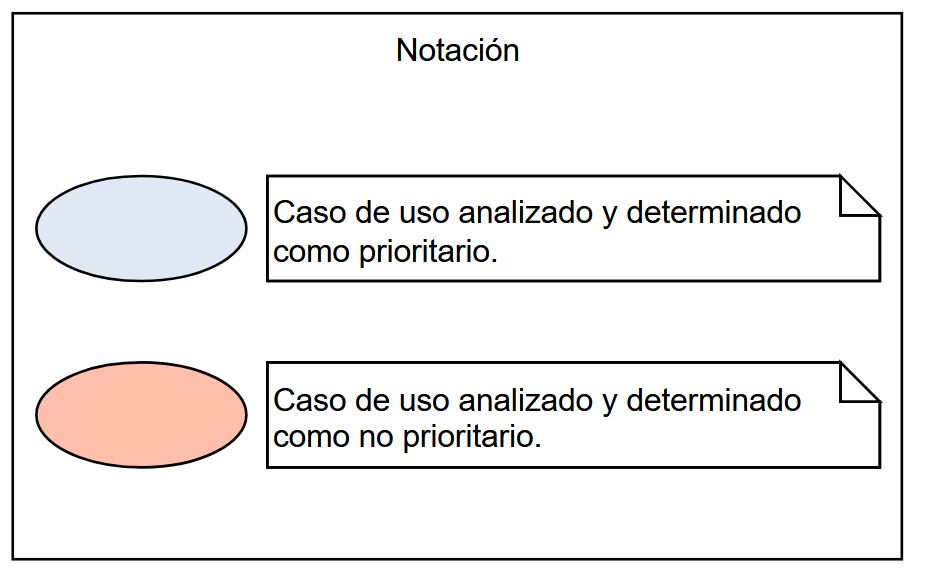
\includegraphics[width=.35\textwidth]{images/Notacion}}
		\caption{Análisis de viabilidad de los casos de uso.}
		\label{fig:Notacion}
	\end{center}
\end{figure}

Ahora comenzaremos con la explicación de la notación usada para el diagrama de casos de uso. En la figura \ref{fig:Notacion} se puede ver la notación usada para el diagrama de casos de uso, en este se puede observar que se usaron 2 colores para clasificarlos; los casos de uso de color azul fueron analizados y determinados como prioritarios y los casos de uso de color rojo fueron analizados y determinados como no prioritarios.

Decidimos determinar como casos de uso prioritarios a todos los casos del sistema móvil porque son los casos que son propios de nuestro sistema y son la parte principal de nuestro trabajo terminal y la más representativa ya que posee el mayor enfoque de inteligencia artificial, por otro lado, decidimos tomar los casos de uso del personal de la DAE como necesarios porque con ellos se justificaría la obtención de la credencial mediante el uso del proceso de la credencialización, también decidimos usar la parte de consultas y altas de los CRUD de: periodo de ETS, ETS, alumnos, docentes y personal de seguridad. Esto para representar los procesos que se realizan en el SAES y la DAE para mejorar el entendimiento, sin embargo, usar el resto del CRUD y los demás procesos de la DAE y el SAES quedan fuera del alcance del proyecto ya que se separan de la idea principal del trabajo terminal, además de que consumirán bastante tiempo y no están enfocados a la inteligencia artificial.

\section{Estructura de usuarios }

\begin{figure}[htbp!]
	\begin{center}
		\fbox{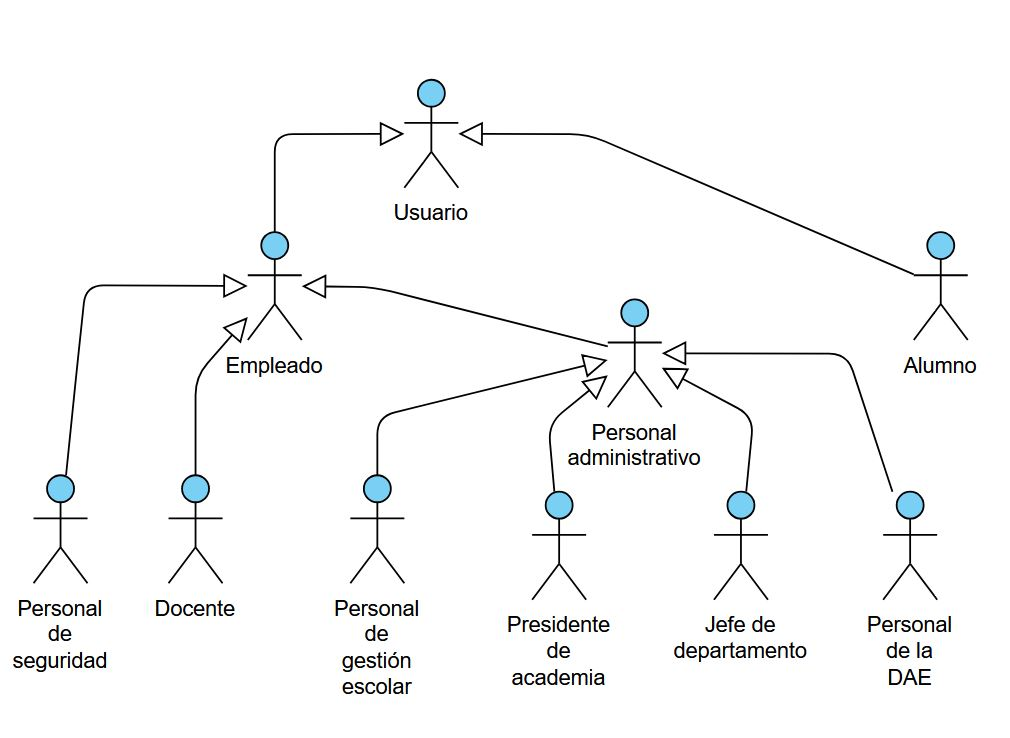
\includegraphics[width=.8\textwidth]{images/EstructuraU}}
		\caption{Estructura de los usuarios.}
		\label{fig:EstructuraU}
	\end{center}
\end{figure} 

En la figura \ref{fig:EstructuraU} se muestra la estructura de los usuarios y los tipos de usuario que están presentes en el sistema, en este se puede observar como todos los usuarios se derivan de un usuario general llamado usuario, posteriormente se divide en tipos; empleado y alumno. Después el empleado se subdivide dejando al personal de seguridad y al docente como empleados generales y creando un sub-usuario llamado personal administrativo el cual contiene al personal de gestión escolar, al presidente de academia, jefe de academia y al personal de la DAE. 

A continuación, se describirán las responsabilidades y los procesos de cada uno de los usuarios específicos (es decir los: los alumnos, personal de seguridad, docente, personal de gestión escolar, presidente de academia, jefe de departamento y personal de la DAE).

%\newpage



%\newpage

%\newpage



%---------------------------------------------------------
\section{Descripción de actores}

%---------------------------------------------------------
\begin{Usuario}{\hypertarget{tAlumno}{\subsection{Alumno}}}{
		Se refiere a las personas inscritas dentro de algún plan de estudios ofertado en la unidad académica.
	}
	\item[Responsabilidades:] \cdtEmpty
	\begin{itemize}
		\item Asistir puntualmente a las clases, prácticas y evaluaciones.
		\item Respetar a docentes, compañeros y personal administrativo.
		\item Cumplir con los requisitos y actividades de las asignaturas inscritas, incluyendo tareas, proyectos y exámenes.
		\item Realizar oportunamente los trámites escolares como inscripciones, reinscripciones, solicitudes de documentos oficiales, etc.
		\item Portar credencial institucional en todo momento.
	\end{itemize}
	

\end{Usuario}

\begin{Usuario}{\hypertarget{tPersonalSeguridad}{\subsection{Personal de seguridad}}}{
		Se refiere a las personas registradas como empleados y que permiten o no el acceso a la unidad académica.
	}
	\item[Responsabilidades:] \cdtEmpty
	\begin{itemize}
		\item Supervisar el acceso y la salida de alumnos, personal docente y visitantes, asegurándose de que cumplan con los protocolos establecidos.
		\item Verificar la identificación de las personas que ingresan a las instalaciones.
		\item Responder de manera oportuna a incidentes o emergencias dentro de las instalaciones.
		\item Brindar apoyo al personal, docentes o alumnos en caso de accidentes o situaciones de riesgo.
	\end{itemize}
	

\end{Usuario}

\begin{Usuario}{\hypertarget{tDocenteAplicador}{\subsection{Docente}}}{
		Se refiere a las personas registradas como empleados que dan clases a los alumnos y supervisan los ETS asignados.
	}
	\item[Responsabilidades:] \cdtEmpty
	\begin{itemize}
		\item Impartir las clases de manera clara, puntual y completa, cumpliendo con los objetivos de aprendizaje.
		\item Diseñar y aplicar instrumentos de evaluación justos, objetivos y alineados con los contenidos del curso.
		\item Orientar a los alumnos en el desarrollo de competencias y habilidades.
		\item Resolver dudas o problemáticas académicas dentro y fuera del aula, cuando sea necesario.
		\item Registrar la asistencia de los alumnos y reportar incidencias graves.
		\item Cumplir con la entrega de calificaciones y reportes en tiempo y forma.

	\end{itemize}
	

\end{Usuario}

\begin{Usuario}{\hypertarget{tPersonalGestion}{\subsection{Personal de gestión escolar}}}{
		Se refiere a las personas registradas como empleados y personal administrativo que realiza los procesos administrativos dentro de la ESCOM.
	}
	\item[Responsabilidades:] \cdtEmpty
	\begin{itemize}

		\item Gestionar el proceso de inscripción y reinscripción de los alumnos, verificando que cumplan con los requisitos establecidos.
		\item Mantener y actualizar el historial académico de los alumnos en los sistemas institucionales.
		\item Revisar y validar actas de nacimiento, certificados y otros documentos oficiales requeridos para el registro de los alumnos.
		\item Atender solicitudes y problemáticas relacionadas con registros, certificados, bajas temporales y procesos extraordinarios.
		\item Brindar orientación a alumnos y docentes sobre trámites escolares, fechas importantes y normatividad académica.
	\end{itemize}


\end{Usuario}

\begin{Usuario}{\hypertarget{tPersonalDAE}{\subsection{Personal de la DAE}}}{
		Se refiere a las personas registradas como empleados y personal administrativo que realiza los procesos administrativos dentro de la DAE.
	}
	\item[Responsabilidades:] \cdtEmpty
	\begin{itemize}

		\item Fomentar y coordinar actividades extracurriculares que complementen la formación académica, como talleres, conferencias, eventos culturales y deportivos.
		\item Supervisar programas de apoyo académico, como tutorías, orientación educativa y psicológica.
		\item Difundir información sobre programas de movilidad académica, intercambios, convenios nacionales e internacionales y programas de servicio social.
		\item Gestionar y emitir las credenciales oficiales del IPN para los alumnos.
		\item Verificar que los documentos requeridos para la emisión de la credencial estén completos y sean válidos.
		\item Coordinar el proceso de inscripción de los alumnos.
		\item Actualizar y mantener los registros académicos y administrativos de los alumnos. 
	\end{itemize}


\end{Usuario}

\begin{Usuario}{\hypertarget{tPresidente}{\subsection{Presidente de academia}}}{
	Se refiere a las personas registradas como empleados y personal administrativo que lidera la academia de una unidad académica o área de conocimiento dentro de la ESCOM.
	}
	\item[Responsabilidades:] \cdtEmpty
	\begin{itemize}

		\item Convocar y presidir las reuniones de academia, donde se toman decisiones sobre planes y programas de estudio.
		\item Coordinar la creación o actualización de planes y programas de estudio conforme a las necesidades del mercado laboral y las directrices institucionales.
		\item Verificar que los contenidos impartidos por los docentes sean consistentes con los objetivos de los programas.
		\item Detectar necesidades de capacitación entre los docentes y promover cursos o talleres. 
	\end{itemize}

\end{Usuario}

\begin{Usuario}{\hypertarget{tJefe}{\subsection{Jefe de departamento}}}{
	Se refiere a las personas registradas como empleados y personal administrativo que supervisa las actividades de una o más unidades académicas dentro de ESCOM.
}
\item[Responsabilidades:] \cdtEmpty
\begin{itemize}

	\item Administrar los recursos humanos y materiales asignados al departamento.
	\item Supervisar la implementación de los programas de estudio y el cumplimiento de los objetivos educativos.
	\item Promover y coordinar proyectos de investigación, desarrollo tecnológico o vinculación relacionados con el departamento.
	\item Atender quejas, sugerencias o problemas que surjan en el departamento, ya sea entre docentes o alumnos.
\end{itemize}

\end{Usuario}

\section{Diagramas de casos de uso}

A continuación se muestran los diagramas de casos de uso:

\begin{figure}[htbp!]
	\begin{center}
		\fbox{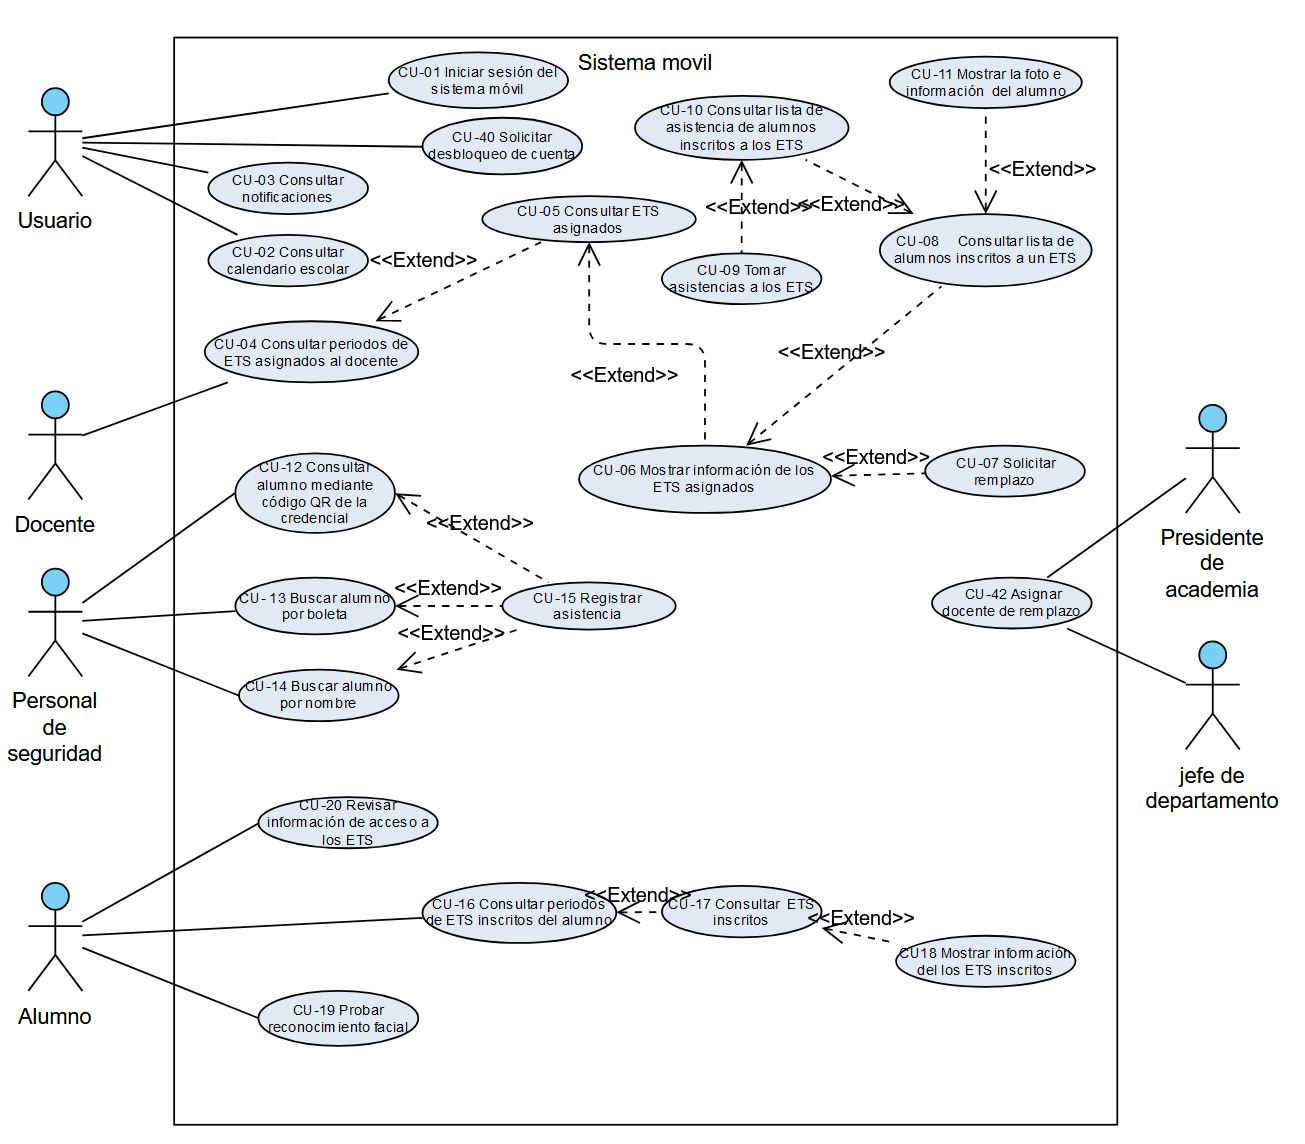
\includegraphics[width=.6\textwidth]{images/casosDeUso1}}
		\caption{Diagrama de casos de uso del sistema movil.}
		\label{fig:casosDeUso1}
	\end{center}
\end{figure}
En la figura \ref{fig:casosDeUso1} se muestra el diagrama de casos de uso del sistema móvil el cual es el sistema principal del trabajo terminal. En este diagrama se detalla la estructura del sistema, los casos de uso del docente, del alumno, del personal de seguridad, del presidente de academia y el jefe de departamento.
%\newpage
\begin{figure}[htbp!]
	\begin{center}
		\fbox{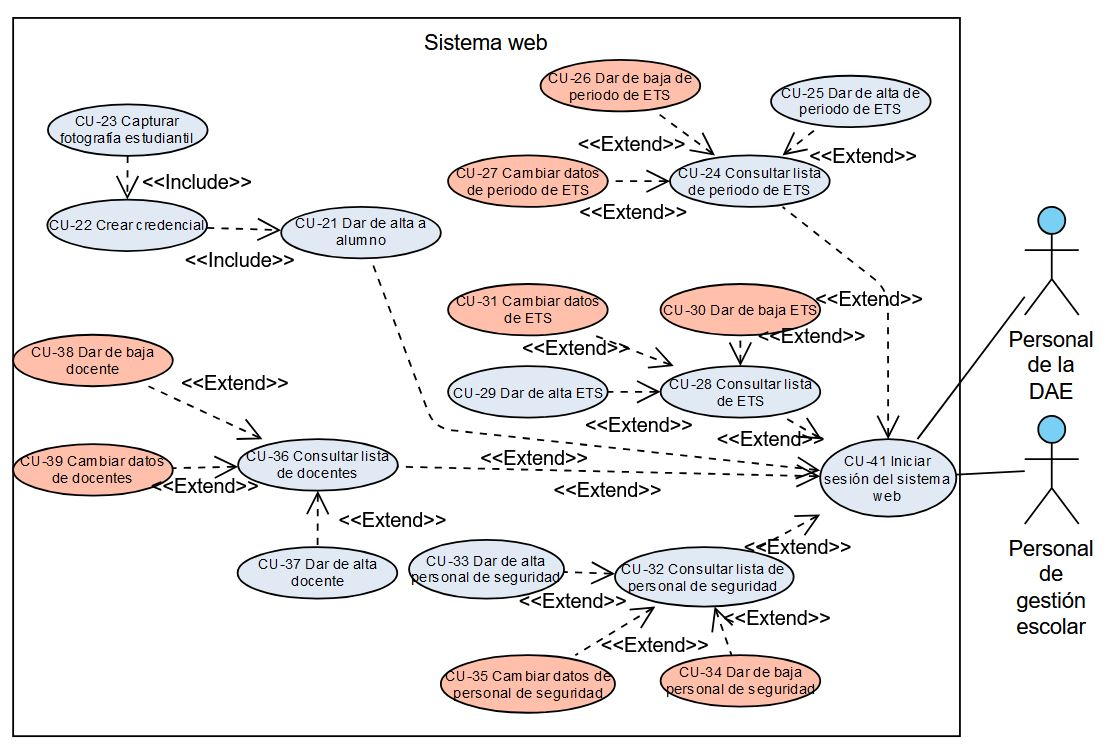
\includegraphics[width=.6\textwidth]{images/casosDeUso2}}
		\caption{Diagrama de casos de uso del sistema web.}
		\label{fig:casosDeUso2}
	\end{center}
\end{figure}

En la figura \ref{fig:casosDeUso2} se muestra el diagrama de casos de uso del sistema web el cual es el sistema secundario (la simulación de una parte del SAES y de la DAE) del trabajo terminal. En este diagrama se detalla la estructura del sistema, los casos de uso personal de la DAE y el personal de gestión escolar.

A continuación se detallan los casos de uso.

\section{Especificación de casos de uso }

%---------------------------------------------------------
% CASOS DE USO

% !TeX root = ../ejemplo.tex

%--------------------------------------
\begin{UseCase}{CU01}{Iniciar sesión de personal escolar móvil}{
		Permitir que solo el personal escolar pueda acceder al sistema, además de separar completamente las funciones del alumno y el personal escolar.
	}
	\UCitem{Versión}{\color{Gray}1}
	\UCitem{Autor}{\color{Gray}Huertas Ramírez Daniel Martín}
	\UCitem{Supervisa}{\color{Gray}Ulises Vélez Saldaña.}
	\UCitem{Actor}{\hyperlink{Empleado}{Empleado} (\hyperlink{Docente}{Docente} y \hyperlink{Personal de seguridad}{Personal de seguridad})}
	\UCitem{Propósito}{Que el empelado pueda acceder al sistema móvil y sus funciones específicas. }
	\UCitem{Entradas}{\hyperlink{Empleado.RFC}{RFC}, \hyperlink{Empleado.Contraseña}{Contraseña}}
	\UCitem{Origen}{Teclado}
	\UCitem{Salidas}{Saludo del sistema, mención de su nombre.}
	\UCitem{Destino}{Pantalla \IUref{IUE01}{Pantalla Menú de docente} si es un docente o a la \IUref{IUE02}{Pantalla Menú del personal de seguridad} si es un personal de seguridad.}
	\UCitem{Precondiciones}{El empleado debe estar registrado en el sistema de la ESCOM.}
	\UCitem{Postcondiciones}{El empleado accede al sistema y podrá realizar las acciones pertinentes a su cargo.}
	\UCitem{Errores}{
		E1: Cuando falte algún dato requerido entonces el sistema muestra el mensaje {\bf MSG1-}{``Los campos no están correctamente llenados.''}
		
		E2: Cuando la cuenta esta bloqueada el sistema no deja entrar al empleado muestra el mensaje {\bf MSG2-}``Su cuenta esta bloqueada.''
		
		E3: Cuando la contraseña no corresponde al RFC ingresado el sistema no permite el acceso al empleado y se muestra el mensaje {\bf MSG3-} ``El RFC o la contraseña no corresponden con ningún empleado.''
		
		E4: Cuando se pierde la conexión durante el proceso, los procesos se cancelan y se muestra el mensaje {\bf MSG4-}  ``El proceso no se pudo realizar por un falló de red.''
		
		E5: Cuando se intenta iniciar varias veces sesión sin éxito la cuenta es bloqueada por seguridad y se muestra el mensaje {\bf MSG5-}  ``Su cuenta ha sido bloqueada por la gran cantidad de intentos de inicio sesión fallidos''.
	}
	\UCitem{Tipo}{Caso de uso primario}
	\UCitem{Observaciones}{}
\end{UseCase}
%--------------------------------------

\begin{UCtrayectoria}
	\UCpaso[\UCactor] Introduce su RFC y contraseña en el sistema vía la \IUref{IU01}{Pantalla de Iniciar sesión de personal escolar móvil}\label{CU01.introduceDatos}.
	\UCpaso[\UCactor] Confirma la operación presionando el botón \IUbutton{Entrar}.
	\UCpaso Verifica que todos los datos requeridos hayan sido capturados.
	\UCpaso Verifica que el empleado este registrado en el sistema.
	\UCpaso Verifica que la cuenta del empleado no este bloqueada.
	\UCpaso Verifica que la contraseña corresponda al RFC.
	\UCpaso Verifica que tipo acceso tiene este empleado.
	\UCpaso La sesión es iniciada con éxito.
	\UCpaso El Empleado es redirigido a la pantalla \IUref{IUE01}{Pantalla Menú de docente} si es un docente o a la pantalla \IUref{IUE02}{Menú de personal de seguridad} si es un personal de seguridad.
	
\end{UCtrayectoria}







\newpage

% !TeX root = ../ejemplo.tex

%--------------------------------------
\begin{UseCase}{CU-02}{Consultar calendario escolar}{
    Permitir que los usuarios vean el calendario escolar y puedan solicitar al sistema que les mencioné cuantos días faltan para que inicie el próximo periodo de ETS.
}
    \UCitem{Versión}{\color{Gray}1}
    \UCitem{Autor}{\color{Gray}Huertas Ramírez Daniel Martín}
    \UCitem{Supervisa}{\color{Gray}De la Cruz de la Cruz Alejandra.}
    \UCitem{Actor}{\hyperlink{Usuario}{Usuario}}
    \UCitem{Propósito}{Que el usuario consulte cuantos días faltan para el próximo periodo de ETS.}
    \UCitem{Entradas}{Ninguna}
    \UCitem{Origen}{Pantalla táctil}
    \UCitem{Salidas}{Menciona cuantos días faltan para el periodo de ETS o si menciona que ya es periodo de ETS.}
    \UCitem{Destino}{Ninguno}
    \UCitem{Precondiciones}{El usuario debe de haber iniciado sesión.}
    \UCitem{Postcondiciones}{El usuario recibe información sobre la fecha del periodo de ETS actual.}
    \UCitem{Errores}{
        E1: Cuando es periodo de ETS el sistema muestra el mensaje {\bf MSG-6}{``Actualmente es periodo de ETS.''}

        E2: Cuando no se ha establecido un periodo de ETS actual, el sistema muestra el mensaje {\bf MSG-7}{``Actualmente el periodo de ETS no ha sido establecido.''}
    
    }
    \UCitem{Tipo}{Caso de uso primario}
    \UCitem{Observaciones}{Ninguna}
\end{UseCase}
%-------------------------------------- 

\begin{UCtrayectoria}
    \UCpaso[\UCactor] El usuario accede a la pantalla \IUref{IU02}{Pantalla Consultar calendario escolar}\label{CU02.introduceDatos} para la app móvil y \IUref{IU02-2}{Pantalla Consultar calendario escolar} para el sistema web mediante el botón con forma de calendario en cualquier pantalla excepto el inicio de sesión.
    \UCpaso[\UCactor] El usuario decide consultar cuantos días faltan para que el periodo de ETS inicie oprimiendo el botón\IUbutton{Calcular cuantos días faltan para el periodo de ETS}.
    \UCpaso El sistema calcula cuantos días faltan tomando el día actual y el día de inicio del periodo de ETS.
    \UCpaso El sistema regresa cuantos días faltan para que el periodo de ETS inicie.
    \UCpaso [\UCactor] El usuario verifica cuantos días faltan para que inicie el periodo de ETS.
\end{UCtrayectoria}








\newpage

% !TeX root = ../ejemplo.tex

%--------------------------------------
\begin{UseCase}{CU-03}{Consultar notificaciones}{
    Permitir a los usuarios revisar sus notificaciones con más detenimiento y establecerlas como leídas.
}
    \UCitem{Versión}{\color{Gray}1}
    \UCitem{Autor}{\color{Gray}Huertas Ramírez Daniel Martín}
    \UCitem{Supervisa}{\color{Gray}De la Cruz de la Cruz Alejandra.}
    \UCitem{Actor}{\hyperlink{Usuario}{Usuario}}
    \UCitem{Propósito}{Que el usuario revise sus notificaciones con detenimiento y las establezca como leídas.}
    \UCitem{Entradas}{Ninguna}
    \UCitem{Origen}{Pantalla táctil}
    \UCitem{Salidas}{Menciona que la notificación seleccionada ha sido establecida como leída.}
    \UCitem{Destino}{Ninguno}
    \UCitem{Precondiciones}{El usuario debe de haber iniciado sesión.}
    \UCitem{Postcondiciones}{El usuario revisó sus notificaciones.}
    \UCitem{Errores}{
        E1: Cuando el usuario no tiene notificaciones el sistema muestra el mensaje {\bf MSG-8}{``Actualmente no hay notificaciones.''}    
    }
    \UCitem{Tipo}{Caso de uso primario}
    \UCitem{Observaciones}{}

\end{UseCase}
%-------------------------------------- 

\begin{UCtrayectoria}
    \UCpaso[\UCactor] El usuario accede a la pantalla \IUref{IU03}{Pantalla Consultar notificaciones}\label{CU03.introduceDatos} para la app móvil  mediante el botón con forma de campana en cualquier pantalla excepto los inicios de sesión.
    \UCpaso[\UCactor] El usuario decide consultar sus notificaciones más actuales \Trayref{A}.
    \UCpaso[\UCactor] El usuario marco como leídas las notificaciones que acaba de leer mediante el botón con forma de palomita especifico de cada notificación.
    \UCpaso El sistema marca como leídas las notificaciones.

\end{UCtrayectoria}

\begin{UCtrayectoriaA}{A}{El usuario quiere consultar las notificaciones de una fecha específica}
	\UCpaso[\UCactor] El usuario usa el buscador de la parte superior para buscar notificaciones según su fecha.
	\UCpaso[\UCactor] El usuario marco como leídas las notificaciones que acaba de leer mediante el botón con forma de palomita especifico de cada notificación.
	\UCpaso El sistema marca como leídas las notificaciones.

\end{UCtrayectoriaA}



\newpage

% \IUref{IUAdmPS}{Administrar Planta de Selección}
% \IUref{IUModPS}{Modificar Planta de Selección}
% \IUref{IUEliPS}{Eliminar Planta de Selección}

%-------------------------------------- COMIENZA descripción del caso de uso.

%\begin{UseCase}[archivo de imágen]{UCX}{Nombre del Caso de uso}{
%--------------------------------------
\begin{UseCase}{CU-04}{Consultar periodos de ETS asignados al docente}{
		Este caso de uso permite al docente consultar los periodos de ETS que tiene asignados. 
	}
	\UCitem{Versión}{\color{Gray}1.0}
	\UCitem{Autor}{\color{Gray}De la cruz De la cruz Alejandra}
	\UCitem{Supervisa}{\color{Gray}Ulises Velez Saldaña}
	\UCitem{Actor}{\hyperlink{Docente}{Docente}}
	\UCitem{Propósito}{Permitir al docente consultar los periodos de ETS que le han sido asignados.}
	\UCitem{Entradas}{Ninguna}
	\UCitem{Origen}{Pantalla táctil}
	\UCitem{Salidas}{Lista de periodos de ETS asignados.}
	\UCitem{Destino}{\IUref{IU04}{Pantalla Periodo de ETS}}
	\UCitem{Precondiciones}{El docente debe estar autenticado en el sistema.}
	\UCitem{Postcondiciones}{El docente ha consultado los periodos de ETS asignados.}
	\UCitem{Errores}{
			E1:El sistema no puede recuperar la información de los periodos.
			
			E2: No hay periodos de ETS asignados al docente. }
	\UCitem{Tipo}{Se extiende del CU}
	\UCitem{Observaciones}{Ninguna}
\end{UseCase}
%--------------------------------------
\begin{UCtrayectoria}
	\UCpaso[\UCactor] Accede a la \IUref{IUE01}{Pantalla Menú del docente} después de haber iniciado sesión.
	\UCpaso[\UCactor] Presiona el botón \IUbutton{Consultar periodos de ETS}.
	\UCpaso Verifica que el docente cuente con periodos de ETS. \Trayref{A}.
	\UCpaso Busca en la base de datos los periodos de ETS asignados al docente.
	\UCpaso Despliega la lista de periodos de ETS asignados al docente en la \IUref{IU04}{Pantalla Periodo de ETS}.
\end{UCtrayectoria}
%--------------------------------------        
\begin{UCtrayectoriaA}{A}{No hay periodos asignados al docente}
	\UCpaso Verifica y no encuentra registros de periodos de ETS asignados al docente.
	\UCpaso Muestra un mensaje: {\bf MSG10-}{``No hay periodos de ETS asignados.''}
	\UCpaso[\UCactor] Presiona el botón \IUbutton{Regresar} para volver a la pantalla anterior.
	\UCpaso Fin de la trayectoria alternativa.
\end{UCtrayectoriaA}
%--------------------------------------        
\begin{UCtrayectoriaA}{B}{Error en la conexión con la base de datos}
	\UCpaso Muestra un mensaje de error: {\bf MSG11-}{``Error al consultar la base de datos. Intente nuevamente más tarde.''}
	\UCpaso[\UCactor] Presiona el botón \IUbutton{Aceptar} para cerrar el mensaje.
	\UCpaso[\UCactor] Puede intentar la consulta nuevamente o presionar el botón \IUbutton{Regresar} para volver a la pantalla anterior.
	\UCpaso Fin de la trayectoria alternativa.
\end{UCtrayectoriaA}
%-------------------------------------- TERMINA descripción del caso de uso.

\newpage

% \IUref{IUAdmPS}{Administrar Planta de Selección}
% \IUref{IUModPS}{Modificar Planta de Selección}
% \IUref{IUEliPS}{Eliminar Planta de Selección}

%-------------------------------------- COMIENZA descripción del caso de uso.

%\begin{UseCase}[archivo de imágen]{UCX}{Nombre del Caso de uso}{
%--------------------------------------
\begin{UseCase}{CU-05}{Consultar ETS asignados}{
		Este caso de uso permite al docente consultar los ETS que tiene asignados.
	}
	\UCitem{Versión}{\color{Gray}1.0}
	\UCitem{Autor}{\color{Gray}De la cruz De la cruz Alejandra}
	\UCitem{Supervisa}{\color{Gray}Ulises Velez Saldaña}
	\UCitem{Actor}{\hyperlink{Docente}{Docente}}
	\UCitem{Propósito}{Permitir al docente consultar los ETS que le han sido asignados.}
	\UCitem{Entradas}{Selecciona un periodo}
	\UCitem{Origen}{Pantalla táctil}
	\UCitem{Salidas}{Lista de ETS asignados.}
	\UCitem{Destino}{\IUref{IU05}{Pantalla de Consultar ETS}}
	\UCitem{Precondiciones}{El docente debe estar autenticado en el sistema.}
	\UCitem{Postcondiciones}{El docente ha consultado los ETS asignados.}
	\UCitem{Errores}{
			E1: El sistema no puede recuperar la información de los ETS asignados.
			
			E2: No hay ETS asignados al docente.}
	\UCitem{Tipo}{Se extiende del CU01 Iniciar Sesión del docente}
	\UCitem{Observaciones}{Ninguna}
\end{UseCase}
%--------------------------------------
\begin{UCtrayectoria}
	\UCpaso[\UCactor] Selecciona el período académico que desea consultar desde la \IUref{IU04}{Pantalla Periodo de ETS}.
	\UCpaso Verifica que el docente tenga ETS asignados en el periodo seleccionado \Trayref{A}.
	\UCpaso Despliega la lista de ETS asignados al docente en la \IUref{IU05}{Pantalla de Consultar ETS}.
\end{UCtrayectoria}

%--------------------------------------        
\begin{UCtrayectoriaA}{A}{No hay ETS asignados en el periodo seleccionado}
	\UCpaso Muestra un mensaje: {\bf MSG-12-}{``No hay ETS asignados actualmente.''}
	\UCpaso[\UCactor] Presiona el botón \IUbutton{Regresar} para volver a la pantalla anterior.
	\UCpaso Fin de la trayectoria alternativa.
\end{UCtrayectoriaA}
%--------------------------------------        
\begin{UCtrayectoriaA}{B}{Error en la conexión con la base de datos}
	\UCpaso Muestra un mensaje de error: {\bf MSG11-}{``Error al consultar la base de datos. Intente nuevamente más tarde.''}
	\UCpaso[\UCactor] Presiona el botón \IUbutton{Aceptar} para cerrar el mensaje.
	\UCpaso[\UCactor] Puede intentar la consulta nuevamente o presionar el botón \IUbutton{Regresar} para volver a la pantalla anterior.
	\UCpaso Fin de la trayectoria alternativa.
\end{UCtrayectoriaA}

%-------------------------------------- TERMINA descripción del caso de uso.
\newpage

% \IUref{IUAdmPS}{Administrar Planta de Selección}
% \IUref{IUModPS}{Modificar Planta de Selección}
% \IUref{IUEliPS}{Eliminar Planta de Selección}

%-------------------------------------- COMIENZA descripción del caso de uso.

%\begin{UseCase}[archivo de imágen]{UCX}{Nombre del Caso de uso}{
%--------------------------------------
% !TeX root = ../ejemplo.tex
\begin{UseCase}{CU-06}{Mostrar información de los ETS asignados}{
	Este caso de uso permite al docente visualizar la información detallada de los ETS que tiene asignados.
}
\UCitem{Versión}{\color{Gray}1.0}
\UCitem{Autor}{\color{Gray}De la cruz De la cruz Alejandra}
\UCitem{Supervisa}{\color{Gray}Huertas Ramírez Daniel Martín}
\UCitem{Actor}{\hyperlink{PersonalAcademico}{Docente}}
\UCitem{Propósito}{Permite al docente visualizar la información detallada de cada ETS que tiene asignado.}
\UCitem{Entradas}{Ninguna}
\UCitem{Origen}{Pantalla táctil}
\UCitem{Salidas}{Detalle de ETS asignado.}
\UCitem{Destino}{\IUref{IU06}{Pantalla Información de ETS}}
\UCitem{Precondiciones}{El docente debe estar autenticado y tener ETS asignados en el sistema.}
\UCitem{Postcondiciones}{El docente ha visualizado la información detallada de sus ETS asignados.}
\UCitem{Errores}{
		E1: El sistema no puede recuperar la información detallada de los ETS y muestra el mensaje {\bf MSG-12}{``Información no disponible para el ETS seleccionado''}.
		E2: Error en la conexión con la base de datos y muestra el mensaje y muestra el mensaje {\bf MSG-9}{``Error al consultar la base de datos. Intente nuevamente más tarde.''}.
}
\UCitem{Tipo}{Se entiende del CU-05 Mostrar información de los ETS asignados}
\UCitem{Observaciones}{Ninguna}
\end{UseCase}
%--------------------------------------
\begin{UCtrayectoria}
\UCpaso[\UCactor] El docente selecciona el ETS que desea visualizar desde la \IUref{IU05}{Pantalla  Consultar ETS}.
\UCpaso[\UCsist] El sistema verifica si existen detalles disponibles para el ETS seleccionado. \Trayref{A}
\UCpaso El sistema despliega la información detallada de cada ETS asignado en la \IUref{IU06}{Pantalla Información de ETS}
\end{UCtrayectoria}
%--------------------------------------        
\begin{UCtrayectoriaA}{A}{No hay detalles disponibles para el ETS seleccionado}
\UCpaso El sistema muestra un mensaje: {\bf MSG-12}{``Información no disponible para el ETS seleccinado''}
\UCpaso[\UCactor] El docente presiona el botón \IUbutton{Regresar} para volver a la lista de ETS.
\UCpaso Fin de la trayectoria alternativa.
\end{UCtrayectoriaA}

%--------------------------------------        
\begin{UCtrayectoriaA}{B}{Error en la conexión con la base de datos}
\UCpaso El sistema muestra un mensaje de error: {\bf MSG-9}{``Error al consultar la base de datos. Intente nuevamente más tarde.''}
\UCpaso[\UCactor] El docente presiona el botón \IUbutton{Aceptar} para cerrar el mensaje.
\UCpaso[\UCactor] El docente puede intentar la consulta nuevamente o presionar el botón \IUbutton{Regresar} para volver a la pantalla anterior.
\UCpaso Fin de la trayectoria alternativa.
\end{UCtrayectoriaA}

%-------------------------------------- TERMINA descripción del caso de uso.


\newpage

% \IUref{IUAdmPS}{Administrar Planta de Selección}
% \IUref{IUModPS}{Modificar Planta de Selección}
% \IUref{IUEliPS}{Eliminar Planta de Selección}

%-------------------------------------- COMIENZA descripción del caso de uso.

%\begin{UseCase}[archivo de imágen]{UCX}{Nombre del Caso de uso}{
%--------------------------------------
\begin{UseCase}{CU-07}{Asignar docente ayudante}{
		Este caso de uso permite a un docente solicitar la asignación de un docente ayudante para aplicar el ETS en su lugar en caso de no poder asistir.
	}
	\UCitem{Versión}{\color{Gray}1.0}
	\UCitem{Autor}{\color{Gray}De la cruz De la cruz Alejandra}
	\UCitem{Supervisa}{\color{Gray}Ulises Velez Saldaña}
	\UCitem{Actor}{\hyperlink{Docente}{Docente}}
	\UCitem{Propósito}{Permitir al docente asignado para un ETS solicitar ayuda de otro docente para realizar la aplicación en su lugar.}
	\UCitem{Entradas}{
		\begin{itemize}
			\item Identificador del ETS.
			\item Identificador del docente ayudante solicitado.
		\end{itemize}
	}
	\UCitem{Origen}{Teclado}
	\UCitem{Salidas}{Confirmación de la asignación del docente ayudante.}
	\UCitem{Destino}{{\bf MSG-14-}{``El docente ayudante ha sido asignado exitosamente para la aplicación del ETS.''}}
	\UCitem{Precondiciones}{El docente debe estar autenticado en el sistema y tener un ETS asignado.}
	\UCitem{Postcondiciones}{El docente ayudante ha sido asignado al ETS en lugar del docente asignado.}
	\UCitem{Errores}{
			E1: El sistema pierde la conexión al intentar registrar la asignación.
	}
	\UCitem{Tipo}{Se extiende del CU}
	\UCitem{Observaciones}{Ninguna}
\end{UseCase}
%--------------------------------------
\begin{UCtrayectoria}
	\UCpaso[\UCactor] El docente accede a la \IUref{IU06}{Pantalla Información de ETS}.
	\UCpaso[\UCactor] Selecciona la opción \IUbutton{Solicitar docente ayudante} para el ETS asignado.
	\UCpaso Ingresa el identificador del docente ayudante.
	\UCpaso El sistema verifica la existencia del ETS. \Trayref{A}
	\UCpaso El sistema verifica la disponibilidad del docente ayudante para la fecha del ETS. \Trayref{B} \Trayref{D}
	\UCpaso El sistema registra la asignación del docente ayudante en la base de datos. \Trayref{C}
	\UCpaso Muestra un mensaje de confirmación: {\bf MSG-14-}{``El docente ayudante ha sido asignado exitosamente para la aplicación del ETS.''}
\end{UCtrayectoria}
%--------------------------------------        
\begin{UCtrayectoriaA}{A}{El ETS no existe o ya ha sido aplicado}
	\UCpaso[\UCactor] El sistema muestra un mensaje: {\bf MSG-15-}{``El ETS especificado no existe o ya ha sido aplicado. Verifique la información e intente nuevamente.''}
	\UCpaso[\UCactor] El docente puede reingresar el identificador del ETS o regresar a la pantalla anterior.
	\UCpaso Fin de la trayectoria alternativa.
\end{UCtrayectoriaA}
%--------------------------------------        
\begin{UCtrayectoriaA}{B}{Docente ayudante no disponible en la fecha}
	\UCpaso El sistema detecta que el docente ayudante solicitado no está disponible para la fecha del ETS.
	\UCpaso[\UCactor] El sistema muestra un mensaje: {\bf MSG-16-}{``El docente ayudante no está disponible en la fecha especificada.''}
	\UCpaso[\UCactor] El docente puede seleccionar otro docente o intentar una nueva asignación.
	\UCpaso Fin de la trayectoria alternativa.
\end{UCtrayectoriaA}
%--------------------------------------        
\begin{UCtrayectoriaA}{C}{Error al registrar la asignación}
	\UCpaso Ocurrió un error al intentar registrar la asignación en la base de datos debido a una pérdida de conexión.
	\UCpaso[\UCactor] El sistema muestra un mensaje de error:  {\bf MSG-4} {``El proceso no se pudo realizar por un falló de red.''}
	\UCpaso[\UCactor] El docente presiona \IUbutton{Aceptar} y puede intentar la asignación nuevamente más tarde.
	\UCpaso Fin de la trayectoria alternativa.
\end{UCtrayectoriaA}
%--------------------------------------
\begin{UCtrayectoriaA}{D}{Docente ayudante ya asignado en otro ETS}
	\UCpaso El sistema detecta que el docente solicitado ya está asignado como ayudante en otro ETS en la misma fecha y horario.
	\UCpaso[\UCactor] El sistema muestra un mensaje: {\bf MSG-17-}{``El docente ya está asignado en otro ETS en el mismo horario.''}
	\UCpaso[\UCactor] El docente solicitante puede elegir otro docente o ajustar la fecha de solicitud.
	\UCpaso Fin de la trayectoria alternativa.
\end{UCtrayectoriaA}

%-------------------------------------- TERMINA descripción del caso de uso.
\newpage

% \IUref{IUAdmPS}{Administrar Planta de Selección}
% \IUref{IUModPS}{Modificar Planta de Selección}
% \IUref{IUEliPS}{Eliminar Planta de Selección}

%-------------------------------------- COMIENZA descripción del caso de uso.

%\begin{UseCase}[archivo de imágen]{UCX}{Nombre del Caso de uso}{
%--------------------------------------
\begin{UseCase}{CU-08}{Consultar lista de alumnos inscritos a un ETS}{
		Este caso de uso permite al docente consultar la lista de los alumnos inscritos a un ETS asignado.
	}
	\UCitem{Versión}{\color{Gray}1.0}
	\UCitem{Autor}{\color{Gray}De la cruz De la cruz Alejandra}
	\UCitem{Supervisa}{\color{Gray}Huertas Ramírez Daniel Martín}
	\UCitem{Actor}{\hyperlink{PersonalAcademico}{Docente}}
	\UCitem{Propósito}{Permitir al docente visualizar la lista de alumnos inscritos en un ETS para verificar su asistencia.}
	\UCitem{Entradas}{Ninguna}
	\UCitem{Origen}{Pantalla táctil}
	\UCitem{Salidas}{Lista de los alumnos inscritos al ETS.}
	\UCitem{Destino}{\IUref{IU13}{Pantalla consultar lista de alumnos inscritos a un ETS}.}
	\UCitem{Precondiciones}{El docente debe estar autenticado y tener asignado el ETS correspondiente.}
	\UCitem{Postcondiciones}{El docente ha visualizado la lista de asistencia de los alumnos inscritos al ETS.}
	\UCitem{Errores}{
			E1: El ETS seleccionado no tiene alumnos inscritos y se muestra el mensaje {\bf MSG-14}{``No hay alumnos inscritos en este ETS.''}.
			
			E2: El sistema pierde la conexión al intentar recuperar la lista de asistencia y se muestra el mensaje {\bf MSG-9}{``Error al consultar la base de datos. Intente nuevamente más tarde.''}.
	}
	\UCitem{Tipo}{Se entiende del CU06 Mostrar información de los ETS asignados}
	\UCitem{Observaciones}{Ninguna}
\end{UseCase}
%--------------------------------------
\begin{UCtrayectoria}
	\UCpaso[\UCactor] El docente presiona el botón \IUbutton{Ver alumnos} desde la pantalla \IUref{IU06}{Pantalla de Información de ETS}.
	\UCpaso El sistema verifica la existencia del ETS y que tenga alumnos inscritos. \Trayref{A}.
	\UCpaso El sistema recupera la lista de alumnos inscritos en el ETS. \Trayref{B}
	\UCpaso El sistema muestra la lista de alumnos inscritos en la \IUref{IU13}{Pantalla consultar lista de alumnos inscritos a un ETS}.
\end{UCtrayectoria}

%--------------------------------------        
\begin{UCtrayectoriaA}{A}{El ETS no tiene alumnos inscritos}
	\UCpaso El sistema muestra un mensaje: {\bf MSG-14}{``No hay alumnos inscritos en este ETS.''}
	\UCpaso[\UCactor] El docente presiona el botón \IUbutton{Regresar} para volver a la pantalla anterior donde se muestra la información detallada del ETS.
	\UCpaso Fin de la trayectoria alternativa.
\end{UCtrayectoriaA}
%--------------------------------------        
\begin{UCtrayectoriaA}{B}{Error en la conexión con la base de datos}
	\UCpaso El sistema muestra un mensaje de error: {\bf MSG-9}{``Error al consultar la base de datos. Intente nuevamente más tarde.''}
	\UCpaso[\UCactor] El docente presiona el botón \IUbutton{Aceptar} para cerrar el mensaje.
	\UCpaso[\UCactor] El docente puede intentar la consulta nuevamente.
	\UCpaso Fin de la trayectoria alternativa.
\end{UCtrayectoriaA}
%-------------------------------------- TERMINA descripción del caso de uso.

\newpage

% \IUref{IUAdmPS}{Administrar Planta de Selección}
% \IUref{IUModPS}{Modificar Planta de Selección}
% \IUref{IUEliPS}{Eliminar Planta de Selección}

%-------------------------------------- COMIENZA descripción del caso de uso.

%\begin{UseCase}[archivo de imágen]{UCX}{Nombre del Caso de uso}{
%--------------------------------------
\begin{UseCase}{CU-09}{Tomar asistencias a los ETS}{
		Este caso de uso permite al docente registrar la asistencia de los alumnos inscritos a un ETS asignado.
	}
	\UCitem{Versión}{\color{Gray}1.0}
	\UCitem{Autor}{\color{Gray}De la cruz De la cruz Alejandra}
	\UCitem{Supervisa}{\color{Gray}Huertas Ramírez Daniel Martín}
	\UCitem{Actor}{\hyperlink{Docente}{Docente}}
	\UCitem{Propósito}{Permitir al docente registrar la asistencia de los alumnos que estén inscritos a un ETS.}
	\UCitem{Entradas}{-}
	\UCitem{Origen}{Pantalla táctil}
	\UCitem{Salidas}{Confirmación del registro de asistencia de los alumnos.}
	\UCitem{Destino}{\IUref{IU08}{Lista de asistencia de ETS.}}
	\UCitem{Precondiciones}{El docente debe estar autenticado y asignado al ETS correspondiente.}
	\UCitem{Postcondiciones}{La asistencia de los alumnos ha sido registrada en el sistema para el ETS.}
	\UCitem{Errores}{
		\begin{itemize}
			\item El ETS seleccionado no tiene alumnos inscritos y se muestra el mensaje {\bf MSG-16}{``No hay alumnos inscritos en este ETS.''}
			\item El sistema pierde la conexión al intentar registrar la asistencia y se muestra el mensaje {\bf MSG-9}{``Error al consultar la base de datos. Intente nuevamente más tarde.''}
			\item El sistema no logro activar la camara y se muestra el mensaje {\bf MSG-17}{``No se pudo activar la cámara o reconocer la identidad. Intente nuevamente.''}
		\end{itemize}
	}
	\UCitem{Tipo}{Se entiende del CU-10 Consultar lista de asistencia de alumnos inscritos a los ETS}
	\UCitem{Observaciones}{}
\end{UseCase}
%--------------------------------------
\begin{UCtrayectoria}
	\UCpaso[\UCactor] El docente presiona el recuadro con la información del alumno que desee desde la pantalla \IUref{IU08}{Lista de asistencia de ETS}.
	\UCpaso El sistema le muestra una imagen del alumno al docente.
	\UCpaso[\UCactor] El docente no esta seguro de la identidad del alumno, por lo que decide usar el reconocimiento facial, accediendo a la pantalla \IUref{IU17}{Pantalla Reconocimiento facial} presionando el texto de \IUbutton{Estatus}. \Trayref{A} \Trayref{B}
	\UCpaso El sistema activa la cámara y comienza el proceso de reconocimiento facial de los alumnos presentes \IUref{IU17}{Pantalla Reconocimiento facial}. \Trayref{C} \Trayref{D}
	\UCpaso El sistema analiza la imagen de cada alumno y muestra un indicador:
	\begin{itemize}
		\item Verde: El sistema está casi seguro de que la persona es quien dice ser y muestra las características coincidentes.
		\item Amarillo: El sistema no está seguro y necesita la ayuda del docente para confirmar la identidad, mostrando tanto las características coincidentes como las que no coinciden. \Trayref{E}
		\item Rojo: El sistema está casi seguro de que la persona no es quien dice ser y muestra las características que no coinciden. \Trayref{F}
	\end{itemize}
	\UCpaso[\UCactor] El docente revisa las características del alumno y decide si confirma la identidad del alumno cuando el indicador marque el color Amarillo. 
	\UCpaso El sistema marca la asistencia de cada alumno.
	\UCpaso[\UCactor] El docente confirma el registro de asistencia.
	\UCpaso El sistema guarda la asistencia y muestra un mensaje de confirmación: {\bf MSG-15}{``Asistencia registrada exitosamente.''}
	\UCpaso El sistema muestra la lista de asistencia de los alumnos en la \IUref{IU08}{Pantalla Lista de asistencia de ETS.}
\end{UCtrayectoria}
%--------------------------------------        
\begin{UCtrayectoriaA}{A}{El Docente está seguro de la identidad del alumno sin la necesidad de usar el reconocimiento facial y decide que le registrara asistencia sin la necesidad del reconocimiento facial}
	\UCpaso[\UCactor] El docente presiona el botón \IUbutton{Registrar asistencia}.
	\UCpaso El sistema actualiza la asistencia.
	\UCpaso Fin de la trayectoria alternativa.
\end{UCtrayectoriaA}
%--------------------------------------        
\begin{UCtrayectoriaA}{B}{El Docente no está seguro de la identidad del alumno sin la necesidad de usar el reconocimiento facial y decide que no le registrara asistencia}
	\UCpaso[\UCactor] El docente presiona el botón \IUbutton{No registrar asistencia}.
	\UCpaso El sistema no actualiza la asistencia.
	\UCpaso Fin de la trayectoria alternativa.
\end{UCtrayectoriaA}        
%--------------------------------------        
\begin{UCtrayectoriaA}{C}{El ETS no tiene alumnos inscritos}
	\UCpaso El sistema muestra un mensaje: {\bf MSG-16}{``No hay alumnos inscritos en este ETS.''}
	\UCpaso[\UCactor] El docente presiona el botón \IUbutton{Regresar} para volver a la pantalla anterior.
	\UCpaso Fin de la trayectoria alternativa.
\end{UCtrayectoriaA}
%--------------------------------------        
\begin{UCtrayectoriaA}{D}{Error en la conexión con la base de datos}
	\UCpaso El sistema muestra un mensaje de error: {\bf MSG-9}{``Error al consultar la base de datos. Intente nuevamente más tarde.''}
	\UCpaso[\UCactor] El docente presiona el botón \IUbutton{Aceptar} para cerrar el mensaje.
	\UCpaso[\UCactor] El docente puede intentar registrar la asistencia.
	\UCpaso Fin de la trayectoria alternativa.
\end{UCtrayectoriaA}
%--------------------------------------        
\begin{UCtrayectoriaA}{E}{El sistema detecta incertidumbre en la identidad de un alumno}
	\UCpaso El sistema detecta las características coincidentes como las que no coinciden con el alumno.
	\UCpaso[\UCactor] El docente revisa la información proporcionada y toma una decisión sobre la identidad del alumno.
	\UCpaso[\UCactor] El docente confirma o corrige la asistencia.
	\UCpaso El sistema actualiza la asistencia según la confirmación del docente.
	\UCpaso El sistema muestra la lista de asistencia de los alumnos actualizada en la \IUref{IU08}{Pantalla Lista de asistencia de ETS}.
	\UCpaso Fin de la trayectoria alternativa.
\end{UCtrayectoriaA}
%--------------------------------------        
\begin{UCtrayectoriaA}{F}{El sistema identifica que el alumno no coincide con la foto registrada}
	\UCpaso El sistema muestra al docente las características que no coinciden.
	\UCpaso[\UCactor] El docente revisa las discrepancias y decide marcar al alumno como ausente o realizar una verificación adicional.
	\UCpaso El sistema actualiza la asistencia.
	\UCpaso El sistema muestra la lista de asistencia de los alumnos actualizada en la \IUref{IU08}{Pantalla Lista de asistencia de ETS}.
	\UCpaso Fin de la trayectoria alternativa.
\end{UCtrayectoriaA}

%-------------------------------------- TERMINA descripción del caso de uso.
\newpage

% \IUref{IUAdmPS}{Administrar Planta de Selección}
% \IUref{IUModPS}{Modificar Planta de Selección}
% \IUref{IUEliPS}{Eliminar Planta de Selección}

%-------------------------------------- COMIENZA descripción del caso de uso.

%\begin{UseCase}[archivo de imágen]{UCX}{Nombre del Caso de uso}{
%--------------------------------------
\begin{UseCase}{CU-10}{Consultar lista de asistencia de alumnos inscritos a los ETS}{
		Este caso de uso permite al docente visualizar la asistencia de los alumnos inscritos a un ETS asignado.
	}
	\UCitem{Versión}{\color{Gray}1.0}
	\UCitem{Autor}{\color{Gray}De la cruz De la cruz Alejandra}
	\UCitem{Supervisa}{\color{Gray}Huertas Ramírez Daniel Martin}
	\UCitem{Actor}{\hyperlink{Docente}{Docente}}
	\UCitem{Propósito}{Permitir al docente registrar la asistencia de los alumnos que estén inscritos a un ETS.}
	\UCitem{Entradas}{Ninguna}
	\UCitem{Origen}{Pantalla táctil}
	\UCitem{Salidas}{Confirmación del registro de asistencia de los alumnos.}
	\UCitem{Destino}{\IUref{IU08}{Lista de asistencia de ETS.}}
	\UCitem{Precondiciones}{El docente debe estar autenticado y asignado al ETS correspondiente.}
	\UCitem{Postcondiciones}{La asistencia de los alumnos ha sido registrada en el sistema para el ETS.}
	\UCitem{Errores}{
		\begin{itemize}
			\item El ETS seleccionado no tiene alumnos inscritos y se muestra el mensaje {\bf MSG-16}{``No hay alumnos inscritos en este ETS.''}
			\item El sistema pierde la conexión al intentar registrar la asistencia y se muestra el mensaje {\bf MSG-9}{``Error al consultar la base de datos. Intente nuevamente más tarde.''}
		\end{itemize}
	}
	\UCitem{Tipo}{Se entiende del CU-10 consultar lista de asistencia de alumnos inscritos a los ETS}
	\UCitem{Observaciones}{}
\end{UseCase}
%--------------------------------------
\begin{UCtrayectoria}
	\UCpaso[\UCactor] El docente presiona el botón \IUbutton{Tomar asistencia} desde la pantalla \IUref{IU13}{Pantalla Lista de alumno}.
	\UCpaso El sistema activa la cámara y comienza el proceso de reconocimiento facial de los alumnos presentes. \Trayref{A} \Trayref{B}
	\UCpaso El sistema analiza la imagen de cada alumno y muestra un indicador:
	\begin{itemize}
		\item Verde: El sistema está casi seguro de que la persona es quien dice ser y muestra las características coincidentes.
		\item Amarillo: El sistema no está seguro y necesita la ayuda del docente para confirmar la identidad, mostrando tanto las características coincidentes como las que no coinciden. \Trayref{C}
		\item Rojo: El sistema está casi seguro de que la persona no es quien dice ser y muestra las características que no coinciden. \Trayref{D}
	\end{itemize}
	\UCpaso[\UCactor] El docente revisa las características del alumno y decide si confirma la identidad del alumno cuando el indicador marque el color Amarillo. 
	\UCpaso El sistema marca la asistencia de cada alumno.
	\UCpaso[\UCactor] El docente confirma el registro de asistencia.
	\UCpaso El sistema guarda la asistencia y muestra un mensaje de confirmación: {\bf MSG-18}{``Asistencia registrada exitosamente.''}
	\UCpaso El sistema muestra la lista de asistencia de los alumnos en la \IUref{IU08}{Pantalla Lista de asistencia de ETS.}
\end{UCtrayectoria}
%--------------------------------------        
\begin{UCtrayectoriaA}{A}{El ETS no tiene alumnos inscritos}
	\UCpaso El sistema muestra un mensaje: {\bf MSG-17}{``No hay alumnos inscritos en este ETS.''}
	\UCpaso[\UCactor] El docente presiona el botón \IUbutton{Regresar} para volver a la pantalla anterior.
	\UCpaso Fin de la trayectoria alternativa.
\end{UCtrayectoriaA}
%--------------------------------------        
\begin{UCtrayectoriaA}{B}{Error en la conexión con la base de datos}
	\UCpaso[\UCactor] El docente muestra un mensaje de error: {\bf MSG-9}{``Error al consultar la base de datos. Intente nuevamente más tarde.''}
	\UCpaso[\UCactor] El docente presiona el botón \IUbutton{Aceptar} para cerrar el mensaje.
	\UCpaso[\UCactor] El docente puede intentar registrar la asistencia.
	\UCpaso Fin de la trayectoria alternativa.
\end{UCtrayectoriaA}

%-------------------------------------- TERMINA descripción del caso de uso.
\newpage

% !TeX root = ../ejemplo.tex

%--------------------------------------
\begin{UseCase}{CU11}{Mostrar la foto e información del alumno}{

    Permitir que los docentes puedan revisar la información de un alumno especifico que ellos hayan escogido.
}
    \UCitem{Versión}{\color{Gray}1}
    \UCitem{Autor}{\color{Gray}Huertas Ramírez Daniel Martín}
    \UCitem{Supervisa}{\color{Gray}Ulises Vélez Saldaña.}
    \UCitem{Actor}{\hyperlink{Docente }{Docente }}
    \UCitem{Propósito}{Permitir a los docentes revisar que alumnos se presentaran al ETS especifico.}
    \UCitem{Entradas}{Ninguna}
    \UCitem{Origen}{Pantalla}
    \UCitem{Salidas}{Muestra la información del alumno y su foto.}
    \UCitem{Destino}{Ninguno}
    \UCitem{Precondiciones}{El docente debe de haber iniciado sesión.}
    \UCitem{Postcondiciones}{El docente revisa la información del alumno que seleccionó.}
    \UCitem{Errores}{
        E1: Cuando se pierde la conexión durante el proceso, los procesos se cancelan y se muestra el mensaje {\bf MSG4-}  ``El proceso no se pudo realizar por un falló de red.''
    }
    \UCitem{Tipo}{ Extiende de CU01 Iniciar sesión }
    \UCitem{Observaciones}{Ninguna}


\end{UseCase}
%-------------------------------------- 

\begin{UCtrayectoria}

    \UCpaso[\UCactor] El docente accede a la pantalla \IUref{IU09}{Pantalla Foto e información del alumno}\label{CU11.introduceDatos} .
    \UCpaso[\UCactor] El docente revisa los datos del alumno.
    \UCpaso[\UCactor] El docente decide que quiere expandir la foto del alumno para verla mejor presionando el \IUbutton{Ampliar fotografía }.
    \UCpaso El sistema muestra la foto ampliada.
\end{UCtrayectoria}



\newpage

% \IUref{IUAdmPS}{Administrar Planta de Selección}
% \IUref{IUModPS}{Modificar Planta de Selección}
% \IUref{IUEliPS}{Eliminar Planta de Selección}

%-------------------------------------- COMIENZA descripción del caso de uso.

%\begin{UseCase}[archivo de imágen]{UCX}{Nombre del Caso de uso}{
%--------------------------------------
\begin{UseCase}{CU-12}{Consultar alumno mediante código QR de la credencial}{
		Este caso de uso permite al personal de seguridad consultar la información de un alumno mediante el escaneo del código QR de su credencial.
	}
	\UCitem{Versión}{\color{Gray}1.0}
	\UCitem{Autor}{\color{Gray}De la cruz De la cruz Alejandra}
	\UCitem{Supervisa}{\color{Gray}Huertas Ramírez Daniel Martín}
	\UCitem{Actor}{\hyperlink{Personal de Seguridad}{Personal de Seguridad}}
	\UCitem{Propósito}{Permitir al personal de seguridad acceder a la información del alumno mediante el escaneo del código QR de su credencial.}
	\UCitem{Entradas}{Código QR de la credencial del alumno.}
	\UCitem{Origen}{Cámara de escaneo de QR}
	\UCitem{Salidas}{Información del alumno}
	\UCitem{Destino}{\IUref{IU11}{Pantalla Credencial del alumno}}
	\UCitem{Precondiciones}{El sistema debe tener conectividad con la base de datos y el personal de seguridad debe estar autenticado en el sistema.}
	\UCitem{Postcondiciones}{El personal de seguridad ha consultado la información del alumno mediante el código QR de su credencial.}
	\UCitem{Errores}{
			E1: El código QR es ilegible y se muestra el mensaje {\bf MSG-19}{``Código QR ilegible. Intente nuevamente.''}
			
			E2: El sistema no puede recuperar la información del alumno y se muestra el mensaje {\bf MSG-9}{``Error al consultar la base de datos. Intente nuevamente más tarde.''}.
			
			E3: No existe un alumno registrado con el código QR escaneado y se muestra el mensaje  {\bf MSG-20}{``Alumno no registrado. Verifique el código QR o intente nuevamente.''}
			}
	\UCitem{Tipo}{Se entiende del CU01 Iniciar sesión de personal escolar móvil }
	\UCitem{Observaciones}{Este caso de uso es esencial para validar la identidad de los alumnos al acceder a las instalaciones.}
\end{UseCase}

%--------------------------------------
\begin{UCtrayectoria}
	\UCpaso[\UCactor] El personal de seguridad accede a la \IUref{IUE02}{Pantalla de saludo del personal de seguridad} después de haber iniciado sesión.
	\UCpaso[\UCactor] El personal de seguridad selecciona la opción \IUbutton{Escanear credencial}.
	\UCpaso El sistema ctiva la cámara para capturar el código QR de la credencial \IUref{IU10}{Pantalla Código QR}.
	\UCpaso El sistema verifica el código QR y busca en la base de datos la información del alumno. \Trayref{A}.
	\UCpaso Despliega la información del alumno en la \IUref{IU11}{Pantalla Credencial del alumno}.
\end{UCtrayectoria}
%--------------------------------------        
\begin{UCtrayectoriaA}{A}{Alumno no registrado}
	\UCpaso El sistema muestra un mensaje: {\bf MSG-20}{``Alumno no registrado. Verifique el código QR o intente nuevamente.''}
	\UCpaso[\UCactor] El personal de seguridad presiona el botón \IUbutton{Regresar} para intentar un nuevo escaneo o regresar a la pantalla anterior.
	\UCpaso Fin de la trayectoria alternativa.
\end{UCtrayectoriaA}

%--------------------------------------        
\begin{UCtrayectoriaA}{B}{Código QR ilegible}
	\UCpaso El sistema muestra un mensaje: {\bf MSG-19}{``Código QR ilegible. Intente nuevamente.''}
	\UCpaso[\UCactor] El personal de seguridad presiona el botón \IUbutton{Aceptar} para cerrar el mensaje y puede intentar escanear nuevamente el QR de la credencial.
	\UCpaso Fin de la trayectoria alternativa.
\end{UCtrayectoriaA}

%--------------------------------------        
\begin{UCtrayectoriaA}{C}{Error de conexión con la base de datos}
	\UCpaso El sistema muestra un mensaje de error: {\bf MSG-9}{``Error al consultar la base de datos. Intente nuevamente más tarde.''}
	\UCpaso[\UCactor] El personal de seguridad presiona el botón \IUbutton{Aceptar} para cerrar el mensaje y puede intentar la consulta nuevamente.
	\UCpaso Fin de la trayectoria alternativa.
\end{UCtrayectoriaA}

%-------------------------------------- TERMINA descripción del caso de uso.

\newpage

% \IUref{IUAdmPS}{Administrar Planta de Selección}
% \IUref{IUModPS}{Modificar Planta de Selección}
% \IUref{IUEliPS}{Eliminar Planta de Selección}

%-------------------------------------- COMIENZA descripción del caso de uso.

%\begin{UseCase}[archivo de imágen]{UCX}{Nombre del Caso de uso}{
%--------------------------------------
\begin{UseCase}{CU-13}{Buscar alumno por boleta}{
		Este caso de uso permite al personal de seguridad buscar la información de un alumno utilizando su número de boleta.
	}
	\UCitem{Versión}{\color{Gray}1.0}
	\UCitem{Autor}{\color{Gray}De la cruz De la cruz Alejandra}
	\UCitem{Supervisa}{\color{Gray}Huertas Ramírez Daniel Martín}
	\UCitem{Actor}{\hyperlink{Personal de Seguridad}{Personal de Seguridad}}
	\UCitem{Propósito}{Permitir al personal de seguridad acceder a la información del alumno mediante su número de boleta.}
	\UCitem{Entradas}{Número de boleta del alumno.}
	\UCitem{Origen}{Pantalla táctil}
	\UCitem{Salidas}{Información del alumno.}
	\UCitem{Destino}{\IUref{IU12}{Pantalla Buscar alumno por boleta}}
	\UCitem{Precondiciones}{El sistema debe tener conectividad con la base de datos y el personal de seguridad debe estar autenticado en el sistema.}
	\UCitem{Postcondiciones}{El personal de seguridad ha consultado la información del alumno utilizando su número de boleta.}
	\UCitem{Errores}{
			E1: El número de boleta ingresado no corresponde a ningún alumno registrado y se muestra el menssaje {\bf MSG-21}{``número de boleta ingresado no corresponde a ningún alumno registrado''}.
			
			E2: El sistema no puede recuperar la información del alumno y se muestra el mensaje {\bf MSG-9}{``Error al consultar la base de datos. Intente nuevamente más tarde.''}}
	\UCitem{Tipo}{Se entiende del CU01 Iniciar sesión de personal escolar móvil }
	\UCitem{Observaciones}{Este caso de uso es esencial para validar la identidad de los alumnos al acceder a las instalaciones mediante la búsqueda por número de boleta.}
\end{UseCase}

%--------------------------------------
\begin{UCtrayectoria}
	\UCpaso[\UCactor] El personal de seguridad despues de iniciar sesion el personal de seguirdad accede a la \IUref{IUE02}{Pantalla de saludo del personal de seguridad}.
	\UCpaso[\UCactor] El personal de seguridad selecciona la opción \IUbutton{Consultar alumno} y es redirigido a la pantalla \IUref{IU12}{Pantalla Buscar alumno por boleta}"
	\UCpaso[\UCactor] El personal de seguridad ingresa el \hyperlink{Alumno.boleta}{boleta}.
	\UCpaso El sistema verifica el número de boleta y busca en la base de datos la información del alumno correspondiente. \Trayref{A}.
	\UCpaso Despliega la información del alumno en la \IUref{IU12}{Pantalla Buscar alumno}.
\end{UCtrayectoria}
%--------------------------------------        
\begin{UCtrayectoriaA}{A}{Alumno no registrado}
	\UCpaso[\UCactor] El personal de seguridad muestra un mensaje: {\bf MSG-21}{``número de boleta ingresado no corresponde a ningún alumno registrado''}
	\UCpaso[\UCactor] El personal de seguridad presiona el botón \IUbutton{Regresar} para intentar una nueva búsqueda o regresar a la pantalla anterior.
	\UCpaso Fin de la trayectoria alternativa.
\end{UCtrayectoriaA}

%--------------------------------------        
\begin{UCtrayectoriaA}{B}{Error de conexión con la base de datos}
	\UCpaso[\UCactor] El personal de seguridad muestra un mensaje de error: {\bf MSG-9}{``Error al consultar la base de datos. Intente nuevamente más tarde.''}
	\UCpaso[\UCactor] El personal de seguridad presiona el botón \IUbutton{Aceptar} para cerrar el mensaje y puede intentar la consulta nuevamente.
	\UCpaso Fin de la trayectoria alternativa.
\end{UCtrayectoriaA}

%-------------------------------------- TERMINA descripción del caso de uso.

\newpage

% \IUref{IUAdmPS}{Administrar Planta de Selección}
% \IUref{IUModPS}{Modificar Planta de Selección}
% \IUref{IUEliPS}{Eliminar Planta de Selección}

%-------------------------------------- COMIENZA descripción del caso de uso.

%\begin{UseCase}[archivo de imágen]{UCX}{Nombre del Caso de uso}{
%--------------------------------------
\begin{UseCase}{CU-14}{Buscar alumno por nombre}{
		Este caso de uso permite al personal de seguridad buscar la información de un alumno utilizando su nombre.
	}
	\UCitem{Versión}{\color{Gray}1.0}
	\UCitem{Autor}{\color{Gray}De la cruz De la cruz Alejandra}
	\UCitem{Supervisa}{\color{Gray}Huertas Ramírez Daniel Martín}
	\UCitem{Actor}{\hyperlink{PS}{Personal de Seguridad}}
	\UCitem{Propósito}{Permitir al personal de seguridad acceder a la información del alumno mediante su nombre.}
	\UCitem{Entradas}{Nombre del alumno}
	\UCitem{Origen}{Pantalla táctil}
	\UCitem{Salidas}{Información del alumno.}
	\UCitem{Destino}{\IUref{IU12}{Pantalla Buscar alumno}}
	\UCitem{Precondiciones}{El sistema debe tener conectividad con la base de datos y el personal de seguridad debe estar autenticado en el sistema.}
	\UCitem{Postcondiciones}{El personal de seguridad ha consultado la información del alumno utilizando su nombre.}
	\UCitem{Errores}{
			E1: El nombre ingresado no corresponde a ningún alumno registrado y muestra el mensaje {\bf MSG-22}{``Alumno no registrado''}.
			E2: El sistema no puede recuperar la información del alumno y muestra el mensaje {\bf MSG-9}{``Error al consultar la base de datos. Intente nuevamente más tarde.''}
	}
	\UCitem{Tipo}{Se entiende del CU01 Iniciar sesión de personal escolar móvil }
	\UCitem{Observaciones}{Este caso de uso es esencial para validar la identidad de los alumnos al acceder a las instalaciones mediante la búsqueda por nombre.}
\end{UseCase}

%--------------------------------------
\begin{UCtrayectoria}
	\UCpaso[\UCactor] El personal de seguridad accede a la pantalla \IUref{IUE02}{Pantalla de saludo del personal de seguridad} después de haber iniciado sesión.
	\UCpaso[\UCactor] El personal de seguridad selecciona la opción \IUbutton{Consultar alumno}"
	\UCpaso[\UCactor] El personal de seguridad ingresa el nombre del alumno en la barra de búsqueda.
	\UCpaso El sistema verifica el nombre y busca en la base de datos la información del alumno correspondiente. \Trayref{A}.
	\UCpaso El sistema despliega la información del alumno en la \IUref{IU12}{Pantalla Buscar alumno}.
\end{UCtrayectoria}
%--------------------------------------        
\begin{UCtrayectoriaA}{A}{Alumno no registrado}
	\UCpaso[\UCactor] El personal de seguridad muestra un mensaje: {\bf MSG-22}{``Alumno no registrado''}
	\UCpaso[\UCactor] El personal de seguridad presiona el botón \IUbutton{Regresar} para intentar una nueva búsqueda o regresar a la pantalla anterior.
	\UCpaso Fin de la trayectoria alternativa.
\end{UCtrayectoriaA}

%--------------------------------------        
\begin{UCtrayectoriaA}{B}{Error de conexión con la base de datos}
	\UCpaso[\UCactor] El personal de seguridad muestra un mensaje de error: {\bf MSG-9}{``Error al consultar la base de datos. Intente nuevamente más tarde.''}
	\UCpaso[\UCactor] El personal de seguridad presiona el botón \IUbutton{Aceptar} para cerrar el mensaje y puede intentar la consulta nuevamente.
	\UCpaso Fin de la trayectoria alternativa.
\end{UCtrayectoriaA}

%-------------------------------------- TERMINA descripción del caso de uso.

\newpage

\begin{UseCase}{CU-15}{Registrar asistencia}{
		Este caso de uso permite al personal de seguridad registrar la entrada de los alumnos mediante el escaneo de credenciales y la búsqueda por nombre o boleta.
	}
	\UCitem{Versión}{1.0}
	\UCitem{Autor}{\color{Gray}De la cruz De la cruz Alejandra}
	\UCitem{Supervisa}{\color{Gray}Ulises Velez Saldaña}
	\UCitem{Actor}{\hyperlink{PersonalSeguridad}{Personal de Seguridad}}
	\UCitem{Propósito}{Facilitar el registro de entrada de los alumnos a las instalaciones.}
	\UCitem{Entradas}{
		\begin{itemize}
			\item Nombre del alumno o número de boleta.
			\item Escaneo de la credencial del alumno.
		\end{itemize}
	}
	\UCitem{Origen}{Teclado y Cámara con lector de códigos QR}
	\UCitem{Salidas}{Confirmación de entrada registrada.}
	\UCitem{Destino}{Pantalla del sistema.}
	\UCitem{Precondiciones}{
			El sistema debe tener acceso a la base de datos de alumnos.
			
			El personal de seguridad debe estar autenticado en el sistema.

	}
	\UCitem{Postcondiciones}{
			Se registra la entrada del alumno en el sistema.
	}
	\UCitem{Errores}{
			E1: No se encuentra la información del alumno.
			E2: Error de conexión con la base de datos.

	}
	\UCitem{Tipo}{Se entiende del CU}
	\UCitem{Observaciones}{Ninguno}
\end{UseCase}
%--------------------------------------
\begin{UCtrayectoria}
	\UCpaso[\UCactor] Presiona el botón \IUbutton{Registrar asistencia} desde la \IUref{IU12}{Pantalla Buscar alumno}.
	\UCpaso Activa la cámara para el escaneo de la credencial. \IUref{IU10}{Pantalla Código QR}.
	\UCpaso[\UCactor] Escanea la credencial del alumno.
	\UCpaso Verifica la información y busca en la base de datos la correspondencia. \Trayref{A} \Trayref{B}
	\UCpaso Despliega los datos del alumno y solicita confirmación al personal de seguridad para registrar la entrada.
	\UCpaso[\UCactor] Confirma el registro de entrada.
	\UCpaso El sistema guarda el registro y muestra un mensaje de confirmación: "Entrada registrada exitosamente."
\end{UCtrayectoria}
%--------------------------------------
\begin{UCtrayectoriaA}{A}{Alumno no registrado o no encontrado}
	\UCpaso Muestra un mensaje: {\bf MSG-20-}{``Alumno no registrado''}
	\UCpaso[\UCactor] Puede intentar nuevamente el escaneo.
	\UCpaso Fin de la trayectoria alternativa.
\end{UCtrayectoriaA}
%--------------------------------------
\begin{UCtrayectoriaA}{B}{Error de conexión con la base de datos}

	\UCpaso Muestra un mensaje de error: {\bf MSG11-}{``Error al consultar la base de datos. Intente nuevamente más tarde.''}
	\UCpaso[\UCactor] Presiona el botón \IUbutton{Aceptar} para cerrar el mensaje y puede intentar la consulta nuevamente.
	\UCpaso Fin de la trayectoria alternativa.
\end{UCtrayectoriaA}
%-------------------------------------- TERMINA descripción del caso de uso.

\newpage

%% !TeX root = ../ejemplo.tex

%--------------------------------------
\begin{UseCase}{CU-xx}{Iniciar sesión de alumnos}{
		Permitir que alumno pueda acceder al sistema, además de separar completamente las funciones de el alumno y el personal escolar.
	}
	\UCitem{Versión}{\color{Gray}1}
	\UCitem{Autor}{\color{Gray}Huertas Ramírez Daniel Martín}
	\UCitem{Supervisa}{\color{Gray}Ulises Vélez Saldaña.}
	\UCitem{Actor}{\hyperlink{Alumno}{Alumno}}
	\UCitem{Propósito}{Que el alumno pueda acceder al sistema móvil y sus funciones específicas. }
	\UCitem{Entradas}{\hyperlink{Alumno.Boleta}{Boleta}, \hyperlink{Alumno.Contraseña}{Contraseña}}
	\UCitem{Origen}{Teclado}
	\UCitem{Salidas}{Saludo del sistema, mención de su nombre.}
	\UCitem{Destino}{Pantalla \IUref{IUE03}{Pantalla de Menú de alumnos}}
	\UCitem{Precondiciones}{El alumno debe estar registrado en la ESCOM.}
	\UCitem{Postcondiciones}{El alumno accede al sistema y podrá realizar las acciones pertinentes a su cargo.}
	\UCitem{Errores}{
		E1: Cuando falta algún dato requerido entonces el sistema muestra el mensaje {\bf MSG1-}{``Los campos no están correctamente llenados.''}
		
		E2: Cuando la cuenta esta bloqueada el sistema no deja entrar al alumno y muestra el mensaje {\bf MSG2-}``Su cuenta esta bloqueada.''
		
		E3: Cuando la contraseña no corresponde a la boleta ingresado el sistema no permite el acceso al alumno y se muestra el mensaje {\bf MSG6-} ``La boleta o la contraseña no corresponden con ningún alumno.''
		
		E4: Cuando se pierde la conexión durante el proceso, los procesos se cancelan y se muestra el mensaje {\bf MSG4-}  ``El proceso no se pudo realizar por un fallo de red.''
		
		E5: Cuando se intenta iniciar varias veces sesión sin éxito la cuenta es bloqueada por seguridad y se muestra el mensaje {\bf MSG5-}  ``Su cuenta ha sido bloqueada por la gran cantidad de intentos de inicio sesión fallidos''.
	}
	\UCitem{Tipo}{Caso de uso primario}
	\UCitem{Observaciones}{}
\end{UseCase}
%--------------------------------------

\begin{UCtrayectoria}
	\UCpaso[\UCactor] Introduce su boleta y contraseña en el sistema vía la  \IUref{IU13}{Pantalla de Iniciar sesión de alumno escolar móvil}\label{CU16.introduceDatos}.
	\UCpaso[\UCactor] Confirma la operación presionando el botón \IUbutton{Entrar}.
	\UCpaso Verifica que todos los datos requeridos hayan sido capturados.
	\UCpaso Verifica que el alumno este registrado en el sistema.
	\UCpaso Verifica que la cuenta del alumno no este bloqueada.
	\UCpaso Verifica que la contraseña corresponda a la boleta.
	\UCpaso Verifica que tipo acceso tiene este alumno.
	\UCpaso La sesión es iniciada con éxito.
	\UCpaso El alumno es redirigido a la pantalla \IUref{IUE03}{Pantalla de Menú de alumnos}.
	
\end{UCtrayectoria}








\newpage

% \IUref{IUAdmPS}{Administrar Planta de Selección}
% \IUref{IUModPS}{Modificar Planta de Selección}
% \IUref{IUEliPS}{Eliminar Planta de Selección}

%-------------------------------------- COMIENZA descripción del caso de uso.

%\begin{UseCase}[archivo de imágen]{UCX}{Nombre del Caso de uso}{
%--------------------------------------
\begin{UseCase}{CU-16}{Consultar periodos de ETS inscritos del alumno}{
		Este caso de uso permite al alumno consultar los periodos de ETS. 
	}
	\UCitem{Versión}{\color{Gray}1.0}
	\UCitem{Autor}{\color{Gray}De la cruz De la cruz Alejandra}
	\UCitem{Supervisa}{\color{Gray}Huertas Ramírez Daniel Martín}
	\UCitem{Actor}{\hyperlink{Alumno}{Alumno}}
	\UCitem{Propósito}{Permitir al alumno consultar los periodos de ETS.}
	\UCitem{Entradas}{Ninguna}
	\UCitem{Origen}{Pantalla táctil}
	\UCitem{Salidas}{Lista de periodos de ETS.}
	\UCitem{Destino}{\IUref{IU14}{Pantalla Periodo de ETS alumno}}
	\UCitem{Precondiciones}{El alumno debe estar autenticado en el sistema.}
	\UCitem{Postcondiciones}{El alumno ha consultado los periodos de ETS.}
	\UCitem{Errores}{
			E1: El sistema no puede recuperar la información de los periodos y muestra el mensaje {\bf MSG-9}{``Error al consultar la base de datos. Intente nuevamente más tarde''}.
			
			E2:  No hay periodos de ETS y muestra el mensaje  {\bf MSG-25}{``No hay periodos de ETS''}. 
	}
	\UCitem{Tipo}{Se extiende del CU-01 Iniciar sesión del sistema móvil}
	\UCitem{Observaciones}{Ninguna}
\end{UseCase}
%--------------------------------------
\begin{UCtrayectoria}
	\UCpaso[\UCactor] El alumno accede a la \IUref{IUE03}{Pantalla Menú del alumno} después de haber iniciado sesión.
	\UCpaso[\UCactor] El alumno selecciona la opción \IUbutton{Consultar periodo de ETS}.
	\UCpaso El sistema verifica que el alumno cuente con periodos de ETS. \Trayref{A}.
	\UCpaso El sistema busca en la base de datos los periodos de ETS asignados al alumno.
	\UCpaso El sistema despliega la lista de periodos de ETS asignados al alumno en la \IUref{IU14}{Pantalla Periodo de ETS alumno}.
\end{UCtrayectoria}
%--------------------------------------        
\begin{UCtrayectoriaA}{A}{No hay periodos}
	\UCpaso El sistema verifica y no encuentra registros de periodos de ETS.
	\UCpaso El sistema muestra un mensaje: {\bf MSG-25}{``No hay periodos de ETS''}
	\UCpaso[\UCactor] El alumno presiona el botón \IUbutton{Regresar} para volver a la pantalla anterior.
	\UCpaso Fin de la trayectoria alternativa.
\end{UCtrayectoriaA}
%--------------------------------------        
\begin{UCtrayectoriaA}{B}{Error en la conexión con la base de datos}
	\UCpaso El sistema muestra un mensaje de error: {\bf MSG-9}{``Error al consultar la base de datos. Intente nuevamente más tarde.''}
	\UCpaso[\UCactor] El alumno presiona el botón \IUbutton{Aceptar} para cerrar el mensaje.
	\UCpaso[\UCactor] El alumno puede intentar la consulta nuevamente o presionar el botón \IUbutton{Regresar} para volver a la pantalla anterior.
	\UCpaso Fin de la trayectoria alternativa.
\end{UCtrayectoriaA}
%-------------------------------------- TERMINA descripción del caso de uso.
\newpage

% \IUref{IUAdmPS}{Administrar Planta de Selección}
% \IUref{IUModPS}{Modificar Planta de Selección}
% \IUref{IUEliPS}{Eliminar Planta de Selección}

% 


% Copie este bloque por cada caso de uso:
%-------------------------------------- COMIENZA descripción del caso de uso.

%\begin{UseCase}[archivo de imágen]{UCX}{Nombre del Caso de uso}{
%--------------------------------------
	\begin{UseCase}{CU1}{Iniciar Sesión}{
		Este caso de usos permite al usuario iniciar sesión en el sistema para poder visualizar los Exámenes a Título de Suficiencia (ETS).
	}
		\UCitem{Actor}{\hyperlink{Alumno}{Alumno, Personal de seguridad, Docente}}
		\UCitem{Propósito}{Permitir al usuario ingresar al sistema.}
		\UCitem{Entradas}{Número de boleta (en caso de ser alumno), RFC (en caso de ser del Personal de seguridad o Docente) y Contraseña.}
		\UCitem{Origen}{Teclado}
		\UCitem{Salidas}{-}
		\UCitem{Destino}{Pantalla principal del sistema}
		\UCitem{Precondiciones}{El usuario deberá estar registrado en el sistema SAES.}
		\UCitem{Postcondiciones}{El usuario podrá acceder a la funcionalidad del sistema.}
		\UCitem{Errores}{Es posible que al intentar iniciar sesión se presenten los siguientes inconvenientes: 
			\begin{itemize}
				\item El usuario ingresa sus credenciales incorrecta. 
				\item El usuario no llena todos lo campos obligatorios. 
			\end{itemize}
		}
		\UCitem{Tipo}{Caso de uso primario}
		\UCitem{Observaciones}{}
	\end{UseCase}
%--------------------------------------
	\begin{UCtrayectoria}
		\UCpaso[\UCactor] Introduce su Número de Boleta en caso de ser alumno o su RFC en caso de ser Docente o Personal de seguridad y Contraseña en el sistema vía la  \IUref{IU1}{Pantalla de Inicio de sesión}\label{CU01Login}.
		\UCpaso[\UCactor] Confirma la operación presionando el botón \IUbutton{Iniciar Sesión}.
		\UCpaso Verifica que los datos ingresados coincidan con algún registro guardado dentro del sistema SAES con base en la regla \BRref{BR129}{Determinar.} \Trayref{A} \Trayref{B}.
		\UCpaso Despliega la \IUref{IU02}{Pantalla principal} con la lista de opciones disponible que tiene cada usuario.
	\end{UCtrayectoria}

%--------------------------------------		
		\begin{UCtrayectoriaA}{A}{El Estudiante intenta iniciar sesión , pero el Número de boleta o RFC o contraseña no coincide con algún registro dentro de la base de datos}
			\UCpaso Muestra el Mensaje {\bf MSG1-}``El usuario [{\em Número de Boleta o RFC}] no coincide con ninguna cuenta. Verifique la información e intente de nuevo''.
			\UCpaso[\UCactor] Oprime el botón \IUbutton{Aceptar}.
			\UCpaso[] Termina el caso de uso.
		\end{UCtrayectoriaA}
		

%--------------------------------------
% Puntos de extensión
\subsection{Puntos de extensión}
\UCExtenssionPoint{
	% Cuando:
	Desea conocer las materias cursadas.
}{
	% Durante la región:
	Del paso 4 al paso 9.
}{
	% Casos de uso a los que extiende:
	\hyperlink{CU3.4}{CU3.4 Consultar historial académico}.
}
		
		
		
%-------------------------------------- TERMINA descripción del caso de uso.
\newpage

% \IUref{IUAdmPS}{Administrar Planta de Selección}
% \IUref{IUModPS}{Modificar Planta de Selección}
% \IUref{IUEliPS}{Eliminar Planta de Selección}

%-------------------------------------- COMIENZA descripción del caso de uso.

%\begin{UseCase}[archivo de imágen]{UCX}{Nombre del Caso de uso}{
%--------------------------------------
\begin{UseCase}{CU-19}{Mostrar información de los ETS inscritos}{
		Este caso de uso permite al alumno visualizar la información detallada de los ETS que tiene inscritos.
	}
	\UCitem{Versión}{\color{Gray}1.0}
	\UCitem{Autor}{\color{Gray}De la cruz De la cruz Alejandra}
	\UCitem{Supervisa}{\color{Gray}Ulises Velez Saldaña}
	\UCitem{Actor}{\hyperlink{Alumno}{Alumno}}
	\UCitem{Propósito}{Permite al alumno visualizar la información detallada de cada ETS que tiene inscrito.}
	\UCitem{Entradas}{Pantalla táctil}
	\UCitem{Origen}{Seleccionar un ETS inscrito}
	\UCitem{Salidas}{Detalle de la información de los ETS inscritos}
	\UCitem{Destino}{\IUref{IU16}{Pantalla Información de ETS del alumno}}
	\UCitem{Precondiciones}{El alumno debe estar autenticado y tener ETS inscritos en el sistema.}
	\UCitem{Postcondiciones}{El alumno ha visualizado la información detallada de sus ETS inscritos.}
	\UCitem{Errores}{
			E1: El sistema no puede recuperar la información detallada de los ETS.
			
			E2: No hay ETS inscritos.

	}
	\UCitem{Tipo}{Se extiende del CU}
	\UCitem{Observaciones}{Ninguna}
\end{UseCase}
%--------------------------------------
\begin{UCtrayectoria}
	\UCpaso[\UCactor] Selecciona el ETS que desea visualizar desde la \IUref{IU15}{Pantalla Consultar ETS del alumno}.
	\UCpaso[\UCsist] Verifica si existen detalles disponibles para el ETS seleccionado. \Trayref{A}
	\UCpaso Despliega la información detallada de cada ETS asignado en la \IUref{IU16}{Pantalla Información de ETS del alumno}.
\end{UCtrayectoria}
%--------------------------------------        
\begin{UCtrayectoriaA}{A}{No hay detalles disponibles para el ETS seleccionado}
	\UCpaso Muestra un mensaje: {\bf MSG-13-}{``Información no disponible para el ETS seleccinado''}
	\UCpaso[\UCactor] Presiona el botón \IUbutton{Regresar} para volver a la lista de ETS.
	\UCpaso Fin de la trayectoria alternativa.
\end{UCtrayectoriaA}

%--------------------------------------        
\begin{UCtrayectoriaA}{B}{Error en la conexión con la base de datos}
	\UCpaso Muestra un mensaje de error {\bf MSG11-}{``Error al consultar la base de datos. Intente nuevamente más tarde.''}
	\UCpaso[\UCactor] Presiona el botón \IUbutton{Aceptar} para cerrar el mensaje.
	\UCpaso[\UCactor] Puede intentar la consulta nuevamente o presionar el botón \IUbutton{Regresar} para volver a la pantalla anterior.
	\UCpaso Fin de la trayectoria alternativa.
\end{UCtrayectoriaA}

%-------------------------------------- TERMINA descripción del caso de uso.

\newpage

%-------------------------------------- COMIENZA descripción del caso de uso.

\begin{UseCase}{CU-20}{Registrar Asistencia}{
		Este caso de uso permite al alumno registrar su asistencia al ETS.
	}
	\UCitem{Versión}{\color{Gray}1.0}
	\UCitem{Autor}{\color{Gray}De la cruz De la cruz Alejandra}
	\UCitem{Supervisa}{\color{Gray}Ulises Velez Saldaña}
	\UCitem{Actor}{\hyperlink{Alumno}{Alumno}}
	\UCitem{Propósito}{Facilitar el registro de asistencia de los alumnos.}
	\UCitem{Entradas}{Pantalla táctil}
	\UCitem{Origen}{Cámara del dispositivo}
	\UCitem{Salidas}{Confirmación de asistencia registrada.}
	\UCitem{Destino}{Mensaje de confirmación de asistencia.}
	\UCitem{Precondiciones}{El alumno debe estar frente a la cámara del dispositivo.}
	\UCitem{Postcondiciones}{La asistencia del alumno queda registrada en el sistema.}
	\UCitem{Errores}{
			E1: Error en el reconocimiento facial.
			E2: Falló en la activación de la cámara.

	}
	\UCitem{Tipo}{Se extiende del CU}
	\UCitem{Observaciones}{}
\end{UseCase}
%--------------------------------------
\begin{UCtrayectoria}
	\UCpaso[\UCactor] Selecciona el botón \IUbutton{Registrar asistencia} desde la pantalla \IUref{IU16}{Pantalla de Información de ETS del alumno}.
	\UCpaso Activa la cámara del dispositivo para iniciar el reconocimiento facial \IUref{IU17}{Pantalla Reconocimiento facial}. \Trayref{A}
	\UCpaso Realiza el reconocimiento facial y verifica la identidad del alumno.
	\UCpaso Registra la asistencia del alumno en el sistema.
	\UCpaso Muestra un mensaje de confirmación de asistencia.
\end{UCtrayectoria}
%--------------------------------------        
\begin{UCtrayectoriaA}{A}{Error al activar la cámara o fallo en el reconocimiento facial}
	\UCpaso Muestra un mensaje de error: {\bf MSG-22-}{``No se pudo activar la cámara o reconocer la identidad. Intente nuevamente.''}
	\UCpaso[\UCactor] Puede intentar registrar su asistencia nuevamente o contactar al responsable técnico.
	\UCpaso Fin de la trayectoria alternativa.
\end{UCtrayectoriaA}
%-------------------------------------- TERMINA descripción del caso de uso.


\newpage

%-------------------------------------- COMIENZA descripción del caso de uso.

\begin{UseCase}{CU-21}{Información del Proceso para Presentar ETS}{
		Este caso de uso permite al alumno visualizar la información detallada del proceso para la presentación de los ETS.
	}
	\UCitem{Versión}{\color{Gray}1.0}
	\UCitem{Autor}{\color{Gray}De la cruz De la cruz Alejandra}
	\UCitem{Supervisa}{\color{Gray}Ulises Velez Saldaña}
	\UCitem{Actor}{\hyperlink{Alumno}{Alumno}}
	\UCitem{Propósito}{Permitir al alumno consultar los detalles del proceso para presentar su ETS.}
	\UCitem{Entradas}{-}
	\UCitem{Origen}{Teclado}
	\UCitem{Salidas}{Detalles del proceso para la presentación de ETS}
	\UCitem{Destino}{\IUref{IU18}{Pantalla Detalles del Proceso de ETS}.}
	\UCitem{Precondiciones}{El alumno debe estar autenticado en el sistema y tener ETS asignados.}
	\UCitem{Postcondiciones}{El alumno ha visualizado la información detallada del proceso para presentar su ETS.}
	\UCitem{Errores}{

			E1: Error al recuperar información del proceso debido a fallos en la conexión con la base de datos.

	}
	\UCitem{Tipo}{Caso de uso primario}
	\UCitem{Observaciones}{}
\end{UseCase}
%--------------------------------------
\begin{UCtrayectoria}
	\UCpaso[\UCactor] Selecciona la opción "Información del Proceso para Presentar ETS" desde la \IUref{IUE03}{Pantalla Menú del alumno}.
	\UCpaso Verifica que exista información disponible sobre el proceso para presentar ETS. \Trayref{A}
	\UCpaso Muestra la información detallada del proceso para presentar su ETS.
	\UCpaso[\UCsist] Muestra la información en la \IUref{IU18}{Pantalla Detalles del Proceso de ETS}.
\end{UCtrayectoria}
%--------------------------------------        
\begin{UCtrayectoriaA}{B}{Error al querer mostrar la información}
	\UCpaso Muestra un mensaje de error: {\bf MSG-24-}{``Error al querer mostrar la información. Por favor, intente nuevamente.''}
	\UCpaso[\UCactor] Presiona el botón \IUbutton{Aceptar} para cerrar el mensaje.
	\UCpaso[\UCactor] Decide si intenta acceder a la información nuevamente o presiona el botón \IUbutton{Regresar} para volver a la pantalla principal.
	\UCpaso Fin de la trayectoria alternativa.
\end{UCtrayectoriaA}



\newpage

% !TeX root = ../ejemplo.tex

%--------------------------------------
\begin{UseCase}{CU22}{Dar de alta un alumno}{

    Permitir al personal de la DAE dar de alta un alumno.
}
    \UCitem{Versión}{\color{Gray}1}
    \UCitem{Autor}{\color{Gray}Huertas Ramírez Daniel Martín}
    \UCitem{Supervisa}{\color{Gray}Ulises Vélez Saldaña.}
    \UCitem{Actor}{\hyperlink{Personal de la DAE}{Personal de la DAE}}
    \UCitem{Propósito}{ Permitir al personal de la DAE dar de alta un alumno para posteriormente tramitar su credencial.}
    \UCitem{Entradas}{ \hyperlink{Alumno.Boleta}{Boleta}, \hyperlink{Alumno.Nombre}{Nombre}, \hyperlink{Alumno.CURP}{CURP}, \hyperlink{Alumno.Sexo}{Sexo} y \hyperlink{Alumno.Correo institucional}{Correo institucional}}
    \UCitem{Origen}{Teclado}
    \UCitem{Salidas}{Muestra mensaje {\bf MSG23-} ``Alumno dado de alta con éxito''.}
    \UCitem{Destino}{Pantalla \IUref{IU22}{ Crear credencial } }
    \UCitem{Precondiciones}{El Personal de la DAE debe de haber iniciado sesión.}
    \UCitem{Postcondiciones}{El alumno es dado de alta por el Personal de la DAE está esperando por su credencial escolar.}
    \UCitem{Errores}{

        E1: Cuando se pierde la conexión durante el proceso, los procesos se cancelan y se muestra el mensaje {\bf MSG4-}  ``El proceso no se pudo realizar por un falló de red.''

        E2: Cuando falte algún dato requerido entonces el sistema muestra el mensaje {\bf MSG1-}{``Los campos no están correctamente llenados.''}

        E3: Cuando la CURP o la boleta del alumno ya estén registradas en el sistema muestra el mensaje {\bf MSG10-}{``La CURP o la boleta ya han sido asociadas a este alumno con anterioridad u otro alumno.''}

    }
    \UCitem{Tipo}{ Extiende de CU41 Iniciar sesión de personal escolar web}
    \UCitem{Observaciones}{Ninguna}

\end{UseCase}
%-------------------------------------- 

\begin{UCtrayectoria}

    \UCpaso[\UCactor] El Personal de la DAE accede a la pantalla \IUref{IU21}{ Dar de alta un alumno }\label{CU21.introduceDatos} e introduce los datos de alumno ( \hyperlink{Alumno.Boleta}{Boleta}, \hyperlink{Alumno.Nombre}{Nombre}, \hyperlink{Alumno.CURP}{CURP}, \hyperlink{Alumno.Sexo}{Sexo} y \hyperlink{Alumno.Correo institucional}{Correo institucional}) .
    \UCpaso[\UCactor] El Personal de la DAE oprime el botón \IUbutton{Dar de alta alumno }.
    \UCpaso El sistema revisa que los datos del alumno sean válidos.
    \UCpaso El sistema verifica que la CURP o la boleta no hayan sido registrados con anterioridad.
    \UCpaso El sistema mantiene los datos para usarlos en el proceso de crear credencial.
    \UCpaso[\UCactor] El Personal de la DAE es redirigido a la pantalla \IUref{IUE022}{ Crear credencial }.

\end{UCtrayectoria}

\newpage

% !TeX root = ../ejemplo.tex

%--------------------------------------
\begin{UseCase}{CU-22}{Crear credencial}{

    Permitir al personal de la DAE previsualizar la credencial del alumno que acaba de dar de alta y si se da el caso corregir los datos.
}
    \UCitem{Versión}{\color{Gray}1}
    \UCitem{Autor}{\color{Gray}Huertas Ramírez Daniel Martín}
    \UCitem{Supervisa}{\color{Gray}De la cruz De la cruz Alejandra.}
    \UCitem{Actor}{Personal de la DAE}
    \UCitem{Propósito}{ Permitir al personal de la DAE previsualizar la credencial del alumno que acaba de dar de alta y si se da el caso corregir los datos..}
    \UCitem{Entradas}{ Boleta, Nombre, CURP, Sexo y Correo institucional}
    \UCitem{Origen}{Teclado}
    \UCitem{Salidas}{Ninguna}
    \UCitem{Destino}{Pantalla \IUref{IU23}{ Capturar fotografía estudiantil} }
    \UCitem{Precondiciones}{El Personal de la DAE debe de haber iniciado sesión y este debe de haber dado de alta un alumno con anterioridad}
    \UCitem{Postcondiciones}{El alumno es dado de alta por el Personal de la DAE y está esperando por su credencial escolar.}
    \UCitem{Errores}{

        E1: Cuando se pierde la conexión durante el proceso, los procesos se cancelan y se muestra el mensaje {\bf MSG-28}  ``El proceso no se pudo realizar por un falló de red.''

        E2: Cuando falte algún dato requerido entonces el sistema muestra el mensaje {\bf MSG-29-}{``Los campos no están correctamente llenados.''}

        E3: Cuando la CURP o la boleta del alumno ya estén registrados el sistema muestra el mensaje {\bf MSG-30-}{``La CURP o la boleta ya han sido asociadas a este alumno con anterioridad u otro alumno.''}
    }
    \UCitem{Tipo}{ Extiende de CU21 Dar de alta a alumno}
    \UCitem{Observaciones}{Ninguna}

\end{UseCase}
%-------------------------------------- 

\begin{UCtrayectoria}
    \UCpaso[\UCactor] El Personal de la DAE accede a la pantalla \IUref{IU22}{Crear credencial }\label{CU22.introduceDatos} apretando el botón \IUbutton{Dar de alta alumno } desde la pantalla \IUref{IU21}{ Dar de alta a alumno }
    \UCpaso El sistema muestra cómo se vería la credencial del alumno que el personal de la DAE dio de alta 
    \UCpaso[\UCactor] El Personal de la DAE revisa que los datos sean correctos \Trayref{A}.
    \UCpaso[\UCactor] El Personal de la DAE selecciona el botón \IUbutton{Subir foto }.
    \UCpaso El sistema revisa que los datos del alumno sean válidos.
    \UCpaso El sistema verifica que el CURP o la boleta no hayan sido registrados con anterioridad.
    \UCpaso El sistema mantiene los datos para usarlos en el proceso de crear credencial.
\UCpaso[\UCactor] El Personal de la DAE es redirigido a la pantalla \IUref{IU23}{ Capturar fotografía estudiantil }.
\end{UCtrayectoria}

\begin{UCtrayectoriaA}{A}{El personal de la DAE se da cuenta que se equivocó en un dato al momento de dar de alta un alumno }
    \UCpaso[\UCactor] El Personal de la DAE modifica alguno de los siguientes datos del alumno: (Boleta, Nombre, CURP, Sexo o Correo institucional) .
    \UCpaso[\UCactor] El Personal de la DAE selecciona el botón \IUbutton{Subir foto }.
    \UCpaso El sistema revisa que los datos del alumno sean válidos.
    \UCpaso El sistema verifica que el CURP o la boleta no hayan sido registrados con anterioridad.
    \UCpaso El sistema mantiene los datos para usarlos en el proceso de crear credencial.
    \UCpaso[\UCactor] El Personal de la DAE es redirigido a la pantalla \IUref{IU23}{ Capturar fotografía estudiantil }.
\end{UCtrayectoriaA}



\newpage

% !TeX root = ../ejemplo.tex

%--------------------------------------
\begin{UseCase}{CU24}{Capturar fotografía estudiantil}{

    Permitir al personal de la DAE Capturar 5 fotos del alumno donde todas serán guardadas en la base de datos para alimentar el modelo de reconocimiento facial y la primera será usada para la credencial.
}
    \UCitem{Versión}{\color{Gray}1}
    \UCitem{Autor}{\color{Gray}Huertas Ramírez Daniel Martín}
    \UCitem{Supervisa}{\color{Gray}Ulises Vélez Saldaña.}
    \UCitem{Actor}{\hyperlink{Personal de la DAE}{Personal de la DAE}}
    \UCitem{Propósito}{Obtener una foto para la credencial y obtener fotos para el modelo de reconocimiento facial.}
    \UCitem{Entradas}{Ninguna}
    \UCitem{Origen}{Teclado}
    \UCitem{Salidas}{Ninguna}
    \UCitem{Destino}{Pantalla \IUref{IUE04}{ Menú de personal de la DAE}}
    \UCitem{Precondiciones}{El Personal de la DAE debe de haber iniciado sesión y este debe de haber dado de alta un alumno con anterioridad}
    \UCitem{Postcondiciones}{El alumno es dado de alta por el Personal de la DAE y está esperando por su credencial escolar.}
    \UCitem{Errores}{

        E1: Cuando se pierde la conexión durante el proceso, los procesos se cancelan y se muestra el mensaje {\bf MSG4-}  ``El proceso no se pudo realizar por un fallo de red.''
    }
    \UCitem{Tipo}{ Extiende de CU41 Iniciar sesión de personal escolar web}
    \UCitem{Observaciones}{Ninguna}

\end{UseCase}
%-------------------------------------- 

\begin{UCtrayectoria}
    \UCpaso[\UCactor] El Personal de la DAE accede a la pantalla \IUref{IU23}{Capturar fotografía estudiantil}\label{CU23.introduceDatos}
    \UCpaso[\UCactor] El Personal de la DAE apunta la cámara hacia el alumno.
    \UCpaso El sistema toma 5 fotos cuando el alumno este mirando de frente
     \UCpaso El sistema da de alta al alumno y su credencial.
     \UCpaso El sistema guarda las fotos en la base de datos.
\UCpaso[\UCactor] El Personal de la DAE es redirigido a la pantalla \IUref{IUE04}{ Menú de personal de la DAE}.
\end{UCtrayectoria}


\newpage

% !TeX root = ../ejemplo.tex

%--------------------------------------
\begin{UseCase}{CU-24}{Consultar lista de periodo de ETS }{

    Permitir al Personal de gestión escolar consultar la lista de los periodos de ETS.
}
    \UCitem{Versión}{\color{Gray}1}
    \UCitem{Autor}{\color{Gray}Huertas Ramírez Daniel Martín}
    \UCitem{Supervisa}{\color{Gray}De la cruz De la cruz Alejandra.}
    \UCitem{Actor}{\hyperlink{Personal de gestión escolar}{Personal de gestión escolar}}
    \UCitem{Propósito}{Mostrar todos los periodos de ETS dados de alta y su información específica al personal de gestión escolar.}
    \UCitem{Entradas}{Ninguna}
    \UCitem{Origen}{Teclado}
    \UCitem{Salidas}{Ninguna}
    \UCitem{Destino}{Pantalla \IUref{IU25}{Dar de alta de periodo de ETS }}
    \UCitem{Precondiciones}{ El Personal de gestión escolar debe de haber iniciado sesión}
    \UCitem{Postcondiciones}{Ninguna.}
    \UCitem{Errores}{
        E1: Cuando se pierde la conexión durante el proceso, los procesos se cancelan y se muestra el mensaje {\bf MSG-28}  ``El proceso no se pudo realizar por un falló de red.''

        E2: Cuando no hay ningún periodo de ETS dado de alta se muestra el mensaje {\bf MSG-31}  ``Ningún periodo de ETS ha sido dado de alta.''
    }
    \UCitem{Tipo}{ Extiende de CU42 Iniciar sesión de personal escolar web}
    \UCitem{Observaciones}{Ninguna}

\end{UseCase}
%-------------------------------------- 

\begin{UCtrayectoria}
    \UCpaso[\UCactor] El Personal de gestión escolar accede a la pantalla \IUref{IU24}{Consultar lista de periodo de ETS}\label{CU24.introduceDatos} desde la pantalla \IUref{IUE05}{Pantalla de saludo del personal de gestión escolar} apretando el botón \IUbutton{Consultar lista de periodo de ETS}.
    \UCpaso El sistema muestra la información de todos los periodos de ETS.
    \UCpaso[\UCactor] El Personal de gestión escolar revisa los periodos de ETS.
    \UCpaso[\UCactor] El Personal de gestión escolar decide que quiere agregar otro periodo de ETS.
    \UCpaso[\UCactor] El Personal de gestión escolar selecciona el botón \IUbutton{Dar de alta periodo de ETS }.
    \UCpaso[\UCactor] El Personal de gestión escolar es redirigido a la pantalla \IUref{IU25}{ Dar de alta de periodo de ETS }.
\end{UCtrayectoria}

\newpage

% !TeX root = ../ejemplo.tex

%--------------------------------------
\begin{UseCase}{CU26}{Dar de alta de periodo de ETS}{

    Permitir al personal de gestión escolar dar de alta un periodo de ETS.
 }
     \UCitem{Versión}{\color{Gray}1}
     \UCitem{Autor}{\color{Gray}Huertas Ramírez Daniel Martín}
     \UCitem{Supervisa}{\color{Gray}Ulises Vélez Saldaña.}
     \UCitem{Actor}{\hyperlink{Personal de gestión escolar}{Personal de gestión escolar}}
     \UCitem{Propósito}{ Permitir al personal de gestión escolar dar de alta un nuevo periodo de ETS.}
     \UCitem{Entradas}{ \hyperlink{Periodo de ETS.Periodo}{Periodo}, \hyperlink{Periodo-de-ETS.Tipo}{Tipo}, \hyperlink{Periodo-de-ETS.Fecha-de-inicio}{Fecha-de-inicio} y \hyperlink{Periodo-de-ETS.Fecha-de-fin}{Fecha-de-fin}}
     \UCitem{Origen}{Teclado}
     \UCitem{Salidas}{Muestra mensaje {\bf MSG15-} ``Periodo de ETS  dado de alta con éxito''.}
     \UCitem{Destino}{Pantalla \IUref{IU24}{Consultar lista de periodo de ETS } }
     \UCitem{Precondiciones}{El Personal de gestión escolar debe de haber iniciado sesión.}
     \UCitem{Postcondiciones}{El periodo de ETS es dado de alta y guardado en la base de datos}
     \UCitem{Errores}{
 
        E1: Cuando se pierde la conexión durante el proceso, los procesos se cancelan y se muestra el mensaje {\bf MSG4-}  ``El proceso no se pudo realizar por un fallo de red.''
 
        E2: Cuando falta algún dato requerido entonces el sistema muestra el mensaje {\bf MSG1-}{``Los campos no están correctamente llenados.''}

        E3: Cuando el Periodo, Fecha-de-inicio o Fecha-de-fin ya están registradas en el sistema, el proceso no se realiza y se muestra el mensaje {\bf MSG16-}{`` Periodo, Fecha-de-inicio o Fecha-de-fin ya han sido asociadas a un periodo de ETS.''}
     }
     \UCitem{Tipo}{ Extiende de CU41 Iniciar sesión de personal escolar web}
     \UCitem{Observaciones}{Ninguna}
 
 \end{UseCase}
 %-------------------------------------- 
 
 \begin{UCtrayectoria}
 
     \UCpaso[\UCactor] El Personal de gestión escolar accede a la pantalla \IUref{IU25}{ Dar de alta de periodo de ETS }\label{CU25.introduceDatos} e introduce los datos del periodo \hyperlink{Periodo de ETS.Periodo }{Periodo}, \hyperlink{Periodo de ETS.Tipo }{Tipo}, \hyperlink{Periodo de ETS.Fecha-de-inicio }{Fecha-de-inicio} y \hyperlink{Periodo de ETS.Fecha-de-fin }{Fecha-de-fin}.
     \UCpaso[\UCactor] El Personal de gestión escolar oprime el botón \IUbutton{Dar de alta periodo de ETS }.
     \UCpaso El sistema revisa que los datos del periodo sean válidos.
     \UCpaso El sistema verifica que el Periodo, Fecha-de-inicio o Fecha-de-fin no hayan sido registrados con anterioridad.
     \UCpaso El periodo de ETS es dado de alta y guardado en la base de datos.
     \UCpaso[\UCactor] El Personal de gestión escolar es redirigido a la pantalla \IUref{IU24}{Consultar lista de periodo de ETS }.
 
 \end{UCtrayectoria}
 
\newpage

% !TeX root = ../ejemplo.tex

%--------------------------------------
\begin{UseCase}{CU-28}{Consultar lista de ETS}{

    Permitir al Personal de gestión escolar consultar la lista de los ETS del periodo de ETS actual.
}
    \UCitem{Versión}{\color{Gray}1}
    \UCitem{Autor}{\color{Gray}De la cruz De la cruz Alejandra}
    \UCitem{Supervisa}{\color{Gray}Huertas Ramírez Daniel Martín.}
    \UCitem{Actor}{Personal de gestión escolar}
    \UCitem{Propósito}{Mostrar todos los ETS dados de alta en el periodo actual y su información específica al personal de gestión escolar.}
    \UCitem{Entradas}{Ninguna}
    \UCitem{Origen}{Teclado}
    \UCitem{Salidas}{Ninguna}
    \UCitem{Destino}{Pantalla \IUref{IU27}{Dar de alta ETS}}
    \UCitem{Precondiciones}{ El Personal de gestión escolar debe de haber iniciado sesión}
    \UCitem{Postcondiciones}{Ninguna.}
    \UCitem{Errores}{
        E1: Cuando se pierde la conexión durante el proceso, los procesos se cancelan y se muestra el mensaje {\bf MSG-28}  ``El proceso no se pudo realizar por un fallo de red.''

        E2: Cuando no hay ningún ETS dado de alta se muestra el mensaje {\bf MSG-34}  ``Ningún ETS ha sido dado da alta.''
    }
    \UCitem{Tipo}{ Extiende de CU41 Iniciar sesión de personal escolar web}
    \UCitem{Observaciones}{Ninguna}

\end{UseCase}
%-------------------------------------- 

\begin{UCtrayectoria}
\UCpaso[\UCactor] El Personal de gestión escolar accede a la pantalla \IUref{IU26}{Consultar lista de ETS}\label{CU28.introduceDatos} desde la pantalla \IUref{IUE05}{ de saludo de gestión escolar } apretando el botón \IUbutton{Consultar lista de ETS}.
\UCpaso El sistema muestra la información de todos los ETS del periodo actual.
\UCpaso[\UCactor] El Personal de gestión escolar revisa los  ETS del periodo actual.
\UCpaso[\UCactor] El Personal de gestión escolar decide que quiere agregar otro ETS al periodo actual.
\UCpaso[\UCactor] El Personal de gestión escolar selecciona el botón \IUbutton{Dar de alta un ETS}.
\UCpaso[\UCactor] El Personal de gestión escolar es redirigido a la pantalla \IUref{IU27}{Dar de alta ETS}.
\end{UCtrayectoria}



\newpage

% !TeX root = ../ejemplo.tex

%--------------------------------------
\begin{UseCase}{CU-29}{Dar de alta ETS }{
    Permitir al personal de gestión escolar dar de alta un nuevo ETS.
    
     }
         \UCitem{Versión}{\color{Gray}1}
         \UCitem{Autor}{\color{Gray}Huertas Ramírez Daniel Martín}
         \UCitem{Supervisa}{\color{Gray}De la cruz De la cruz Alejandra.}
         \UCitem{Actor}{Personal de gestión escolar}
         \UCitem{Propósito}{Permitir que el personal de gestión escolar dar de alta un nuevo ETS relacionado con el periodo de ETS actual.}
         \UCitem{Entradas}{ETS, Periodo-de-ETS,  Fecha, Turno, Cupo , Unidad-de-aprendizaje,  Salon y Docente .}
         \UCitem{Origen}{Teclado}
         \UCitem{Salidas}{Muestra mensaje {\bf MSG-35} ``ETS  dado de alta con éxito''.}
         \UCitem{Destino}{Pantalla \IUref{IU26}{Consultar lista de ETS} }
         \UCitem{Precondiciones}{El Personal de gestión escolar debe de haber iniciado sesión.}
         \UCitem{Postcondiciones}{El ETS es dado de alta y guardado en la base de datos}
         \UCitem{Errores}{
     
            E1: Cuando se pierde la conexión durante el proceso, los procesos se cancelan y se muestra el mensaje {\bf MSG-28}  ``El proceso no se pudo realizar por un fallo de red.''
     
            E2: Cuando falta algún dato requerido entonces el sistema muestra el mensaje {\bf MSG-29}{``Los campos no están correctamente llenados.''}
    
            E3: Cuando el dato ETS o salón ya están registradas en el sistema, el proceso no se realiza y se muestra el mensaje {\bf MSG-36}{`` ETS o salón  ya han sido asociadas a un ETS de ETS.''}
         }
         \UCitem{Tipo}{ Extiende de CU28 Consultar lista de ETS}
         \UCitem{Observaciones}{Ninguna}
     
     \end{UseCase}
     %-------------------------------------- 
     
     \begin{UCtrayectoria}
     
         \UCpaso[\UCactor] El Personal de gestión escolar accede a la pantalla \IUref{IU27}{ Dar de alta ETS }\label{CU29.introduceDatos} desde la pantalla \IUref{IU26}{Consultar lista de ETS} apretando el botón \IUbutton{Dar de alta un ETS} e introduce los datos del ETS: ETS,  Periodo -de-ETS,  Fecha,  Turno, Cupo , Unidad-de-aprendizaje, Salon y Docente.
         \UCpaso[\UCactor] El Personal de gestión escolar oprime el botón \IUbutton{Dar de alta ETS }.
         \UCpaso El sistema revisa que los datos del ETS sean válidos.
         \UCpaso El sistema verifica que ETS o salón no hayan sido registrados con anterioridad.
         \UCpaso EL ETS es dado de alta y guardado en la base de datos.
         \UCpaso[\UCactor] El Personal de gestión escolar es redirigido a la pantalla \IUref{IU26} Consultar lista de ETS.
     
     \end{UCtrayectoria}
     
    
\newpage

% !TeX root = ../ejemplo.tex

%--------------------------------------
\begin{UseCase}{CU-32}{Consultar lista de personal de seguridad}{

    Permitir al Personal de gestión escolar consultar la lista con la información de las personas que esta registradas como personal de seguridad.
}
    \UCitem{Versión}{\color{Gray}1}
    \UCitem{Autor}{\color{Gray}Huertas Ramírez Daniel Martín}
    \UCitem{Supervisa}{\color{Gray}De la cruz De la cruz Alejandra.}
    \UCitem{Actor}{Personal de gestión escolar}
    \UCitem{Propósito}{Mostrar una lista con la información de las personas que esta registradas como personal de seguridad.}
    \UCitem{Entradas}{Ninguna}
    \UCitem{Origen}{Teclado}
    \UCitem{Salidas}{Ninguna}
    \UCitem{Destino}{Pantalla \IUref{IU28}{Consultar lista de personal de seguridad}}
    \UCitem{Precondiciones}{ El Personal de gestión escolar debe de haber iniciado sesión}
    \UCitem{Postcondiciones}{Ninguna.}
    \UCitem{Errores}{
        E1: Cuando se pierde la conexión durante el proceso, los procesos se cancelan y se muestra el mensaje {\bf MSG-28}  ``El proceso no se pudo realizar por un fallo de red.''

        E2: Cuando no hay ningún usuario personal de seguridad dado de alta se muestra el mensaje {\bf MSG-29}  ``No hay personal de seguridad dado de alta.''
    }
    \UCitem{Tipo}{ Extiende de CU42 Iniciar sesión de personal escolar web}
    \UCitem{Observaciones}{Ninguna}

\end{UseCase}
%-------------------------------------- 

\begin{UCtrayectoria}
\UCpaso[\UCactor] El Personal de gestión escolar accede a la pantalla \IUref{IU28}{ Consultar lista de personal de seguridad }\label{CU32.introduceDatos} desde la pantalla \IUref{IUE05}{de saludo de personal de gestión escolar } apretando el botón \IUbutton{Consultar lista de personal de seguridad}.
\UCpaso El sistema muestra la información de todo el personal de seguridad.
\UCpaso[\UCactor] El Personal de gestión escolar revisa la información del personal de seguridad dado de alta.
\UCpaso[\UCactor] El Personal de gestión escolar decide que quiere dar de alta a un usuario como personal de seguridad.
\UCpaso[\UCactor] El Personal de gestión escolar selecciona el botón \IUbutton{Dar de alta personal de seguridad }.
\UCpaso[\UCactor] El Personal de gestión escolar es redirigido a la pantalla \IUref{IU29}{Dar de alta personal de seguridad}.
\end{UCtrayectoria}



\newpage

% !TeX root = ../ejemplo.tex

%--------------------------------------
\begin{UseCase}{CU33}{Dar de alta personal de seguridad}{

    Permitir al personal de gestión escolar dar de alta un personal de seguridad.
}
    \UCitem{Versión}{\color{Gray}1}
    \UCitem{Autor}{\color{Gray}Huertas Ramírez Daniel Martín}
    \UCitem{Supervisa}{\color{Gray}Ulises Vélez Saldaña.}
    \UCitem{Actor}{\hyperlink{Personal de gestión}{Personal de gestión escolar}}
    \UCitem{Propósito}{ Permitir al personal de gestión escolar dar de alta a un personal de seguridad.}
    \UCitem{Entradas}{ \hyperlink{Personal-de-seguridad.CURP }{CURP}, \hyperlink{personal-de-seguridad.Turno }{Turno }, \hyperlink{ Personal-de-seguridad.Cargo }{Cargo}, \hyperlink{ Personal-de-seguridad.Sexo}{Sexo} y \hyperlink{ Personal-de-seguridad.Nombre}{Nombre} }
    \UCitem{Origen}{Teclado}
    \UCitem{Salidas}{Muestra mensaje {\bf MSG19-} ``Personal de seguridad dado de alta con éxito''.}
    \UCitem{Destino}{Pantalla \IUref{IU32}{Consultar lista de personal de seguridad}}
    \UCitem{Precondiciones}{El Personal de gestión escolar debe de haber iniciado sesión.}
    \UCitem{Postcondiciones}{El personal de seguridad es dado de alta y sus datos se guardan en la base de datos.}
    \UCitem{Errores}{

        E1: Cuando se pierde la conexión durante el proceso, los procesos se cancelan y se muestra el mensaje {\bf MSG4-}  ``El proceso no se pudo realizar por un fallo de red.''

        E2: Cuando falta algún dato requerido entonces el sistema muestra el mensaje {\bf MSG1-}{``Los campos no están correctamente llenados.''}

        E3: Cuando el CURP del personal de seguridad ya está registrado en el sistema muestra el mensaje {\bf MSG20-}{``El CURP ya ha sido asociado a este personal de seguridad con anterioridad u otro personal de seguridad.''}

    }
    \UCitem{Tipo}{ Extiende de CU41 Iniciar sesión de personal escolar web}
    \UCitem{Observaciones}{Ninguna}

\end{UseCase}
%-------------------------------------- 

\begin{UCtrayectoria}

    \UCpaso[\UCactor] El Personal de gestión escolar accede a la pantalla \IUref{IU33}{ Dar de alta personal de seguridad}\label{CU33.introduceDatos} e introduce los datos del personal de seguridad (\hyperlink{Personal-de-seguridad.CURP }{CURP}, \hyperlink{personal-de-seguridad.Turno }{Turno }, \hyperlink{ Personal-de-seguridad.Cargo }{Cargo}, \hyperlink{ Personal-de-seguridad.Sexo}{Sexo} y \hyperlink{ Personal-de-seguridad.Nombre}{Nombre}).
    \UCpaso[\UCactor] El Personal de gestión escolar oprime el botón \IUbutton{Dar de alta personal de seguridad}.
    \UCpaso El sistema revisa que los datos del personal de seguridad sean válidos.
    \UCpaso El sistema verifica que el CURP no haya sido registrado con anterioridad.
    \UCpaso[\UCactor] El Personal de gestión escolar es redirigido a la pantalla \IUref{IUE032}{Consultar lista de personal de seguridad }.

\end{UCtrayectoria}

\newpage

% !TeX root = ../ejemplo.tex

%--------------------------------------
\begin{UseCase}{CU-36}{Consultar lista de docentes }{

    Permitir al Personal de gestión escolar consultar la lista con la información de docentes registrados.
}
    \UCitem{Versión}{\color{Gray}1}
    \UCitem{Autor}{\color{Gray}Huertas Ramírez Daniel Martín}
    \UCitem{Supervisa}{\color{Gray}De la cruz De la cruz Alejandra.}
    \UCitem{Actor}{\hyperlink{Personal de gestión escolar}{Personal de gestión escolar}}
    \UCitem{Propósito}{Mostrar una lista con todos los docentes registrados en el sistema.}
    \UCitem{Entradas}{Ninguna}
    \UCitem{Origen}{Teclado}
    \UCitem{Salidas}{Ninguna}
    \UCitem{Destino}{Pantalla \IUref{IU31}{Dar de alta docente}}
    \UCitem{Precondiciones}{ El Personal de gestión escolar debe de haber iniciado sesión}
    \UCitem{Postcondiciones}{Ninguna.}
    \UCitem{Errores}{
        E1: Cuando se pierde la conexión durante el proceso, los procesos se cancelan y se muestra el mensaje {\bf MSG-28}  ``El proceso no se pudo realizar por un fallo de red.''

        E2: Cuando no hay ningún docente dado de alta se muestra el mensaje {\bf MSG-39}  ``No hay docentes dados de alta.''
    }
    \UCitem{Tipo}{ Extiende de CU41 Iniciar sesión de personal escolar web}
    \UCitem{Observaciones}{Ninguna}

\end{UseCase}
%-------------------------------------- 

\begin{UCtrayectoria}
\UCpaso[\UCactor] El Personal de gestión escolar accede a la pantalla \IUref{IU30}{ Consultar lista de docentes}\label{CU36.introduceDatos} desde la pantalla \IUref{IUE05}{de saludo de personal de gestión escolar } apretando el botón \IUbutton{Consultar lista de docentes}.
\UCpaso El sistema muestra la información de todos los docentes.
\UCpaso[\UCactor] El Personal de gestión escolar revisa la información de los docentes dados de alta.
\UCpaso[\UCactor] El Personal de gestión escolar decide que quiere dar de alta a un nuevo docente.
\UCpaso[\UCactor] El Personal de gestión escolar selecciona el botón \IUbutton{Dar de alta docente}.
\UCpaso[\UCactor] El Personal de gestión escolar es redirigido a la pantalla \IUref{IU31}{Dar de alta docente }.
\end{UCtrayectoria}



\newpage

% !TeX root = ../ejemplo.tex

%--------------------------------------
\begin{UseCase}{CU-37}{ Dar de alta docente}{

    Permitir al personal de gestión escolar dar de alta a un docente.
}
    \UCitem{Versión}{\color{Gray}1}
    \UCitem{Autor}{\color{Gray}Huertas Ramírez Daniel Martín}
    \UCitem{Supervisa}{\color{Gray}De la cruz De la cruz Alejandra.}
    \UCitem{Actor}{Personal de gestión escolar}
    \UCitem{Propósito}{ Permitir al personal de gestión escolar dar de alta a un docente.}
    \UCitem{Entradas}{CURP,RFC,Correo-institucional,Sexo,Nombre y Cargo}
    \UCitem{Origen}{Teclado}
    \UCitem{Salidas}{Muestra mensaje {\bf MSG-41} ``Docente dado de alta con éxito''.}
    \UCitem{Destino}{Pantalla \IUref{IU31}{Consultar lista de docentes}}
    \UCitem{Precondiciones}{El Personal de gestión escolar debe de haber iniciado sesión.}
    \UCitem{Postcondiciones}{El Docente es dado de alta y sus datos se guardan en la base de datos.}
    \UCitem{Errores}{

        E1: Cuando se pierde la conexión durante el proceso, los procesos se cancelan y se muestra el mensaje {\bf MSG-28}  ``El proceso no se pudo realizar por un fallo de red.''

        E2: Cuando falta algún dato requerido entonces el sistema muestra el mensaje {\bf MSG-29}{``Los campos no están correctamente llenados.''}

        E3: Cuando el CURP o el RFC del docente ya está registrado en el sistema muestra el mensaje {\bf MSG-40}{``El CURP o el RFC ya ha sido asociado a este docente con anterioridad u otro docente.''}

    }
    \UCitem{Tipo}{ Extiende de CU-36 Consultar lista de docentes}
    \UCitem{Observaciones}{Ninguna}

\end{UseCase}
%-------------------------------------- 

\begin{UCtrayectoria}

    \UCpaso[\UCactor] El Personal de gestión escolar accede a la pantalla \IUref{IU31}{Dar de alta docente}\label{CU37.introduceDatos} desde la pantalla \IUref{IU30}{Consultar lista de docentes} apretando el botón \IUbutton{Dar de alta docente} e introduce los datos del docente (CURP, Docente.RFC, Correo-institucional, Sexo, Nombre y Cargo.)
    \UCpaso[\UCactor] El Personal de gestión escolar oprime el botón \IUbutton{dar de alta docente}.
    \UCpaso El sistema revisa que los datos del personal de seguridad sean válidos.
    \UCpaso El sistema verifica que la CURP y el RFC no hayan sido registrados con anterioridad.
    \UCpaso[\UCactor] El Personal de gestión escolar es redirigido a la pantalla \IUref{IU30}{Consultar lista de docentes}.

\end{UCtrayectoria}

\newpage

% !TeX root = ../ejemplo.tex

%--------------------------------------
\begin{UseCase}{CU40}{Solicitar desbloqueo de cuenta}{
    Permitir que el usuario haga una solicitud de reactivación de cuenta.
}
    \UCitem{Versión}{\color{Gray}1}
    \UCitem{Autor}{\color{Gray}Huertas Ramírez Daniel Martín}
    \UCitem{Supervisa}{\color{Gray}Ulises Vélez Saldaña.}
    \UCitem{Actor}{\hyperlink{Usuario}{Usuario}}
    \UCitem{Propósito}{Que el usuario haga una solicitud de reactivación de cuenta.}
    \UCitem{Entradas}{ Una justificación de la causa del bloqueo, para el alumno \hyperlink{Alumno.Boleta}{Boleta} y para el resto de usuarios \hyperlink{Empleado.RFC}{RFC}.}
    \UCitem{Origen}{Teclado}
    \UCitem{Salidas}{Manda un correo electrónico con una cuenta default con los datos requeridos para solicitar la reactivación de su cuenta.}
    \UCitem{Destino}{Ninguno}
    \UCitem{Precondiciones}{El usuario debe de haber iniciado sesión.}
    \UCitem{Postcondiciones}{Se envía el correo con la petición.}
    \UCitem{Errores}{
        E1: Cuando falta algún dato requerido entonces el sistema muestra el mensaje {\bf MSG1-}{``Los campos no están correctamente llenados.''}

        E2: Cuando se pierde la conexión durante el proceso, los procesos se cancelan y se muestra el mensaje {\bf MSG4-}``El proceso no se pudo realizar por un fallo de red.''

        E3: Cuando los datos no corresponden con algún registro en la base de datos se muestra el mensaje {\bf MSG10-}  ``Los datos no coinciden con ningún usuario''.
    }
    \UCitem{Tipo}{Caso de uso primario}
    \UCitem{Observaciones}{Ninguna}

\end{UseCase}
%-------------------------------------- 

\begin{UCtrayectoria}

    \UCpaso[\UCactor] Introduce su Boleta y contraseña si es alumno y si es Empleado su RFC y contraseña en el sistema vía la \IUref{IU40}{Pantalla Solicitar desbloqueo de cuenta}\label{CU40.introduceDatos} para la app móvil y \IUref{IU40-2}{Pantalla Solicitar desbloqueo de cuenta} para el sistema web.
    \UCpaso[\UCactor] Confirma la operación presionando el botón \IUbutton{Enviar}.
    \UCpaso Verifica que todos los datos requeridos hayan sido capturados.
    \UCpaso Verifica que el usuario este registrado en el sistema.
    \UCpaso Manda correo con la solicitud de desbloqueo de cuenta.   

\end{UCtrayectoria}



\newpage

% !TeX root = ../ejemplo.tex

%--------------------------------------
\begin{UseCase}{CU-41}{Iniciar sesión de personal escolar web}{
		Permitir que solo el personal escolar pueda acceder al sistema, además de separar completamente las funciones del alumno y el personal escolar.
	}
	\UCitem{Versión}{\color{Gray}1}
	\UCitem{Autor}{\color{Gray}Huertas Ramírez Daniel Martín}
	\UCitem{Supervisa}{\color{Gray}De la Cruz de la Cruz Alejandra.}
	\UCitem{Actor}{\hyperlink{PersonalAcademico}{Empleado} (Personal de la DAE y Personal de gestión escolar)}
	\UCitem{Propósito}{Que el empelado pueda acceder al sistema web y sus funciones específicas. }
	\UCitem{Entradas}{RFC, Contraseña}
	\UCitem{Origen}{Teclado}
	\UCitem{Salidas}{Saludo del sistema, mención de su nombre.}
	\UCitem{Destino}{Pantalla \IUref{IUE04}{Pantalla de saludo de personal de la DAE} si es un docente o a la pantalla \IUref{IUE05}{saludo Personal de gestión escolar} si es un Personal de gestión escolar.}
	\UCitem{Precondiciones}{El empleado debe estar registrado en el sistema.}
	\UCitem{Postcondiciones}{El empleado accede al sistema y podrá realizar las acciones pertinentes a su cargo.}
	\UCitem{Errores}{
		E1: Cuando falta algún dato requerido entonces el sistema muestra el mensaje {\bf MSG-1}{``Los campos no están correctamente llenados.''}
		
		E2: Cuando la cuenta esta bloqueada el sistema no deja entrar al empleado y muestra el mensaje {\bf MSG-2}``Su cuenta esta bloqueada.''
		
		E3: Cuando la contraseña no corresponde al RFC ingresado el sistema no permite el acceso al empleado y se muestra el mensaje {\bf MSG-3} ``El RFC o la contraseña no corresponden con ningún empleado.''
		
		E4: Cuando se pierde la conexión durante el proceso, los procesos se cancelan y se muestra el mensaje {\bf MSG-4}  ``El proceso no se pudo realizar por un fallo de red.''
		
		E5: Cuando se intenta iniciar varias veces sesión sin éxito la cuenta es bloqueada por seguridad y se muestra el mensaje {\bf MSG-5}  ``Su cuenta ha sido bloqueada por la gran cantidad de intentos de inicio sesión fallidos''.
	}
	\UCitem{Tipo}{Caso de uso primario}
	\UCitem{Observaciones}{}
\end{UseCase}
%--------------------------------------

	\begin{UCtrayectoria}
	\UCpaso[\UCactor] El usuario introduce su RFC y contraseña en el sistema vía la  \IUref{IU33}{Pantalla de Iniciar sesión de personal escolar web}\label{CU41.introduceDatos}.
	\UCpaso[\UCactor] El usuario confirma la operación presionando el botón \IUbutton{Entrar}.
	\UCpaso El sistema verifica que todos los datos requeridos hayan sido capturados.
	\UCpaso El sistema verifica que el empleado este registrado en el sistema.
	\UCpaso El sistema verifica que la cuenta del empleado no este bloqueada.
	\UCpaso El sistema verifica que la contraseña corresponda al RFC.
	\UCpaso El sistema verifica que tipo acceso tiene este empleado.
	\UCpaso La sesión es iniciada con éxito.
	\UCpaso El Empleado es redirigido a la pantalla \IUref{IUE04}{Pantalla de saludo de personal de la DAE} si es personal de la DAE Y \IUref{IUE05}{Pantalla de saludo de personal de gestión escolar} si es personal de gestión escolar.
	
\end{UCtrayectoria}







\newpage

% \IUref{IUAdmPS}{Administrar Planta de Selección}
% \IUref{IUModPS}{Modificar Planta de Selección}
% \IUref{IUEliPS}{Eliminar Planta de Selección}

%-------------------------------------- COMIENZA descripción del caso de uso.

%\begin{UseCase}[archivo de imágen]{UCX}{Nombre del Caso de uso}{
%--------------------------------------
\begin{UseCase}{CU-42}{Asignar docente de remplazo }{
    Este caso de uso permite al jefe de departamento y/o al presidente de academia responder a una solicitud de remplazo y asignar un docente de remplazo para el ETS.
}
\UCitem{Versión}{\color{Gray}1.0}
\UCitem{Autor}{\color{Gray}Huertas Ramírez Daniel Martin}
\UCitem{Supervisa}{\color{Gray}De la Cruz de la Cruz Alejandra.}
\UCitem{Actor}{\hyperlink{PersonalAcademico}{Presidente de academia} y \hyperlink{PersonalAcademico}{Jefe de departamento}}
\UCitem{Propósito}{Permitir al Presidente de academia y/o al Jefe de departamento revisar las solicitudes de remplazo y asignar un docente de remplazo para el ETS}
\UCitem{Entradas}{Identificador del ETS y nombre del nuevo docente asignado.}
\UCitem{Origen}{Teclado}
\UCitem{Salidas}{Confirmación de asignación del nuevo docente y se muestra el mensaje \bf MSG-42{``docente de remplazo asignado con exito''}.}
\UCitem{Destino}{IUref{IU03}{Consultar notificaciones}}
\UCitem{Precondiciones}{El Presidente de academia y/o el Jefe de departamento debe estar autenticado en el sistema y debe de tener una solicitud de remplazo.}
\UCitem{Postcondiciones}{El docente se de remplazo es asignado y se le manda a una notificacion al docente solicitante.}
\UCitem{Errores}{
        E1: El sistema pierde la conexión al intentar registrar la asignación.
}
\UCitem{Tipo}{Se entiende del CU01 Iniciar sesión de personal escolar móvil }
\UCitem{Observaciones}{Ninguna}
\end{UseCase}
%--------------------------------------
\begin{UCtrayectoria}
    \UCpaso[\UCactor] El Presidente de academia y/o el Jefe de departamento accede a la \IUref{IU01}{iniciar sesión de personal escolar móvil}.
    \UCpaso[\UCactor] El Presidente de academia y/o el Jefe de departamento inicia sesion.
    \UCpaso El sistema redirige al Presidente de academia y/o el Jefe de departamento a la pantalla \IUref{IU09}{Asignar docente de remplazo}.
    \UCpaso El sistema ingresa el ETS.
    \UCpaso[\UCactor] El Presidente de academia y/o el Jefe de departamento ingresan el nombre del nuevo docente asignado.
    UCpaso[\UCactor] El Presidente de academia y/o el Jefe de departamento selecciona el botón \IUbutton{Asignar}.
    \UCpaso El sistema envia la notificación al docente de que su cambio se realizo con exito y se cambia el docente asignado al ETS especificado.
    \UCpaso El sistema redirige al Presidente de academia y/o el Jefe de departamento a la pantalla \IUref{IU03}{Consultar notificaciones}.
\end{UCtrayectoria}






%=========================================================
%=========================================================
\section{Modelo de la interacción}	
\label{cap:modInteraccion}

En esta sección se describe el mapa de navegación y se presentan las pantallas del sistema. Estos mapas organizan y representan la estructura de interacción entre las diferentes pantallas y secciones disponibles para cada usuario. 
De igual manera, estos mapas de navegación ilustran las rutas de acceso para cada usuario según sus roles y permisos. Se detallan las páginas de inicio, y las conexiones entre módulos o funcionalidades principales que se pueden realizar dentro del sistema.

\subsection{Modelo de navegación}

La navegación entre pantallas para los 3 usuarios (alumno, docente y personal de seguridad) se detalla en los mapas presentados a continuación. Cada mapa describe las pantallas accesibles para cada tipo de usuario, así como las transiciones posibles entre ellas. Estas representaciones permiten visualizar de manera clara el flujo de interacción y las funcionalidades disponibles para cada perfil.

\begin{figure}[htbp]
	\begin{center}
			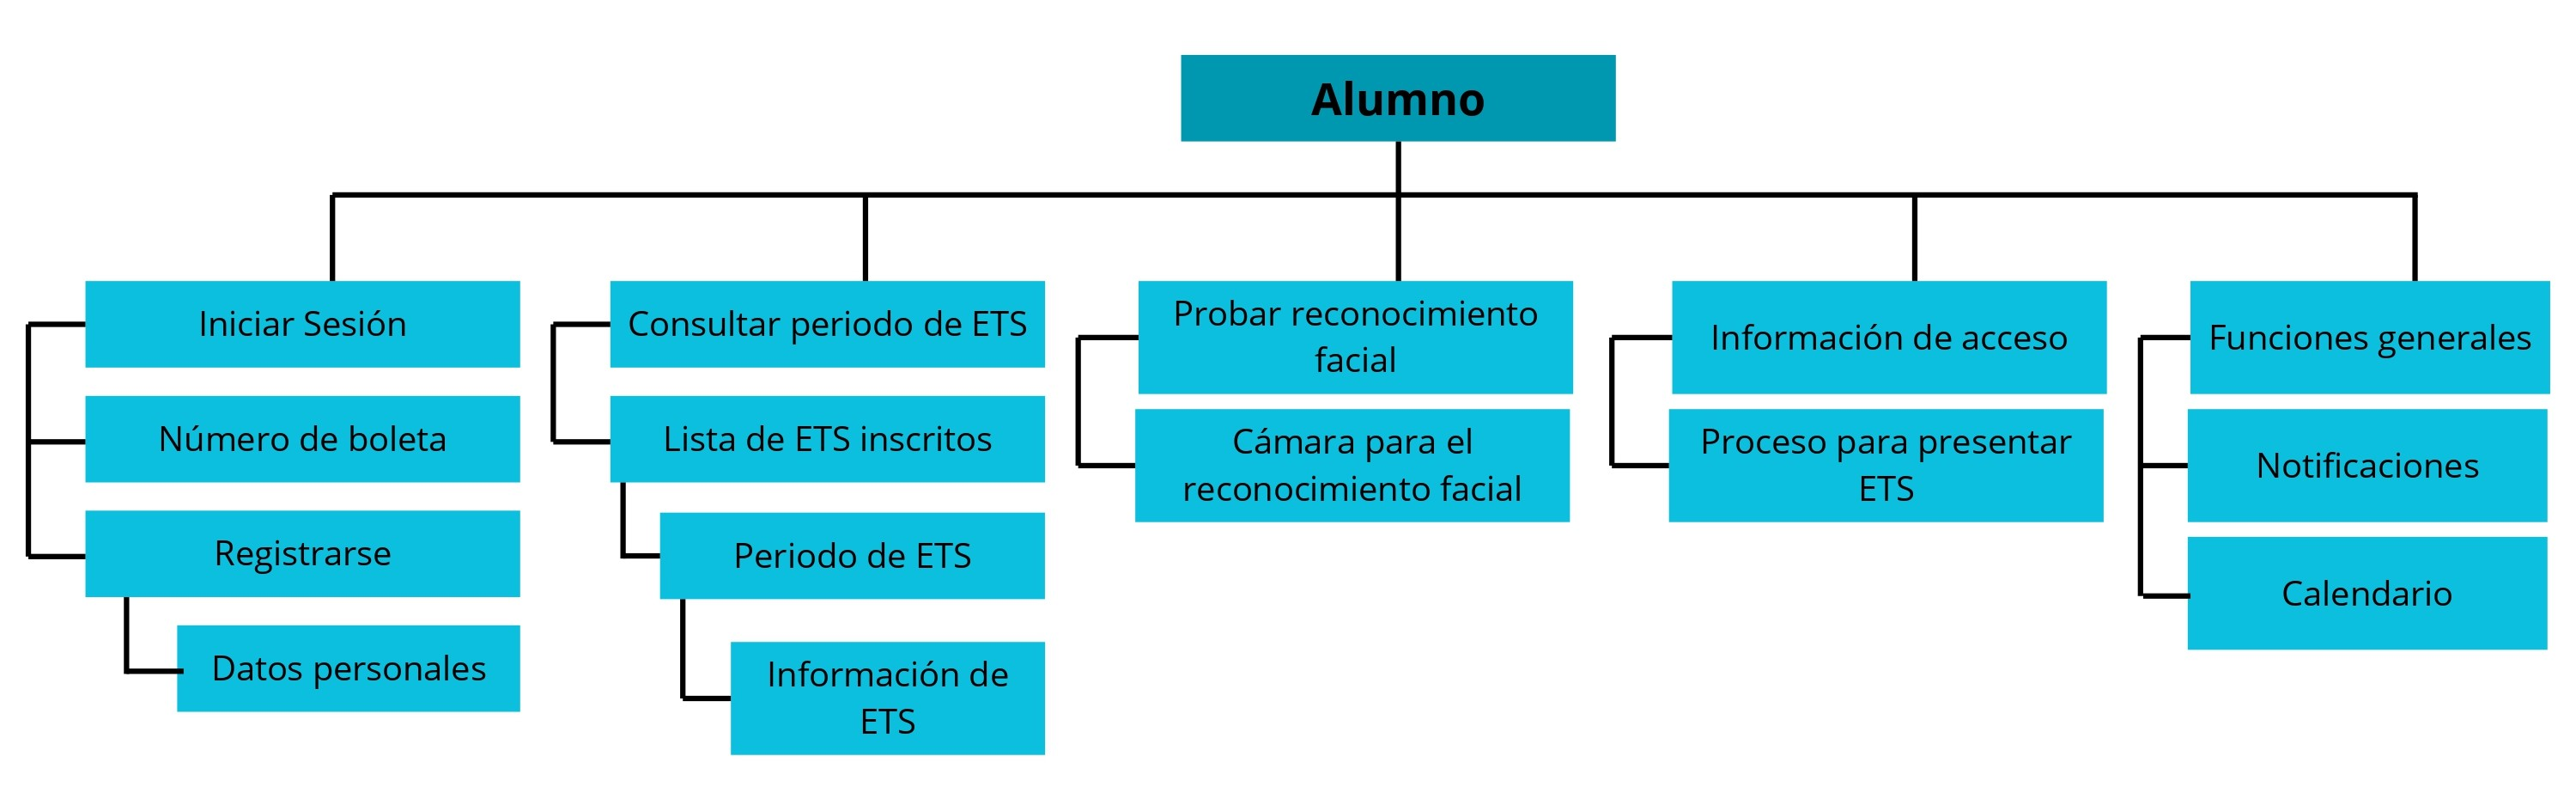
\includegraphics[width=1.0\textwidth]{images/alumno}
			\caption{Mapa de navegación del alumno}
			\label{fig:Mapa de navegación del alumno}
		\end{center}
\end{figure}

\clearpage

\begin{figure}[htbp]
	\begin{center}
		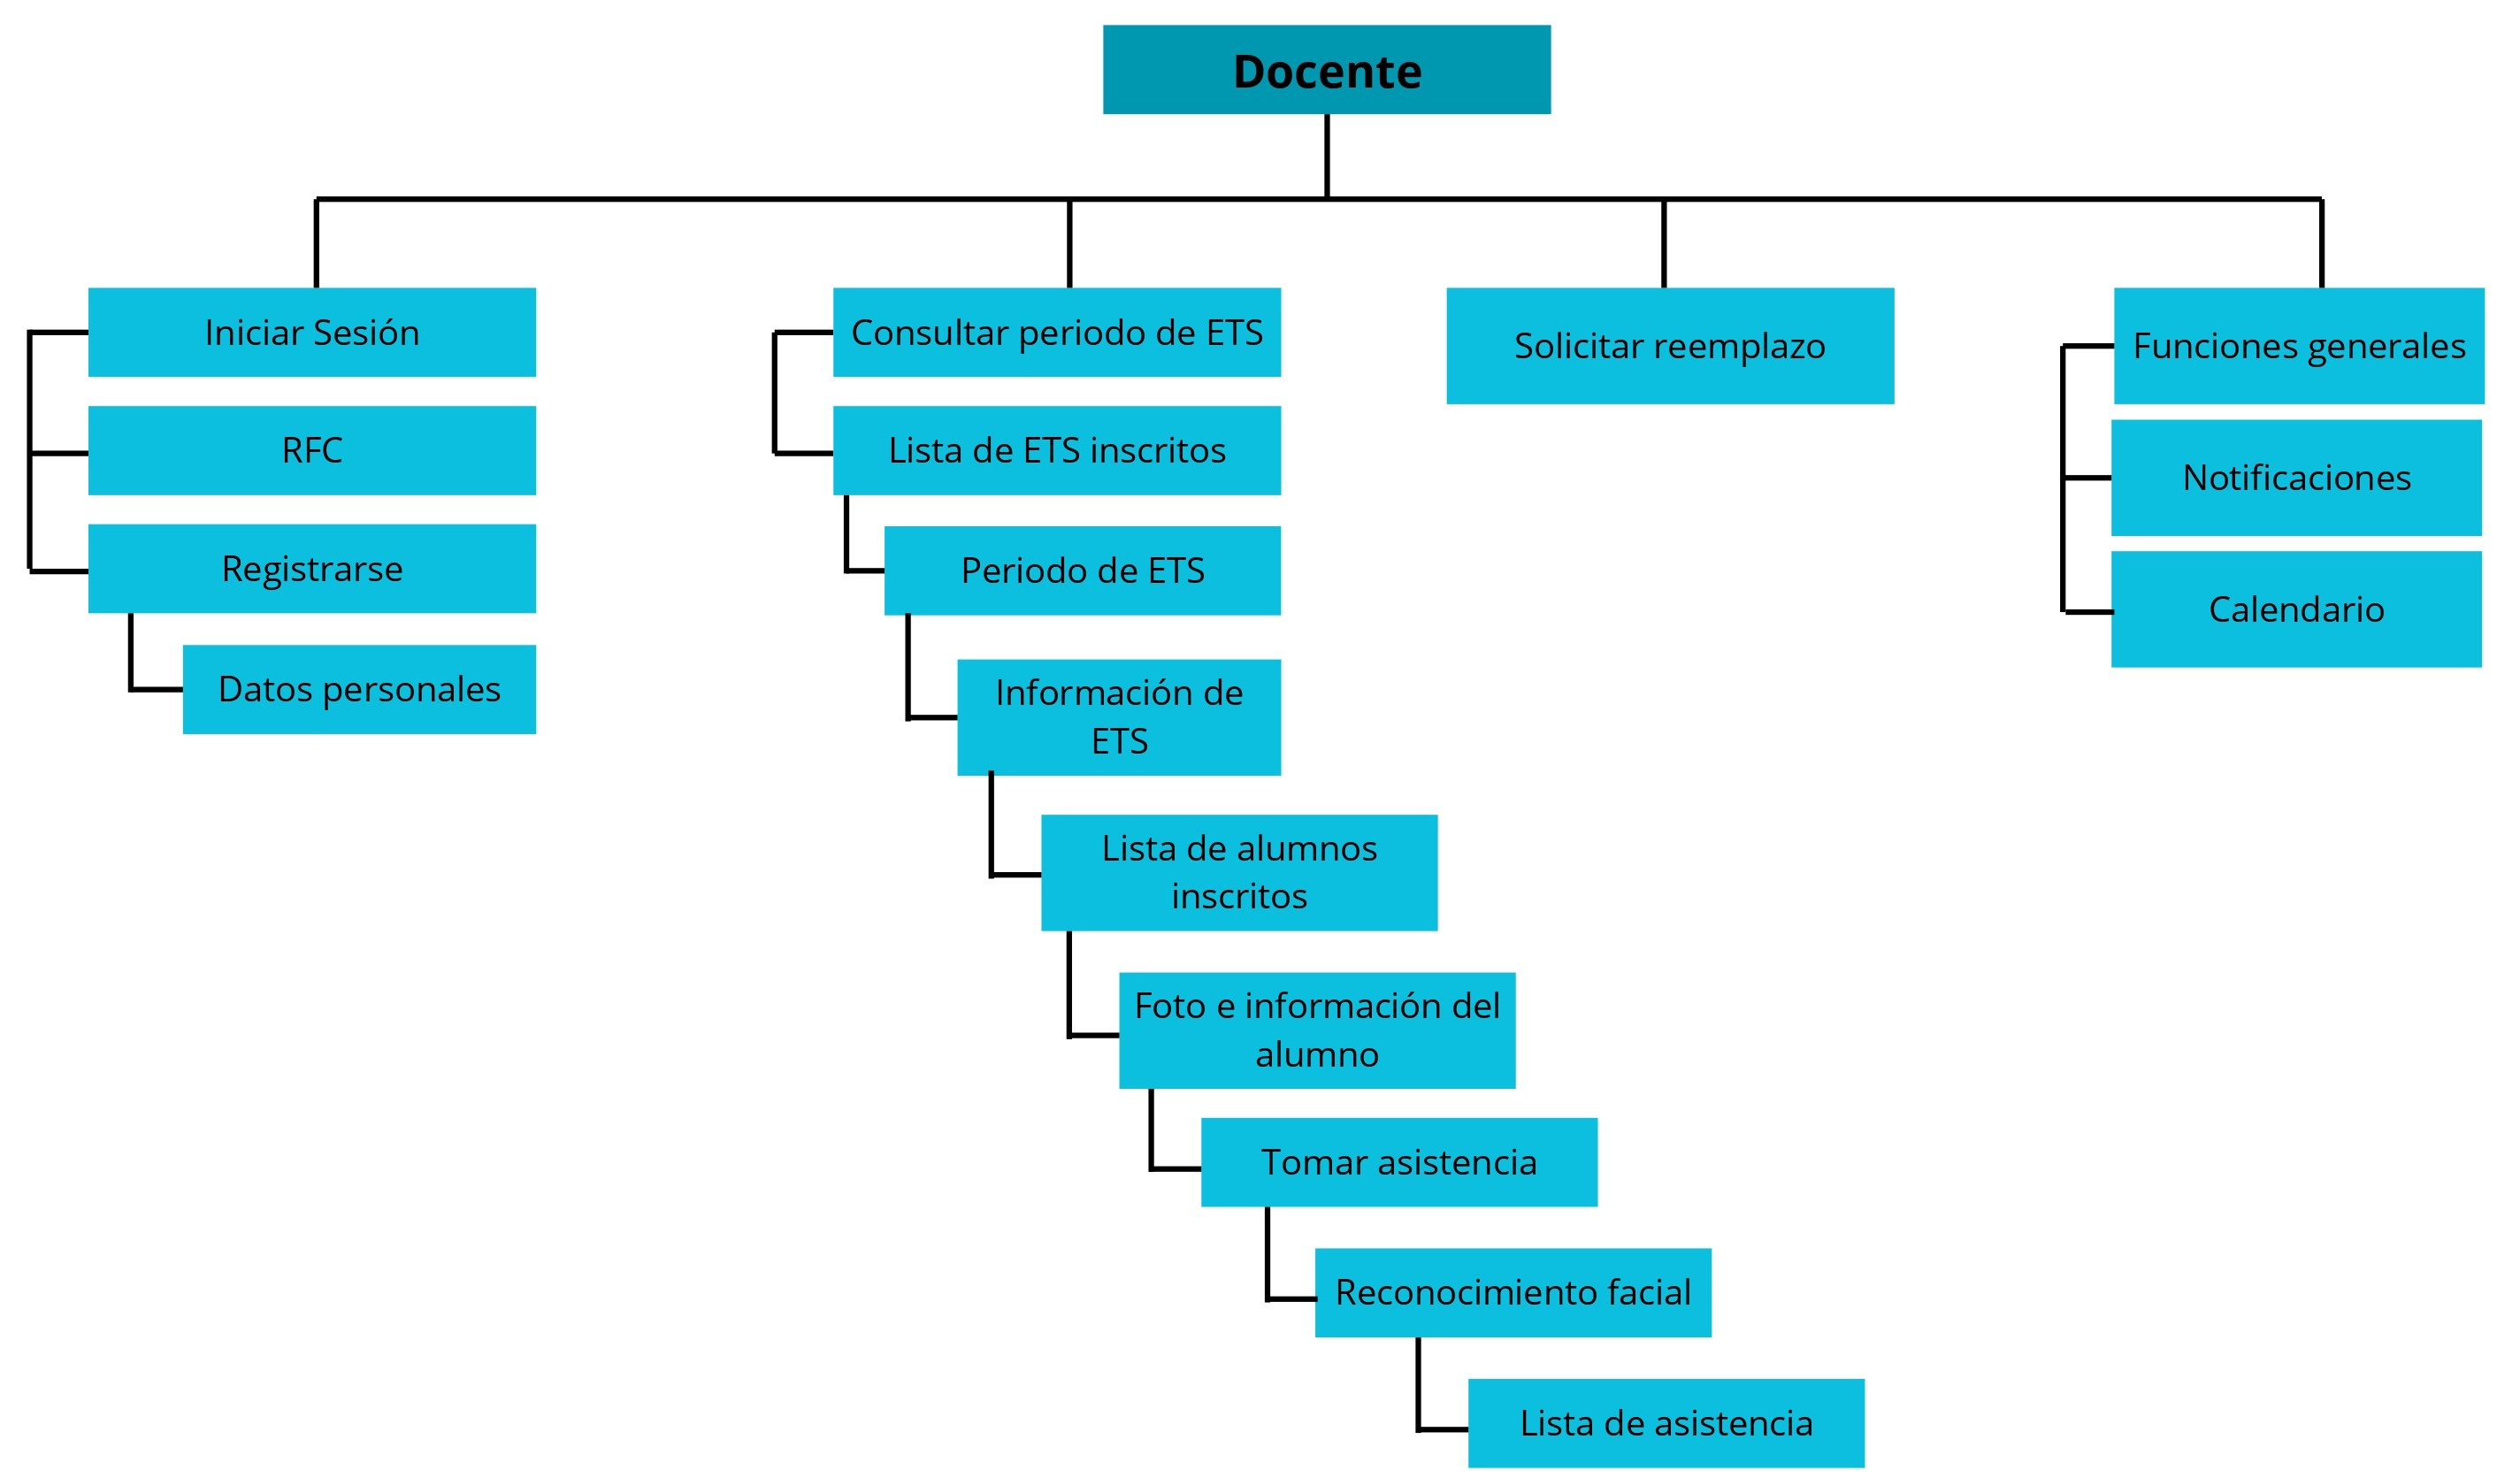
\includegraphics[width=1.0\textwidth]{images/docente}
		\caption{Mapa de navegación del docente}
		\label{fig:Mapa de navegación del docente}
	\end{center}
\end{figure}

\clearpage

\begin{figure}[htbp]
	\begin{center}
		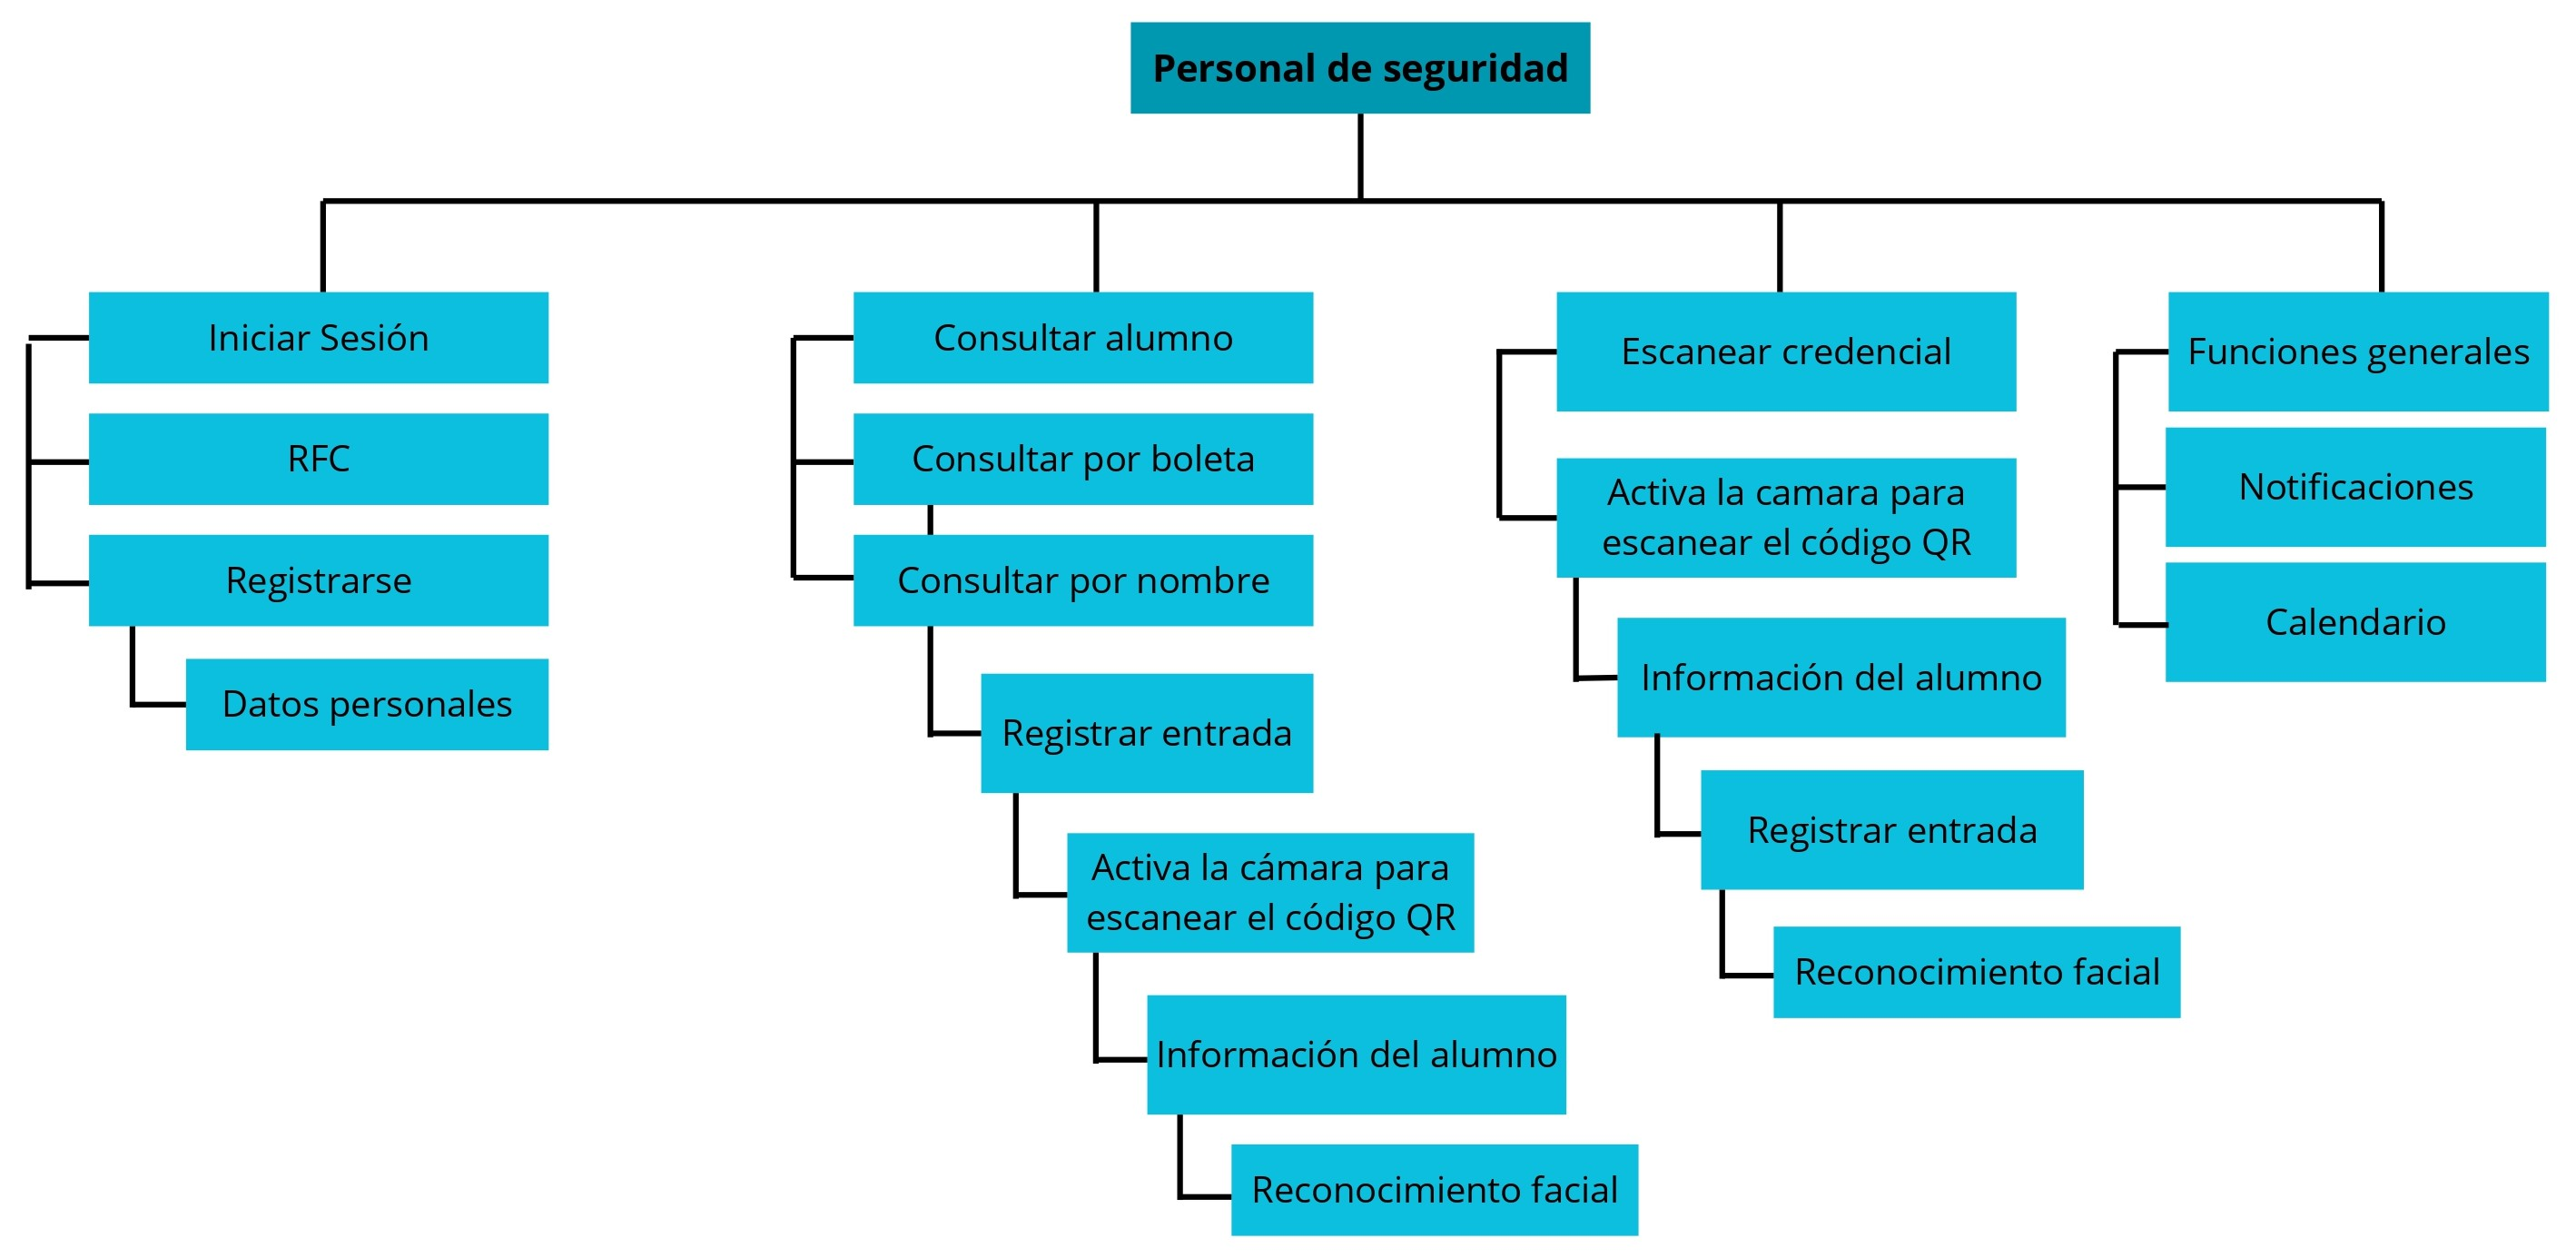
\includegraphics[width=.9\textwidth]{images/personalseguridad}
		\caption{Mapa de navegación del personal de seguridad}
		\label{fig:Mapa de navegación del personal de seguridad}
	\end{center}
\end{figure}

\newpage
% !TeX root = ../ejemplo.tex

%--------------------------------------
\subsection{IU01 Pantalla Iniciar sesión de personal escolar móvil} 

\subsubsection{Objetivo}
	Controlar el acceso al sistema mediante una contraseña a fin de que cada usuario acceda solo a las operaciones permitidas para su perfil.

\subsubsection{Diseño}
	Esta pantalla \IUref{IU01}{Pantalla Iniciar sesión de personal escolar móvil} (ver figura~\ref{IU01}) aparece al iniciar el sistema para los empleados. Para ingresar al mismo se debe escribir el RFC del empleado y la contraseña. 

\IUfig[.35]{UI-CU01}{IU01}{Pantalla Iniciar sesión de personal escolar móvil.}

\subsubsection{Salidas}

Saludo del sistema y mención de su nombre.

\subsubsection{Entradas}
En caso del empleado RFC, Contraseña y en caso del alumno CURP, Contraseña

\subsubsection{Comandos}
\begin{itemize}
	\item \IUbutton{Entrar}: Verifica que el empleado se encuentre registrado y la contraseña sea la correcta. Si la verificación es correcta, se verifica que tipo de empleado y se muestra la pantalla \IUref{IUE01}{Pantalla de Menús de docente} si es docente o \IUref{IUE02}{Pantalla de Menús de personal de seguridad} si es personal de seguridad.
	
	\item \IUbutton{Presiona aquí para pedir su activación}: Redirige a la pantalla \IUref{UI32}{Pantalla de Solicitar desbloqueo de cuenta}
	
\end{itemize}

\subsubsection{Mensajes}

\begin{Citemize}
	\item MSG-1 Los campos no están correctamente llenados. 
	\item MSG-2 Su cuenta esta bloqueada. 
	\item MSG-3 El RFC o la contraseña no corresponden con ningún empleado. 
	\item MSG-4 El proceso no se pudo realizar por un fallo de red. 
	\item MSG-5 Su cuenta ha sido bloqueada por la gran cantidad de intentos de inicio sesión fallidos.
\end{Citemize}


\newpage

% !TeX root = ../ejemplo.tex

%--------------------------------------
\section{IU02 Pantalla Consultar calendario escolar}

\subsection{Objetivo}
Permitir que los usuarios puedan ver el calendario escolar y pedir que se les recuerde cuantos días faltan para que el periodo de ETS comience.
\subsection{Diseño}
    Esta pantalla \IUref{IU02}{Pantalla Consultar calendario escolar} (ver figura~\ref{IU02}) puede ser accedida desde cualquier otra pantalla que no sea el inicio de sesión mediante el botón con forma de calendario.

\IUfig[.35]{UI-CU02}{IU02}{Pantalla Consultar calendario escolar.}

\IUfig[.5]{UI-CU02_2}{IU02-2}{Pantalla Consultar calendario escolar.}

\subsection{Salidas}

    Menciona cuantos días faltan para el periodo de ETS o si menciona que ya es periodo de ETS.

\subsection{Entradas}
   Ninguna.

\subsection{Comandos}
\begin{itemize}
    \item \IUbutton{Calcular cuantos días faltan para el periodo de ETS} toma el día actual y el día de inicio del periodo de ETS más cercano y calcula cuantos días faltan.
    \item \IUbutton{Campana} Redirige a la pantalla \IUref{UI03}{Consultar notificaciones}.
    \item \IUbutton{Home} Redirige a la pantalla de menú correspondiente al tipo de usuario.
\end{itemize}

\subsection{Mensajes}
     
\begin{Citemize}
    \item {\bf MSG7}{``Actualmente es periodo de ETS.''}

    \item {\bf MSG8}{``Actualmente el periodo de ETS no ha sido establecido.''}
\end{Citemize}


\newpage

% !TeX root = ../ejemplo.tex

%--------------------------------------
\section{IU03 Pantalla Consultar notificaciones}

\subsection{Objetivo}
Permitir que los usuarios puedan gestionar sus notificaciones y marcarlas como leidas.
\subsection{Diseño}
    Esta pantalla \IUref{IU03}{Pantalla Consultar notificaciones } (ver figura~\ref{IU03}) puede ser accedida desde cualquier otra pantalla que no sea el inicio de sesión mediante el botón con forma de campana.
\IUfig[.35]{UI-CU03}{IU03}{Pantalla Consultar notificaciones.}

\IUfig[.5]{UI-CU03_2}{IU03-2}{Pantalla Consultar notificaciones.}
\subsection{Salidas}
Menciona que la notificación seleccionada ha sido establecida como leída.
\subsection{Entradas}
   Ninguna.

\subsection{Comandos}
\begin{itemize}
    \item \IUbutton{Botón con palomita} toma la notificación seleccionada y la marca como leída.
    \item \IUbutton{Buscador} En este buscador se puede buscar las notificaciones por fecha.
    \item \IUbutton{Calendario} Redirige a la pantalla \IUref{UI02}{Consultar calendario escolar}
    \item \IUbutton{Home} Redirige a la pantalla de menú correspondiente al tipo de usuario.
\end{itemize}

\subsection{Mensajes}
     
\begin{Citemize}
    \item {\bf MSG9-}{``Actualmente no hay notificaciones.''} 
\end{Citemize}



\newpage

%--------------------------------------
\section{IU04}{Pantalla Periodo de ETS}

\subsection{Objetivo}
	Permitir al docente consultar los periodos de ETS que le han sido asignados. 

\subsection{Diseño}
	Esta pantalla \IUref{IU04}{Pantalla Periodo de ETS} (ver figura~\ref{IU04}) aparece luego de seleccionar la opción de Consultar Periodos de ETS de la pantalla principal. 

\IUfig[.35]{cu04}{IU04}{Pantalla Periodo de ETS.}

\subsection{Salidas}

	Lista de periodos de ETS asignados. 

\subsection{Entradas}
Ninguna

\subsection{Comandos}

\begin{Citemize}
	\item \IUbutton{Calendario} Redirige a la pantalla \IUref{UI02}{Consultar calendario escolar}.
	\item \IUbutton{Campana} Redirige a la pantalla \IUref{UI03}{Consultar notificaciones }.
	\item \IUbutton{Home} Redirige a la pantalla de bienvenida correspondiente al tipo de usuario.
	\item \IUbutton{Periodo de ETS} Selecciona un periodo de ETS y lo redirige a la \IUref{IU04}{pantalla Periodo de ETS}. 
\end{Citemize}


\subsection{Mensajes}

\begin{Citemize}
	\item {\bf MSG-9}{``Error al consultar la base de datos. Intente nuevamente más tarde''.}
	\item {\bf MSG-10}{``No tienes periodos de ETS asignados.''}
\end{Citemize}


\newpage

%--------------------------------------
\section{IU05 Pantalla Consultar ETS}

\subsection{Objetivo}
	Permitir al docente consultar los ETS que tiene asignados. 

\subsection{Diseño}
	Esta pantalla \IUref{IU05}{Pantalla Consultar ETS} (ver figura~\ref{IU05}) aparece luego de seleccionar un periodo de ETS. 

\IUfig[.35]{cu05}{IU05}{Pantalla Consultar ETS.}

\subsection{Salidas}
	Lista de ETS asignados. 

\subsection{Entradas}
	Ninguna
	
\subsection{Comandos}
\begin{Citemize}

	\item \IUbutton{Calendario} Redirige a la pantalla \IUref{UI02}{Consultar calendario escolar}.
	\item \IUbutton{Campana} Redirige a la pantalla \IUref{UI03}{Consultar notificaciones }.
	\item \IUbutton{Home} Redirige a la pantalla de bienvenida correspondiente al tipo de usuario.
	\item \IUbutton{ETS} Selecciona un ETS y lo redirige a la \IUref{IU06}{pantalla Información de ETS}.
\end{Citemize}

\subsection{Mensajes}

\begin{Citemize}
	\item {\bf MSG-9}{``Error al consultar la base de datos. Intente nuevamente más tarde.''.}
	\item {\bf MSG-11}{``No hay ETS asignados actualmente.''}
\end{Citemize}


\newpage

%--------------------------------------
\section{IU06 Pantalla Información de ETS}

\subsection{Objetivo}
	Permitir al docente visualizar la información detallada cada ETS que tiene asignados.
	
\subsection{Diseño}
	Esta pantalla \IUref{IU06}{Pantalla Información de ETS} (ver figura~\ref{IU06}) aparece luego de seleccionar un ETS asignado. 

\IUfig[.35]{cu06}{IU06}{Pantalla Información de ETS}

\subsection{Salidas}

	Información detallada del ETS seleccionado. 

\subsection{Entradas}
Ninguna

\subsection{Comandos}
\begin{itemize}
	\item \IUbutton{Ver alumnos} Redirige a la pantalla \IUref{IU06}{consultar lista de alumnos inscritos a un ETS}
\end{itemize}

\subsection{Mensajes}

\begin{Citemize}
	\item {\bf MSG-12}{``Información no disponible para el ETS seleccionado''}
	\item {\bf MSG-9}{``Error al consultar la base de datos. Intente nuevamente más tarde.''}
\end{Citemize}


\newpage

%--------------------------------------
\section{IU07 Pantalla de Solicitar remplazo}

\subsection{Objetivo}
Permitir al docente pedir que otro docente lo remplaze en la aplicacion de un ETS.

\subsection{Diseño}
Esta pantalla \IUref{IU07}{Pantalla de Solicitar remplazo} (ver figura~\ref{IU07}) aparece luego de que el docente presione el boton \IUbutton{Solicitar docente ayudante} en la pantalla \IUref{IU06}{Pantalla Información de ETS}.

\IUfig[.35]{UI-CU43}{IU07}{Pantalla de Solicitar remplazo}

\subsection{Salidas}
Confirmación de envio de solicitud de remplazo del docente Y y se muestra {\bf MSG-13}{``La notificación ha sido mandada al jefe de departamento y/o al presidente de academia.''}

\subsection{Entradas}
Identificador del ETS y Razon por la que se pide el remplazo.

\subsection{Comandos}
\begin{itemize}
	\item \IUbutton{Enviar}: Permite enviar la notificación al jefe de departamento y/o al presidente de academia para pedir el remplazo.
	\item \IUbutton{Calendario} Redirige a la pantalla \IUref{UI02}{Consultar calendario escolar}.
    \item \IUbutton{Campana} Redirige a la pantalla \IUref{UI03}{Consultar notificaciones }.
    \item \IUbutton{Home} Redirige a la pantalla de bienvenida correspondiente al tipo de usuario.
\end{itemize}

\subsection{Mensajes}

\begin{Citemize}
	\item {\bf MSG-4}{``El proceso no se pudo realizar por un fallo de red.''}
	\item {\bf MSG-13}{``La notificación ha sido mandada al jefe de departamento y/o al presidente de academia.''}
\end{Citemize}


\newpage

%--------------------------------------
\section{IU08 Pantalla Lista de asistencia de ETS}

\subsection{Objetivo}
Permitir al docente visualizar la asistencia de los alumnos inscritos a un ETS asignado.

\subsection{Diseño}
Esta pantalla aparece luego de registrar la asistencia de los alumnos en la \IUref{IU08}{Pantalla lista de asistencia de ETS} (ver figura~\ref{IU08})

\IUfig[.35]{cu08}{IU08}{Pantalla Lista de asistencia de ETS}

\subsection{Salidas}
Lista de asistencia de ETS.

\subsection{Entradas}
Ninguna

\subsection{Comandos}
\begin{itemize}
	\item \IUbutton{Alumno} Selecciona un alumno de la lista para registrar su asistencia y lo redirige a la pantalla \IUref{IU17}{reconocimiento facial}.
	\item \IUbutton{Calendario} Redirige a la pantalla \IUref{UI02}{Consultar calendario escolar}.
    \item \IUbutton{Campana} Redirige a la pantalla \IUref{UI03}{Consultar notificaciones }.
    \item \IUbutton{Home} Redirige a la pantalla de bienvenida correspondiente al tipo de usuario.
\end{itemize}

\subsection{Mensajes}

\begin{Citemize}
	\item {\bf MSG-16}{``No hay alumnos inscritos en este ETS.''}
	\item {\bf MSG-9}{``Error al consultar la base de datos. Intente nuevamente más tarde.''}
	\item {\bf MSG-18}{``Asistencia registrada exitosamente.''}  
\end{Citemize}
\newpage

%--------------------------------------
\subsection{IU09 Asignar docente de remplazo}

\subsubsection{Objetivo}
Permitir al jefe de departamento y/o al presidente de academia responder a las solicitudes de remplazo y asignar un docente de remplazo para el ETS especifico.

\subsubsection{Diseño}
Esta pantalla \IUref{IU09}{Asignar docente de remplazo} (ver figura~\ref{IU09}) aparece luego de que el jefe de departamento y/o al presidente de academia revisen sus notificaciones y seleccione una solicitud de remplazo.

\IUfig[.35]{UI-CU44}{IU09}{Pantalla de Asignar docente de remplazo}

\subsubsection{Salidas}
Confirmación de asignación del nuevo docente y se muestra el mensaje \bf MSG-42{``docente de remplazo asignado con exito.''}.

\subsubsection{Entradas}
Identificador del ETS y nombre del nuevo docente asignado.

\subsubsection{Comandos}
\begin{itemize}
	\item \IUbutton{Asignar}: Permite enviar la notificación docente de que su remplzado ha sido asignado y ademas asigna el remplazo como docente aplicador en el sistema.
\end{itemize}

\subsubsection{Mensajes}

\begin{Citemize}
	\item {\bf MSG-28} {``El proceso no se pudo realizar por un fallo de red''.}
	\item {\bf MSG-42}{``docente de remplazo asignado con exito'.'}
\end{Citemize}



\newpage


%--------------------------------------
\section{IU10 Pantalla Código QR}

\subsection{Objetivo}
Permitir al personal de seguridad escanear el código QR de la credencial del alumno.

\subsection{Diseño}
Esta pantalla \IUref{IU10}{Pantalla Código QR} (ver figura~\ref{IU10}) aparece una vez que el personal de seguridad active la función de escanear credencial del menú. 

\IUfig[.35]{cu12}{IU10}{Pantalla Código QR}

\subsection{Salidas}
Información del alumno

\subsection{Entradas}
Ninguna

\subsection{Comandos}
\begin{itemize}
	\item \IUbutton{Escanear}: Permite escanear el código QR de la credencial del alumno.
	\item \IUbutton{Calendario} Redirige a la pantalla \IUref{UI02}{Consultar calendario escolar}.
    \item \IUbutton{Campana} Redirige a la pantalla \IUref{UI03}{Consultar notificaciones }.
    \item \IUbutton{Home} Redirige a la pantalla de bienvenida correspondiente al tipo de usuario.
\end{itemize}

\subsection{Mensajes}

\begin{Citemize}
	\item {\bf MSG-9}{``Error al consultar la base de datos. Intente nuevamente más tarde.''}.
	\item {\bf MSG-20}{``Alumno no registrado. Verifique el código QR o intente nuevamente.''}
	\item {\bf MSG-19}{``Código QR ilegible. Intente nuevamente.''}
\end{Citemize}


\newpage

%--------------------------------------
\section{IU11}{Pantalla Credencial del alumno}

\subsection{Objetivo}
	Permitir al personal de seguridad consultar la información del alumno mediante el escaneo del código QR de su credencial.

\subsection{Diseño}
Esta pantalla aparece luego de que se escanea el código QR de la credencial del alumno \IUref{IU11}{Pantalla Credencial del alumno} (ver figura~\ref{IU11}).
	

\IUfig[.35]{cu14}{IU11}{Pantalla Credencial del alumno}

\subsection{Salidas}
	Información del alumno

\subsection{Entradas}
Ninguna

\subsection{Comandos}
\begin{itemize}
	\item \IUbutton{Registrar asistencia}: Permite registrar la asistencia del alumno.
	\item \IUbutton{Calendario} Redirige a la pantalla \IUref{UI02}{Consultar calendario escolar}.
    \item \IUbutton{Campana} Redirige a la pantalla \IUref{UI03}{Consultar notificaciones }.
    \item \IUbutton{Home} Redirige a la pantalla de bienvenida correspondiente al tipo de usuario.
\end{itemize}

\subsection{Mensajes}

\begin{Citemize}
	\item {\bf MSG-20}{``Alumno no registrado''}
	\item {\bf MSG-11}{``Error al consultar la base de datos. Intente nuevamente más tarde.''}
\end{Citemize}


\newpage

%--------------------------------------
\section{IU12-1 Pantalla Buscar alumno por boleta}

\subsection{Objetivo}
	Permitir al personal de seguridad buscar la información de un alumno utilizando su numero de boleta. 

\subsection{Diseño}
	Esta pantalla \IUref{IU12}{Pantalla Buscar alumno} (ver figura~\ref{IU12}) aparece luego de seleccionar la opción Consultar alumno. 

\IUfig[.35]{cu11}{IU12}{Pantalla Buscar alumno.}

\subsection{Salidas}
	Información del alumno.

\subsection{Entradas}
Número de boleta del alumno. 

\subsection{Comandos}
Buscador: Permite al usuario buscar al alumno ingresando su numero de boleta. 

\subsection{Mensajes}

\begin{Citemize}
	\item {\bf MSG-20-}{``Alumno no registrado''}
\end{Citemize}


\newpage

%%--------------------------------------
\section{IU12-2 Pantalla Buscar alumno por nombre}

\subsection{Objetivo}
Permitir al personal de seguridad buscar la información de un alumno utilizando su nombre. 

\subsection{Diseño}
Esta pantalla \IUref{IU12}{Pantalla Buscar alumno} aparece luego de seleccionar la opción Consultar alumno. 

\IUfig[.35]{cu11}{IU12}{Pantalla Buscar alumno.}

\subsection{Salidas}
Información del alumno.

\subsection{Entradas}
Nombre del alumno. 

\subsection{Comandos}

\begin{itemize}

	\item Buscador: Permite al usuario buscar al alumno ingresando su nombre. 
	\item \IUbutton{Calendario} Redirige a la pantalla \IUref{UI02}{Consultar calendario escolar}.
    \item \IUbutton{Campana} Redirige a la pantalla \IUref{UI03}{Consultar notificaciones }.
    \item \IUbutton{Home} Redirige a la pantalla de bienvenida correspondiente al tipo de usuario.
\end{itemize}

\subsection{Mensajes}

\begin{Citemize}
	\item {\bf MSG-20}{``Alumno no registrado''}
\end{Citemize}



%\newpage

%--------------------------------------
\subsection{IU13 Pantalla consultar lista de alumnos inscritos a un ETS}

\subsubsection{Objetivo}
Permitir al docente visualizar la lista de los alumnos inscritos a un ETS asignado.

\subsubsection{Diseño}
Esta pantalla aparece luego de seleccionar un ETS en la \IUref{IU13}{Pantalla Informacion de ETS} (ver figura~\ref{IU06} y muestra la boleta, el nombre completo y la foto de los alumnos inscritos al ETS)

\IUfig[.35]{cu07}{IU13}{Consultar lista de alumnos inscritos a un ETS}

\subsubsection{Salidas}
Lista de los alumnos inscritos al ETS.

\subsubsection{Entradas}
Ninguna

\subsubsection{Comandos}
\begin{itemize}
    \item \IUbutton{Calendario} Redirige a la pantalla \IUref{UI02}{Consultar calendario escolar}.
    \item \IUbutton{Campana} Redirige a la pantalla \IUref{UI03}{Consultar notificaciones }.
    \item \IUbutton{Home} Redirige a la pantalla de bienvenida correspondiente al tipo de usuario.
	\item \IUbutton{Tomar asistencia} redirige a la pantalla \IUref{IU08}{Lista de asistencia de ETS}.
\end{itemize}

\subsubsection{Mensajes}

\begin{Citemize}
	\item {\bf MSG-14}{``No hay alumnos inscritos en este ETS.''}
	\item {\bf MSG9-}{``Error al consultar la base de datos. Intente nuevamente más tarde.''}. 
\end{Citemize}
\newpage

%--------------------------------------
\section{IU14} {Pantalla Periodo de ETS del alumno}

\subsection{Objetivo}
	Permitir al alumno consultar los periodos de ETS que le han sido asignados. 

\subsection{Diseño}
	Esta pantalla \IUref{IU14}{Pantalla Periodo de ETS del alumno} (ver figura~\ref{IU14}) aparece luego de seleccionar la opción de Consultar Periodos.

\IUfig[.35]{cu16}{IU14}{Pantalla Periodo de ETS del alumno.}

\subsection{Salidas}
	Lista de periodos de ETS. 

\subsection{Entradas}
Ninguna

\subsection{Comandos}

\begin{itemize}
	\item \IUbutton{Calendario} Redirige a la pantalla \IUref{UI02}{Consultar calendario escolar}.
	\item \IUbutton{Campana} Redirige a la pantalla \IUref{UI03}{Consultar notificaciones }.
	\item \IUbutton{Home} Redirige a la pantalla de bienvenida correspondiente al tipo de usuario.
	\item \IUbutton{Periodo de ETS} Selecciona un periodo de ETS y lo redirige a la pantalla \IUref{UI15}{consultar ETS del alumno}.
\end{itemize}

\subsection{Mensajes}

\begin{Citemize}
	\item {\bf MSG-25}{``No hay periodos de ETS''}
	\item {\bf MSG-9}{``Error al consultar la base de datos. Intente nuevamente más tarde.''}
\end{Citemize}


\newpage

%--------------------------------------
\section{IU15} {Pantalla Consultar ETS del alumno}

\subsection{Objetivo}
Permitir al alumno consultar los ETS que tiene inscritos. 

\subsection{Diseño}
Esta pantalla \IUref{IU15}{Pantalla Consultar ETS del alumno} (ver figura~\ref{IU15}) aparece luego de seleccionar un periodo de ETS. 

\IUfig[.35]{cu17}{IU15}{Pantalla Consultar ETS del alumno.}

\subsection{Salidas}
Lista de ETS asignados. 

\subsection{Entradas}
Ninguna


\subsection{Comandos}

\begin{itemize}
	\item \IUbutton{Calendario} Redirige a la pantalla \IUref{UI02}{Consultar calendario escolar}.
	\item \IUbutton{Campana} Redirige a la pantalla \IUref{UI03}{Consultar notificaciones }.
	\item \IUbutton{Home} Redirige a la pantalla de bienvenida correspondiente al tipo de usuario.
\end{itemize}
\subsection{Mensajes}

\begin{Citemize}
	\item {\bf MSG-26}{``No hay ETS inscritos actualmente.''}
	\item {\bf MSG-09}{``Error al consultar la base de datos. Intente nuevamente más tarde.''}
\end{Citemize}

\newpage

%%--------------------------------------
\section{IU15} {Pantalla Consultar ETS del alumno}

\subsection{Objetivo}
Permitir al alumno consultar los ETS que tiene inscritos. 

\subsection{Diseño}
Esta pantalla \IUref{IU15}{Pantalla Consultar ETS del alumno} (ver figura~\ref{IU15}) aparece luego de seleccionar un periodo de ETS. 

\IUfig[.35]{cu17}{IU15}{Pantalla Consultar ETS del alumno.}

\subsection{Salidas}
Lista de ETS asignados. 

\subsection{Entradas}
Ninguna


\subsection{Comandos}

\begin{itemize}
	\item \IUbutton{Calendario} Redirige a la pantalla \IUref{UI02}{Consultar calendario escolar}.
	\item \IUbutton{Campana} Redirige a la pantalla \IUref{UI03}{Consultar notificaciones }.
	\item \IUbutton{Home} Redirige a la pantalla de bienvenida correspondiente al tipo de usuario.
\end{itemize}
\subsection{Mensajes}

\begin{Citemize}
	\item {\bf MSG-26}{``No hay ETS inscritos actualmente.''}
	\item {\bf MSG-09}{``Error al consultar la base de datos. Intente nuevamente más tarde.''}
\end{Citemize}

%--------------------------------------
\section{IU16 Pantalla Información de ETS}

\subsection{Objetivo}
Permitir al alumno visualizar la información detallada cada ETS que tiene inscrito.

\subsection{Diseño}
Esta pantalla \IUref{IU16}{Pantalla de Información de ETS del alumno} (ver figura~\ref{IU16}) aparece luego de seleccionar un ETS inscrito. 

\IUfig[.35]{cu18}{IU16}{Pantalla de Información de ETS del alumno}

\subsection{Salidas}

Información detallada del ETS seleccionado. 

\subsection{Entradas}
Ninguna


\subsection{Comandos}
\begin{itemize}
	\item \IUbutton{Calendario} Redirige a la pantalla \IUref{UI02}{Consultar calendario escolar}.
    \item \IUbutton{Campana} Redirige a la pantalla \IUref{UI03}{Consultar notificaciones }.
    \item \IUbutton{Home} Redirige a la pantalla de bienvenida correspondiente al tipo de usuario.
\end{itemize}

\subsection{Mensajes}

\begin{Citemize}
	\item {\bf MSG-13}{``Información no disponible para el ETS seleccinado''}
	\item {\bf MSG-11}{``Error al consultar la base de datos. Intente nuevamente más tarde.''}
\end{Citemize}



\newpage

%--------------------------------------
\section{IU17 Pantalla de Reconocimiento facial}

\subsection{Objetivo}
Permitir al docente registrar la asistencia al ETS de los alumnos y al personal de seguridad le permite registrar la entrada a las instalaciones.

\subsection{Diseño}
Esta pantalla \IUref{IU17}{Pantalla de Reconocimiento facial} (ver figura~\ref{IU17}) aparece luego de seleccionar el botón \IUbutton{Registrar asistencia} desde la pantalla \IUref{IU08}{Lista de asistencia de ETS}..


\IUfig[.30]{cu19}{IU17}{Pantalla de Reconocimiento facial}

\subsection{Salidas}
Confirmación de asistencia registrada

\subsection{Entradas}
Ninguna

\subsection{Comandos}
\begin{itemize}
    \item \IUbutton{Cancelar}: Permite al alumno cancelar la operación de Reconocimeinto facial.
    \item \IUbutton{Comenzar}: Activa la cámara para el Reconocimiento facil. 
    \item \IUbutton{Calendario} Redirige a la pantalla \IUref{UI02}{Consultar calendario escolar}.
    \item \IUbutton{Campana} Redirige a la pantalla \IUref{UI03}{Consultar notificaciones }.
    \item \IUbutton{Home} Redirige a la pantalla de bienvenida correspondiente al tipo de usuario.
    \item \IUbutton{Registrar asistencia} Si el usuario que presiona el botón es un docente, marca la asistencia del alumno al ETS, por otro lado si el usuario que presiona es un botón personal de seguridad, marca la entrada del alumno a las instalaciones.
    \item \IUbutton{No registrar asistencia} No marca la asistencia ni la entrada (El alumno no es quien dice ser).
\end{itemize}

\subsection{Mensajes}

\begin{Citemize}
    \item {\bf MSG-17}{``No se pudo activar la cámara o reconocer la identidad. Intente nuevamente.''}
    \item {\bf MSG-16}{``No hay alumnos inscritos en este ETS.''}
    \item {\bf MSG-9}{``Error al consultar la base de datos. Intente nuevamente más tarde.''}
    \item {\bf MSG-15}{``Asistencia registrada exitosamente.''}
    \item {\bf MSG-23}{``Entrada registrada exitosamente.''}
    \item {\bf MSG-24}{``Entrada no registrada .''}
\end{Citemize}

\newpage

%--------------------------------------
\subsection{IU18 Pantalla de Detalles del proceso de ETS}

\subsubsection{Objetivo}
Permitir al alumno visualizar la información detallada sobre el proceso de ETS.

\subsubsection{Diseño}
Esta pantalla \IUref{IU18}{Pantalla de Detalles del proceso de ETS} (ver figura~\ref{IU18}) aparece luego de seleccionar el botón \IUbutton{Revisar Información de acceso}. 

\IUfig[.35]{CU20}{IU18}{Pantalla de Detalles del proces de ETS}

\subsubsection{Salidas}

Información detallada del proceso de ETS. 

\subsubsection{Entradas}
Ninguna


\subsubsection{Comandos}
\begin{itemize}
	\item \IUbutton{Calendario} Redirige a la pantalla \IUref{UI02}{Consultar calendario escolar}.
	\item \IUbutton{Campana} Redirige a la pantalla \IUref{UI03}{Consultar notificaciones }.
	\item \IUbutton{Home} Redirige a la pantalla de bienvenida correspondiente al tipo de usuario.
\end{itemize}
\subsubsection{Mensajes}

\begin{Citemize}
	\item {\bf MSG-9}{``Error al querer mostrar la información. Por favor, intente nuevamente.''}
\end{Citemize}


\newpage

\section{IU19 Pantalla de Reconocimiento facial alumno}

\subsection{Objetivo}
Permitir al alumno probar el reconocimiento facial.

\subsection{Diseño}
Esta pantalla \IUref{IU19}{Pantalla de Reconocimiento facial alumno} (ver figura~\ref{IU19}) aparece luego de seleccionar el botón \IUbutton{Probar reconocimiento facial} en la pantalla \IUref{IU16}{Pantalla de Información de ETS del alumno}.

\IUfig[.35]{cu19-2}{IU19}{Pantalla de Reconocimiento facial}

\subsection{Salidas}
Confirmación de que el reconocimiento facial funciona con el alumno.

\subsection{Entradas}
Ninguna

\subsection{Comandos}
\begin{itemize}
    \item \IUbutton{Cancelar}: Permite al alumno cancelar la operación de Reconocimeinto facial.
    \item \IUbutton{Comenzar}: Activa la cámara para el Reconocimiento facil. 
    \item \IUbutton{Calendario} Redirige a la pantalla \IUref{UI02}{Consultar calendario escolar}.
    \item \IUbutton{Campana} Redirige a la pantalla \IUref{UI03}{Consultar notificaciones }.
    \item \IUbutton{Home} Redirige a la pantalla de bienvenida correspondiente al tipo de usuario.
\end{itemize}

\subsection{Mensajes}

\begin{Citemize}
    \item {\bf MSG-17}{``No se pudo activar la cámara o reconocer la identidad. Intente nuevamente.''}
    \item {\bf MSG-16}{``No hay alumnos inscritos en este ETS.''}
    \item {\bf MSG-9}{``Error al consultar la base de datos. Intente nuevamente más tarde.''}
\end{Citemize}
\newpage

%--------------------------------------
\section{IU20}{Mostrar la foto e información  del alumno}

\subsection{Objetivo}
    Mostrar la al docente la información del alumno seleccionado.

\subsection{Diseño}
    Esta \IUref{IU20}{Pantalla mostrar la foto e información  del alumno} (ver figura~\ref{IU20}) muestra toda la información que necesita al docente para poder reconocerlo.

\IUfig[.35]{cu11}{IU20}{Pantalla mostrar la foto e información  del alumno.}

\subsection{Salidas}

    Ninguna.

\subsection{Entradas}
    Ninguna.

\subsection{Comandos}
\begin{itemize}
    \item \IUbutton{Ampliar fotografía}: Muestra la fotografía del alumno ampliada. 
    
\end{itemize}

\subsection{Mensajes}

\begin{Citemize}
    \item {\bf MSG4-} ``El proceso no se pudo realizar por un falló de red.''
\end{Citemize}


\newpage

% !TeX root = ../ejemplo.tex

%--------------------------------------
\subsection{IU21 Dar de alta a alumno}

\subsubsection{Objetivo}
	Permitir al personal de la DAE dar de alta a un alumno.
\subsubsection{Diseño}
    Esta pantalla \IUref{IU21}{ Dar de alta a alumno } (ver figura~\ref{IU21}) puede ser accedida desde la pantalla \IUref{IUE04}{de personal de la DAE}

\IUfig[1]{UI-CU21}{IU21}{ Dar de alta a alumno.}

\subsubsection{Salidas}
Muestra mensaje {\bf MSG-31} ``Alumno dado de alta con éxito''.
\subsubsection{Entradas}
    \hyperlink{Alumno.Boleta}{Boleta}, \hyperlink{Alumno.Nombre}{Nombre}, \hyperlink{Alumno.CURP}{CURP}, \hyperlink{Alumno.Sexo}{Sexo} y \hyperlink{Alumno.Correo institucional}{Correo institucional}
\subsubsection{Comandos}
\begin{itemize}
    \item \IUbutton{Dar de alta un alumno}  El sistema revisa que los datos del alumno sean válidos, verifica que el CURP o la boleta no hayan sido registrados con anterioridad, mantiene los datos para usarlos en el proceso de crear credencial. Y redirige a la pantalla \IUref{UI22}{Crear credencial}.
    \item \IUbutton{Calendario} Redirige a la pantalla \IUref{UI02}{Consultar calendario escolar}.
    \item \IUbutton{Campana} Redirige a la pantalla \IUref{UI03}{Consultar notificaciones }.
    \item \IUbutton{Home} Redirige a la pantalla de bienvenida correspondiente al tipo de usuario.
    
\end{itemize}

\subsubsection{Mensajes}

\begin{Citemize}
    \item {\bf MSG-31} ``Alumno dado de alta con éxito''.
    \item {\bf MSG-28}  ``El proceso no se pudo realizar por un falló de red.''
    \item {\bf MSG-29}{``Los campos no están correctamente llenados.''}
    \item {\bf MSG-30}{``La CURP o la boleta ya han sido asociadas a este alumno con anterioridad u otro alumno.''}
\end{Citemize}

\newpage

% !TeX root = ../ejemplo.tex

%--------------------------------------
\subsection{IU22 Crear credencial}

\subsubsection{Objetivo}
   Permite al personal de gestión escolar revisar una previsualización de la credencial del alumno y revisar los datos.
\subsubsection{Diseño}
    Esta pantalla \IUref{IU22}{ Crear credencial } (ver figura~\ref{IU22}) puede ser accedida desde la pantalla \IUref{IU21}{ Dar de alta a alumno} apretando el botón \IUbutton{Dar de alta alumno }.

\IUfig[1]{UI-CU22}{IU22}{ Crear credencial.}

\subsubsection{Salidas}
Ninguna
\subsubsection{Entradas}
    \hyperlink{Alumno.Boleta}{Boleta}, \hyperlink{Alumno.Nombre}{Nombre}, \hyperlink{Alumno.CURP}{CURP}, \hyperlink{Alumno.Sexo}{Sexo} y \hyperlink{Alumno.Correo institucional}{Correo institucional}
\subsubsection{Comandos}
\begin{itemize}
\item \IUbutton{Subir foto} Guarda la información y redirige a la pantalla \IUref{UI23}{ Capturar fotografía estudiantil }.
    \item \IUbutton{Home} Redirige a la pantalla de bienvenida correspondiente al tipo de usuario.
    
\end{itemize}

\subsubsection{Mensajes}

\begin{Citemize}
    \item {\bf MSG-28}  ``El proceso no se pudo realizar por un falló de red.''
    \item {\bf MSG-29}{``Los campos no están correctamente llenados.''}
    \item {\bf MSG-30}{``El CURP o la boleta ya han sido asociadas a este alumno con anterioridad u otro alumno.''}
\end{Citemize}

\newpage

% !TeX root = ../ejemplo.tex

%--------------------------------------
\subsection{IU23 Capturar fotografía estudiantil}

\subsubsection{Objetivo}
   Permite agregar una foto a la credencial, para su posterior registro, además de obtener 5 fotos para ser guardadas en la base de datos.
\subsubsection{Diseño}
    Esta pantalla \IUref{IU23}{ Capturar fotografía estudiantil} (ver figura~\ref{IU23}) puede ser accedida desde la pantalla \IUref{IU22}{ Crear credencial} apretando el botón \IUbutton{Subir foto}

\IUfig[1]{UI-CU23}{IU23}{ Capturar fotografía estudiantil.}

\subsubsection{Salidas}
Ninguna
\subsubsection{Entradas}
Ninguna
\subsubsection{Comandos}
\begin{itemize}
    \item \IUbutton{Cámara} Toma 5 fotos al alumno, las cuales guarda en la base de datos para el sistema de reconocimiento facial, de estas la primera la usa para la credencial y redirige a la pantalla \IUref{UI21}{ Capturar fotografía estudiantil }.
    \item \IUbutton{Calendario} Redirige a la pantalla \IUref{UI02}{Consultar calendario escolar}.
    \item \IUbutton{Campana} Redirige a la pantalla \IUref{UI03}{Consultar notificaciones }.
    \item \IUbutton{Home} Redirige a la pantalla de bienvenida correspondiente al tipo de usuario.
    
\end{itemize}

\subsubsection{Mensajes}

\begin{Citemize}
    \item {\bf MSG-28}  ``El proceso no se pudo realizar por un fallo de red.''
\end{Citemize}


\newpage

% !TeX root = ../ejemplo.tex

%--------------------------------------
\section{IU24}{Consultar lista de periodo de ETS}
\subsection{Objetivo}
   Permite al personal de gestión escolar consultar una lista con todos los periodos de ETS y el periodo de ETS más actual en la parte superior.
\subsection{Diseño}
    Esta pantalla \IUref{IU24}{ Consultar lista de periodo de ETS } (ver figura~\ref{IU24}) puede ser accedida desde la pantalla \IUref{IUE05}{de saludo de gestión escolar } apretando el botón \IUbutton{Consultar lista de periodo de ETS}
\IUfig[1]{UI-CU24}{IU24}{ Consultar lista de periodo de ETS.}

\subsection{Salidas}
Ninguna
\subsection{Entradas}
Ninguna
\subsection{Comandos}
\begin{itemize}
    \item \IUbutton{ Dar de alta periodo de ETS } Redirige a la pantalla \IUref{UI25}{ Dar de alta de periodo de ETS}.
    \item \IUbutton{Calendario} Redirige a la pantalla \IUref{UI02}{Consultar calendario escolar}.
    \item \IUbutton{Campana} Redirige a la pantalla \IUref{UI03}{Consultar notificaciones }.
    \item \IUbutton{Home} Redirige a la pantalla de bienvenida correspondiente al tipo de usuario.
    
\end{itemize}

\subsection{Mensajes}

\begin{Citemize}
    \item {\bf MSG-28}  ``El proceso no se pudo realizar por un fallo de red.''
    \item {\bf MSG-31}  ``Ningún periodo de ETS ha sido dado de alta.''
\end{Citemize}



\newpage

% !TeX root = ../ejemplo.tex

%--------------------------------------
\section{IU25 Dar de alta de periodo de ETS}
\subsection{Objetivo}
    Permite al personal de gestión escolar dar de alta un periodo de ETS.
\subsection{Diseño}
    Esta pantalla \IUref{IU25}{Dar de alta de periodo de ETS } (ver figura~\ref{IU25}) puede ser accedida desde la pantalla \IUref{IU24}{Consultar lista de periodo de ETS}
\IUfig[.35]{UI-CU25}{IU25}{Dar de alta de periodo de ETS.}

\subsection{Salidas}
Muestra mensaje {\bf MSG15-} ``Periodo de ETS  dado de alta con éxito''.
\subsection{Entradas}
\hyperlink{Periodo de ETS.Periodo}{Periodo}, \hyperlink{Periodo-de-ETS.Tipo}{Tipo}, \hyperlink{Periodo-de-ETS.Fecha-de-inicio}{Fecha-de-inicio} y \hyperlink{Periodo-de-ETS.Fecha-de-fin}{Fecha-de-fin}
\subsection{Comandos}
\begin{itemize}
    \item \IUbutton{Dar de alta periodo de ETS} Da de alta el nuevo periodo de ETS y redirige a la pantalla \IUref{UI24}{ Consultar lista de periodo de ETS}.
    \item \IUbutton{Calendario} Redirige a la pantalla \IUref{UI02}{Consultar calendario escolar}.
    \item \IUbutton{Campana} Redirige a la pantalla \IUref{UI03}{Consultar notificaciones }.
    \item \IUbutton{Home} Redirige a la pantalla de menú correspondiente al tipo de usuario.
    
\end{itemize}

\subsection{Mensajes}

\begin{Citemize}
    \item {\bf MSG15-} ``Periodo de ETS  dado de alta con éxito''.
    \item {\bf MSG4-}  ``El proceso no se pudo realizar por un fallo de red.''
    \item {\bf MSG1-}{``Los campos no están correctamente llenados.''}
    \item {\bf MSG16-}{`` Periodo, Fecha-de-inicio o Fecha-de-fin ya han sido asociadas a un periodo de ETS.''}
\end{Citemize}


\newpage

% !TeX root = ../ejemplo.tex

%--------------------------------------
\subsection{IU26 Consultar lista de ETS}
\subsubsection{Objetivo}
    Permite al personal de gestión escolar consultar una lista con todos ETS.
\subsubsection{Diseño}
    Esta pantalla \IUref{IU26}{Consultar lista de ETS} (ver figura~\ref{IU26}) puede ser accedida desde la pantalla \IUref{IUE05}{ de saludo de gestión escolar } apretando el botón \IUbutton{Consultar lista de ETS}
\IUfig[]{UI-CU28}{IU26}{Consultar lista ETS.}

\subsubsection{Salidas}
Ninguna
\subsubsection{Entradas}
Ninguna
\subsubsection{Comandos}
\begin{itemize}
    \item \IUbutton{Dar de alta un ETS} Redirige a la pantalla \IUref{UI27}{ Dar de alta ETS}.
    \item \IUbutton{Home} Redirige a la pantalla de bienvenida correspondiente al tipo de usuario.
    
\end{itemize}

\subsubsection{Mensajes}

\begin{Citemize}
    \item {\bf MSG-28}  ``El proceso no se pudo realizar por un fallo de red.''
    \item {\bf MSG-34}  ``Ningún ETS ha sido dado da alta.''
\end{Citemize}


\newpage

% !TeX root = ../ejemplo.tex

%--------------------------------------
\subsection{IU27 Dar de alta ETS}
\subsubsection{Objetivo}
    Permite al personal de gestión escolar dar de alta un ETS.
\subsubsection{Diseño}
    Esta pantalla \IUref{IU27}{Dar de alta ETS} (ver figura~\ref{IU27}) puede ser accedida desde la pantalla \IUref{IU26}{Consultar lista de ETS} apretando el botón \IUbutton{Dar de alta un ETS}
\IUfig[1]{UI-CU29}{IU27}{Dar de alta ETS.}

\subsubsection{Salidas}
Muestra mensaje {\bf MSG-35} ``ETS  dado de alta con éxito''.
\subsubsection{Entradas}
\hyperlink{ETS.ETS }{ETS},  \hyperlink{ETS.Periodo-de-ETS }{ Periodo-de-ETS},  \hyperlink{ETS.Fecha}{Fecha},  \hyperlink{ETS.Turno}{Turno},  \hyperlink{ETS.Cupo} {Cupo} ,  \hyperlink{ETS.Unidad-de-aprendizaje }{Unidad-de-aprendizaje},  \hyperlink{ETS.Salon}{Salon} y \hyperlink{ETS.Docente}{Docente} .
\subsubsection{Comandos}
\begin{itemize}
    \item \IUbutton{Dar de alta ETS} Da de alta el nuevo ETS y redirige a la pantalla \IUref{UI26}{Consultar lista de ETS}.
    \item \IUbutton{Home} Redirige a la pantalla de bienvenida correspondiente al tipo de usuario.
    
\end{itemize}

\subsubsection{Mensajes}

\begin{Citemize}
    \item {\bf MSG-35} ``ETS  dado de alta con éxito''.
    \item {\bf MSG-28}  ``El proceso no se pudo realizar por un fallo de red.''
    \item {\bf MSG-29}{``Los campos no están correctamente llenados.''}
    \item {\bf MSG-36}{`` ETS o salón  ya han sido asociadas a un ETS de ETS.''}
    
\end{Citemize}


\newpage

% !TeX root = ../ejemplo.tex

%--------------------------------------
\section{IU32 Consultar lista de personal de seguridad}
\subsection{Objetivo}
   Permite al personal de gestión escolar consultar una lista con todo el personal de seguridad.
\subsection{Diseño}
    Esta pantalla \IUref{IU32}{Consultar lista de personal de seguridad} (ver figura~\ref{IU32}) puede ser accedida desde la pantalla \IUref{IUE05}{ Menú de personal de gestión escolar }
\IUfig[.35]{UI-CU32}{IU32}{Consultar lista de personal de seguridad}

\subsection{Salidas}
Ninguna
\subsection{Entradas}
Ninguna
\subsection{Comandos}
\begin{itemize}
    \item \IUbutton{Dar de alta personal de seguridad} Redirige a la pantalla \IUref{UI33}{Dar de alta personal de seguridad}.
    \item \IUbutton{Calendario} Redirige a la pantalla \IUref{UI02}{Consultar calendario escolar}.
    \item \IUbutton{Campana} Redirige a la pantalla \IUref{UI03}{Consultar notificaciones }.
    \item \IUbutton{Home} Redirige a la pantalla de menú correspondiente al tipo de usuario.
    
\end{itemize}

\subsection{Mensajes}

\begin{Citemize}
    \item {\bf MSG4-}  ``El proceso no se pudo realizar por un fallo de red.''
    \item {\bf MSG13-}  ``No hay personal de seguridad dado de alta.''
    
\end{Citemize}



\newpage

% !TeX root = ../ejemplo.tex

%--------------------------------------
\section{IU33 Dar de alta personal de seguridad}
\subsection{Objetivo}
    Permite al personal de gestión escolar dar de alta a personal de seguridad.
\subsection{Diseño}
    Esta pantalla \IUref{IU33}{Dar de alta personal de seguridad} (ver figura~\ref{IU33}) puede ser accedida desde la pantalla \IUref{IU32}{Consultar lista de personal de seguridad}
\IUfig[.35]{UI-CU33}{IU33}{Dar de alta personal de seguridad.}

\subsection{Salidas}
Muestra mensaje {\bf MSG19-} ``Personal de seguridad dado de alta con éxito''.
\subsection{Entradas}
\hyperlink{Personal-de-seguridad.CURP }{CURP}, \hyperlink{personal-de-seguridad.Turno }{Turno }, \hyperlink{ Personal-de-seguridad.Cargo }{Cargo}, \hyperlink{ Personal-de-seguridad.Sexo}{Sexo} y \hyperlink{ Personal-de-seguridad.Nombre}{Nombre} 
\subsection{Comandos}
\begin{itemize}
    \item \IUbutton{Dar de alta personal de seguridad} Da de alta el nuevo personal de seguridad y redirige a la pantalla \IUref{UI32}{Consultar lista de personal de seguridad}.
    \item \IUbutton{Calendario} Redirige a la pantalla \IUref{UI02}{Consultar calendario escolar}.
    \item \IUbutton{Campana} Redirige a la pantalla \IUref{UI03}{Consultar notificaciones }.
    \item \IUbutton{Home} Redirige a la pantalla de menú correspondiente al tipo de usuario.
    
\end{itemize}

\subsection{Mensajes}

\begin{Citemize}
    \item {\bf MSG19-} ``Personal de seguridad dado de alta con éxito''.
    \item {\bf MSG4-}  ``El proceso no se pudo realizar por un fallo de red.''
    \item {\bf MSG1-}{``Los campos no están correctamente llenados.''}
    \item {\bf MSG20-}{``El CURP ya ha sido asociado a este personal de seguridad con anterioridad u otro personal de seguridad.''}
    
\end{Citemize}

\newpage

% !TeX root = ../ejemplo.tex

%--------------------------------------
\section{IU30}{Consultar lista de docentes}
\subsection{Objetivo}
   Permite al personal de gestión escolar consultar una lista con todos los docentes dados de alta.
\subsection{Diseño}
    Esta pantalla \IUref{IU30}{Consultar lista de docentes} (ver figura~\ref{IU30}) puede ser accedida desde la pantalla \IUref{IUE05}{de saludo de personal de gestión escolar } apretando el botón \IUbutton{Consultar lista de docentes}.
\IUfig[1]{UI-CU36}{IU30}{Consultar lista de docentes.}

\subsection{Salidas}
Ninguna
\subsection{Entradas}
Ninguna
\subsection{Comandos}
\begin{itemize}
    \item \IUbutton{Dar de alta docente} Redirige a la pantalla \IUref{UI31}{Dar de alta docente}.
    \item \IUbutton{Calendario} Redirige a la pantalla \IUref{UI02}{Consultar calendario escolar}.
    \item \IUbutton{Campana} Redirige a la pantalla \IUref{UI03}{Consultar notificaciones }.
    \item \IUbutton{Home} Redirige a la pantalla de bienvenida correspondiente al tipo de usuario.
    
\end{itemize}

\subsection{Mensajes}

\begin{Citemize}
    \item {\bf MSG-28}  ``El proceso no se pudo realizar por un fallo de red.''
    \item {\bf MSG-39}  ``No hay docentes dados de alta.''
\end{Citemize}



\newpage

% !TeX root = ../ejemplo.tex

%--------------------------------------
\section{IU31}{Dar de alta docente}
\subsection{Objetivo}
    Permite al personal de gestión escolar dar de alta nuevos docentes.
\subsection{Diseño}
    Esta pantalla \IUref{IU31}{Dar de alta docente} (ver figura~\ref{IU31}) puede ser accedida desde la pantalla \IUref{IU30}{Consultar lista de docentes} apretando el botón \IUbutton{Dar de alta docente}.
\IUfig[1]{UI-CU37}{IU31}{Dar de alta docente}

\subsection{Salidas}
Muestra mensaje {\bf MSG-41} ``Docente dado de alta con éxito''.
\subsection{Entradas}
\hyperlink{Docente.CURP }{CURP}, \hyperlink{Docente.RFC }{RFC }, \hyperlink{Docente.Correo-institucional}{ Correo-institucional }, \hyperlink{Docente.Sexo}{Sexo}, \hyperlink{ Docente.Nombre}{Nombre} y \hyperlink{Docente.Cargo}{Cargo}
\subsection{Comandos}
\begin{itemize}
    \item \IUbutton{Dar de alta docente} Da de alta al nuevo docente y redirige a la pantalla \IUref{UI30}{Consultar lista de docentes}.
    \item \IUbutton{Calendario} Redirige a la pantalla \IUref{UI02}{Consultar calendario escolar}.
    \item \IUbutton{Campana} Redirige a la pantalla \IUref{UI03}{Consultar notificaciones }.
    \item \IUbutton{Home} Redirige a la pantalla de bienvenida correspondiente al tipo de usuario.
    
\end{itemize}

\subsection{Mensajes}

\begin{Citemize}
    \item {\bf MSG-41} ``Docente dado de alta con éxito''.
    \item {\bf MSG-28}  ``El proceso no se pudo realizar por un fallo de red.''
    \item {\bf MSG-29}{``Los campos no están correctamente llenados.''}
    \item {\bf MSG-40}{``El CURP o el RFC ya ha sido asociado a este docente con anterioridad u otro docente.''}
\end{Citemize}


\newpage

% !TeX root = ../ejemplo.tex

%--------------------------------------
\subsection{IU32 Iniciar Solicitar desbloqueo de cuenta}

\subsubsection{Objetivo}
    Mandar una petición de desbloqueo de cuenta mediante correo electrónico.

\subsubsection{Diseño}
	Esta pantalla \IUref{IU32}{Pantalla Solicitar desbloqueo de cuenta} (ver figura~\ref{IU32}) puede ser accedida desde cualquier desde cualquier inicio de sesion.

\IUfig[.35]{UI-CU40}{IU32}{Pantalla Solicitar desbloqueo de cuenta.}

\IUfig[1]{UI-CU40_2}{IU32-2}{Pantalla Solicitar desbloqueo de cuenta.}

\subsubsection{Salidas}

    Manda un correo electrónico con una cuenta default con los datos requeridos para solicitar la reactivación de su cuenta.

\subsubsection{Entradas}
    Una justificación de la causa del bloqueo, para el alumno \hyperlink{Alumno.Boleta}{Boleta} y para el resto de usuarios \hyperlink{Empleado.RFC}{RFC}.


\subsubsection{Comandos}
\begin{itemize}

    \item \IUbutton{Enviar} Envía un correo electrónico con una cuenta default con los datos requeridos para solicitar la reactivación de su cuenta
    \item \IUbutton{Calendario} Redirige a la pantalla \IUref{UI02}{Consultar calendario escolar}.
    \item \IUbutton{Campana} Redirige a la pantalla \IUref{UI03}{Consultar notificaciones }.
    \item \IUbutton{Home} Redirige a la pantalla de menú correspondiente al tipo de usuario.
	
\end{itemize}

\subsubsection{Mensajes}

\begin{Citemize}
	\item {\bf MSG1-}{``Los campos no están correctamente llenados.''}
	\item {\bf MSG4-}  ``El proceso no se pudo realizar por un fallo de red.''
	\item {\bf MSG10-}  ``Los datos no coinciden con ningún usuario''.
\end{Citemize}

\newpage

%--------------------------------------
\subsection{IU33 Pantalla Iniciar sesión de personal escolar web}

\subsubsection{Objetivo}
	Controlar el acceso al sistema mediante una contraseña a fin de que cada usuario acceda solo a las operaciones permitidas para su perfil.

\subsubsection{Diseño}
	Esta pantalla \IUref{IU33}{Pantalla iniciar sesión de personal escolar web} (ver figura~\ref{IU33}) aparece al iniciar el sistema para los empleados. Para ingresar al mismo se debe escribir el RFC del empleado y la contraseña. 

\IUfig[1]{UI-CU41}{IU33}{Pantalla Iniciar sesión de personal escolar web.}

\subsubsection{Salidas}

	Ninguna.

\subsubsection{Entradas}
	RFC y contraseña del empleado.

\subsubsection{Comandos}
\begin{itemize}
	\item \IUbutton{Entrar}: Verifica que el empleado se encuentre registrado y la contraseña sea la correcta. Si la verificación es correcta, se verifica que tipo de empleado y se muestra la pantalla \IUref{IUE04}{Pantalla de saludo de personal de la DAE} si es personal de la DAE Y \IUref{IUE05}{Pantalla de saludo de personal de gestión escolar} si es personal de gestión escolar.
	
	\item \IUbutton{Presiona aquí para pedir su activación}: Redirige a la pantalla \IUref{UI32}{Pantalla de Solicitar desbloqueo de cuenta}
	
\end{itemize}

\subsubsection{Mensajes}

\begin{Citemize}
	\item MSG-1 Los campos no están correctamente llenados. 
	\item MSG-2 Su cuenta esta bloqueada. 
	\item MSG-3 El RFC o la contraseña no corresponden con ningún empleado. 
	\item MSG-4 El proceso no se pudo realizar por un fallo de red. 
	\item MSG-5 Su cuenta ha sido bloqueada por la gran cantidad de intentos de inicio sesión fallidos.
\end{Citemize}


\newpage


% !TeX root = ../ejemplo.tex
%--------------------------------------
\subsection{IUE01 Saludo de docente}

\subsubsection{Objetivo}
	Mostrar una pantalla de home después de iniciar sesión y marcar las acciones que el docente puede hacer.

\subsubsection{Diseño}
	Esta pantalla \IUref{IUE01}{Pantalla saludo de docente} (ver figura~\ref{IUE01}) aparece al iniciar sesión exitosamente y muestra las acciones que el docente puede hacer,ademas de las opciones generales de usuario (Consultar calendario escolar y consultar notificaciones). 

\IUfig[.35]{IUE01}{IUE01}{Pantalla Menú de docente.}

\subsubsection{Salidas}

	Ninguna.

\subsubsection{Entradas}
	Ninguna.

\subsubsection{Comandos}
\begin{itemize}
	\item \IUbutton{Consultar periodos de ETS asignados}: Redirige a los docentes a la pantalla \IUref{IU04}{Consultar periodos de ETS asignados al docente}
	\item \IUbutton{Notificaciones}: Redirige a los docentes a la pantalla \IUref{IU03}{Consultar notificaciones}
	\item \IUbutton{Calendario}: Redirige a los docentes a la pantalla \IUref{IU02}{Consultar calendario escolar}
	
\end{itemize}

\subsubsection{Mensajes}

\begin{Citemize}
	\item Ninguno.
\end{Citemize}


\newpage

% !TeX root = ../ejemplo.tex
%--------------------------------------
\section{IUE02 saludo de personal de seguridad}

\subsection{Objetivo}
Mostrar una pantalla de home después de iniciar sesión y marcar las acciones que el personal de seguridad puede hacer.

\subsection{Diseño}
Esta pantalla \IUref{IUE02}{Pantalla saludo de personal de seguridad} (ver figura~\ref{IUE02}) aparece al iniciar sesión exitosamente y muestra las acciones que el personal de seguridad puede hacer,ademas de las opciones generales de usuario (Consultar calendario escolar y consultar notificaciones). 

\IUfig[.35]{IUE02}{IUE02}{Pantalla Menú de personal de seguridad.}

\subsection{Salidas}

Ninguna.

\subsection{Entradas}
Ninguna.

\subsection{Comandos}
\begin{itemize}
	\item \IUbutton{Consultar alumno}: Redirige a el personal de seguridad a la pantalla \IUref{IU12}{Buscar alumno}.
	
	\item \IUbutton{Escanear credencial}: Redirige a el personal de seguridad a la pantalla \IUref{IU10}{Pantalla código QR}.
	
	\item \IUbutton{Notificaciones}: Redirige a el personal de seguridad la pantalla \IUref{IU03}{Consultar notificaciones}
	
	\item \IUbutton{Calendario}: Redirige a el personal de seguridad a la pantalla \IUref{IU02}{Consultar calendario escolar}
	
\end{itemize}

\subsection{Mensajes}

\begin{Citemize}
	\item Ninguno.
\end{Citemize}


\newpage

% !TeX root = ../ejemplo.tex
%--------------------------------------
\subsection{IUE03 saludo de alumno}

\subsubsection{Objetivo}
Mostrar una pantalla de home después de iniciar sesión y marcar las acciones que el alumno puede hacer.

\subsubsection{Diseño}
Esta pantalla \IUref{IUE03}{Pantalla saludo de alumno} (ver figura~\ref{IUE03}) aparece al iniciar sesión exitosamente y muestra las acciones que el alumno puede hacer,ademas de las opciones generales de usuario (Consultar calendario escolar y consultar notificaciones). 

\IUfig[.35]{IUE03}{IUE03}{Pantalla saludo de alumno.}

\subsubsection{Salidas}

Ninguna.

\subsubsection{Entradas}
Ninguna.

\subsubsection{Comandos}
\begin{itemize}
	\item \IUbutton{Consultar periodos de ETS asignados}: Redirige a los alumnos a la pantalla \IUref{IU13}{Consultar periodo de ETS de alumnos}
	\item \IUbutton{Información de acceso}: Redirige a los alumnos a la pantalla \IUref{IU18}{Consultar periodo de ETS de alumnos}
	\item \IUbutton{Notificaciones}: Redirige a los alumnos a la pantalla \IUref{IU03}{Consultar notificaciones}
	\item \IUbutton{Calendario}: Redirige a los alumnos a la pantalla \IUref{IU02}{Consultar calendario escolar}
	
\end{itemize}

\subsubsection{Mensajes}

\begin{Citemize}
	\item Ninguno.
\end{Citemize}


\newpage

% !TeX root = ../ejemplo.tex
%--------------------------------------
\section{IUE04 saludo de personal de la DAE}

\subsection{Objetivo}
Mostrar una pantalla de home después de iniciar sesión y marcar las acciones que el personal de la DAE puede hacer.

\subsection{Diseño}
Esta pantalla \IUref{IUE04}{Pantalla saludo de personal de la DAE} (ver figura~\ref{IUE04}) aparece al iniciar sesión exitosamente y muestra las acciones que el personal de la DAE puede hacer,ademas de las opciones generales de usuario (Consultar calendario escolar y consultar notificaciones). 

\IUfig[1]{IUE04}{IUE04}{Pantalla saludo de personal de la DAE.}

\subsection{Salidas}

Ninguna.

\subsection{Entradas}
Ninguna.

\subsection{Comandos}
\begin{itemize}
	\item \IUbutton{Consultar periodos de ETS asignados}: Redirige al personal de la DAE a la pantalla \IUref{IU21}{Dar de alta a los estudiantes}
	\item \IUbutton{Notificaciones}: Redirige al personal de la DAE a la pantalla \IUref{IU03}{Consultar notificaciones}
	\item \IUbutton{Calendario}: Redirige al personal de la DAE a la pantalla \IUref{IU02}{Consultar calendario escolar}
	
\end{itemize}

\subsection{Mensajes}

\begin{Citemize}
	\item Ninguno.
\end{Citemize}


\newpage

% !TeX root = ../ejemplo.tex
%--------------------------------------
\subsection{IUE05 saludo de personal de gestión escolar}

\subsubsection{Objetivo}
Mostrar una pantalla de home después de iniciar sesión y marcar las acciones que el personal de gestión escolar puede hacer.

\subsubsection{Diseño}
Esta pantalla \IUref{IUE05}{Pantalla saludo de personal de gestión escolar} (ver figura~\ref{IUE05}) aparece al iniciar sesión exitosamente y muestra las acciones que el personal de gestión escolar puede hacer,ademas de las opciones generales de usuario (Consultar calendario escolar y consultar notificaciones). 

\IUfig[1]{IUE05}{IUE05}{Pantalla saludo de personal de gestión escolar.}

\subsubsection{Salidas}

Ninguna.

\subsubsection{Entradas}
Ninguna.

\subsubsection{Comandos}
\begin{itemize}
	\item \IUbutton{Consultar lista de periodo de ETS}: Redirige al personal de gestión escolar a la pantalla \IUref{IU24}{Consultar lista de periodo de ETS}
	\item \IUbutton{Consultar lista de ETS}: Redirige al personal de gestión escolar a la pantalla \IUref{IU26}{Consultar lista de ETS}
	\item \IUbutton{Consultar lista de personal de seguridad}: Redirige al personal de gestión escolar a la pantalla \IUref{IU28}{Consultar lista de personal de seguridad}
	\item \IUbutton{Consultar lista de docentes}: Redirige al personal de gestión escolar a la pantalla \IUref{IU30}{Consultar lista de docentes}
	\item \IUbutton{Notificaciones}: Redirige al personal de gestión escolar a la pantalla \IUref{IU03}{Consultar notificaciones}
	\item \IUbutton{Calendario}: Redirige al personal de gestión escolar a la pantalla \IUref{IU02}{Consultar calendario escolar}
	
\end{itemize}

\subsubsection{Mensajes}

\begin{Citemize}
	\item Ninguno.
\end{Citemize}


\newpage

% !TeX root = ../ejemplo.tex
%--------------------------------------
\subsection{IUE06 saludo del presidente de academia y el jefe de departamento}

\subsubsection{Objetivo}
Mostrar una pantalla de home después de iniciar sesión y marcar las acciones que el presidente de academia y el jefe de departamento pueden hacer.

\subsubsection{Diseño}
Esta pantalla \IUref{IUE06}{saludo del presidente de academia y el jefe de departamento} (ver figura~\ref{IUE06}) aparece al iniciar sesión exitosamente y muestra las acciones que el presidente de academia y el jefe de departamento pueden hacer,ademas de las opciones generales de usuario (Consultar calendario escolar y consultar notificaciones). 

\IUfig[0.3]{IUE06}{IUE06}{saludo del presidente de academia y el jefe de departamento.}

\subsubsection{Salidas}
 
Ninguna.

\subsubsection{Entradas}
Ninguna.

\subsubsection{Comandos}
\begin{itemize}
	\item \IUbutton{Asignar docente de remplazo }: Redirige al presidente de academia y al jefe de departamento a la pantalla \IUref{IU09}{Asignar docente de remplazo}
	\item \IUbutton{Notificaciones}: Redirige al personal de la DAE a la pantalla \IUref{IU03}{Consultar notificaciones}
	\item \IUbutton{Calendario}: Redirige al personal de la DAE a la pantalla \IUref{IU02}{Consultar calendario escolar}
	
\end{itemize}

\subsubsection{Mensajes}

\begin{Citemize}
	\item Ninguno.
\end{Citemize}

%=========================================================
\chapter{Diseño}	

\section{Diagrama de clases}

\begin{figure}[htbp!]
	\begin{center}
		\fbox{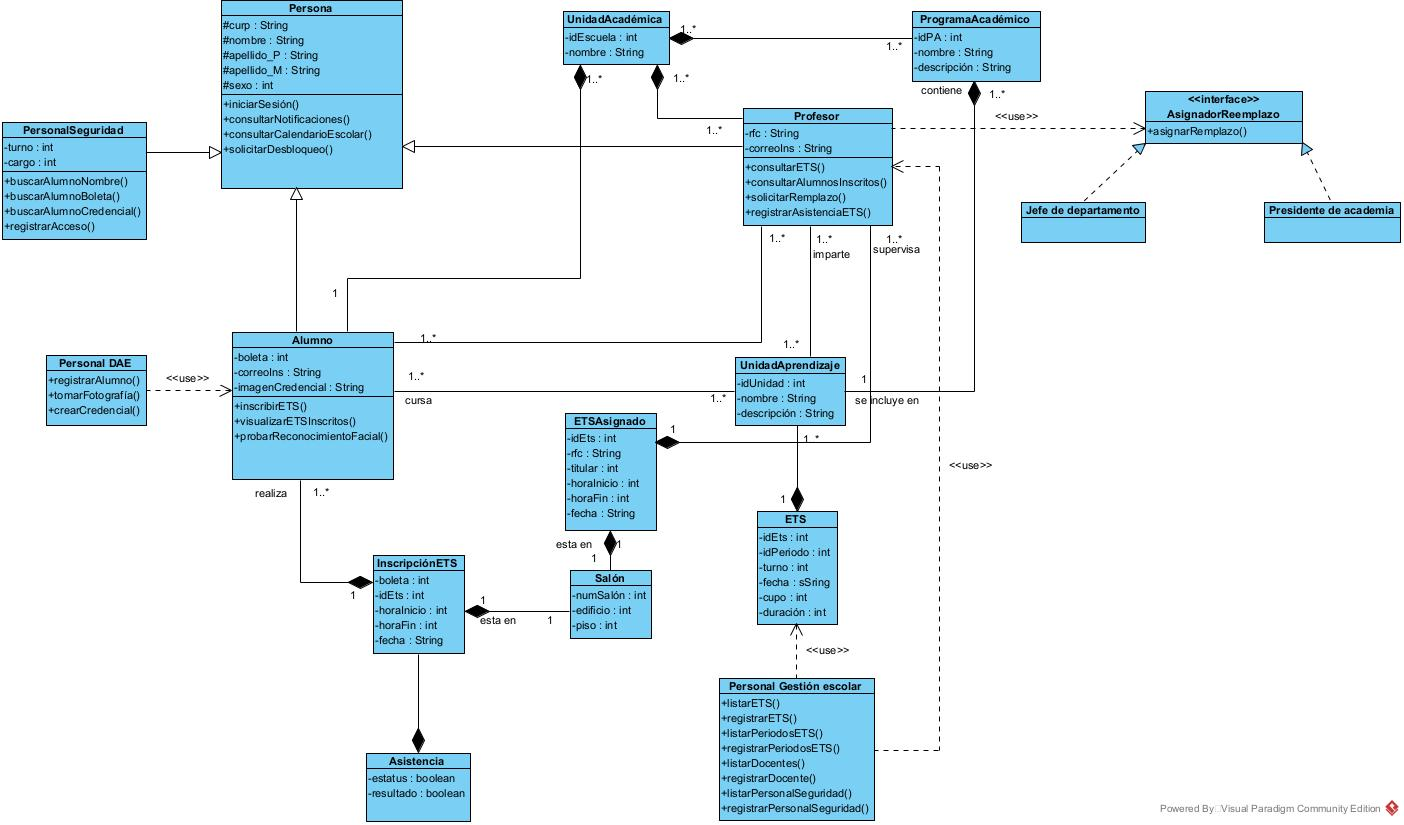
\includegraphics[width=.35\textwidth]{Clases/Clases}}
		\caption{Diagrama de clases.}
		\label{fig:Diagrama de clases}
	\end{center}
\end{figure}

\section{Diagramas de secuencia}

\begin{figure}[htbp!]
	\begin{center}
		\fbox{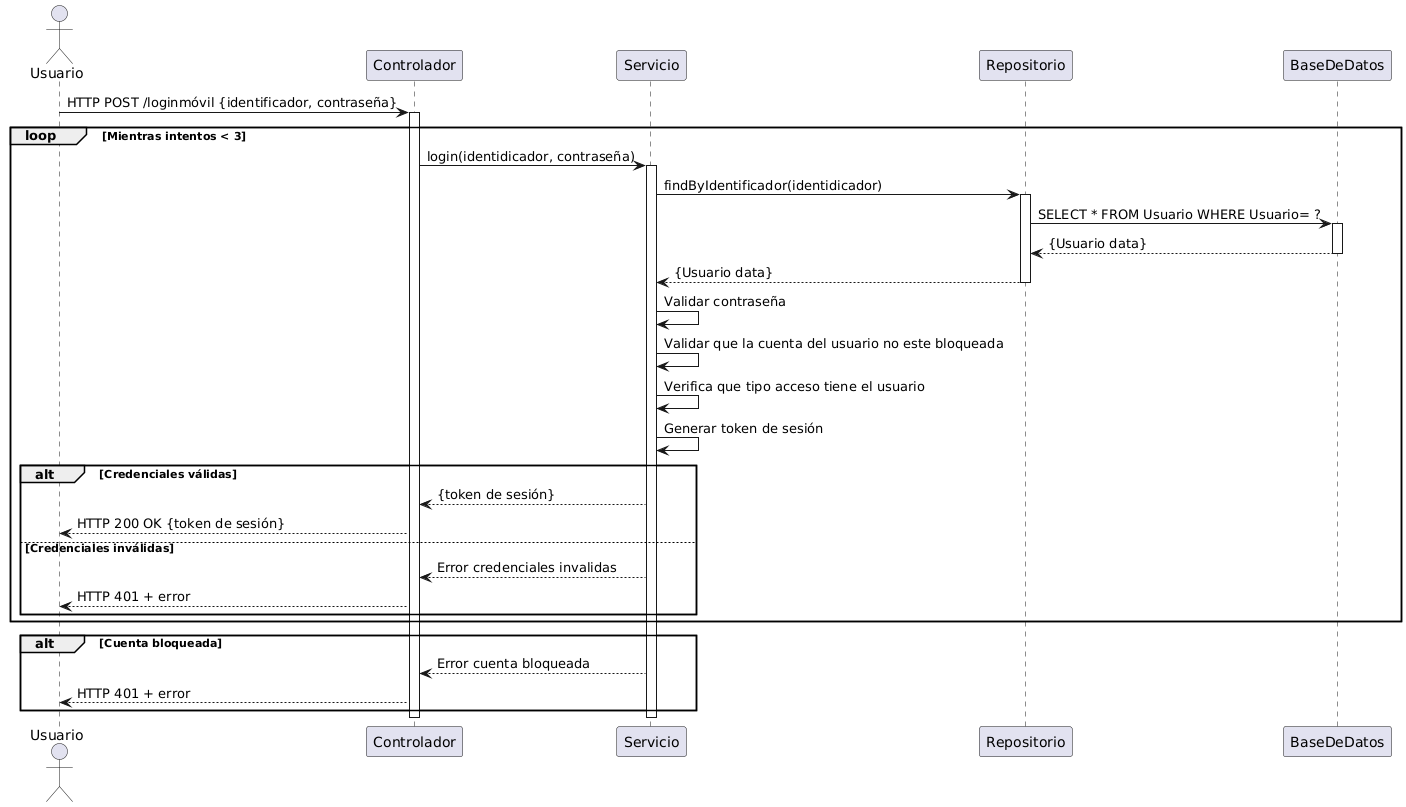
\includegraphics[width=.35\textwidth]{Secuencia/CU-01.png}}
		\caption{Diagrama de secuencia del caso de uso número 01 (Iniciar sesión del sistema móvil).}
		\label{fig:Diagrama de secuencia CU-01}
	\end{center}
\end{figure}

\begin{figure}[htbp!]
	\begin{center}
		\fbox{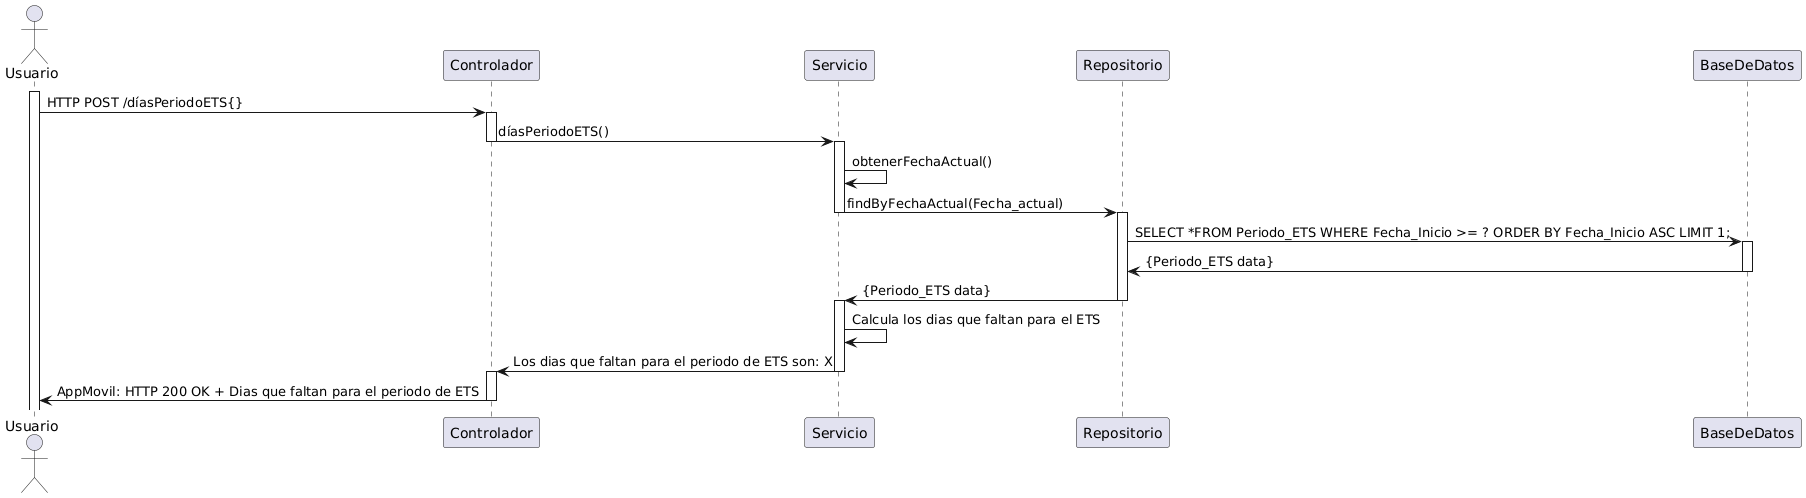
\includegraphics[width=.35\textwidth]{Secuencia/CU-02.png}}
		\caption{Diagrama de secuencia del caso de uso número 02 (Consultar calendario escolar).}
		\label{fig:Diagrama de secuencia CU-02}
	\end{center}
\end{figure}

\begin{figure}[htbp!]
	\begin{center}
		\fbox{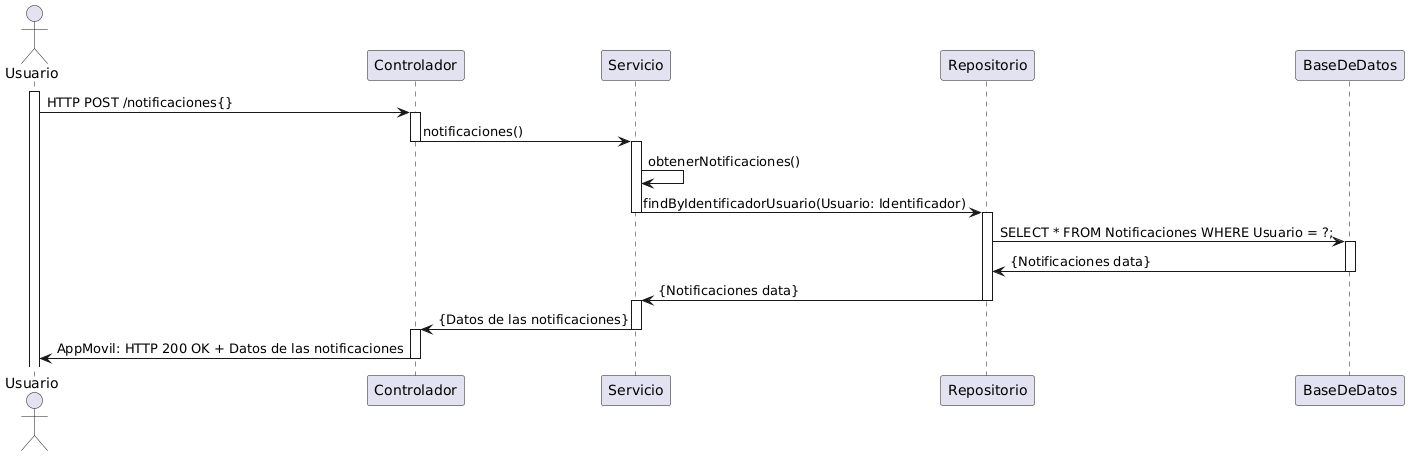
\includegraphics[width=.35\textwidth]{Secuencia/CU-03.png}}
		\caption{Diagrama de secuencia del caso de uso número 03 (Consultar notificaciones).}
		\label{fig:Diagrama se secuencia CU-03}
	\end{center}
\end{figure}

\begin{figure}[htbp!]
	\begin{center}
		\fbox{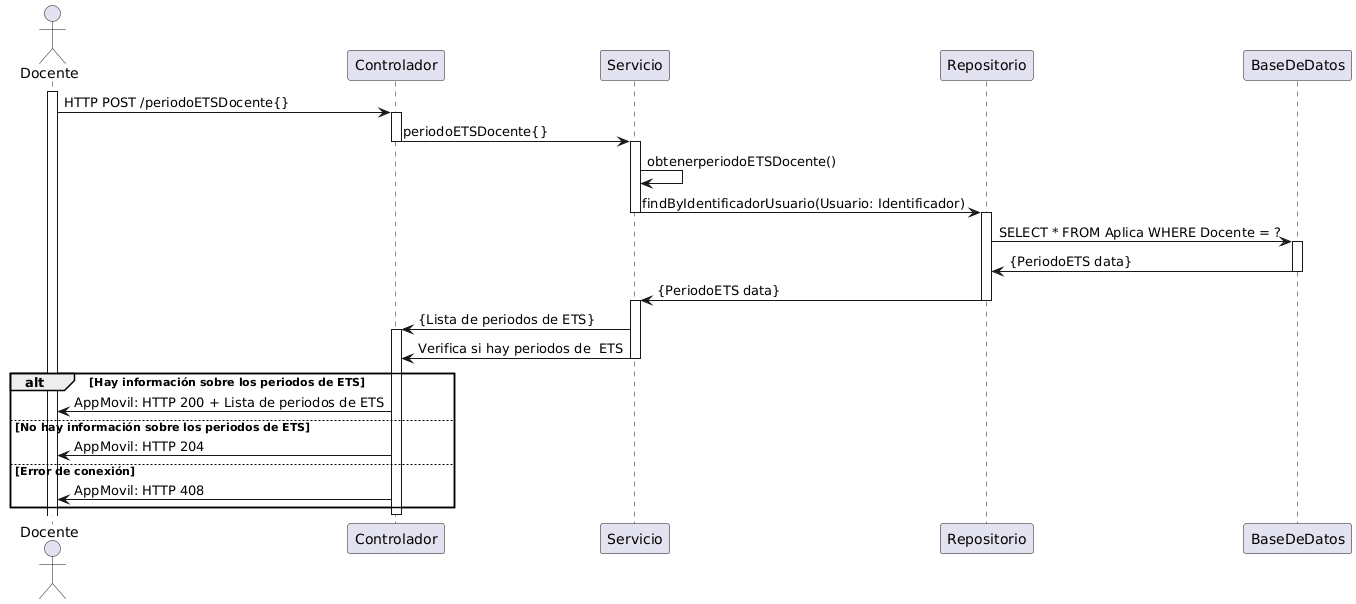
\includegraphics[width=.35\textwidth]{Secuencia/CU-04.png}}
		\caption{Diagrama de secuencia del caso de uso número 04 (Consultar periodos de ETS asignados al docente).}
		\label{fig:Diagrama de secuencia CU-04}
	\end{center}
\end{figure}

\begin{figure}[htbp!]
	\begin{center}
		\fbox{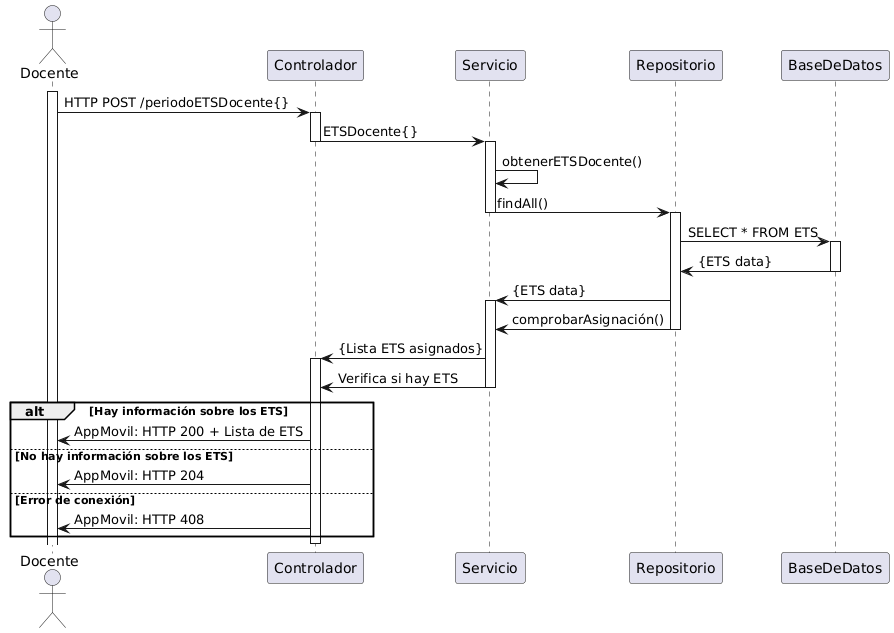
\includegraphics[width=.35\textwidth]{Secuencia/CU-05.png}}
		\caption{Diagrama de secuencia del caso de uso número 05 (Consultar ETS asignados).}
		\label{fig:Diagrama de secuencia CU-05}
	\end{center}
\end{figure}

\begin{figure}[htbp!]
	\begin{center}
		\fbox{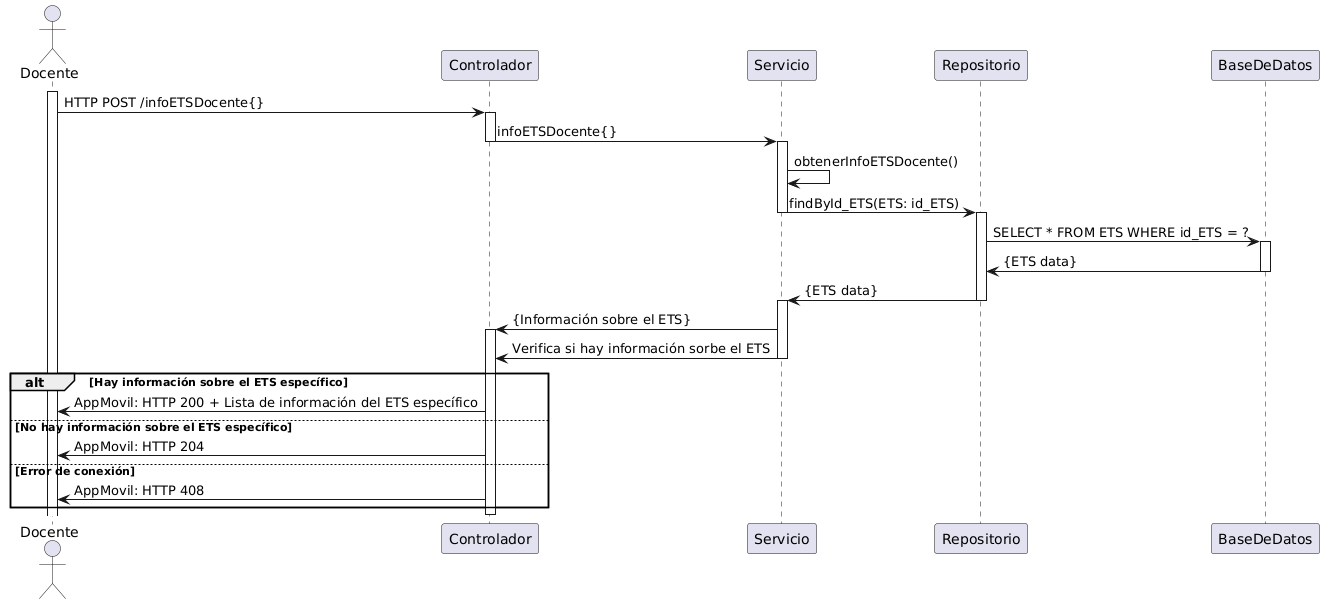
\includegraphics[width=.35\textwidth]{Secuencia/CU-06.png}}
		\caption{Diagrama de secuencia del caso de uso número 06 (CU-06).}
		\label{fig:Diagrama de secuencia CU-06}
	\end{center}
\end{figure}

\begin{figure}[htbp!]
	\begin{center}
		\fbox{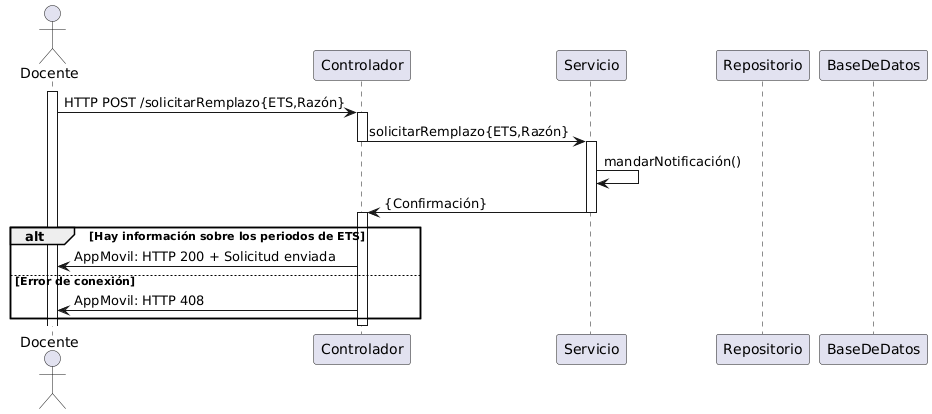
\includegraphics[width=.35\textwidth]{Secuencia/CU-07.png}}
		\caption{Diagrama de secuencia del caso de uso número 07 (CU-07).}
		\label{fig:Diagrama de secuencia CU-07}
	\end{center}
\end{figure}

\begin{figure}[htbp!]
	\begin{center}
		\fbox{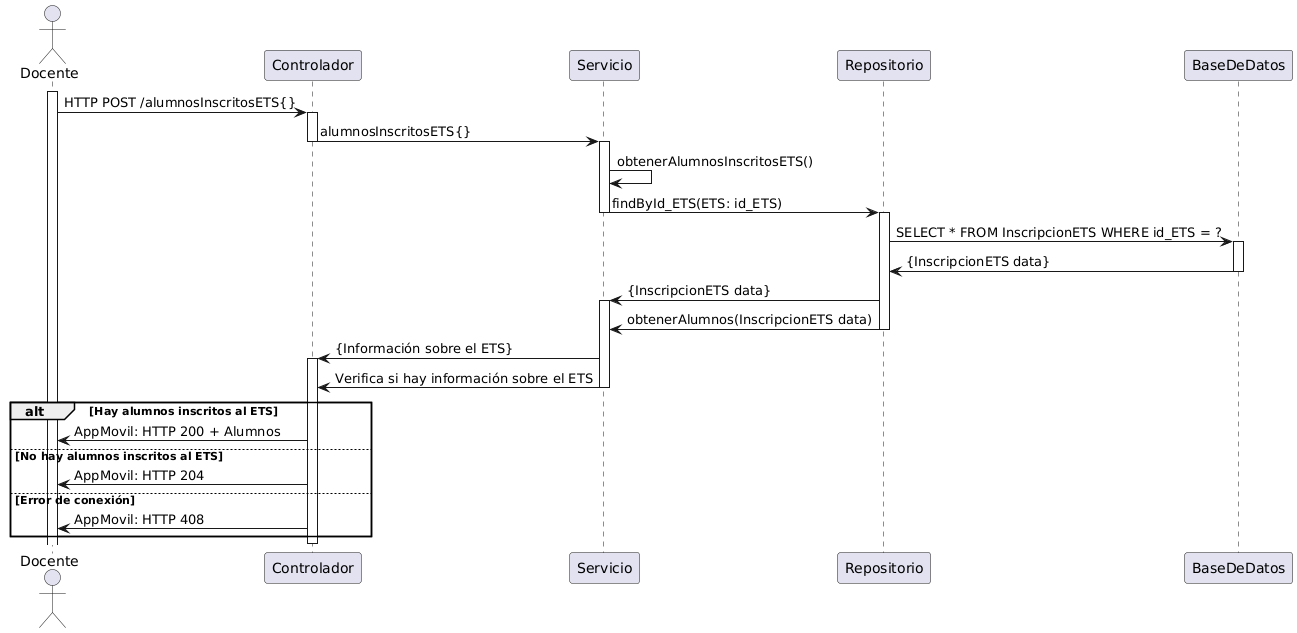
\includegraphics[width=.35\textwidth]{Secuencia/CU-08.png}}
		\caption{Diagrama de secuencia del caso de uso número 08 (CU-08).}
		\label{fig:Diagrama de secuencia CU-08}
	\end{center}
\end{figure}

\begin{figure}[htbp!]
	\begin{center}
		\fbox{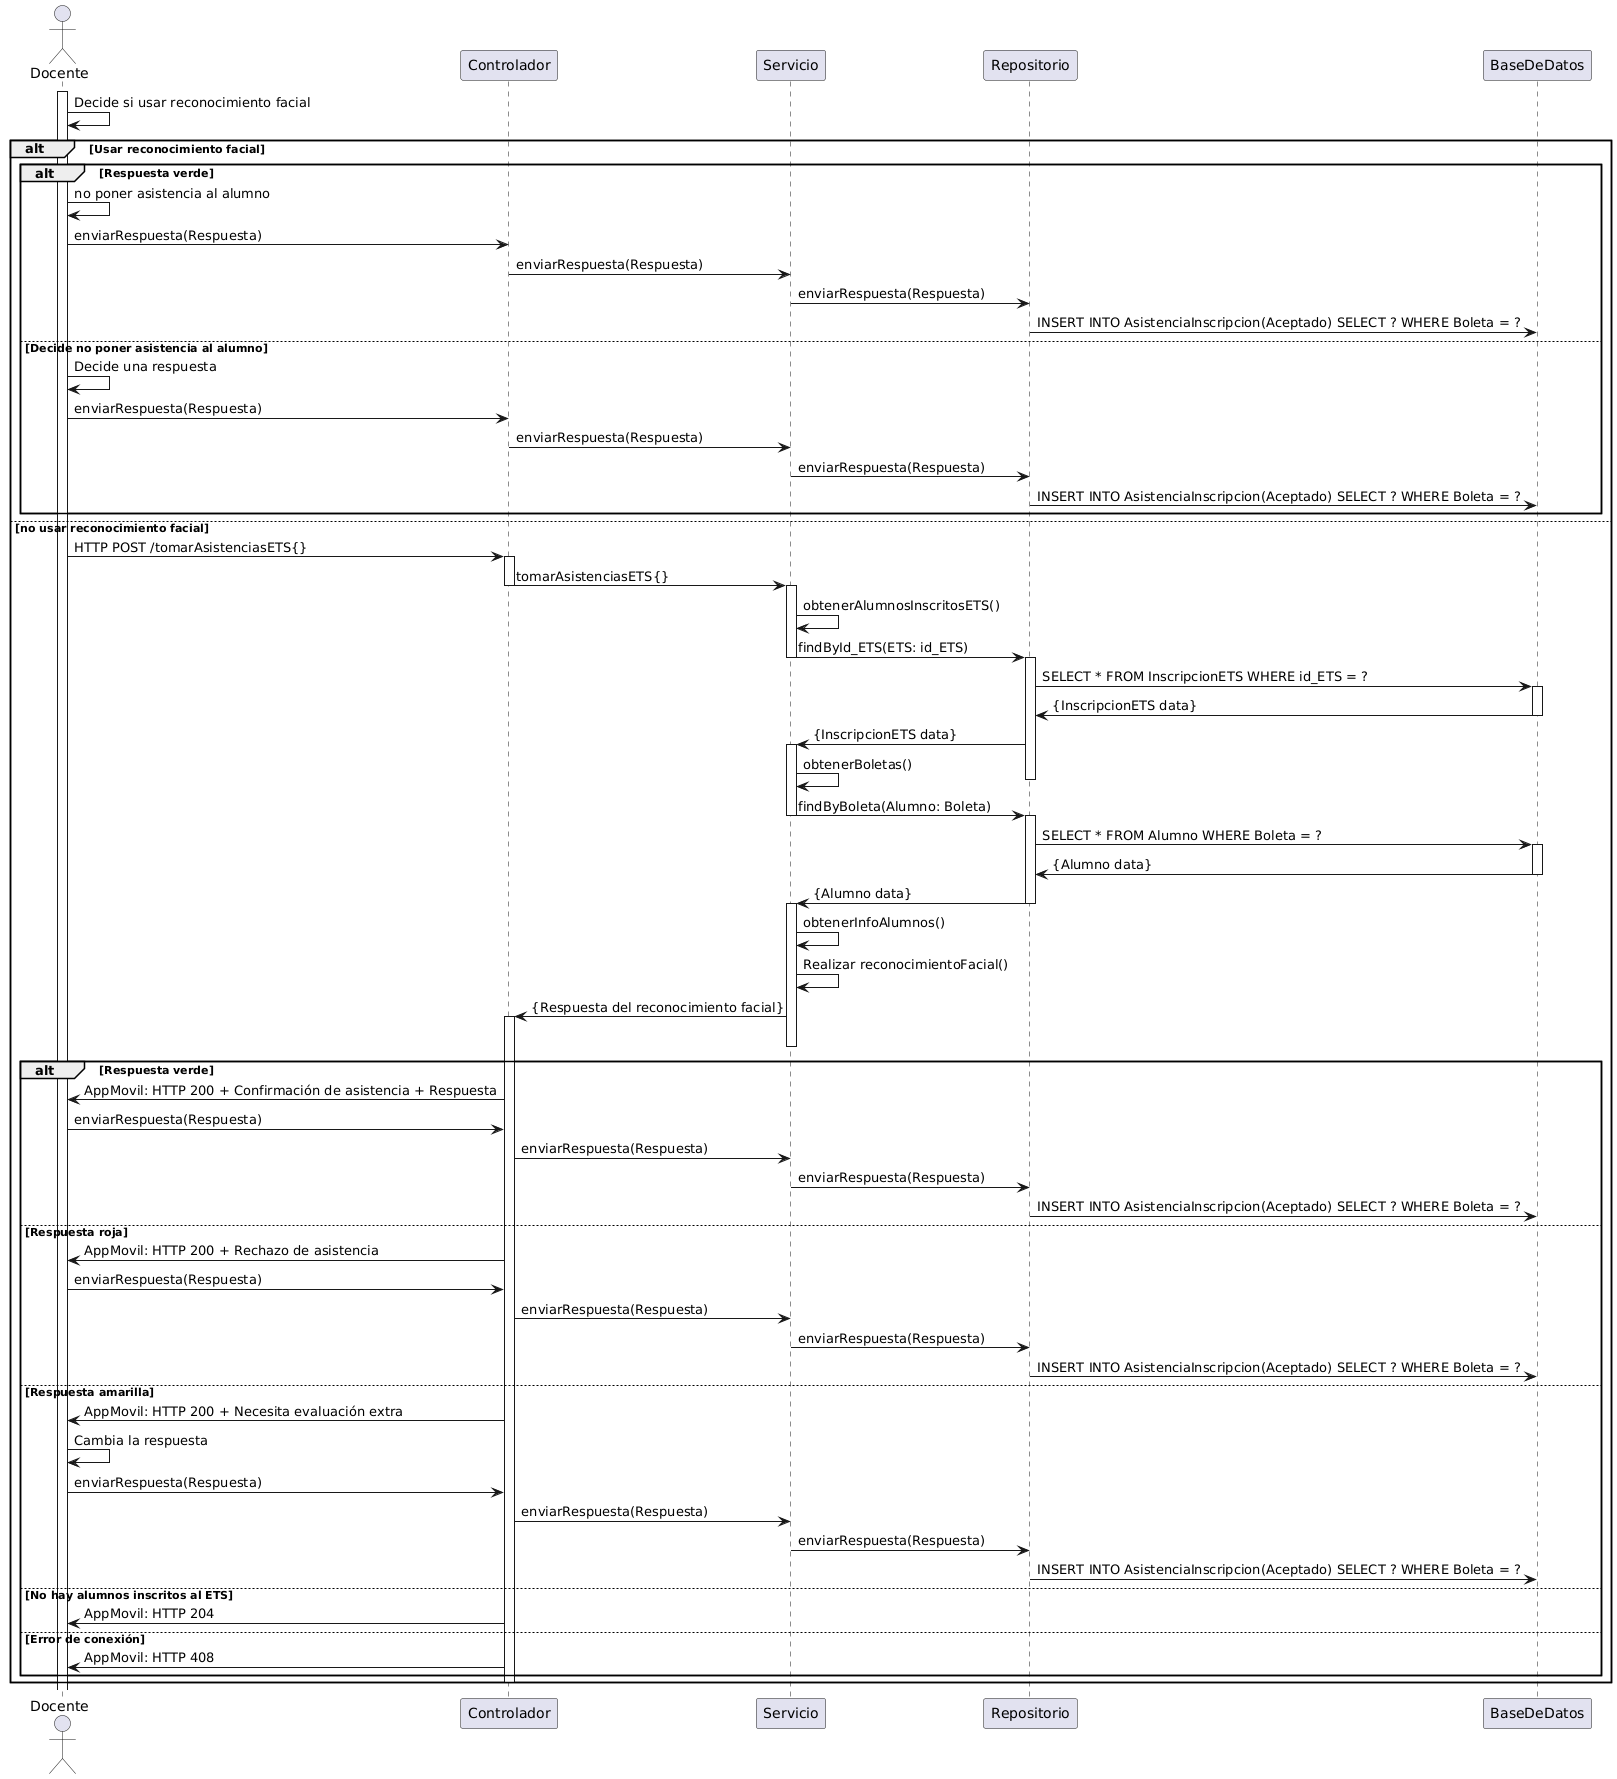
\includegraphics[width=.35\textwidth]{Secuencia/CU-09.png}}
		\caption{Diagrama de secuencia del caso de uso número 09 (CU-09).}
		\label{fig:Diagrama de secuencia CU-09}
	\end{center}
\end{figure}

\begin{figure}[htbp!]
	\begin{center}
		\fbox{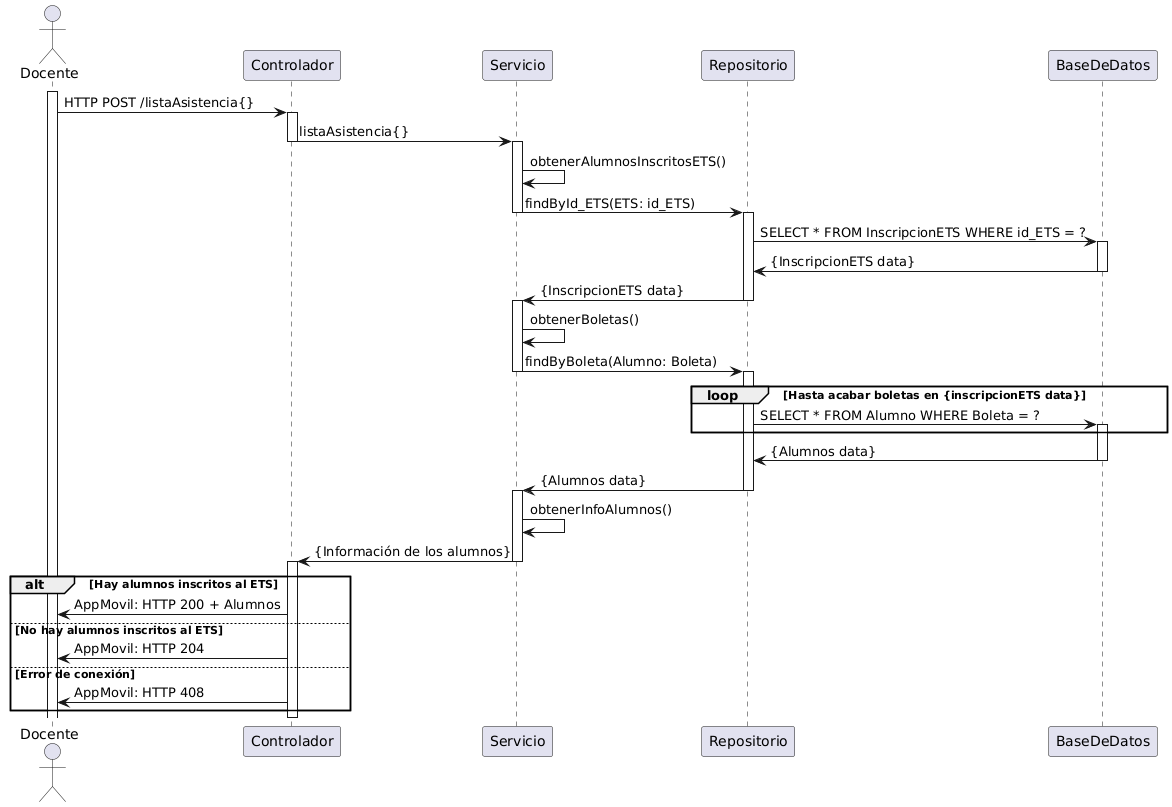
\includegraphics[width=.35\textwidth]{Secuencia/CU-10.png}}
		\caption{Diagrama de secuencia del caso de uso número 10 (CU-10).}
		\label{fig:Diagrama de secuencia CU-10}
	\end{center}
\end{figure}

\begin{figure}[htbp!]
	\begin{center}
		\fbox{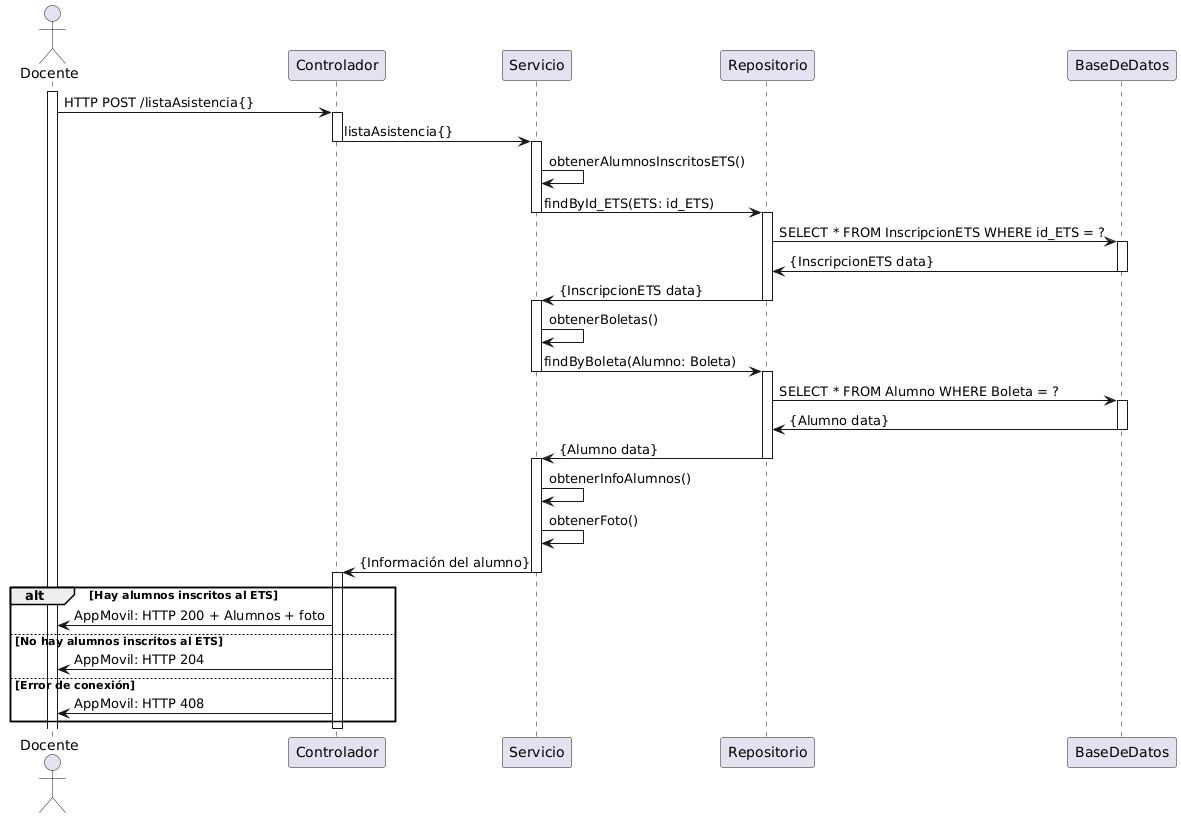
\includegraphics[width=.35\textwidth]{Secuencia/CU-11.png}}
		\caption{Diagrama de secuencia del caso de uso número 11 (CU-11).}
		\label{fig:Diagrama de secuencia CU-1}
	\end{center}
\end{figure}

\begin{figure}[htbp!]
	\begin{center}
		\fbox{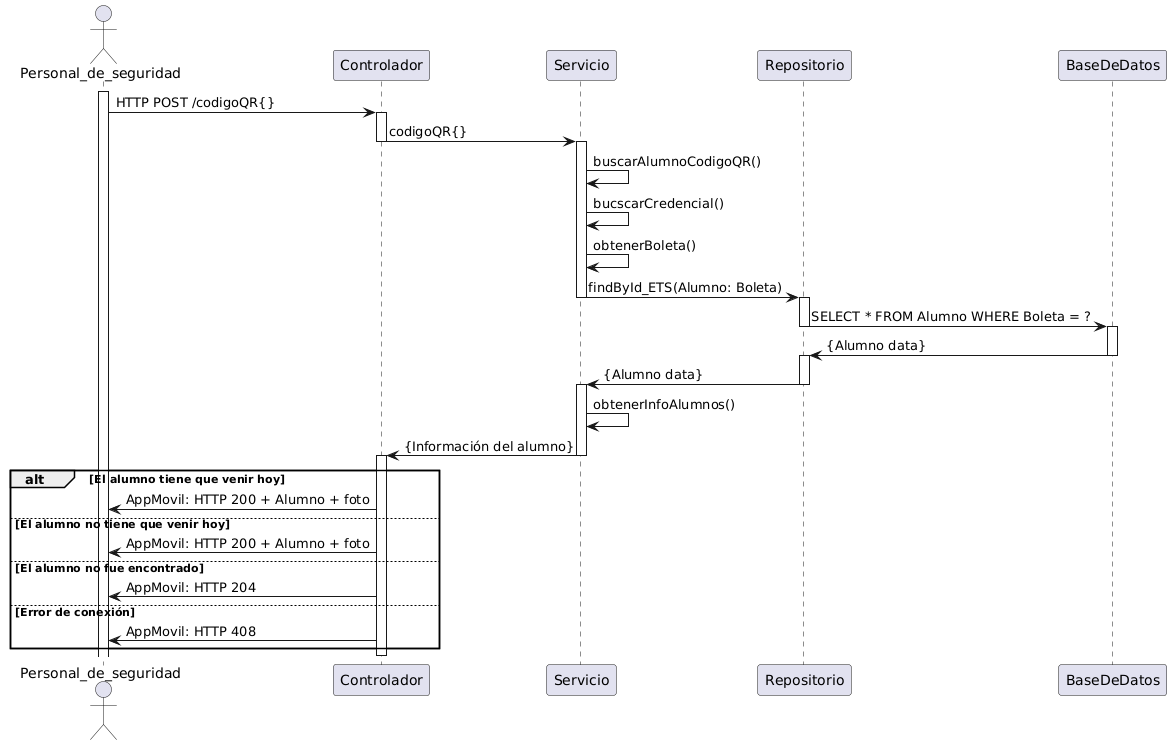
\includegraphics[width=.35\textwidth]{Secuencia/CU-12.png}}
		\caption{Diagrama de secuencia del caso de uso número 12 (CU-12).}
		\label{fig:Diagrama de secuencia CU-12}
	\end{center}
\end{figure}

\begin{figure}[htbp!]
	\begin{center}
		\fbox{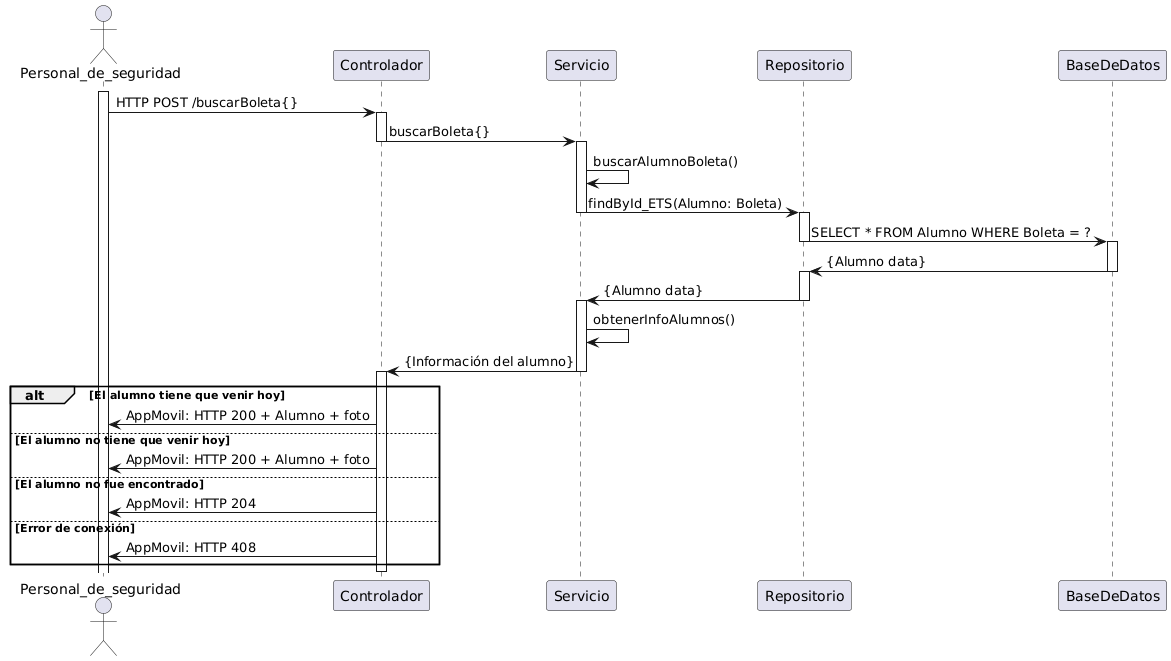
\includegraphics[width=.35\textwidth]{Secuencia/CU-13.png}}
		\caption{Diagrama de secuencia del caso de uso número 13 (CU-13).}
		\label{fig:Diagrama de secuencia CU-13}
	\end{center}
\end{figure}

\begin{figure}[htbp!]
	\begin{center}
		\fbox{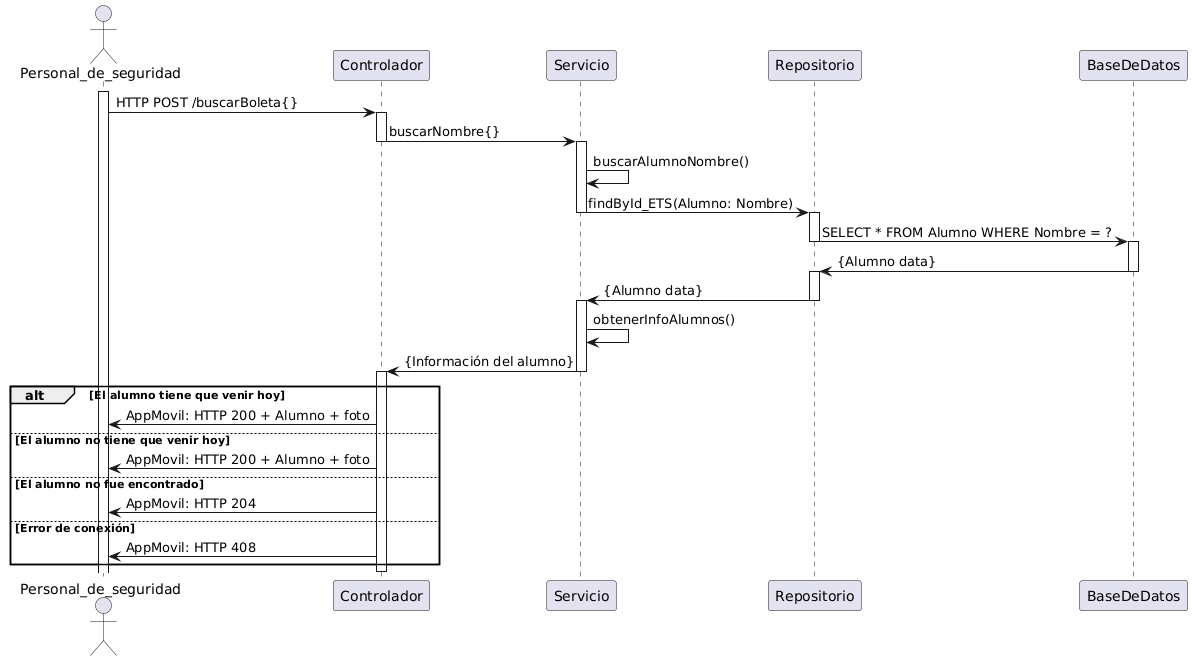
\includegraphics[width=.35\textwidth]{Secuencia/CU-14.png}}
		\caption{Diagrama de secuencia del caso de uso número 14 (CU-14).}
		\label{fig:Diagrama de secuencia CU-14}
	\end{center}
\end{figure}

\begin{figure}[htbp!]
	\begin{center}
		\fbox{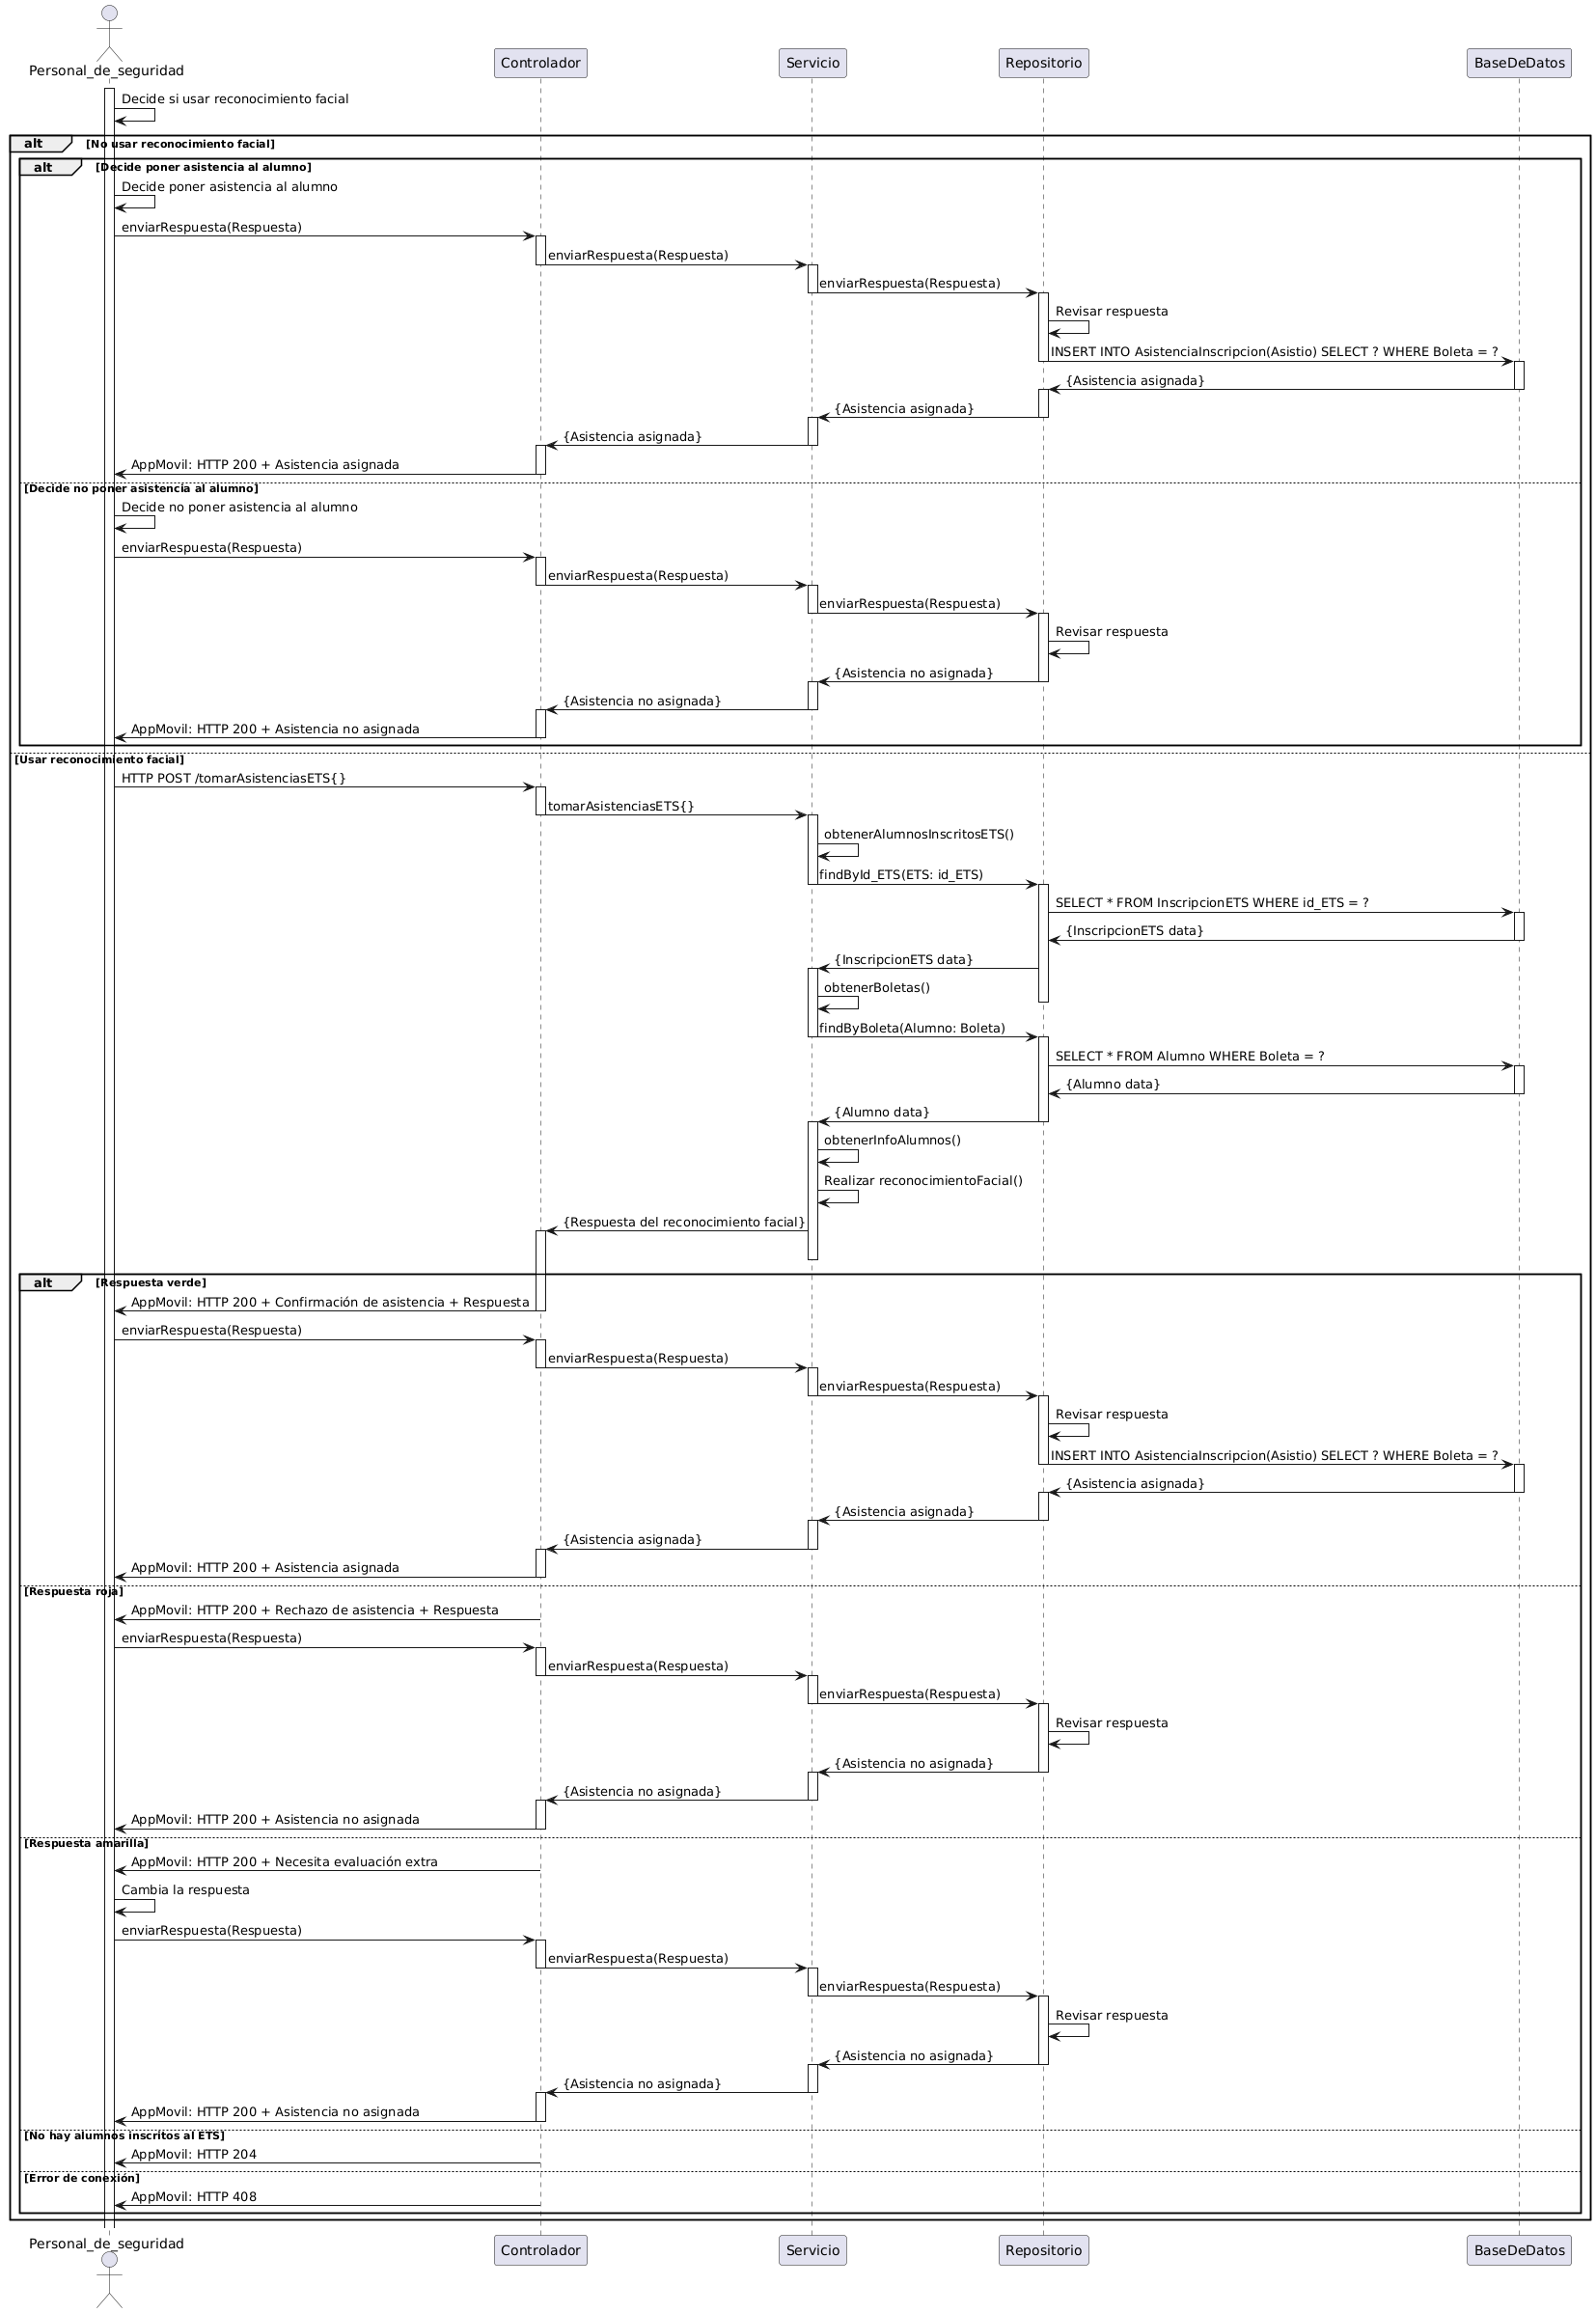
\includegraphics[width=.35\textwidth]{Secuencia/CU-15.png}}
		\caption{Diagrama de secuencia del caso de uso número 15 (CU-15).}
		\label{fig:Diagrama de secuencia CU-15}
	\end{center}
\end{figure}

\begin{figure}[htbp!]
	\begin{center}
		\fbox{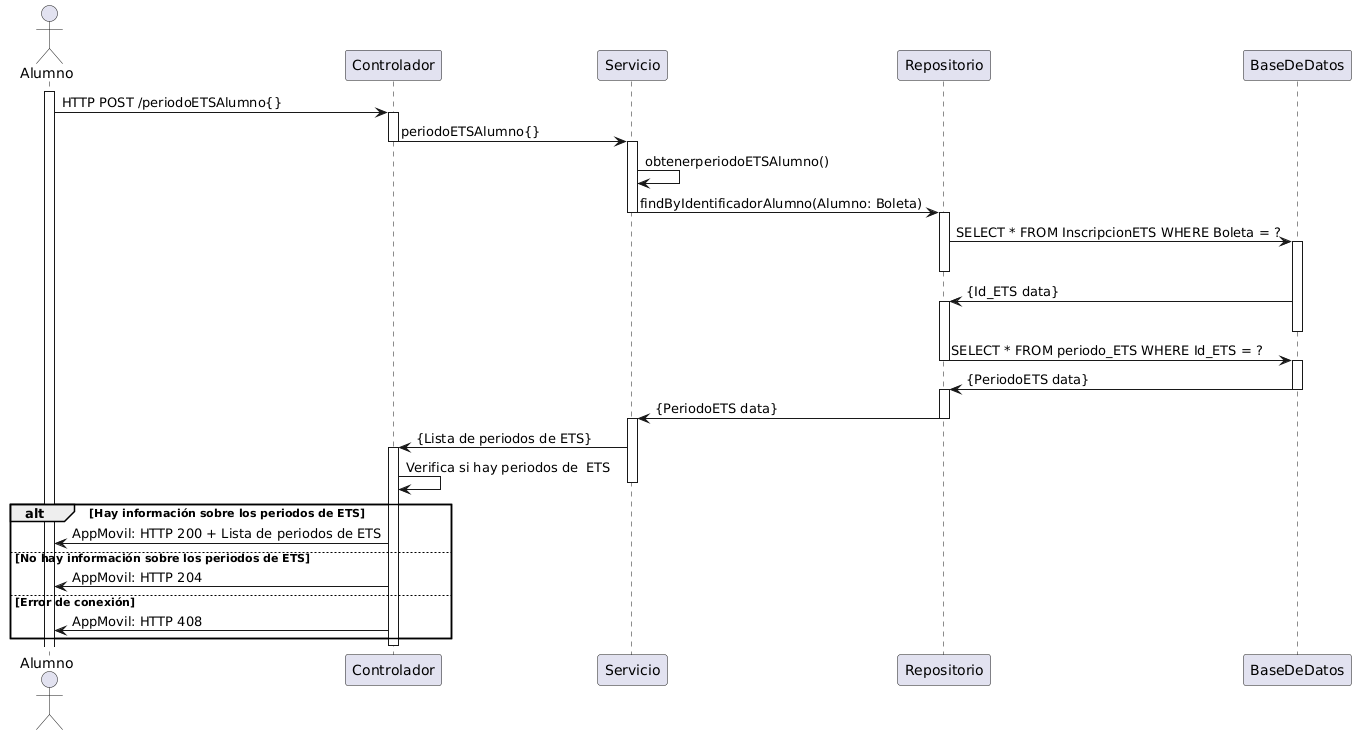
\includegraphics[width=.35\textwidth]{Secuencia/CU-16.png}}
		\caption{Diagrama de secuencia del caso de uso número 16 (CU-16).}
		\label{fig:Diagrama de secuencia CU-16}
	\end{center}
\end{figure}

\begin{figure}[htbp!]
	\begin{center}
		\fbox{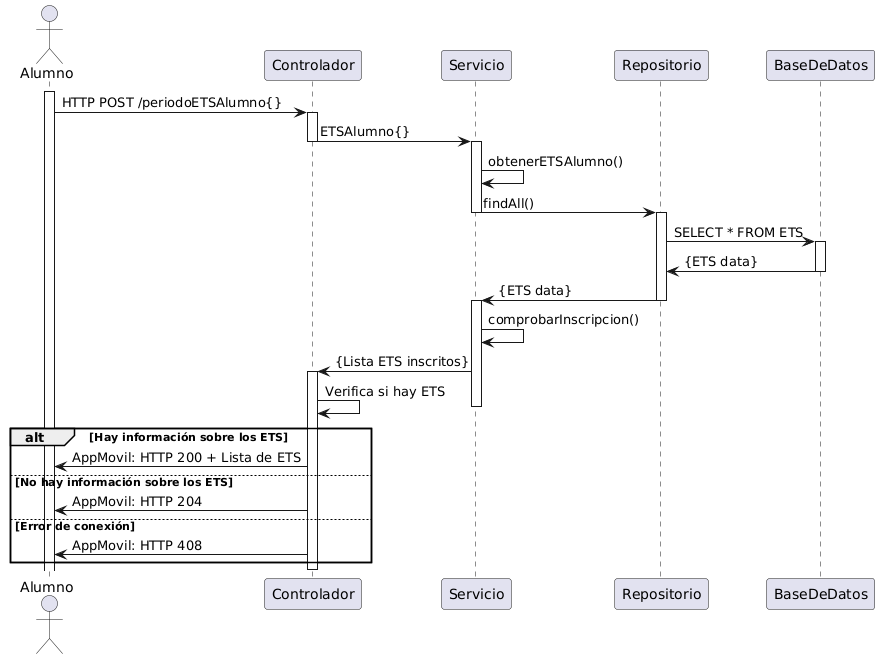
\includegraphics[width=.35\textwidth]{Secuencia/CU-17.png}}
		\caption{Diagrama de secuencia del caso de uso número 04 (CU-17).}
		\label{fig:Diagrama de secuencia CU-17}
	\end{center}
\end{figure}

\begin{figure}[htbp!]
	\begin{center}
		\fbox{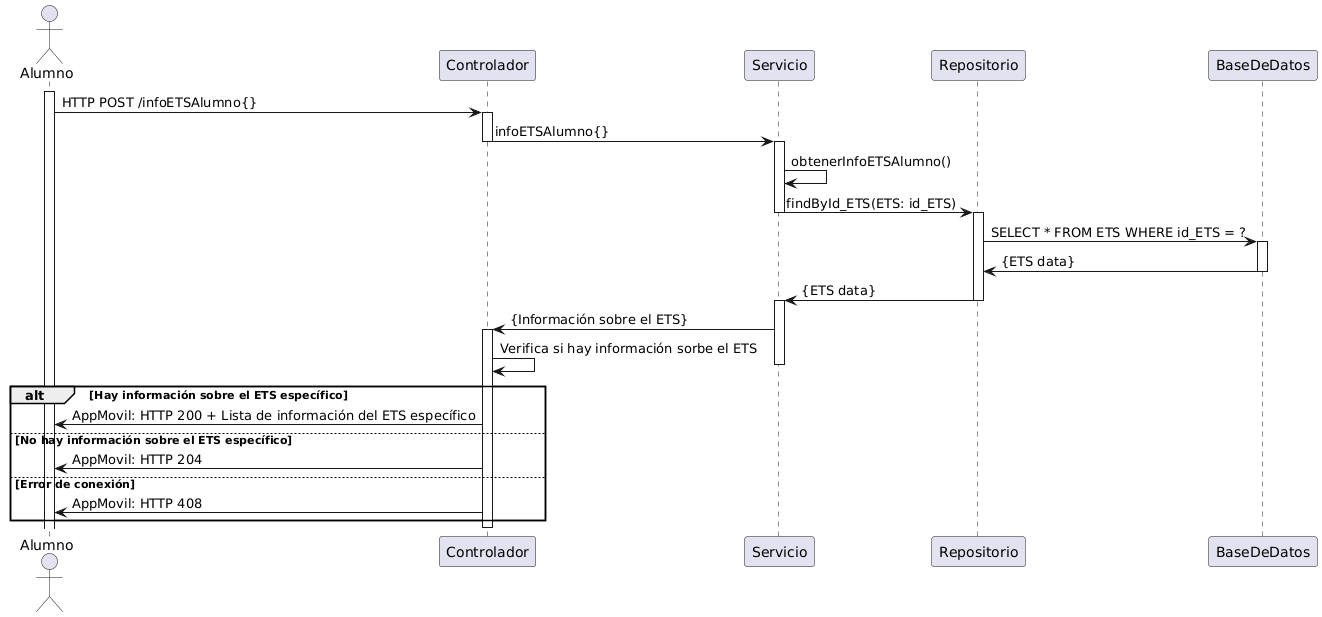
\includegraphics[width=.35\textwidth]{Secuencia/CU-18.png}}
		\caption{Diagrama de secuencia del caso de uso número 18 (CU-18).}
		\label{fig:Diagrama de secuencia CU-18}
	\end{center}
\end{figure}

\begin{figure}[htbp!]
	\begin{center}
		\fbox{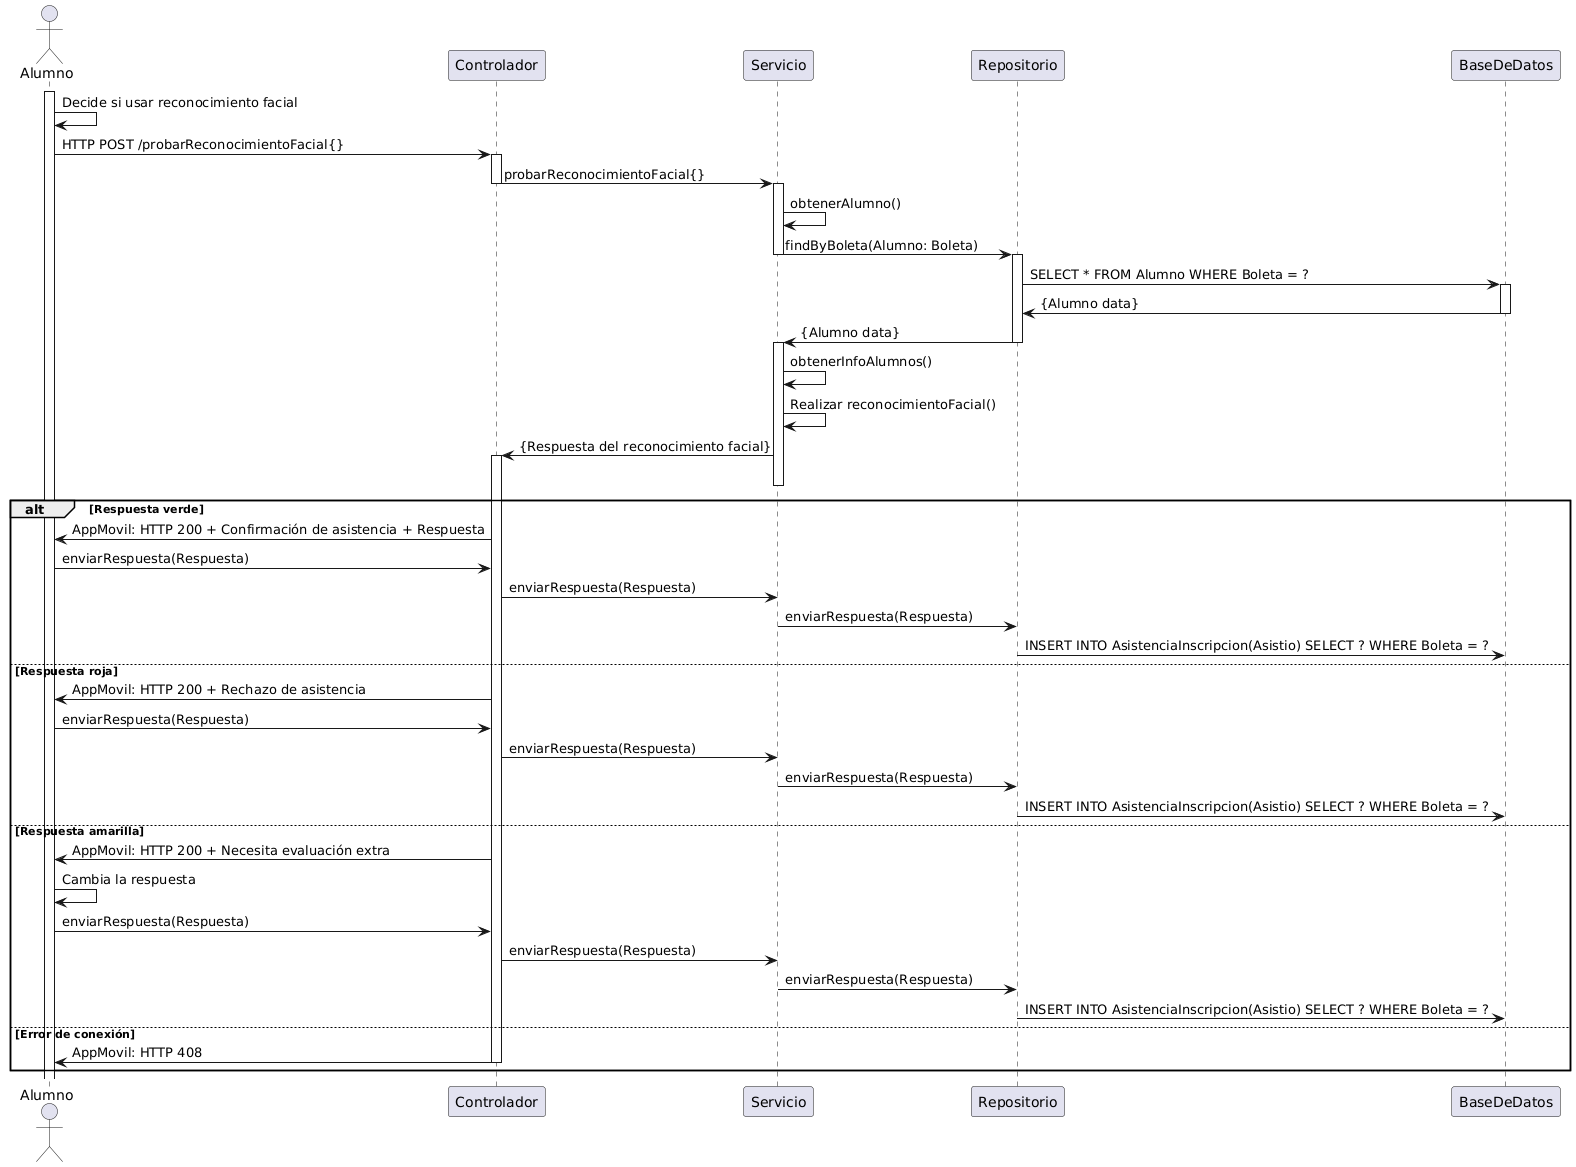
\includegraphics[width=.35\textwidth]{Secuencia/CU-19.png}}
		\caption{Diagrama de secuencia del caso de uso número 19 (CU-19).}
		\label{fig:Diagrama de secuencia CU-19}
	\end{center}
\end{figure}

\begin{figure}[htbp!]
	\begin{center}
		\fbox{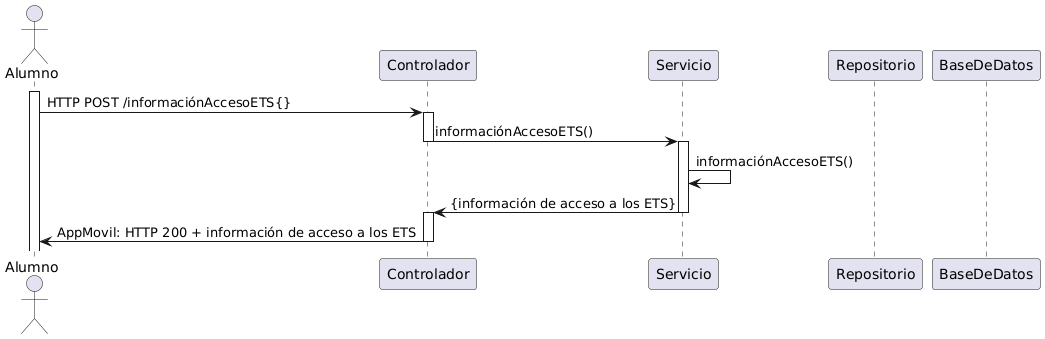
\includegraphics[width=.35\textwidth]{Secuencia/CU-20.png}}
		\caption{Diagrama de secuencia del caso de uso número 20 (CU-20).}
		\label{fig:Diagrama de secuencia CU-20}
	\end{center}
\end{figure}

\begin{figure}[htbp!]
	\begin{center}
		\fbox{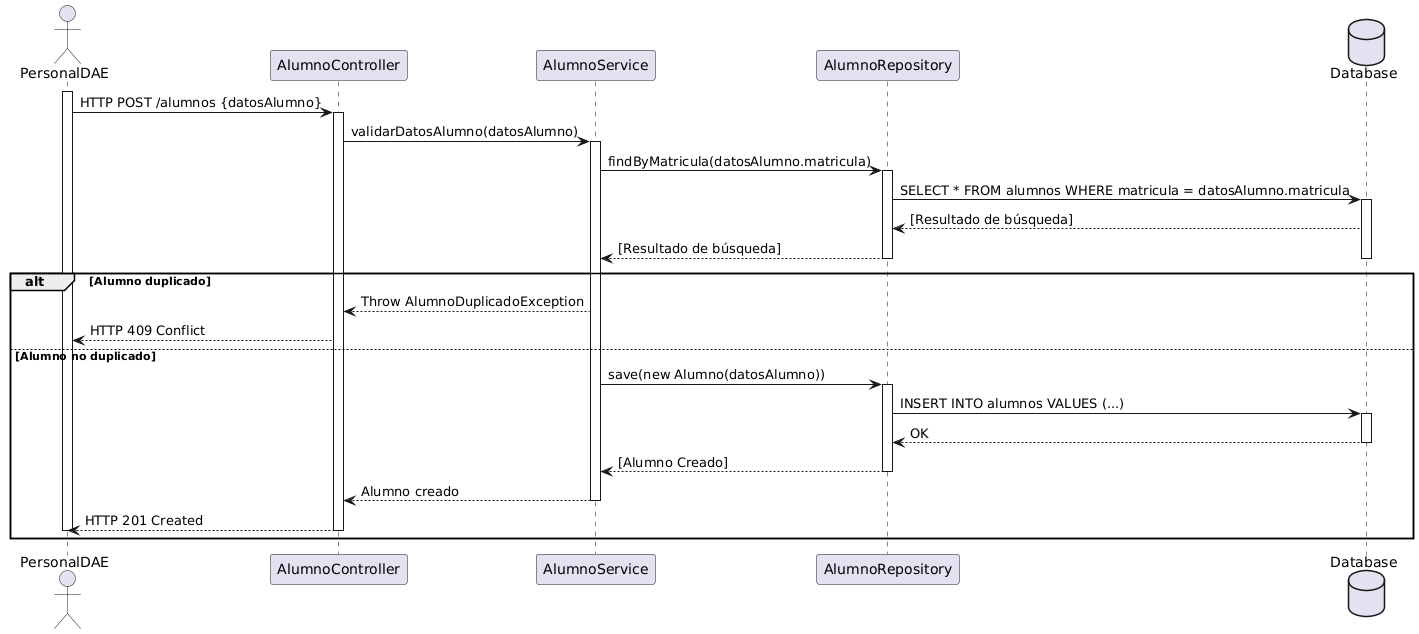
\includegraphics[width=.35\textwidth]{Secuencia/CU-21.png}}
		\caption{Diagrama de secuencia del caso de uso número 21 (CU-21).}
		\label{fig:Diagrama de secuencia CU-21}
	\end{center}
\end{figure}

\begin{figure}[htbp!]
	\begin{center}
		\fbox{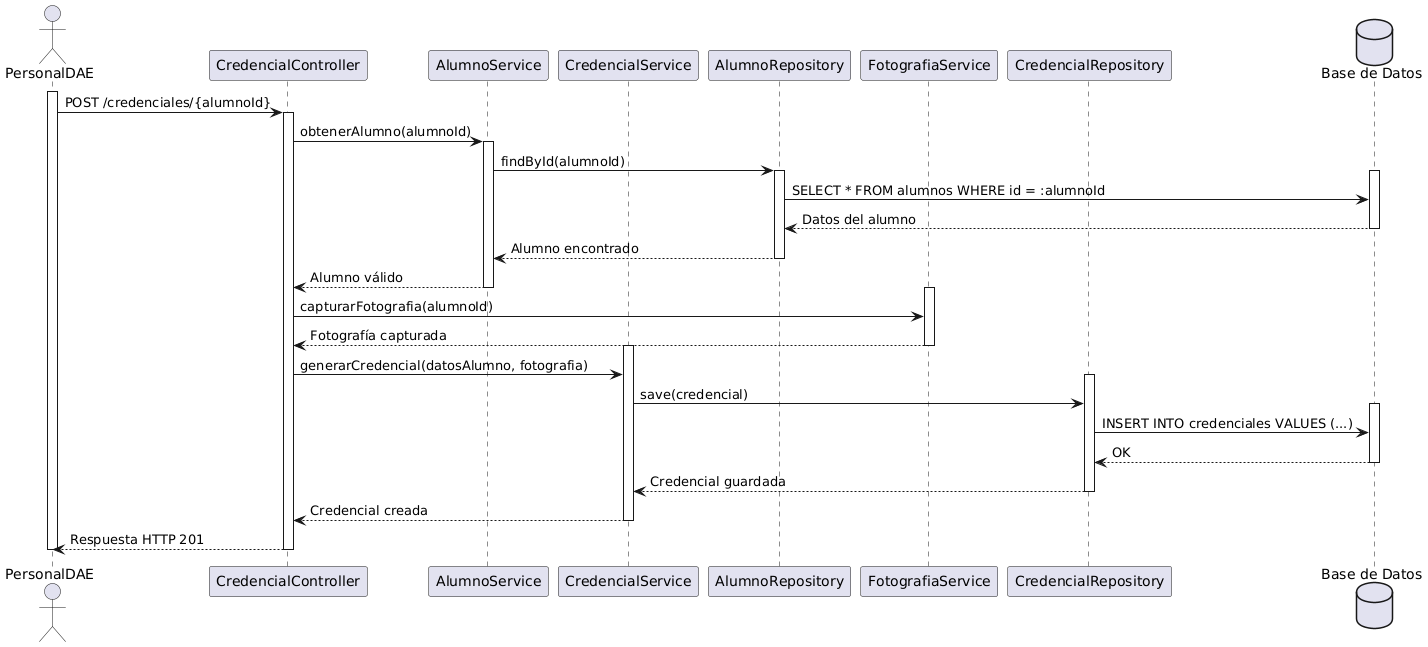
\includegraphics[width=.35\textwidth]{Secuencia/CU-22_23.png}}
		\caption{Diagrama de secuencia del caso de uso número 22 y 23 (CU-22 y CU23).}
		\label{fig:Diagrama de secuencia CU-22 y CU23}
	\end{center}
\end{figure}

\begin{figure}[htbp!]
	\begin{center}
		\fbox{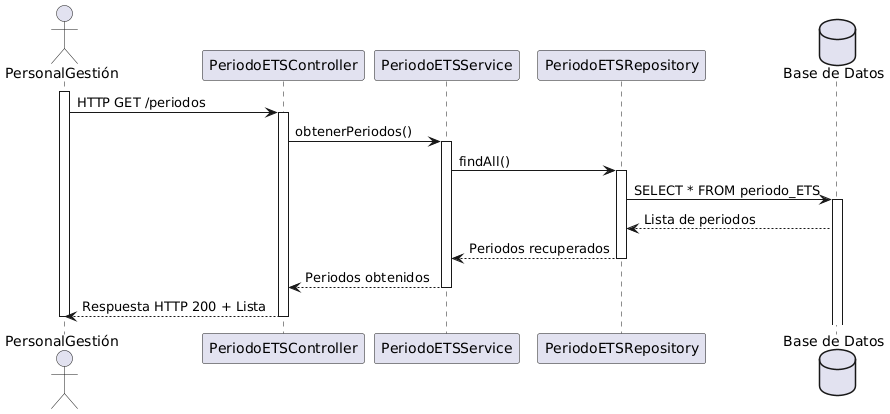
\includegraphics[width=.35\textwidth]{Secuencia/CU-24.png}}
		\caption{Diagrama de secuencia del caso de uso número 24 (CU-24).}
		\label{fig:Diagrama de secuencia CU-24}
	\end{center}
\end{figure}

\begin{figure}[htbp!]
	\begin{center}
		\fbox{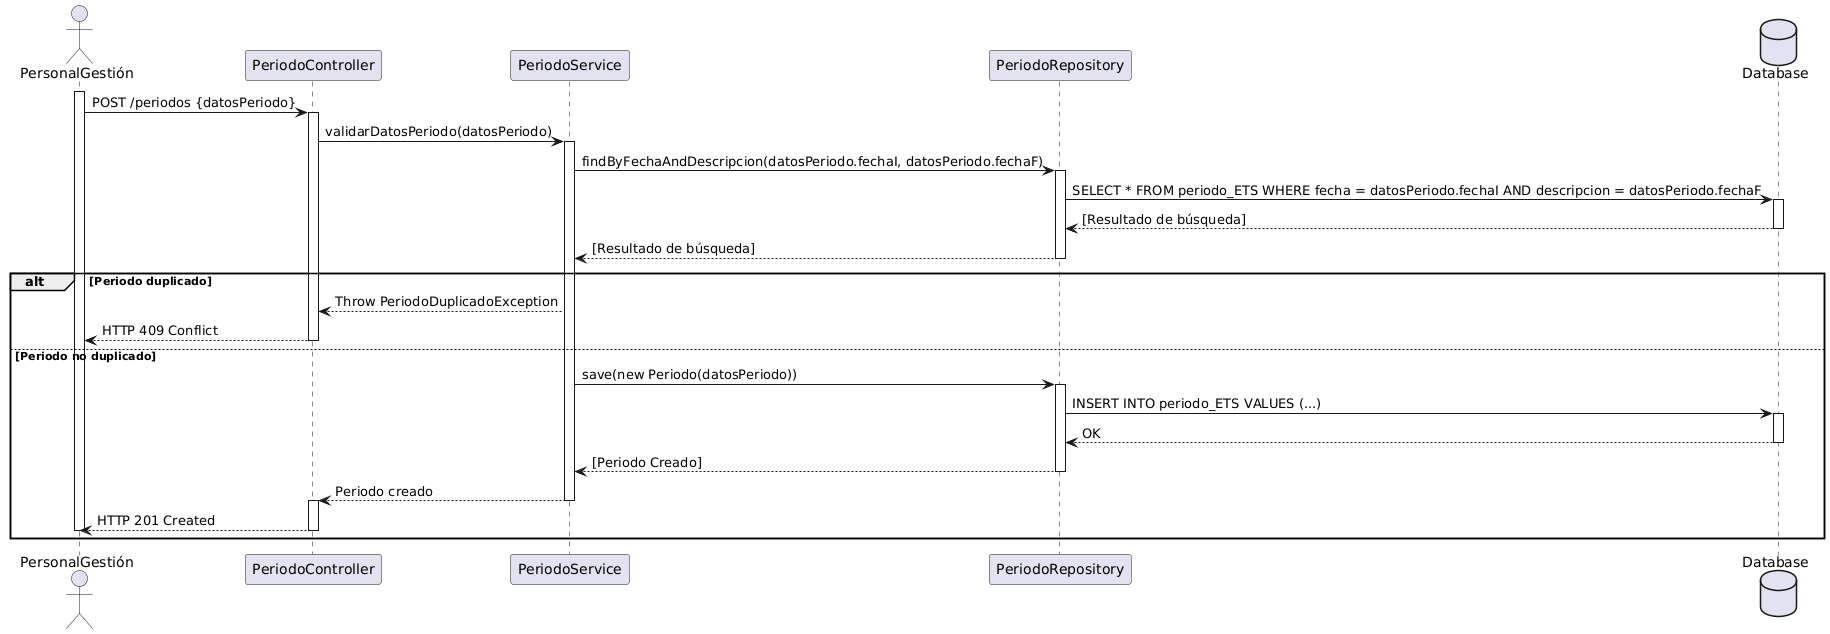
\includegraphics[width=.35\textwidth]{Secuencia/CU-25.png}}
		\caption{Diagrama de secuencia del caso de uso número 25 (CU-25).}
		\label{fig:Diagrama de secuencia CU-24}
	\end{center}
\end{figure}

\begin{figure}[htbp!]
	\begin{center}
		\fbox{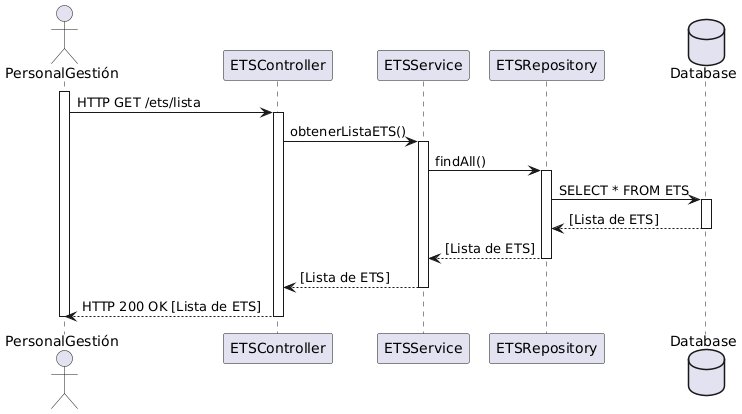
\includegraphics[width=.35\textwidth]{Secuencia/CU-28.png}}
		\caption{Diagrama de secuencia del caso de uso número 28 (CU-28).}
		\label{fig:Diagrama de secuencia CU-28}
	\end{center}
\end{figure}

\begin{figure}[htbp!]
	\begin{center}
		\fbox{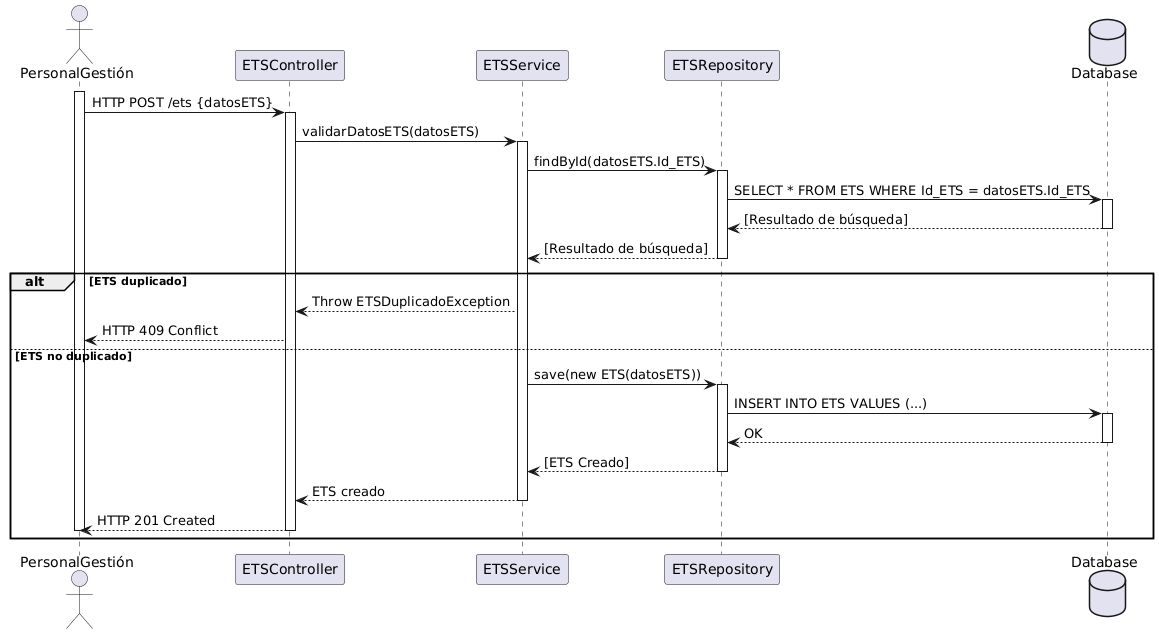
\includegraphics[width=.35\textwidth]{Secuencia/CU-29.png}}
		\caption{Diagrama de secuencia del caso de uso número 29 (CU-29).}
		\label{fig:Diagrama de secuencia CU-29}
	\end{center}
\end{figure}

\begin{figure}[htbp!]
	\begin{center}
		\fbox{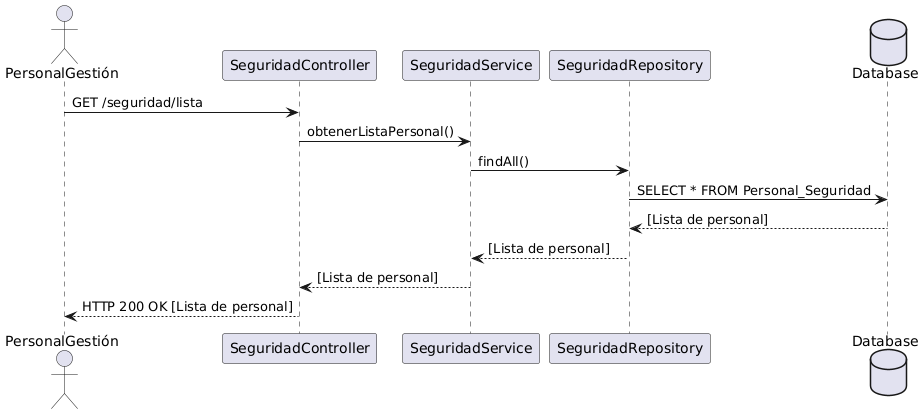
\includegraphics[width=.35\textwidth]{Secuencia/CU-32.png}}
		\caption{Diagrama de secuencia del caso de uso número 32 (CU-32).}
		\label{fig:Diagrama de secuencia CU-32}
	\end{center}
\end{figure}

\begin{figure}[htbp!]
	\begin{center}
		\fbox{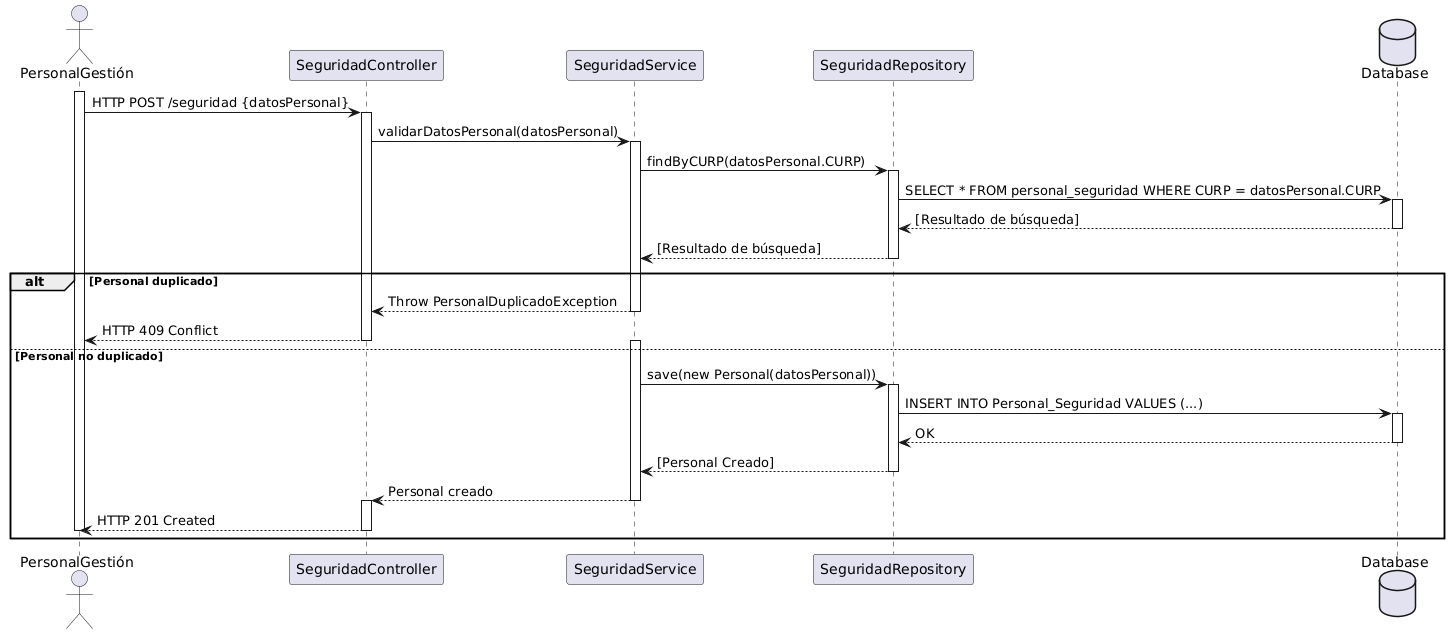
\includegraphics[width=.35\textwidth]{Secuencia/CU-33.png}}
		\caption{Diagrama de secuencia del caso de uso número 33 (CU-33).}
		\label{fig:Diagrama de secuencia CU-33}
	\end{center}
\end{figure}

\begin{figure}[htbp!]
	\begin{center}
		\fbox{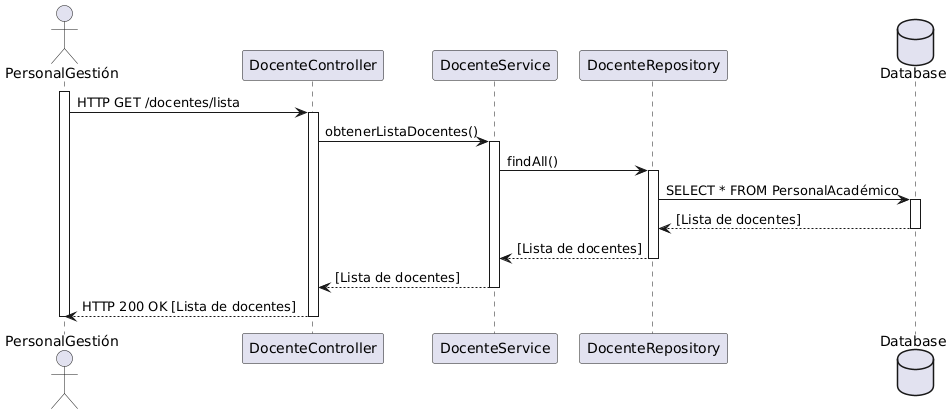
\includegraphics[width=.35\textwidth]{Secuencia/CU-36.png}}
		\caption{Diagrama de secuencia del caso de uso número 36 (CU-36).}
		\label{fig:Diagrama de secuencia CU-36}
	\end{center}
\end{figure}

\begin{figure}[htbp!]
	\begin{center}
		\fbox{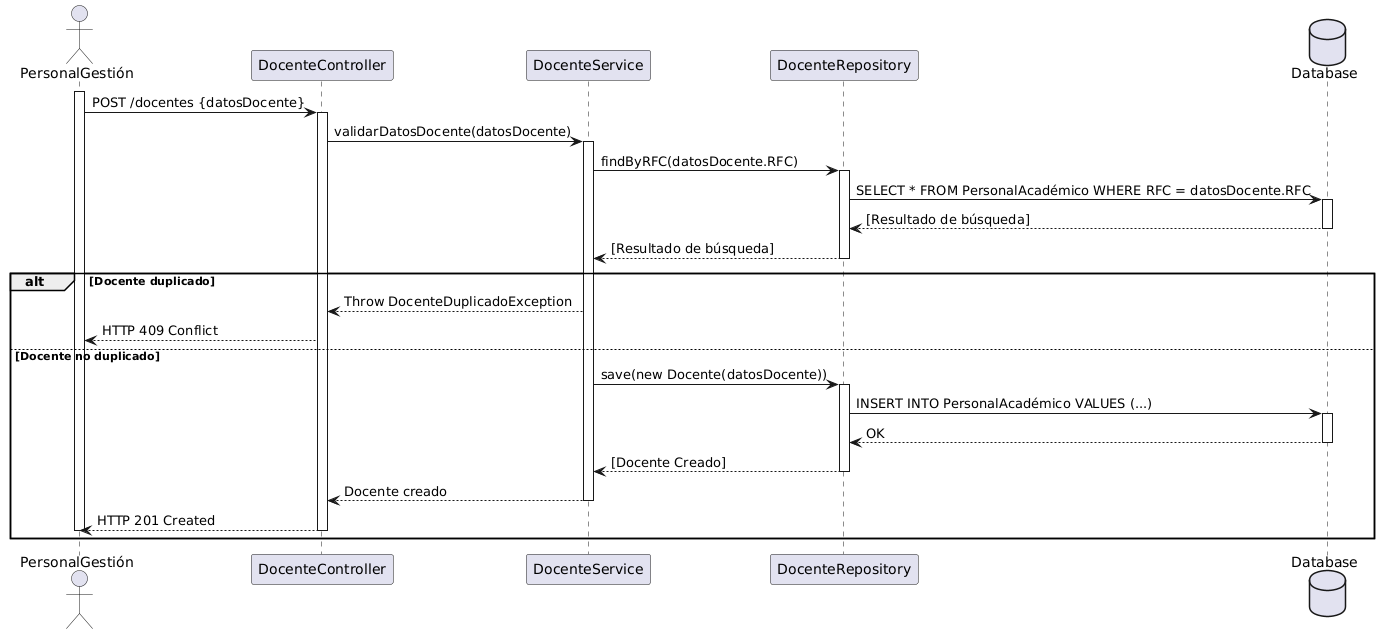
\includegraphics[width=.35\textwidth]{Secuencia/CU-37.png}}
		\caption{Diagrama de secuencia del caso de uso número 37 (CU-37).}
		\label{fig:Diagrama de secuencia CU-37}
	\end{center}
\end{figure}

\begin{figure}[htbp!]
	\begin{center}
		\fbox{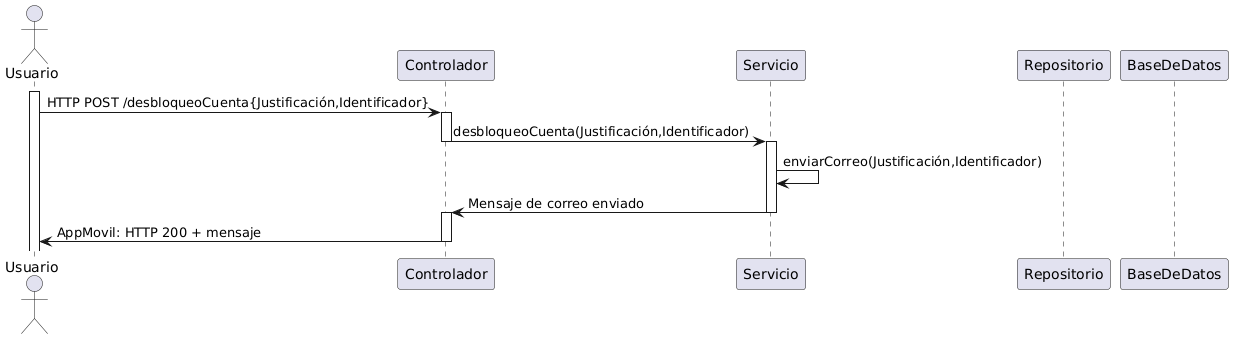
\includegraphics[width=.35\textwidth]{Secuencia/CU-40.png}}
		\caption{Diagrama de secuencia del caso de uso número 40 (CU-40).}
		\label{fig:Diagrama de secuencia CU-40}
	\end{center}
\end{figure}

\begin{figure}[htbp!]
	\begin{center}
		\fbox{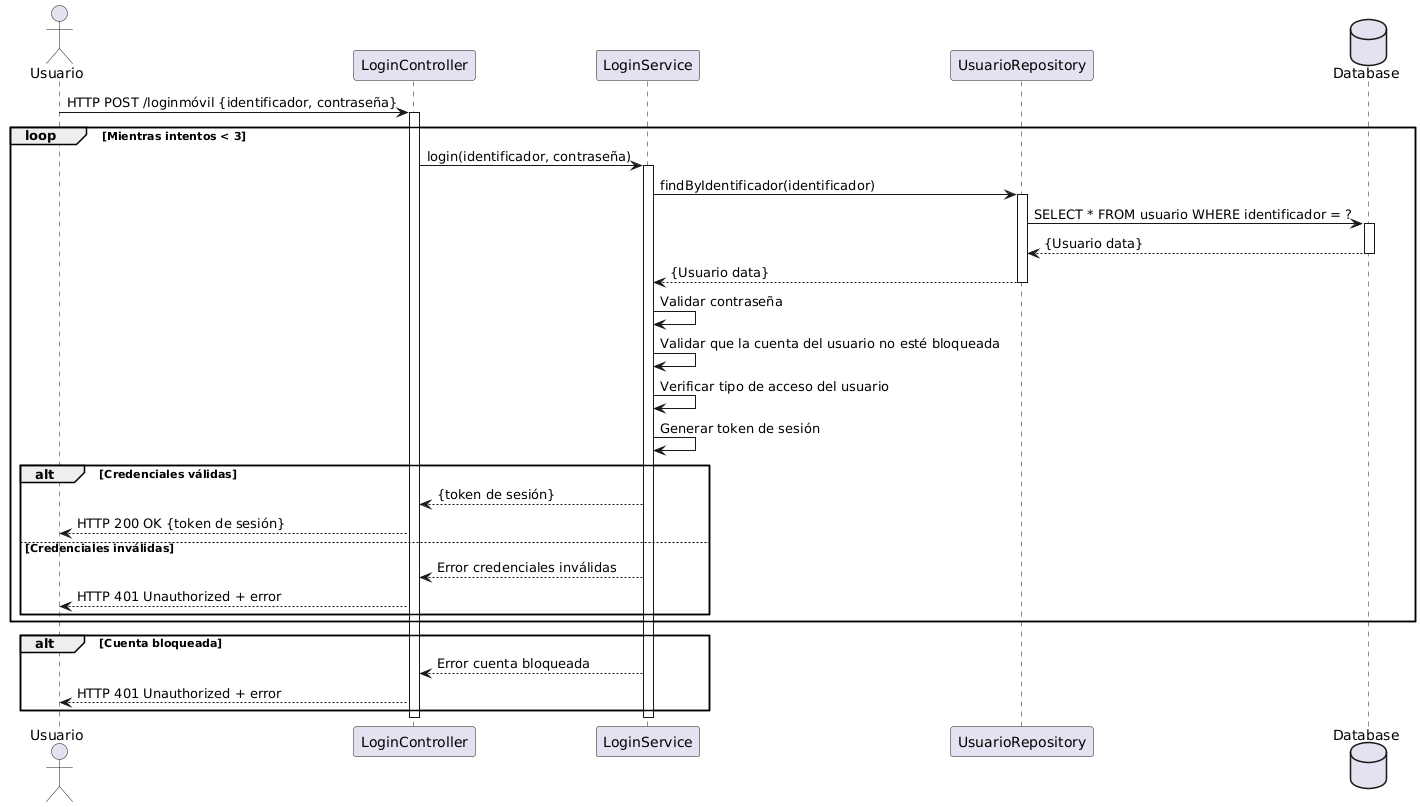
\includegraphics[width=.35\textwidth]{Secuencia/CU-41.png}}
		\caption{Diagrama de secuencia del caso de uso número 41 (CU-41).}
		\label{fig:Diagrama de secuencia CU-41}
	\end{center}
\end{figure}

\begin{figure}[htbp!]
	\begin{center}
		\fbox{\includegraphics[width=.35\textwidth]{Secuencia/CU-42.png}}
		\caption{Diagrama de secuencia del caso de uso número 42 (CU-42).}
		\label{fig:Diagrama de secuencia CU-42}
	\end{center}
\end{figure}


\chapter{Trabajo futuro}

En este capítulo se mencionará lo que se tiene planeado realizar para el siguiente periodo de TT en ella se describen las actividades que se debe realizar para el funcionamiento del sistema, además se mencionan algunas mejoras que se deben realizar

Para la implementación del backend, se utilizará Spring Boot como framework principal, permitiendo establecer una comunicación eficiente entre Kotlin y la base de datos. Se aprovecharán las diversas herramientas que ofrece Spring Boot, para facilitar la interacción con la base de datos y gestionar las operaciones. 
Ahora bien, para la implementación de la base de datos se utilizará PostgreSQL como sistema gestor de base de datos.

Por otro lado, para el desarrollo de la parte móvil se planea desarrollar una serie de puntos:
\begin{itemize}
    
    \item Implementar canales seguros DE HTTP para el intercambio de datos sensibles. 
    \item Optimizacion de métodos de lista y repositorio para mejorar el rendimiento en consultas. 
    \item Implementación de un módulo para que Kotlin envíe imágenes directamente a la BD. 
    \item Programar las pantallas del sistema. 
    \item un módulo de notificación qué permitirá a los usuarios mantener a los usuarios informados sobre las modificaciones que puedan surgir en los ETS. 
    \item Implementar un esquema de encriptacion de datos para la protección de datos.
\end{itemize}

Finalmente, con los resultados obtenidos en esta primera parte del trabajo terminal se buscará mejorar el modelo de extracción de características para la generación de embeddings que permitan realizar la identificación de usuarios siguiendo un enfoque de verificación, esto permitirá la creación de una base de datos vectorial persistente para finalmente implementar el proceso de inferencia/reconocimiento en tiempo real.

\chapter{Bibliografía}

\bibliography{ref}

\end{document}